\chapter{Projekt systemu CargoLink}
W tym rozdziale zostanie opisany projekt systemu, analiza wymagań pod kątem przypadków użycia oraz projekt bazy danych. Każdy przypadek użycia zostanie omówiony, a jego działanie zilustrowane za pomocą makiet aplikacji. Przygotowana została makieta aplikacji w wersji na telefony komórkowe oraz wersja na standardowe monitory. Pierwszym podpunktem w nowym rozdziale będzie identyfikacja aktorów. Jest to kluczowy element w projektowaniu diagramu przypadków użycia aplikacji.

\section{Identyfikacja aktorów}
Biorąc pod uwagę wymagania opisane w poprzednich podrozdziałach, zaprojektowany został diagram przypadków użycia aplikacji. W systemie wyróżnić można następujących aktorów:
\begin{enumerate}
\item \textbf{Użytkownik niezalogowany} - nowy gość w serwisie, może  się zalogować oraz przeglądać ogłoszenia przewozu i zlecenia dodane przez pozostałych użytkowników.
\item \textbf{Przewoźnik} - aktor odpowiedzialny za transport towarów. Przewoźnik może przeglądać dostępne zlecenia, dodawać ogłoszenia o planowanych trasach, komunikować się z autorami ogłoszeń, przyjmować zlecenia oraz oceniać i komentować kontrahentów.
\item \textbf{Zleceniodawca} - użytkownik systemu, który zleca transport towarów. zleceniodawca może dodawać nowe zlecenia transportowe, podobnie jak przewoźnik, może również przeglądać ogłoszenia przewoźników oraz komunikować się z autorami ogłoszeń.
\item \textbf{Moderator} - osoba odpowiedzialna za zarządzanie systemem. Moderator zatwierdza lub usuwa nowe ogłoszenia i zlecenia.
\item \textbf{Administrator} - użytkownik umiejscowiony najwyżej w hierarchii systemu. Może on wykonywać wszystko co moderator oraz ma możliwość dodawania nowych moderatorów lub usuwania obecnych.
\end{enumerate}

\section{Projekt interfejsu użytkownika}
Makieta aplikacji została wykonana w darmowym programie \texttt{Figma}, który pozwala na tworzenie interfejsu użytkownika i oferuje wiele funkcji ułatwiających pracę, takich jak utrzymanie spójności w rozmiarach czcionek, kolorach czy odstępach. Figma świetnie nadaje się także do tworzenia komponentów wielokrotnego użytku oraz ich wariantów. Komponenty te są również wykorzystywane w frameworku \texttt{Next.js}, dlatego uwzględnienie ich już na etapie projektowania ułatwia późniejszą implementację w kodzie.

Poniżej znajdują się założenia wizualne, które zostaną zastosowane podczas projektowania makiety aplikacji. Zdefiniowane zostały wartości takie jak:
\begin{itemize}
    \item rozmiary czcionek dla odpowiednich elementów aplikacji,
    \item paleta kolorów,
    \item trzy warianty przycisków, główny, drugorzędny oraz trzeciorzędny,
    \item wygląd hiperłącz na stronie,
    \item przycisk do wybierania wersji językowej,
    \item warianty odstępów między elementami,
    \item pola tekstowe (ang. \texttt{inputs}) wraz ze swoim drugim wariantem,
    \item pola jednokrotnego wyboru.
\end{itemize}
\begin{figure}[H]
	\centering
		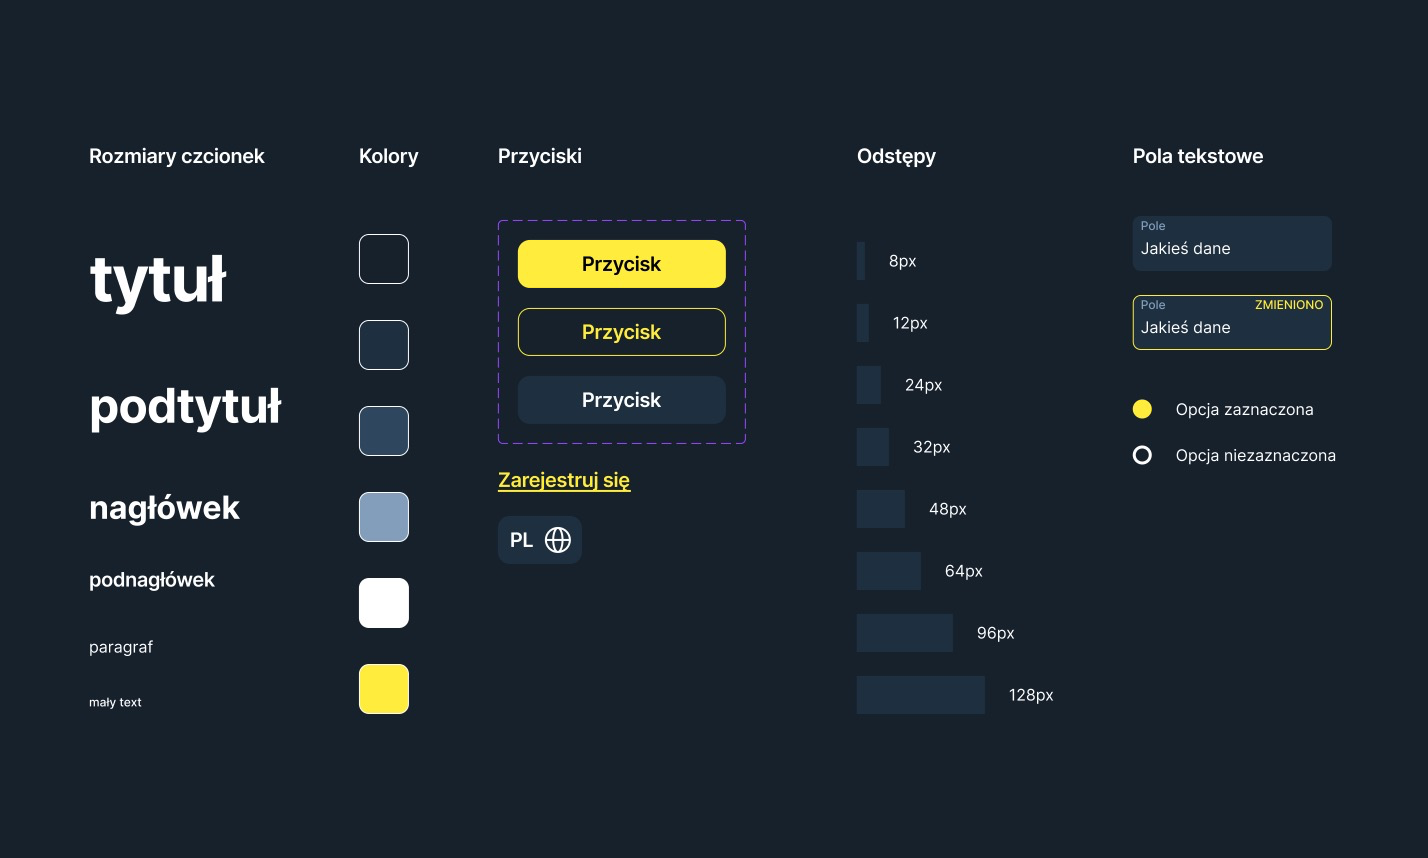
\includegraphics[width=1\linewidth]{rozdzial1/komponenty.png}
	\caption{Wybrane parametry dotyczące interfejsu użytkownika}
	\label{Rys. fig:Wybrane parametry dotyczące interfejsu użytkownika}
\end{figure}
Parametry te pozwolą na ujednolicenie wyglądu interfejsu, co przełoży się na lepsze odczucia podczas korzystania z aplikacji.

\section{Diagramy przypadków użycia}
W tym podrozdziale przedstawione zostaną diagramy przypadków użycia serwisu \texttt{CargoLink}, korzystając z definicji aktorów opisanych powyżej. Dodatkowo opisane i graficznie przedstawione zostaną wszystkie przypadki użycia użyte w diagramach.
\subsection{Niezalogowany użytkownik}
\begin{figure}[H]
	\centering
		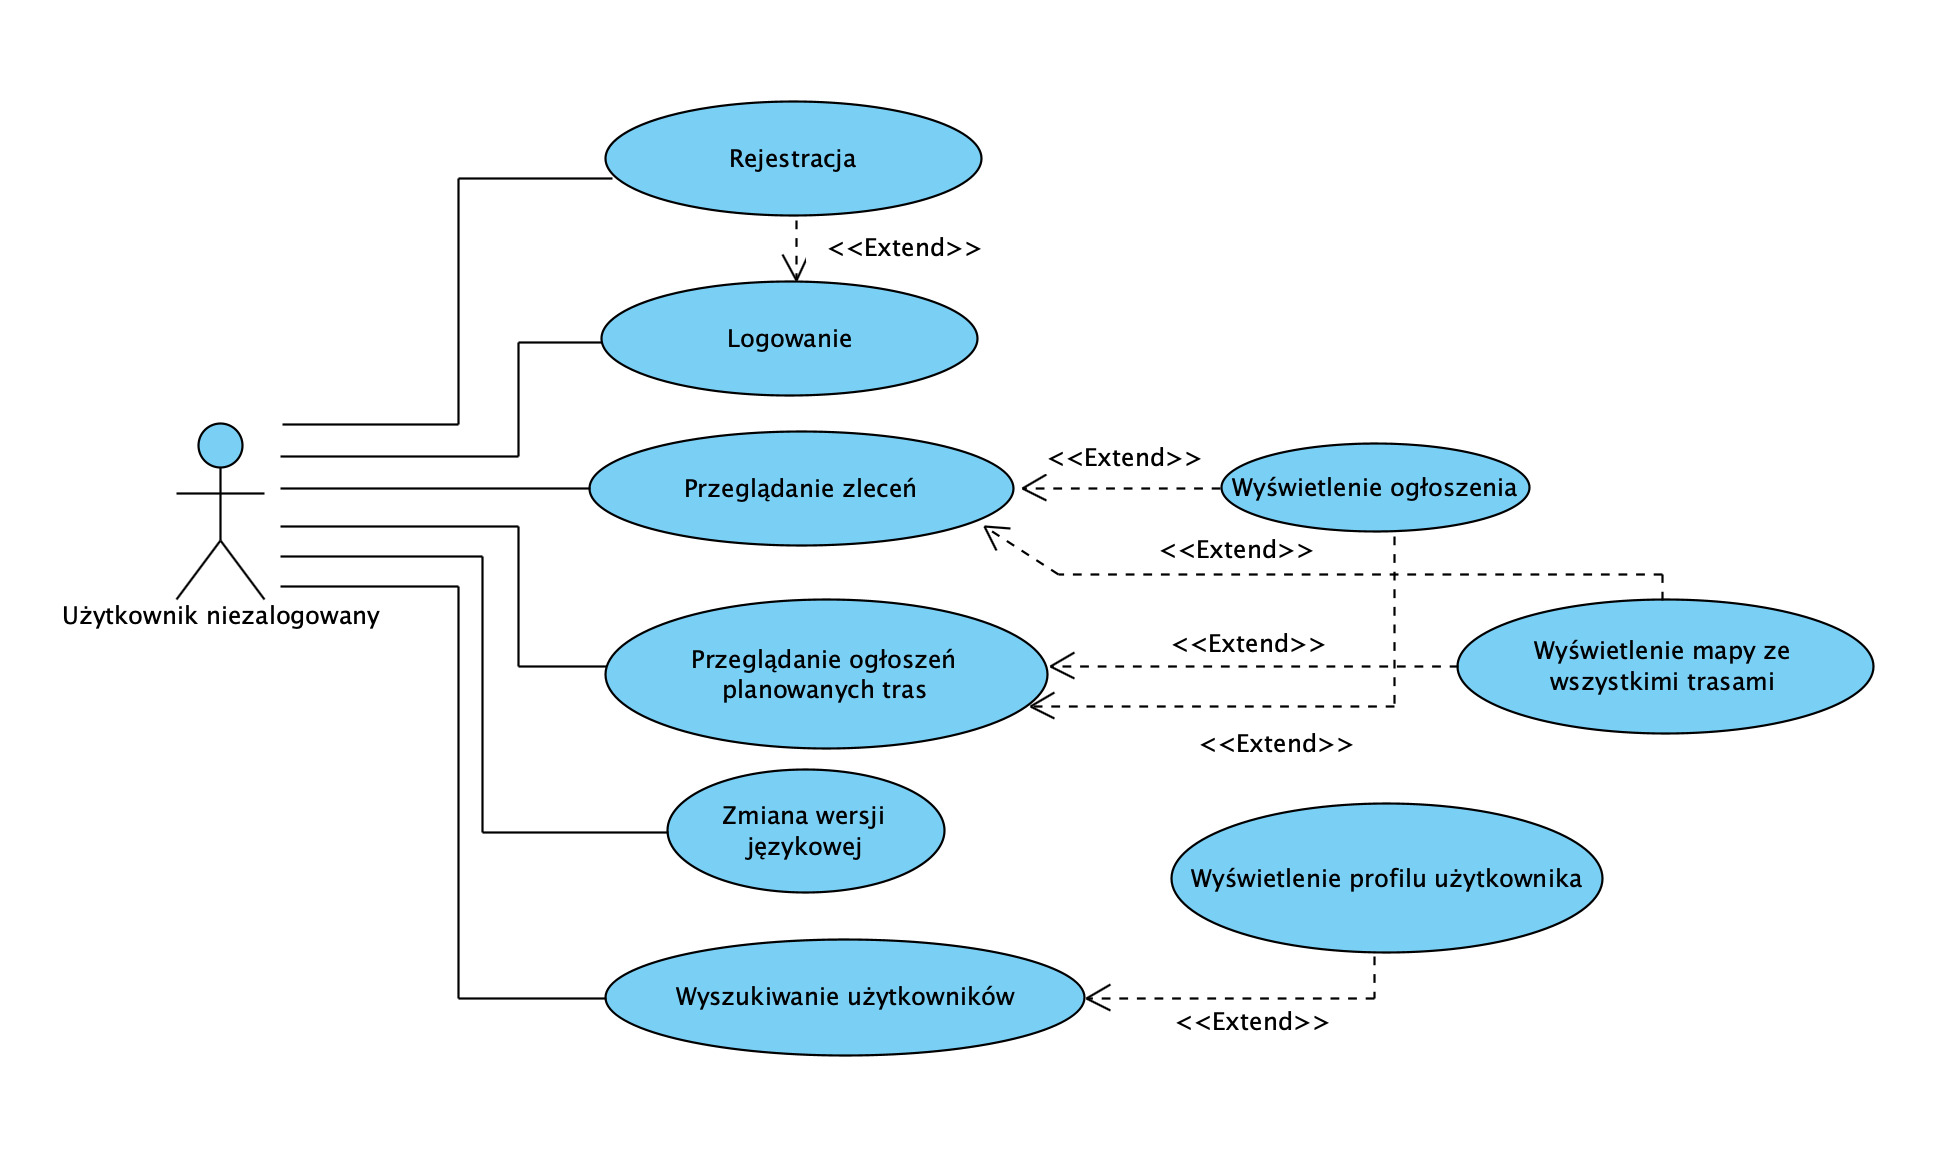
\includegraphics[width=\linewidth]{rozdzial1/PU_niezalogowany_uzytkownik.jpg}
	\caption{Diagram przedstawiający przypadki użycia aktora \texttt{Niezalogowany użytkownik}}
	\label{Rys. fig:Diagram przedstawiający przypadki użycia aktora Niezalogowany użytkownik}
\end{figure}
Na powyższym diagramie przedstawione zostały przypadki użycia dla \texttt{Niezalogowanego użytkownika}. \\

\texttt{Rejestracja} \\
Zdarzenie inicjujące: Kliknięcie przycisku \texttt{Nie masz konta? Zarejestruj się}. \\
Warunki początkowe: Użytkownik nie jest zalogowany. \\
Przebieg podstawowy realizacji przypadku użycia:
\begin{enumerate}
    \item Kliknięcie przycisku \texttt{Nie masz konta? Zarejestruj się} (Rys. \ref{fig:Formularz rejestracji - abc - mobile}.a lub \ref{fig:Formularz rejestracji - ab - desktop}.a);
    \item Wybór typu konta: zleceniodawca lub przewoźnik;
    \item Kliknięcie przycisku \texttt{dalej} (Rys. \ref{fig:Formularz rejestracji - abc - mobile}.b lub \ref{fig:Formularz rejestracji - ab - desktop}.b);
    \item Wpisanie danych:
        \begin{itemize}
            \item imię,
            \item nazwisko,
            \item email (dwukrotnie w celu potwierdzenia),
            \item adres, miasto i ulica (w celu generowania umów między użytkownikami),
            \item numer telefonu,
            \item hasło (dwukrotnie w celu potwierdzenia)
        \end{itemize}
    \item Kliknięcie przycisku \texttt{Dalej}; (Rys. \ref{fig:Formularz rejestracji - abc - mobile}.c lub \ref{fig:Formularz rejestracji - c - desktop})
    \item System sprawdza w bazie danych czy istnieje już użytkownik o podanym emailu oraz sprawdza poprawność wprowadzonych danych;
    \item Wybór czy konto ma reprezentować przedsiębiorstwo (wymagane będzie podane pełnej nazwy firmy, wraz z NIP'em oraz adresem siedziby), bądź osobę fizyczną;
    \item Jeżeli wybrane zostało przedsiębiorstwo, system sprawdza poprawność wprowadzonych danych;
    \item Kliknięcie przycisku \texttt{Dalej}; (Rys. \ref{fig:Formularz rejestracji - ab2 - mobile}.a lub \ref{fig:Formularz rejestracji - ab2 - desktop}.a)
    \item Zaznaczenie języków, którymi użytkownik umie się posługiwać (informacje te pokazywać się będą w oknie czatu oraz na profilu, aby ułatwić użytkownikom porozumienie się);
    \item Akcpetacja regulaminu;
    \item Kliknięcie przycisku \texttt{Zarejestruj się}; (Rys. \ref{fig:Formularz rejestracji - ab2 - mobile}.a lub \ref{fig:Formularz rejestracji - ab2 - desktop}.a)
\end{enumerate}
Przebieg alternatywny realizacji podpunktu (6a): W bazie danych istnieje już użytkownik o podanym emailu bądź użytkownik podał błędne dane. System informuje o niezgodności. \\
Przebieg alternatywny realizacja podpunktu (7a): Jeżeli konto ma reprezentować osobę fizyczną, pola do wpisania informacji o przedsiębiorstwie nie wyświetlą się. \\
Warunki końcowe: Dodanie utworzonego użytkownika do bazy, a następnie przekierowanie go na przeglądarkę ogłoszeń o planowanych trasach lub zleceń, w zależności od typu konta.
\begin{figure}[H]
 \centering
  \begin{tabular}{@{}ccc@{}}
  a) & b) & c)\\
  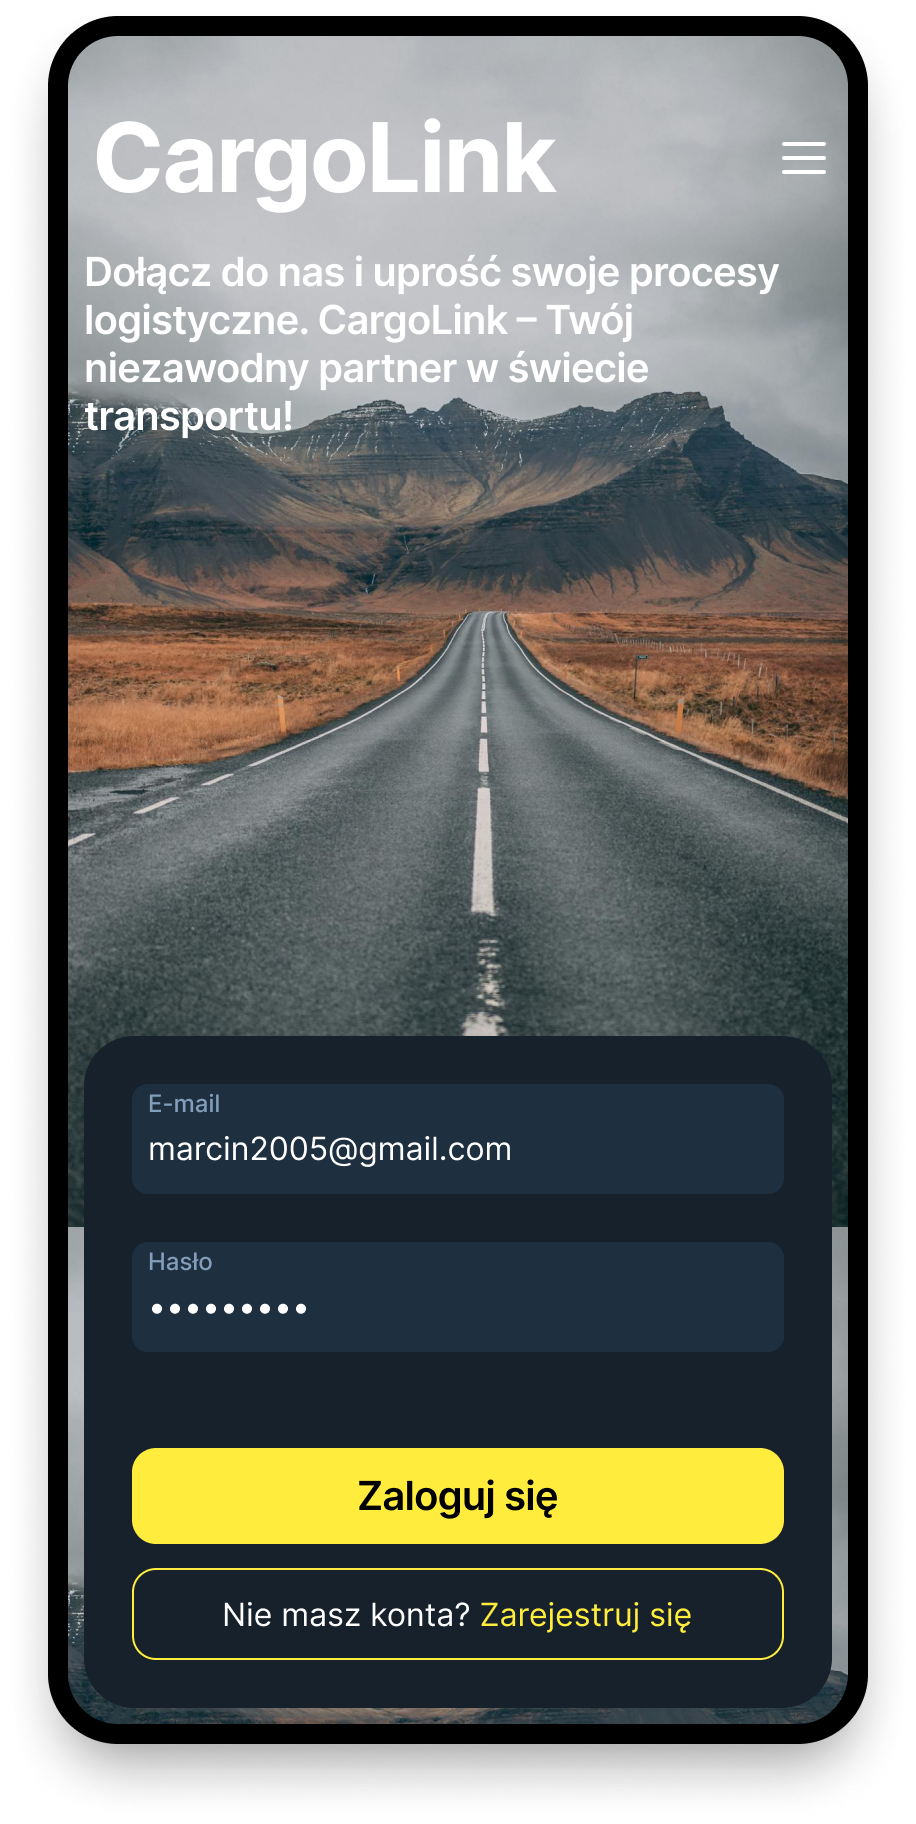
\includegraphics[width=0.3\textwidth]{rozdzial1/logowanie_m.png} &
  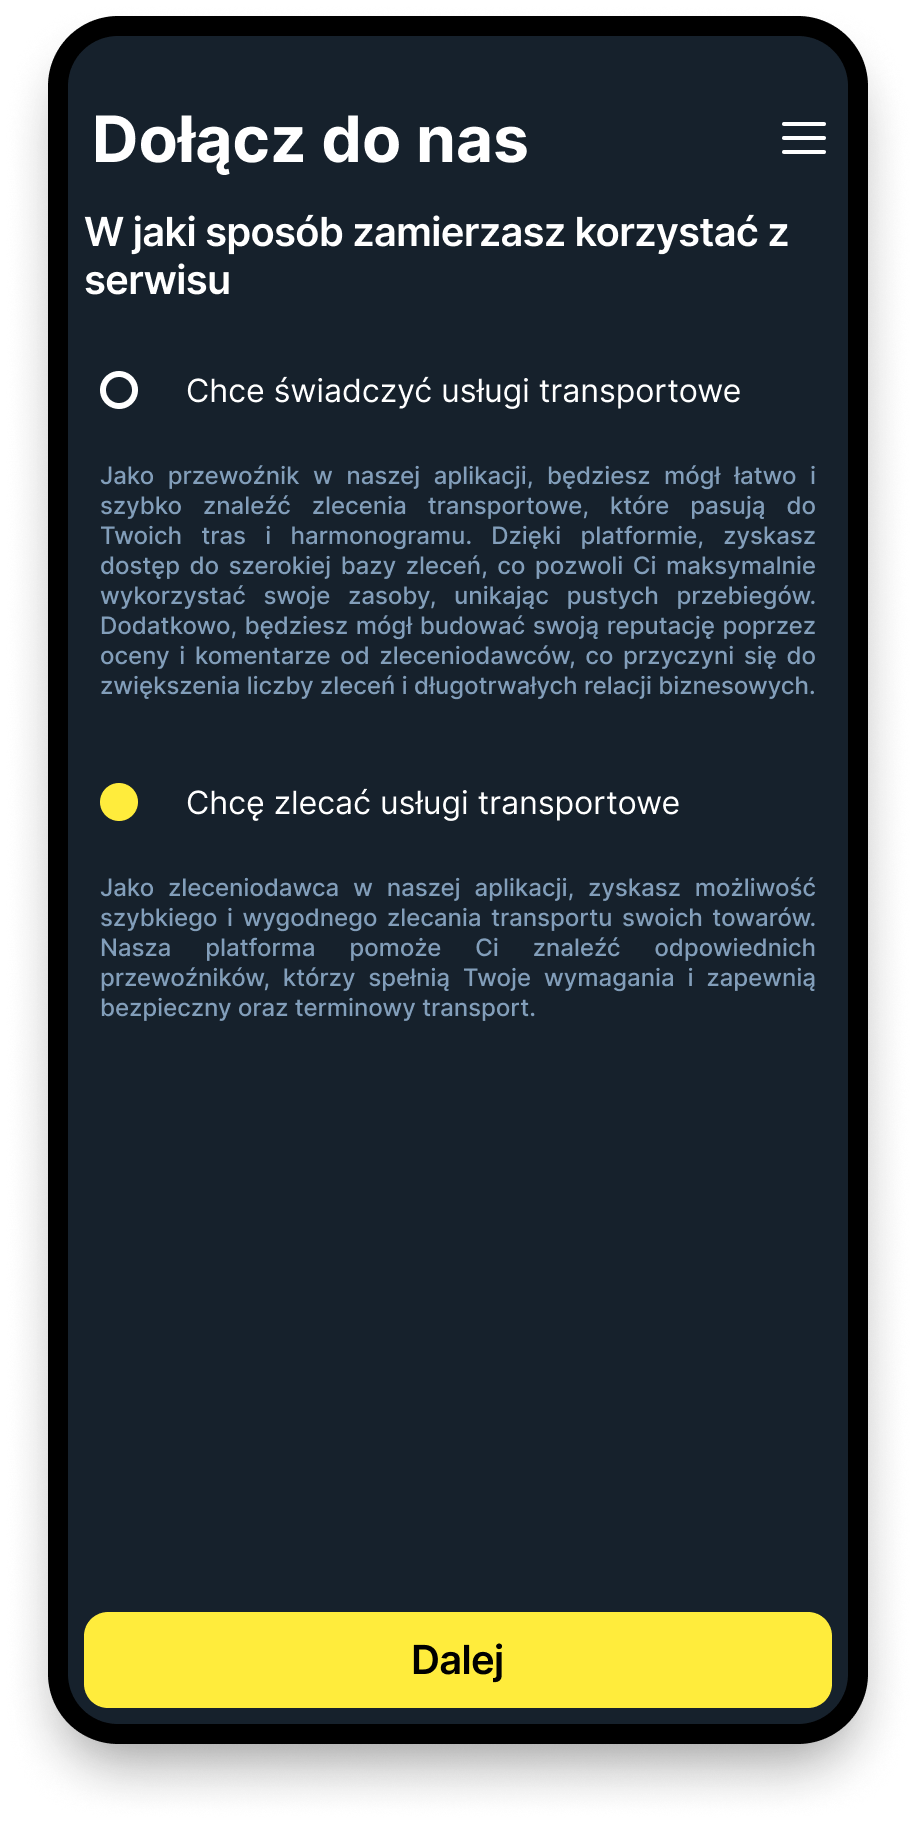
\includegraphics[width=0.3\textwidth]{rozdzial1/wybor_1_m.png} &
  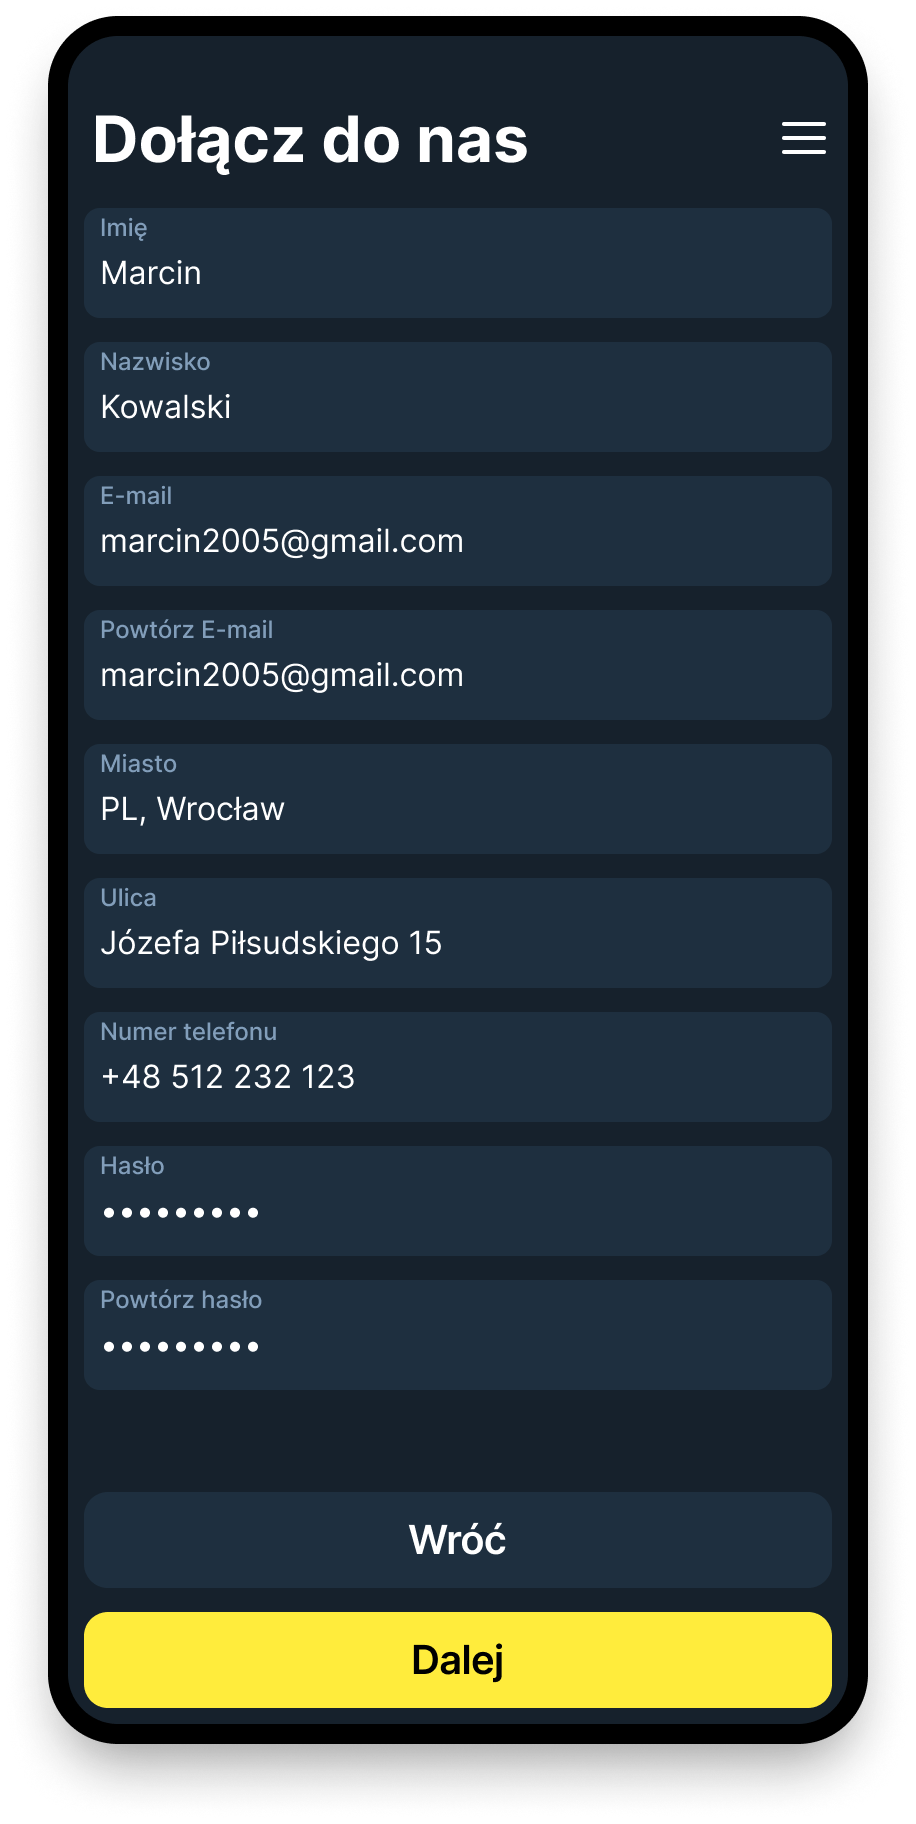
\includegraphics[width=0.3\textwidth]{rozdzial1/rejestracja_m.png}
  \end{tabular}
 \caption{Formularz rejestracji w wersji mobilnej: a) Menu logowania, b) Wybór typu konta, c) Wprowadzenie danych do rejestracji}
 \label{fig:Formularz rejestracji - abc - mobile}
\end{figure}
\begin{figure}[H]
 \centering
  \begin{tabular}{@{}ccc@{}}
  a) & b)\\
  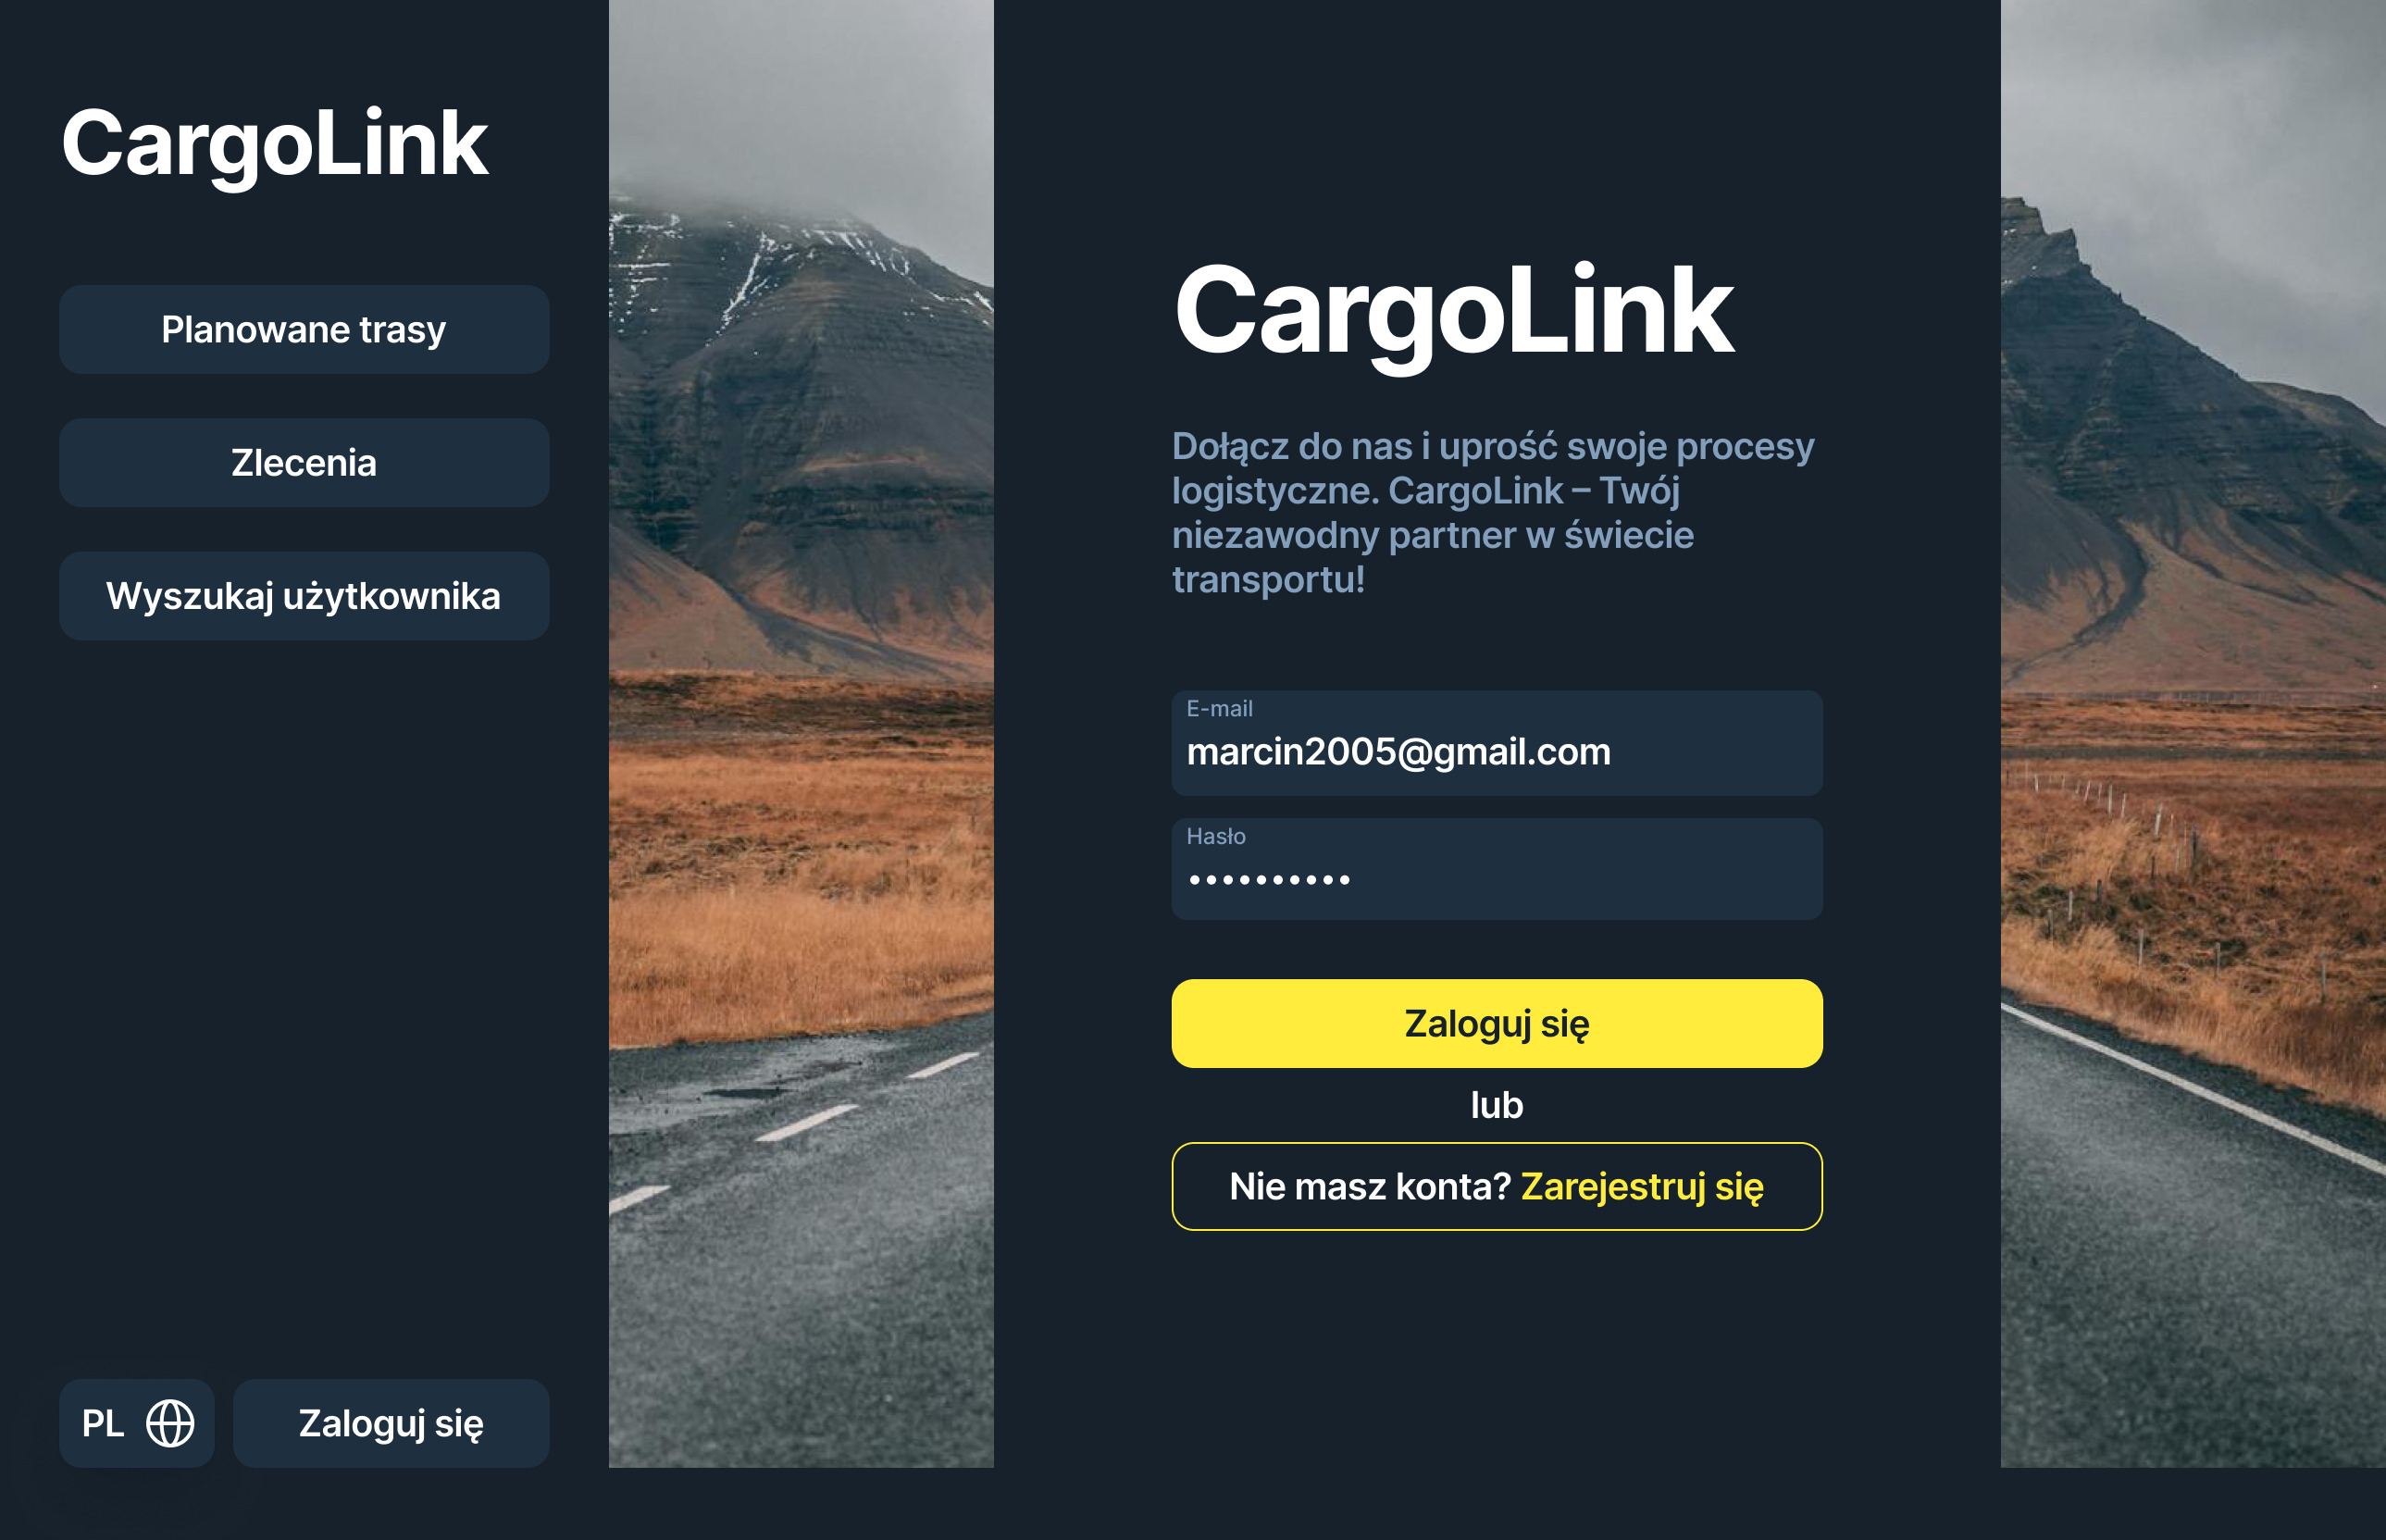
\includegraphics[width=0.45\textwidth]{rozdzial1/logowanie_d.jpg} &
  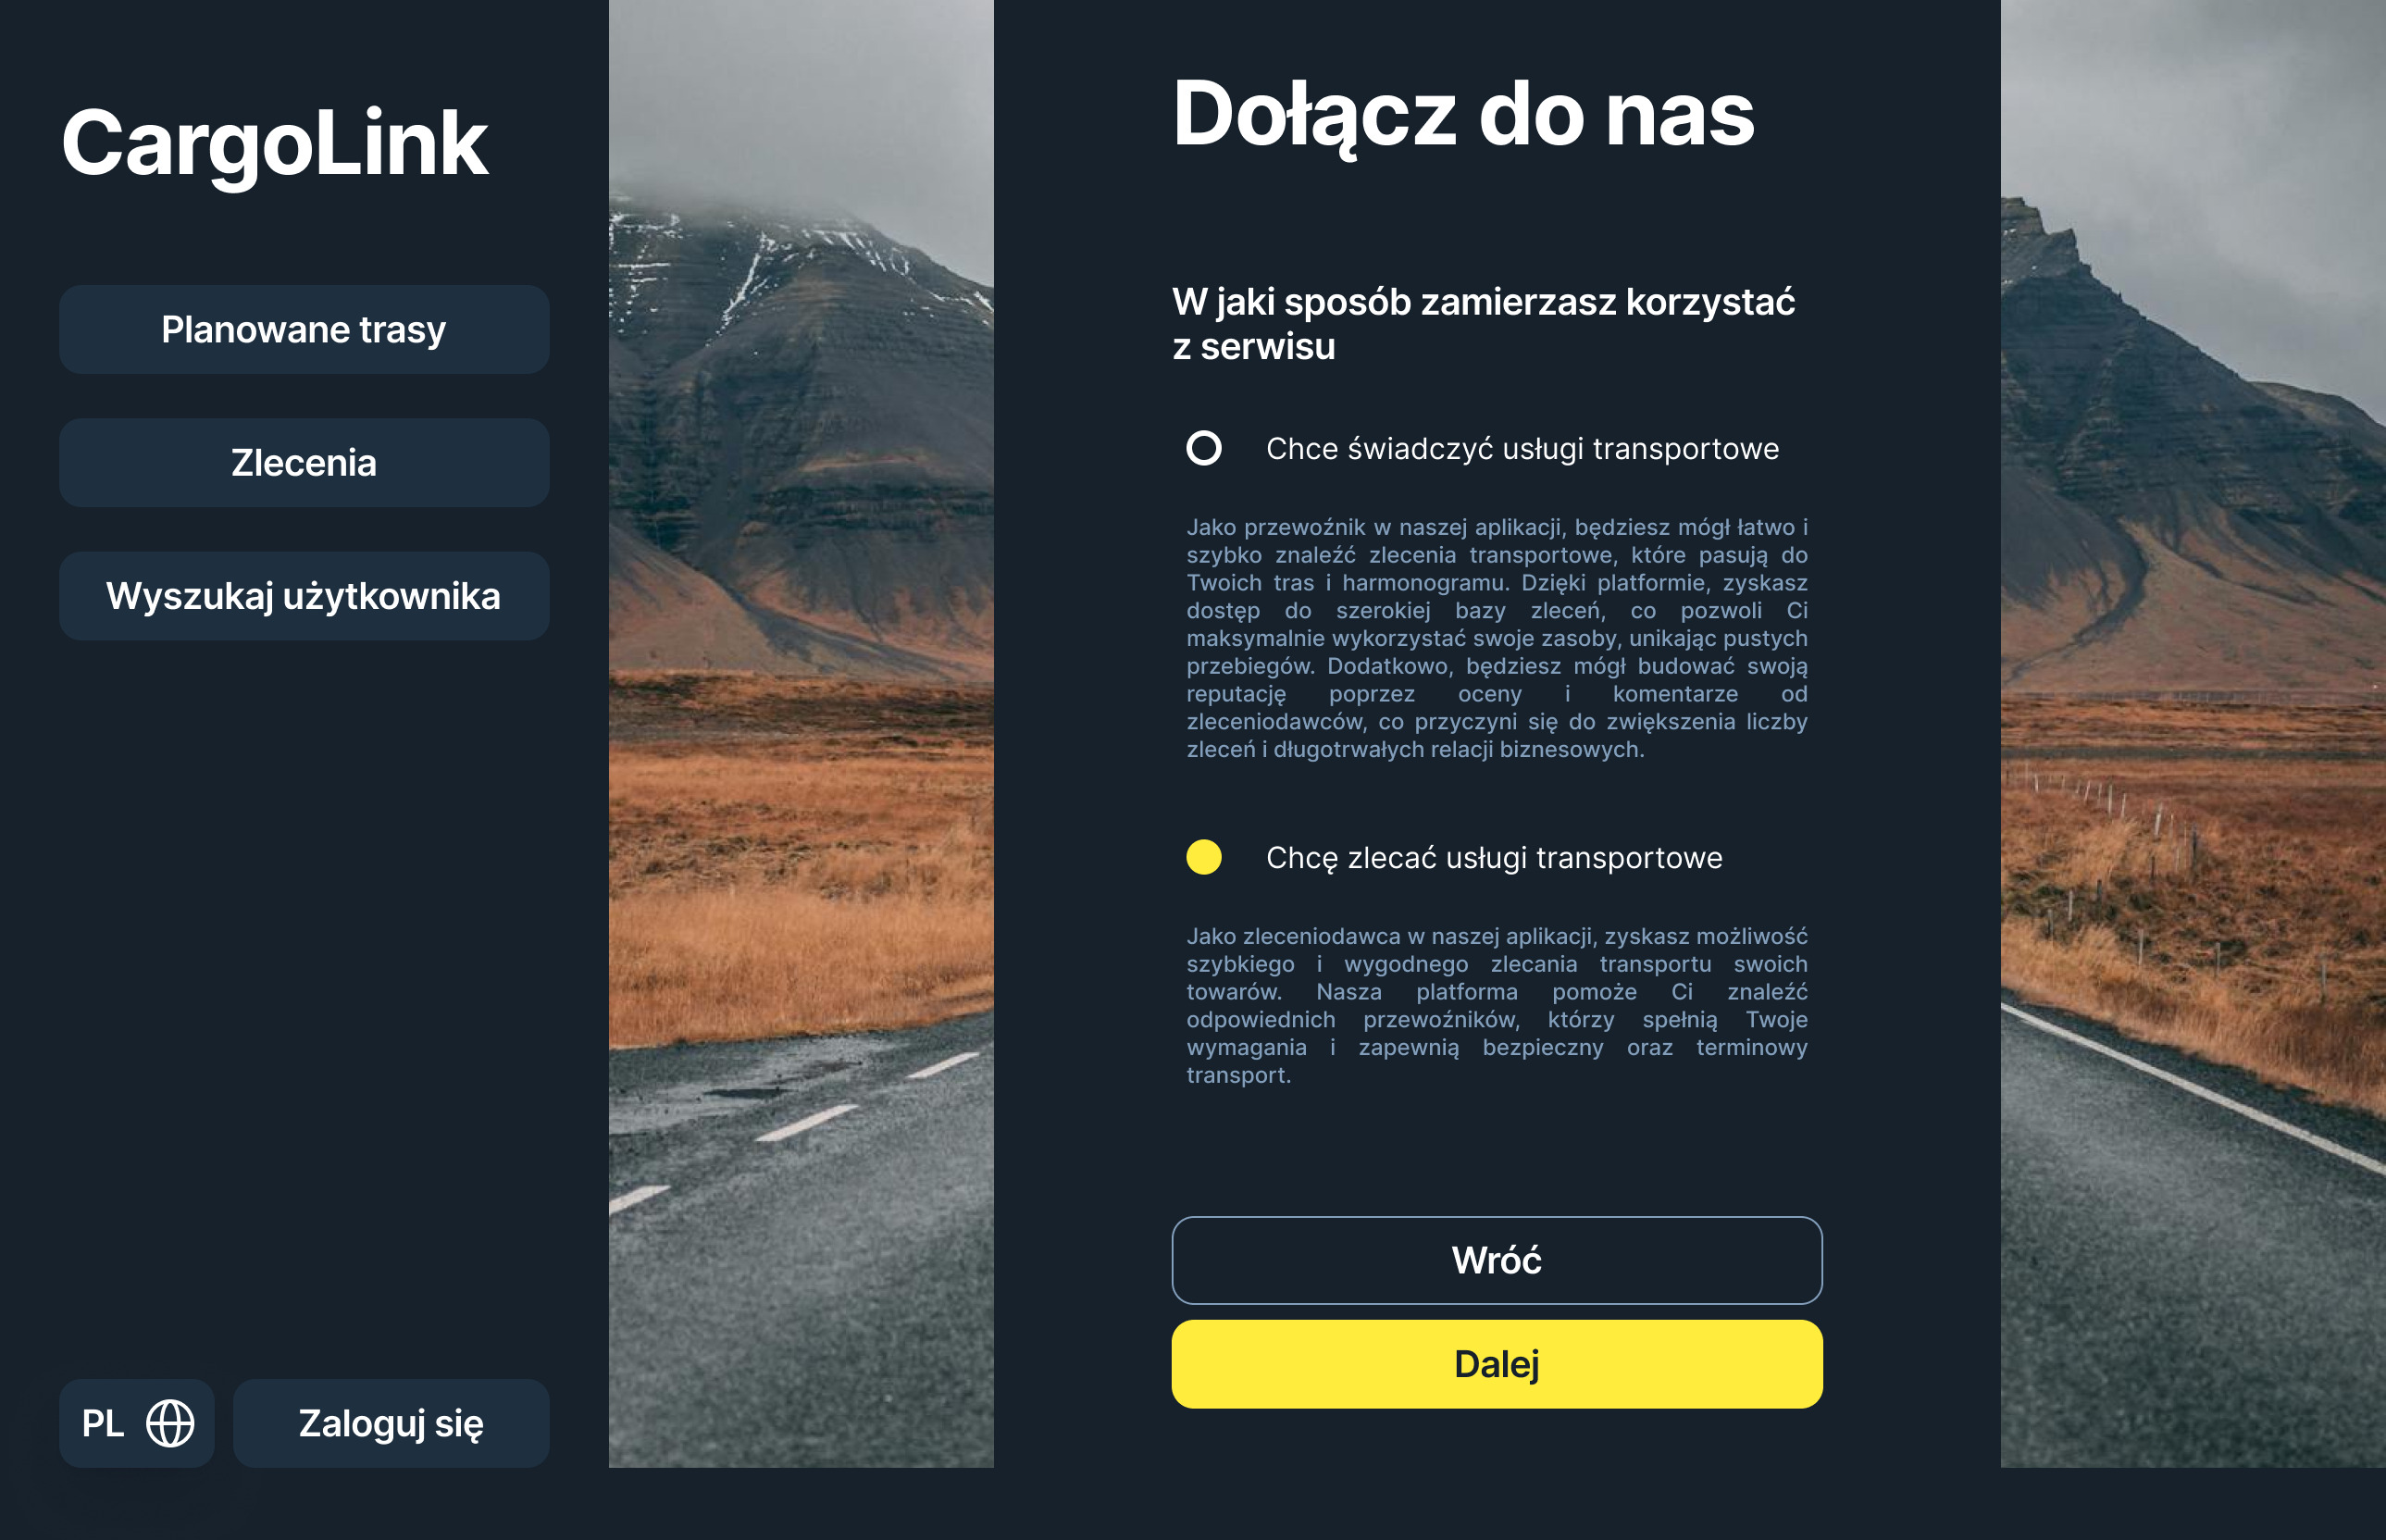
\includegraphics[width=0.45\textwidth]{rozdzial1/wybor_1_d.jpg}
  \end{tabular}
 \caption{Formularz rejestracji w wersji desktopowej: a) Menu logowania, b) Wybór typu konta}
 \label{fig:Formularz rejestracji - ab - desktop}
\end{figure}
\begin{figure}[H]
 \centering
  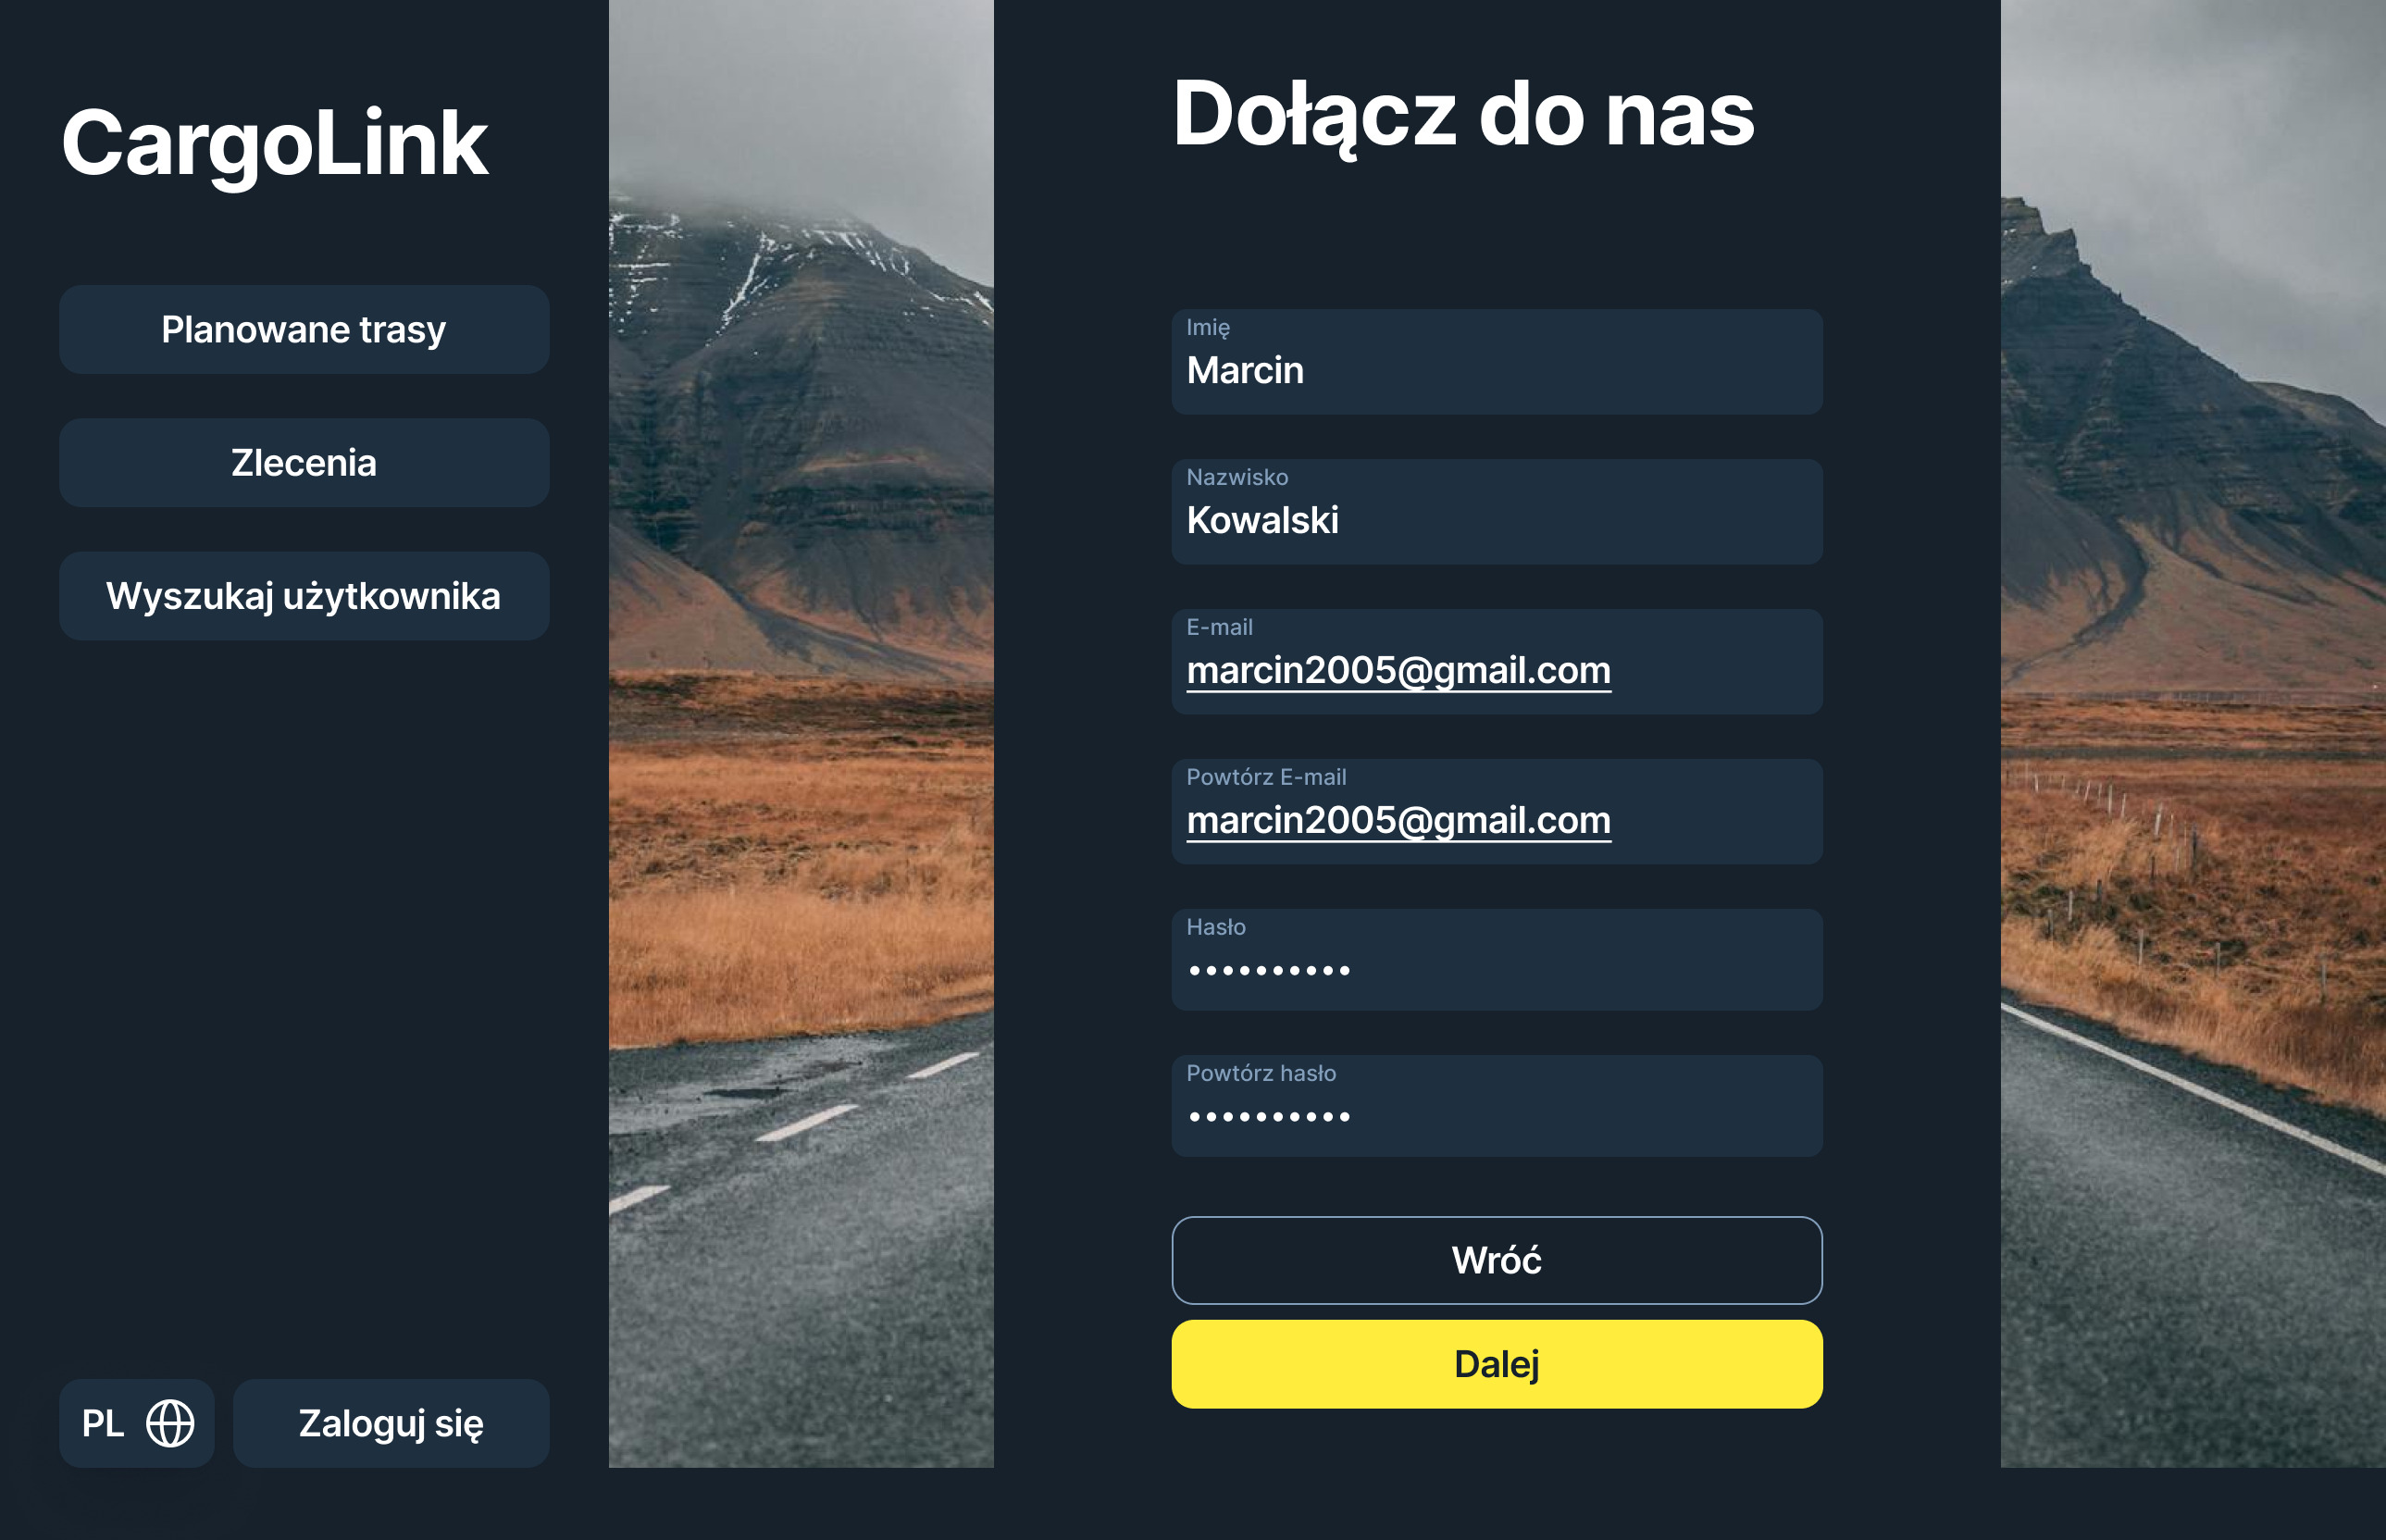
\includegraphics[width=0.7\textwidth]{rozdzial1/rejestracja_d.jpg}
 \caption{Formularz rejestracji w wersji desktopowej: Wprowadzenie danych do rejestracji}
 \label{fig:Formularz rejestracji - c - desktop}
\end{figure}
\begin{figure}[H]
 \centering
  \begin{tabular}{@{}ccc@{}}
  a) & b)\\
  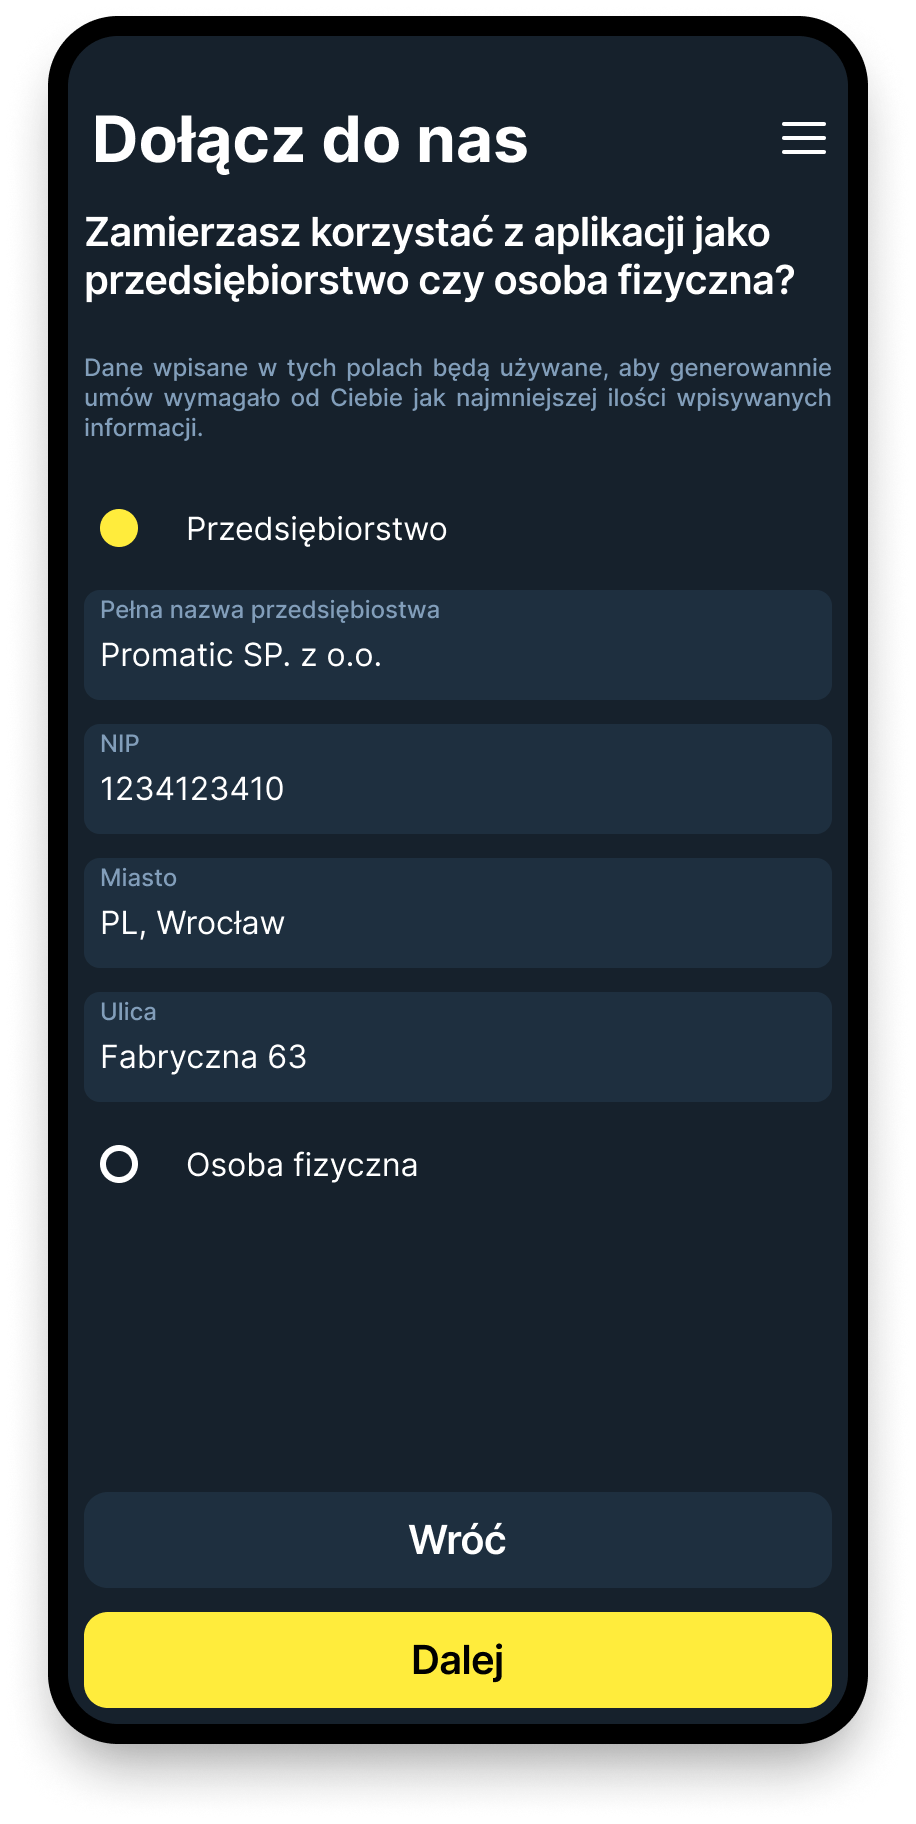
\includegraphics[width=0.3\textwidth]{rozdzial1/wybor_2_m.png} &
  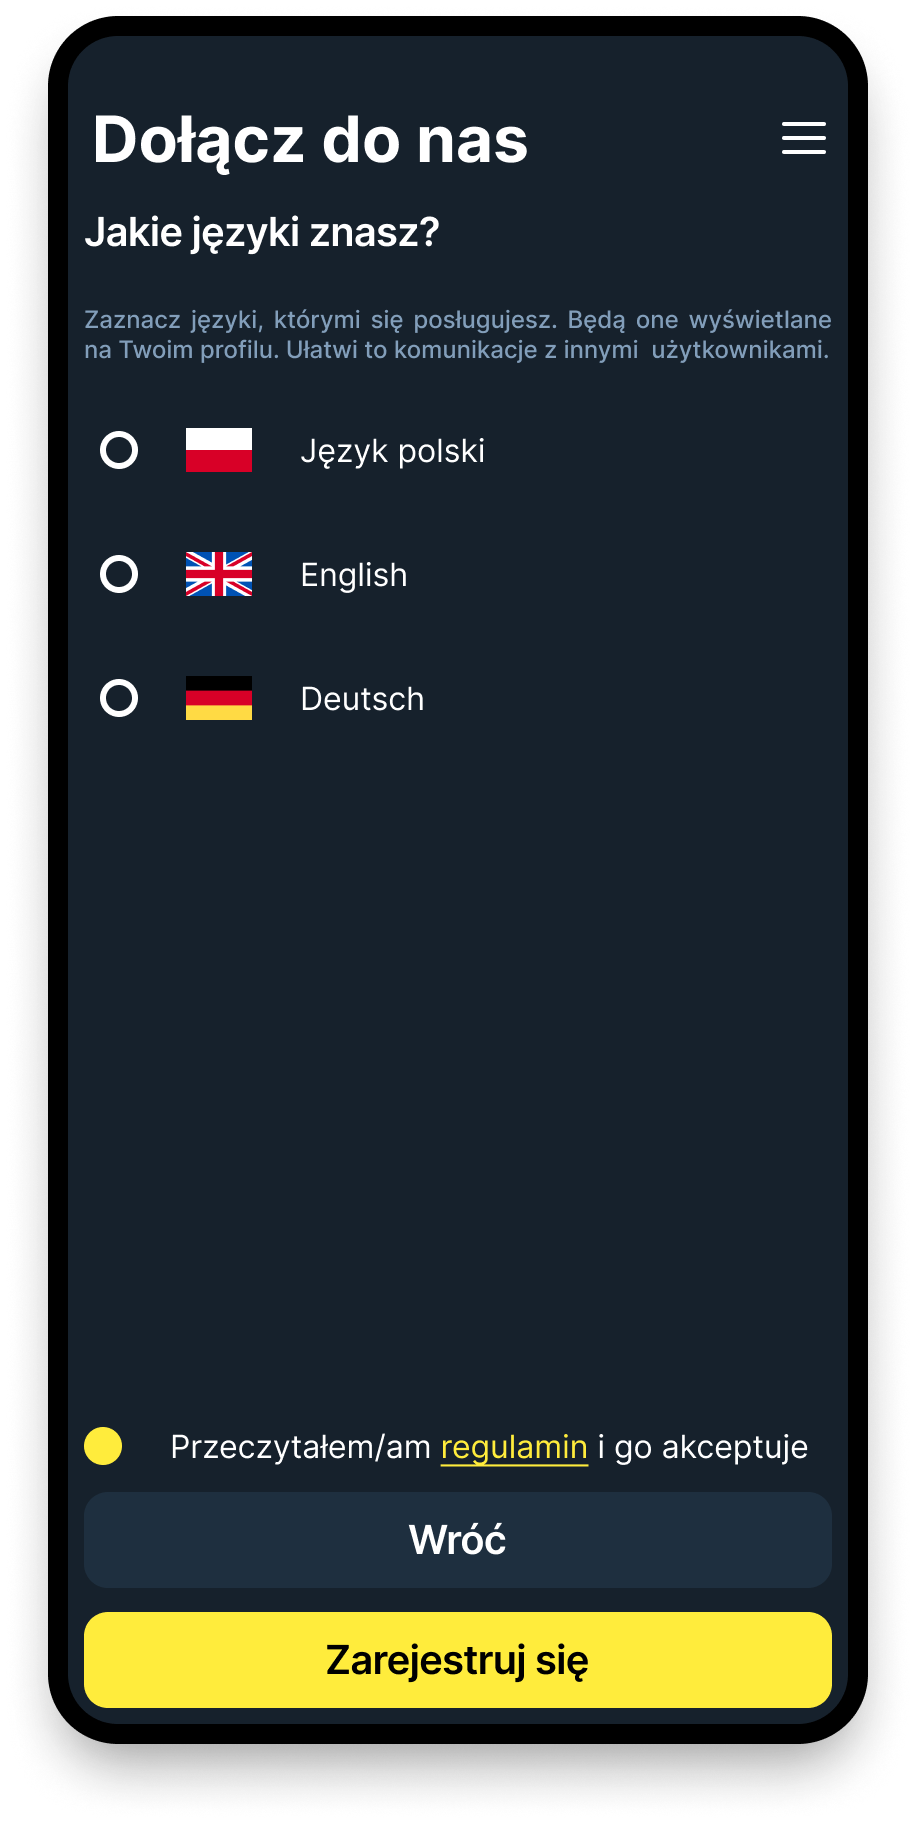
\includegraphics[width=0.3\textwidth]{rozdzial1/wybor_3_m.png}
  \end{tabular}
 \caption{Formularz rejestracji w wersji mobilnej: a) Wybór reprezentacji konta, b) Wybór języków, którymi użytkownik się posługuje, }
 \label{fig:Formularz rejestracji - ab2 - mobile}
\end{figure}
\begin{figure}[H]
 \centering
  \begin{tabular}{@{}ccc@{}}
  a) & b)\\
  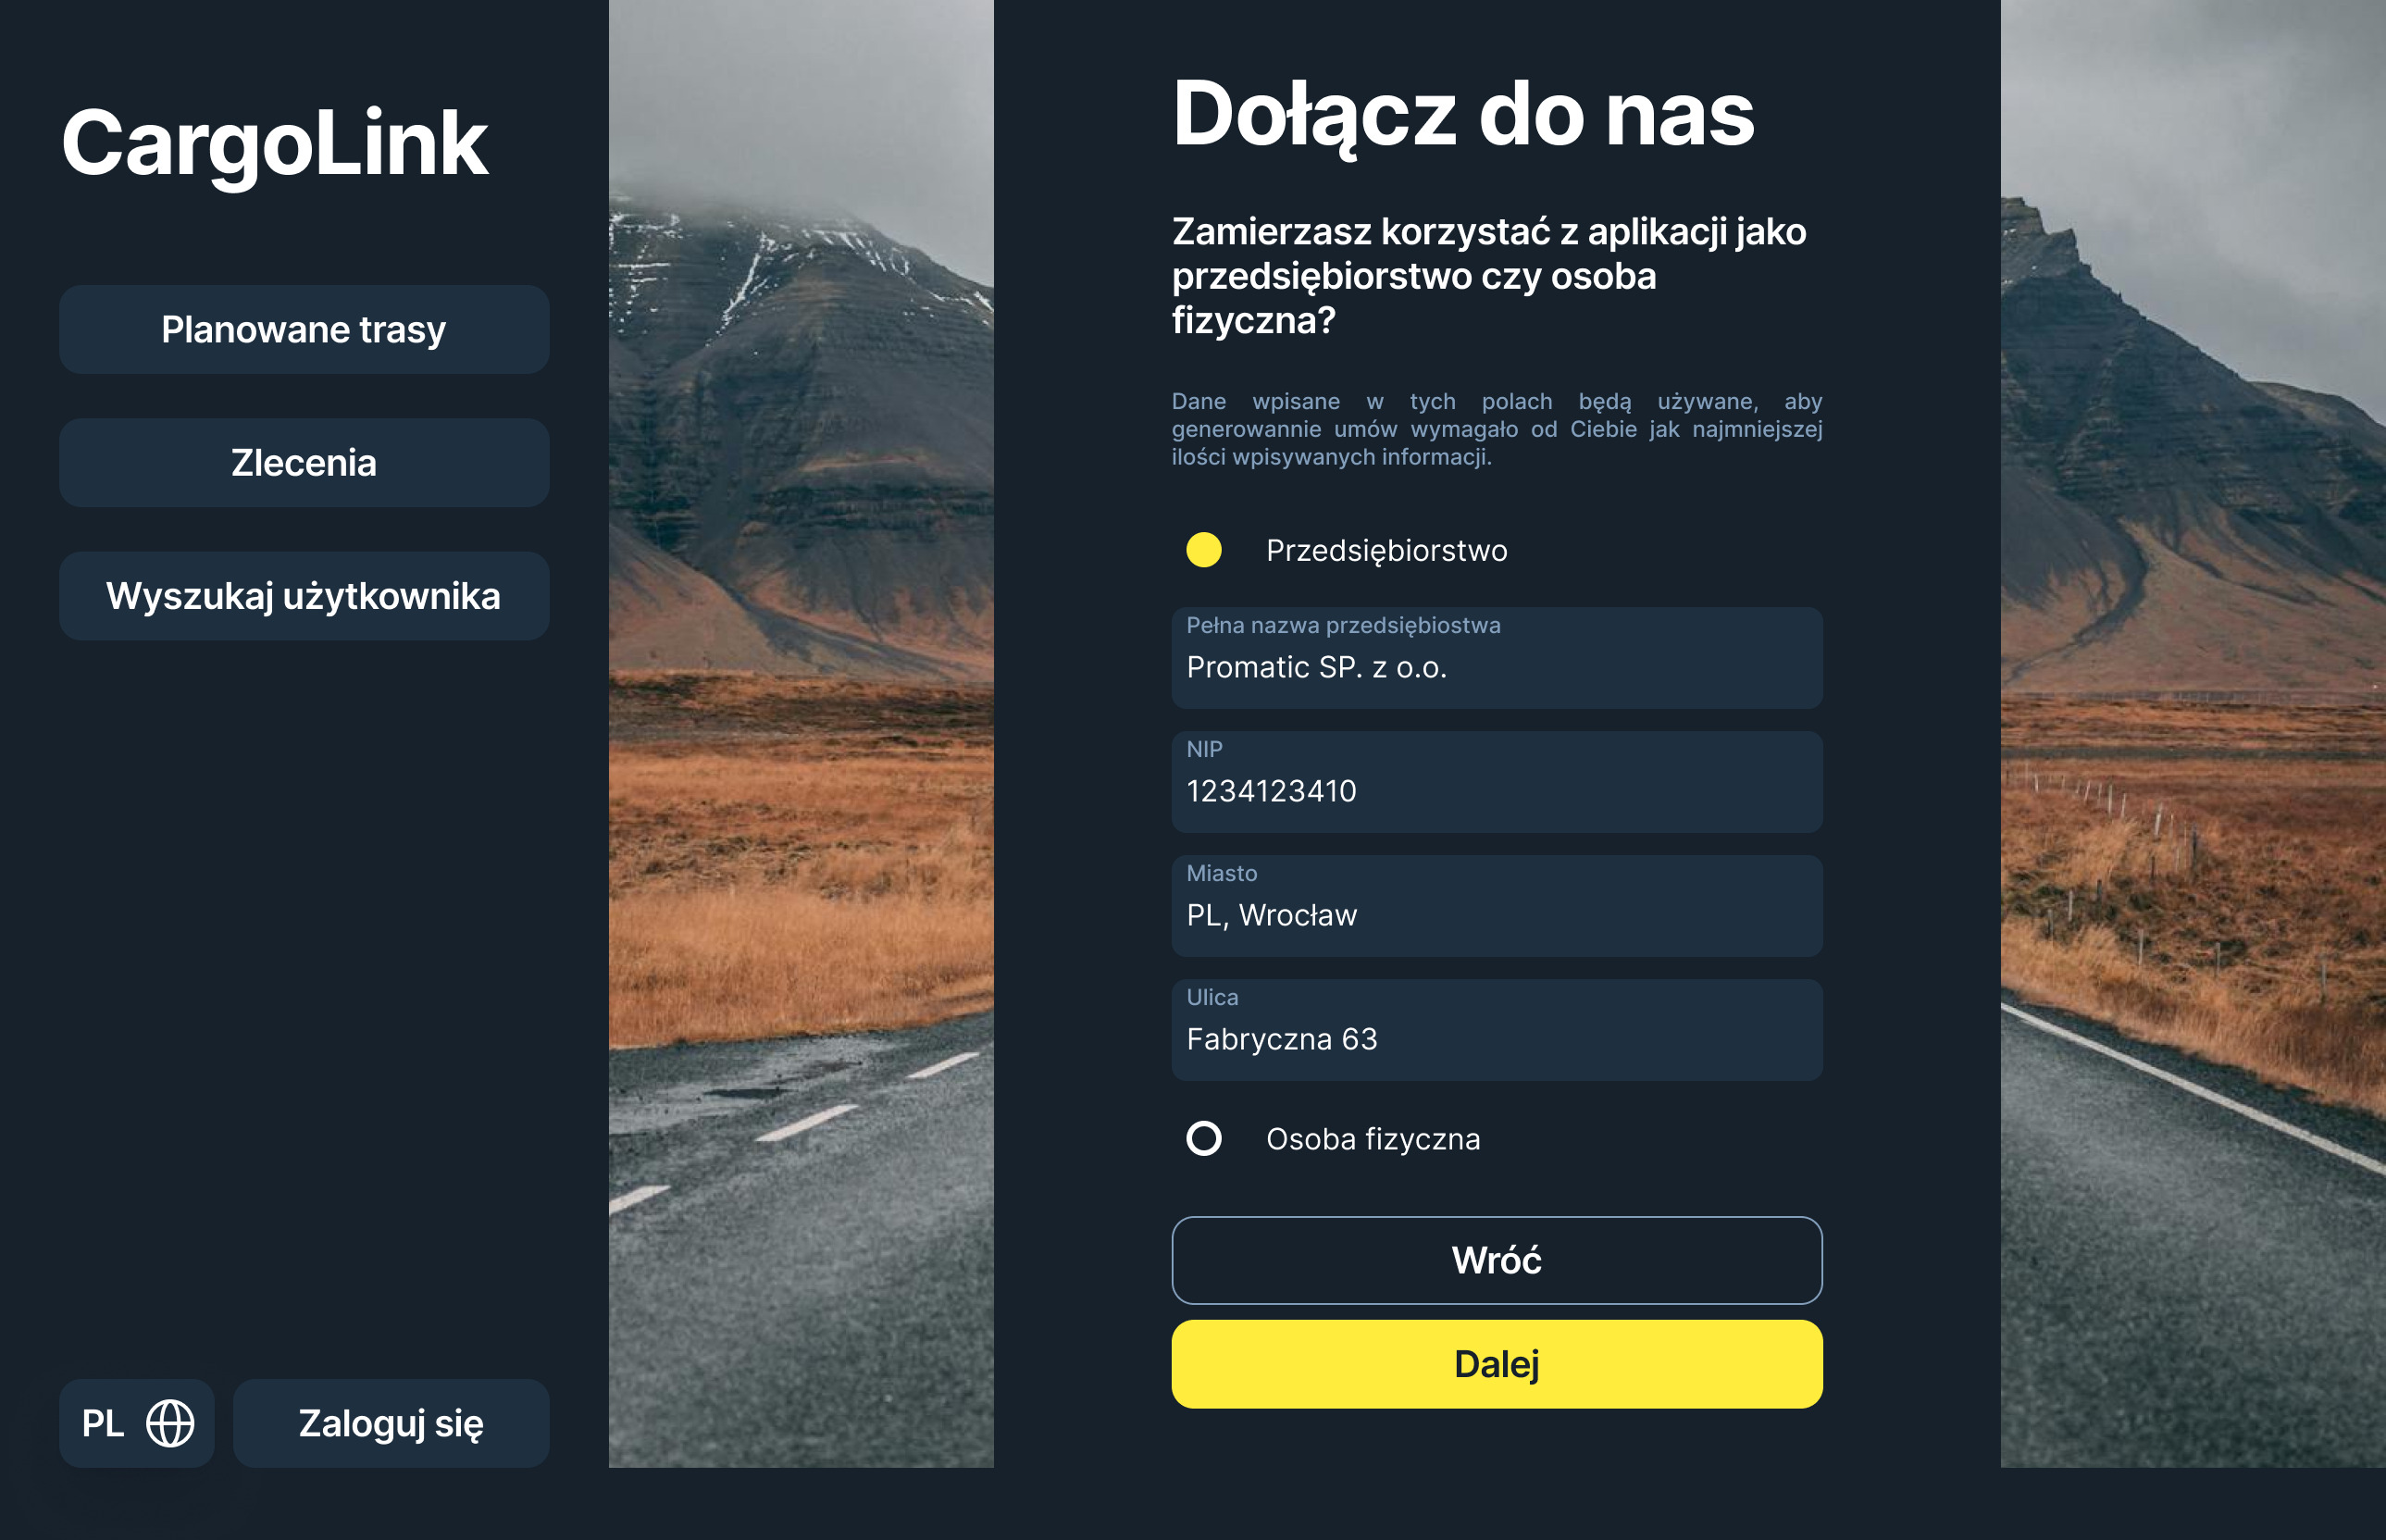
\includegraphics[width=0.45\textwidth]{rozdzial1/wybor_2_d.jpg} &
  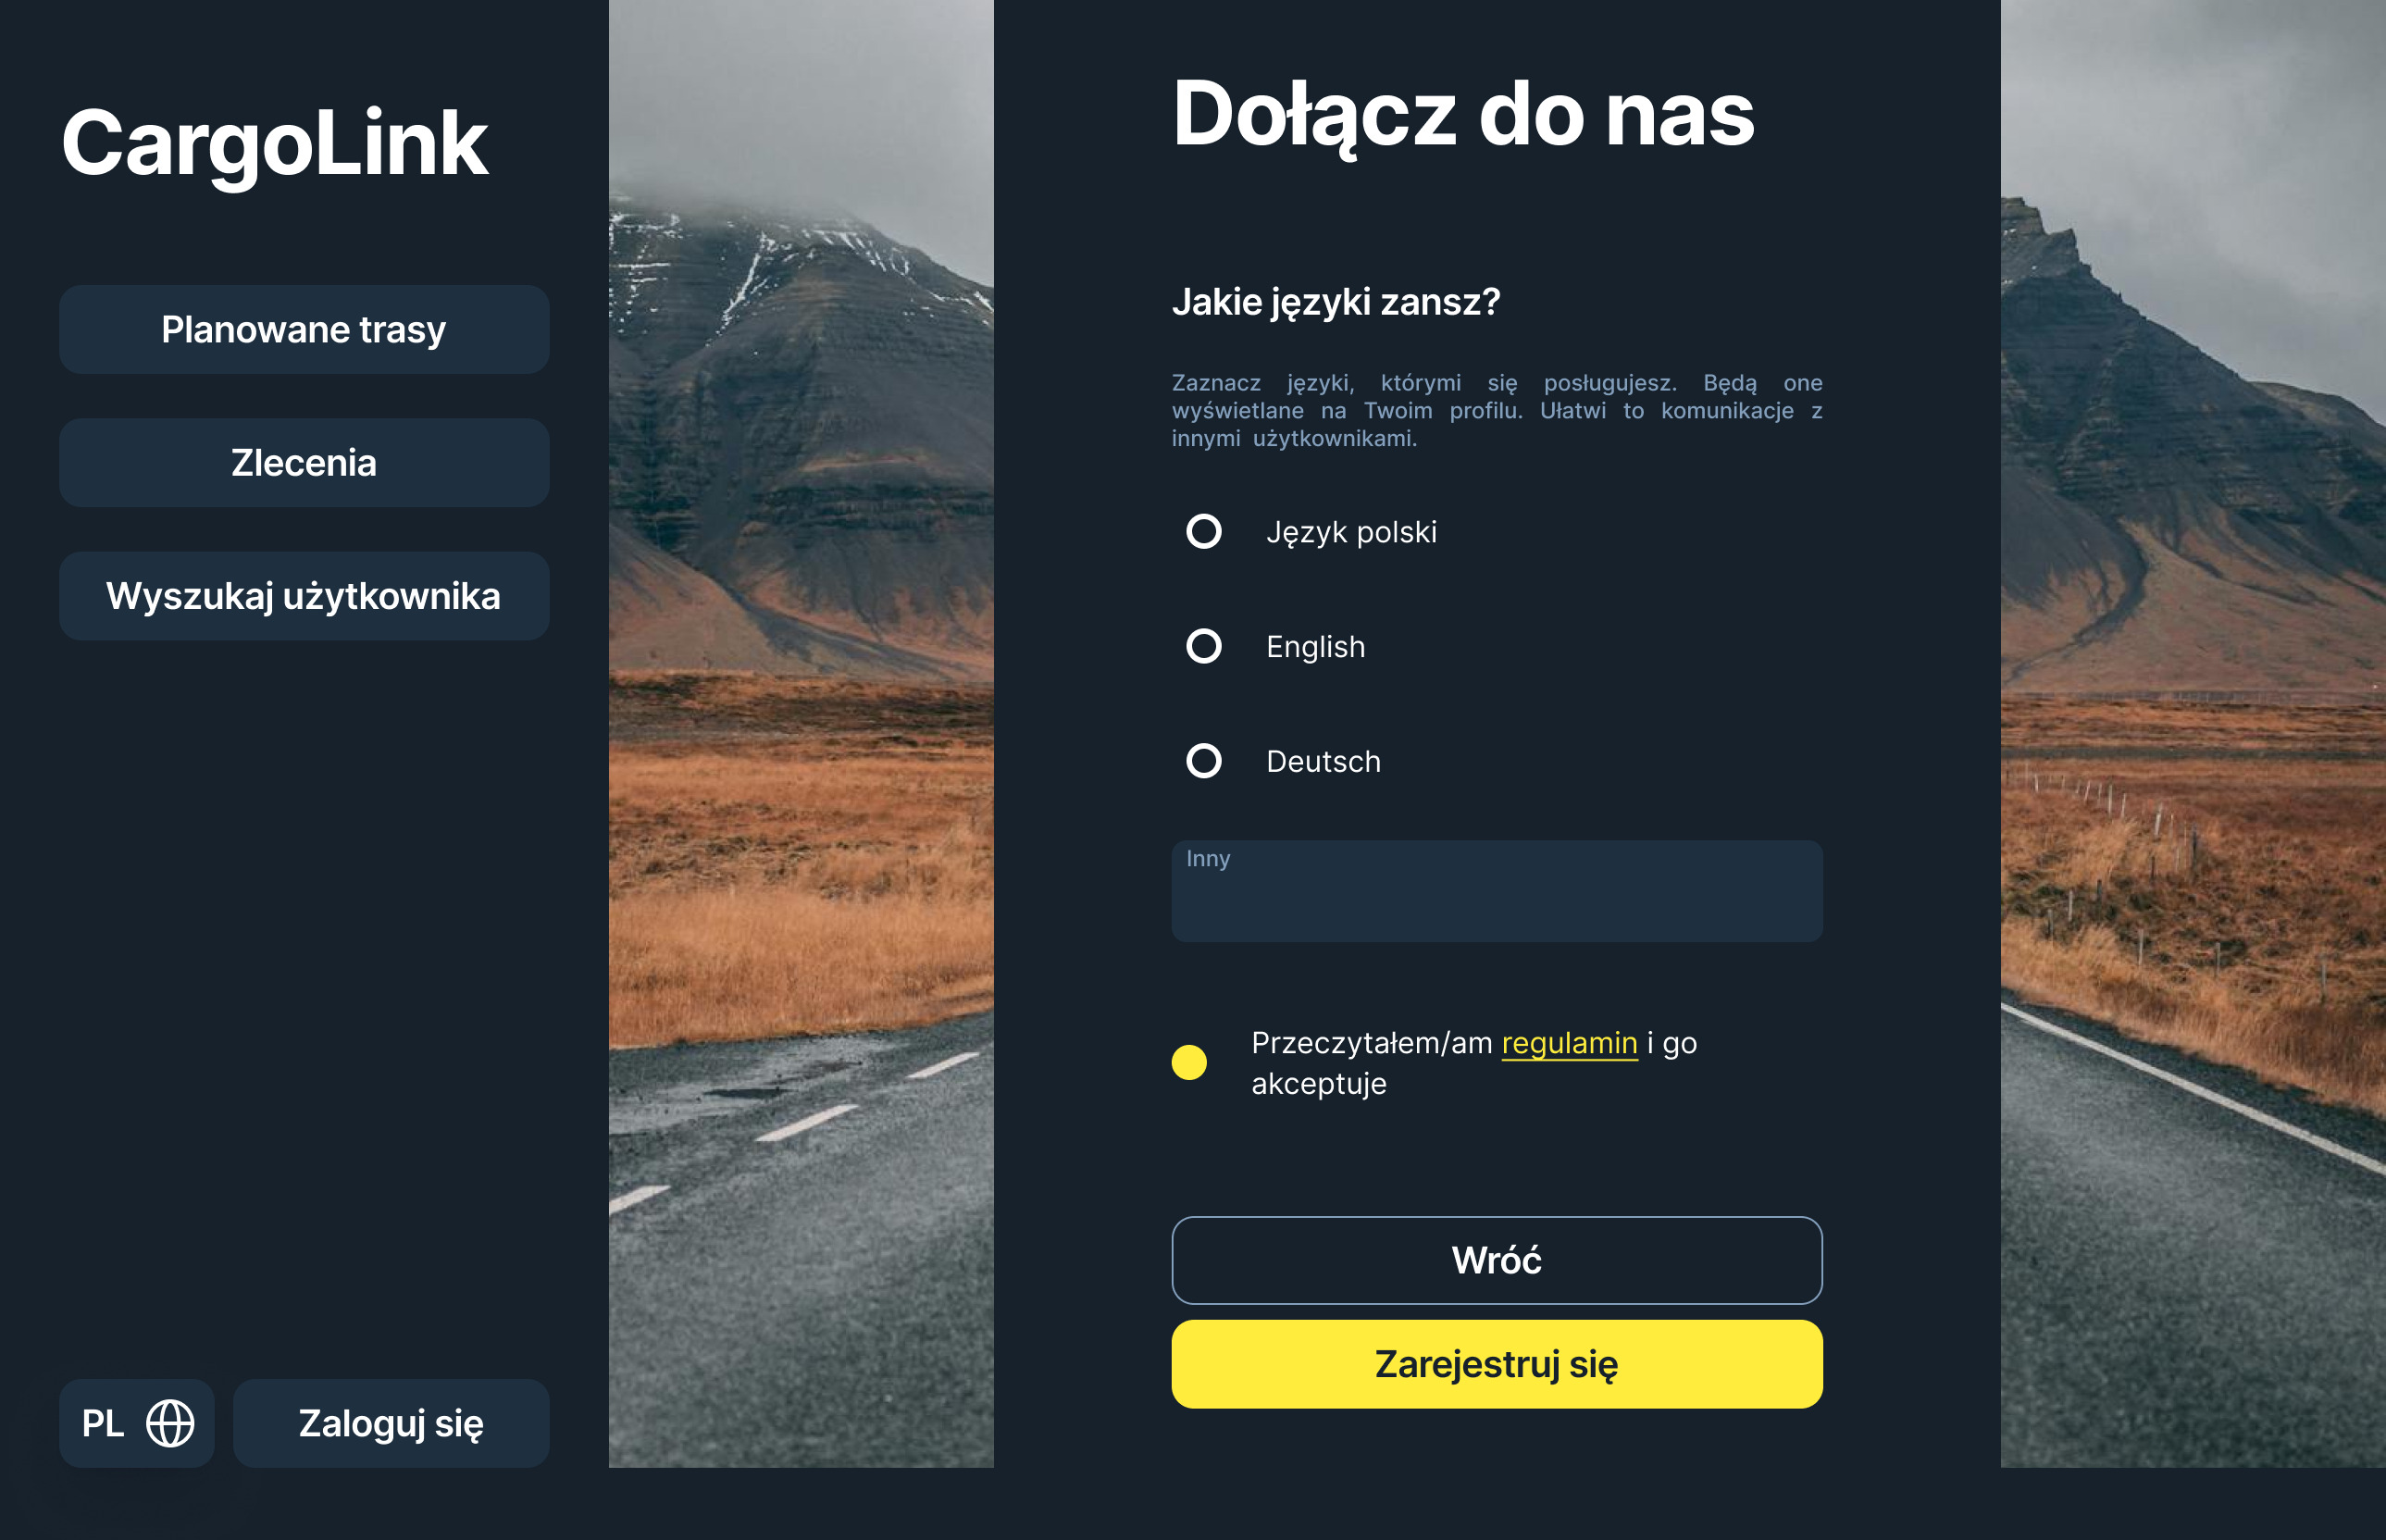
\includegraphics[width=0.45\textwidth]{rozdzial1/wybor_3_d.jpg}
  \end{tabular}
 \caption{Formularz rejestracji w wersji desktopowej: a) Wybór reprezentacji konta, b) Wybór języków, którymi użytkownik się posługuje, }
 \label{fig:Formularz rejestracji - ab2 - desktop}
\end{figure}

\texttt{Logowanie} \\
Zdarzenie inicjujące: Wpisanie danych logowania oraz kliknięcie przycisku \texttt{Zaloguj się}. \\
Warunki początkowe: Użytkownik nie jest zalogowany. \\
Przebieg podstawowy realizacji przypadku użycia:
\begin{enumerate}
    \item Wpisanie danych, email oraz hasło:
    \item Kliknięcie przycisku \texttt{Zaloguj się}; (Rys. \ref{fig:Formularz rejestracji - abc - mobile}.a lub \ref{fig:Formularz rejestracji - ab - desktop}.a)
    \item System sprawdza w bazie danych czy istnieje już użytkownik o podanym emailu oraz czy wprowadzone hasło jest prawidłowe;
    \item Zalogowanie użytkownika;
    \item Przejście do wyszukiwarki ogłoszeń o planowanych trasach, bądź zleceń (w zależności od wybranego typu konta).
\end{enumerate}
Przebieg alternatywny realizacji podpunktu (3a): W bazie danych nie znajduję się użytkownik o podanym emailu oraz haśle. System informuje o niepowodzeniu. \\
Warunki końcowe: W zależności od typu konta, przenosi do odpowiedniego miejsca w serwisie.\\

\texttt{Zmiana wersji językowej aplikacji} \\
Zdarzenie inicjujące: Wersja mobilna aplikacji - kliknięcie w trzy poziome kreski w nagłówku, aby otworzyć menu (np. Rys. \ref{fig:Formularz rejestracji - abc - mobile}.a). Wersja desktopowa aplikacji - kliknięcie przycisku z ikoną globu (np. Rys. \ref{fig:Formularz rejestracji - ab - desktop}.a). \\
Warunki początkowe: Brak. \\
Przebieg podstawowy realizacji przypadku użycia:
\begin{enumerate}
    \item Jeżeli w wersji mobilnej - kliknięcie w trzy poziome kreski w nagłówku, aby otworzyć menu (np. Rys. \ref{fig:Formularz rejestracji - abc - mobile}.a);
    \item Kliknięcie przycisku z ikoną globu (Rys. \ref{Rys. fig:Menu nawigacji po aplikacji - ab}.a lub np. Rys. \ref{fig:Formularz rejestracji - c - desktop});
    \item Wybranie jednego z trzech języków z menu (Rys. \ref{Rys. fig:Menu nawigacji po aplikacji - ab}.b lub Rys. \ref{Rys. fig:Wybór języka aplikacji - desktop});
    \item Zmienienie języka w jakim wyświetlana jest aplikacja;
\end{enumerate}
\begin{figure}[H]
	\centering
        \begin{tabular}{@{}ccc@{}}
            a) & b)\\
		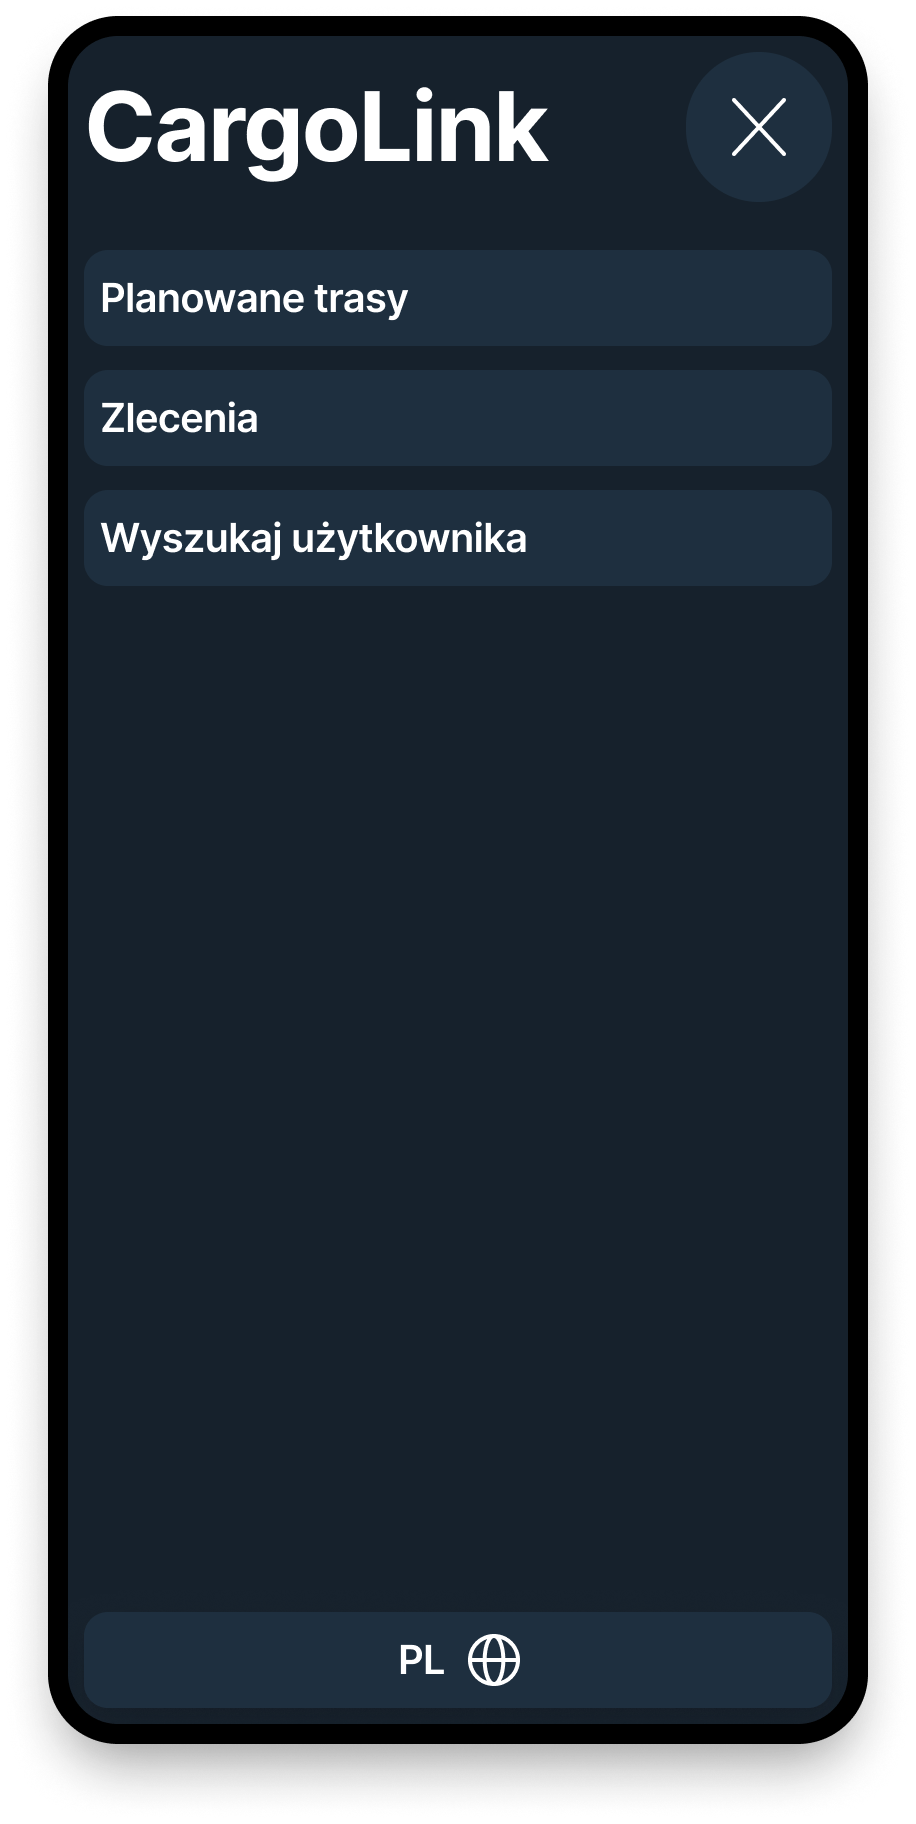
\includegraphics[width=0.3\linewidth]{rozdzial1/menu_m.png} &
		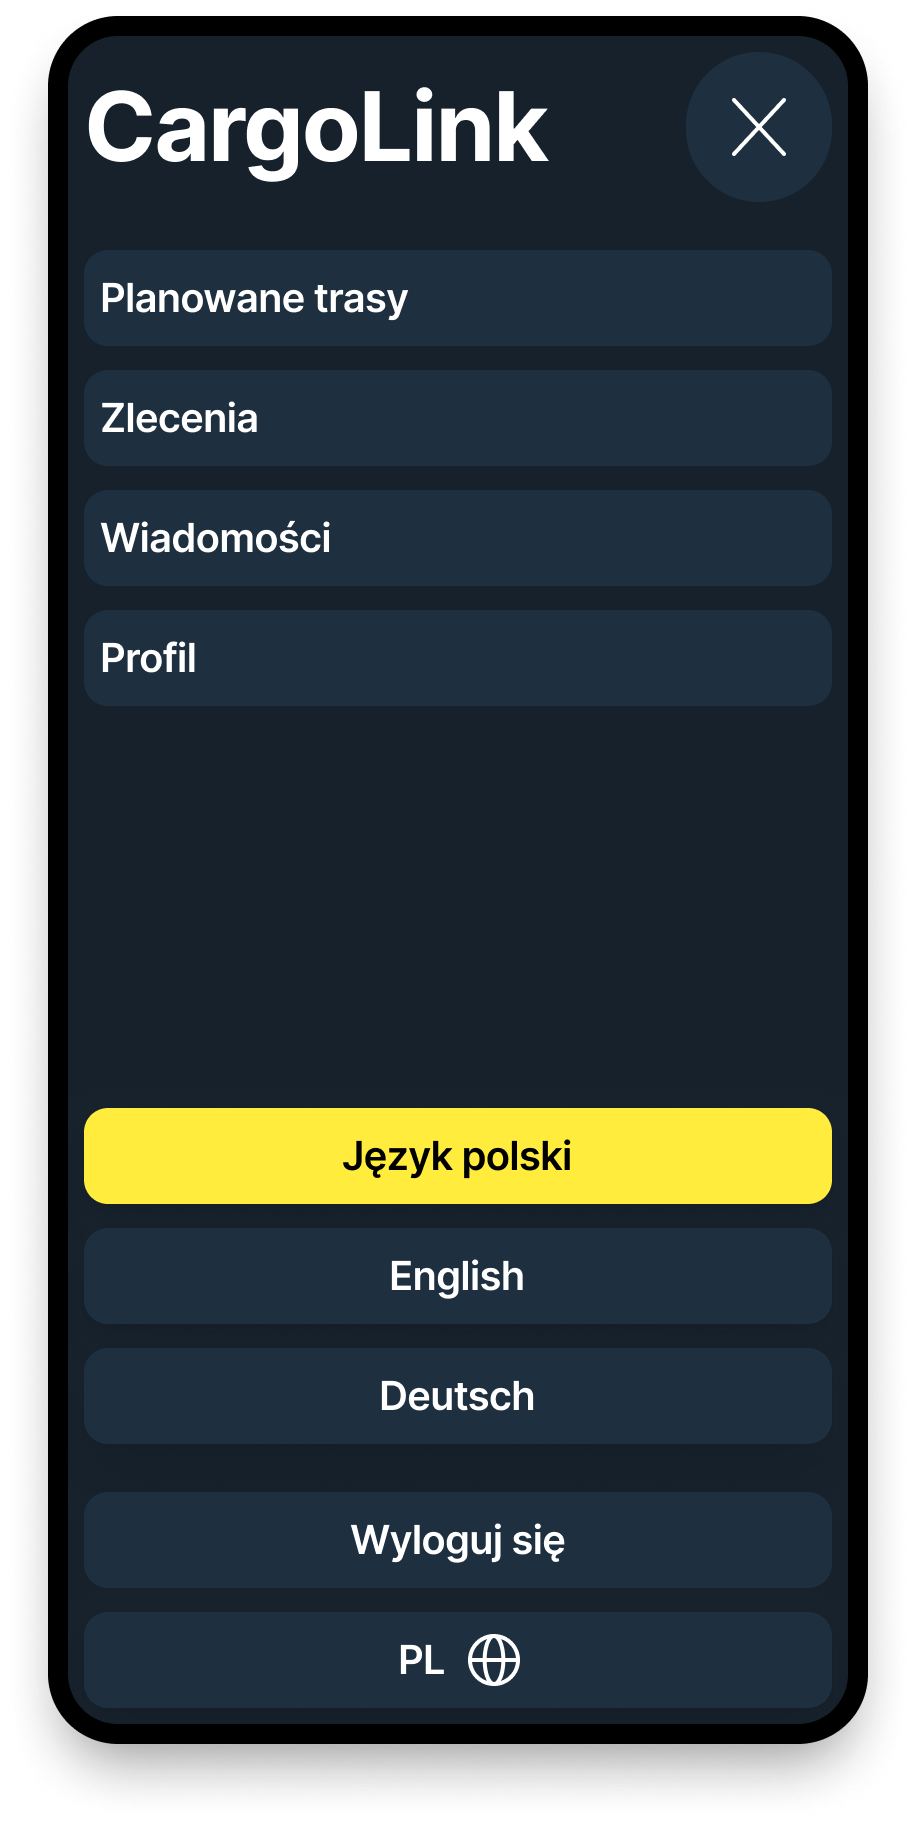
\includegraphics[width=0.3\linewidth]{rozdzial1/menu_język_m.png}
		\end{tabular}
	\caption{Menu nawigacji po aplikacji w wersji mobilnej: a) Menu nawigacji, b) Menu nawigacji z klikniętym przyciskiem wyboru języka}
	\label{Rys. fig:Menu nawigacji po aplikacji - ab}
\end{figure}
\begin{figure}[H]
 \centering
  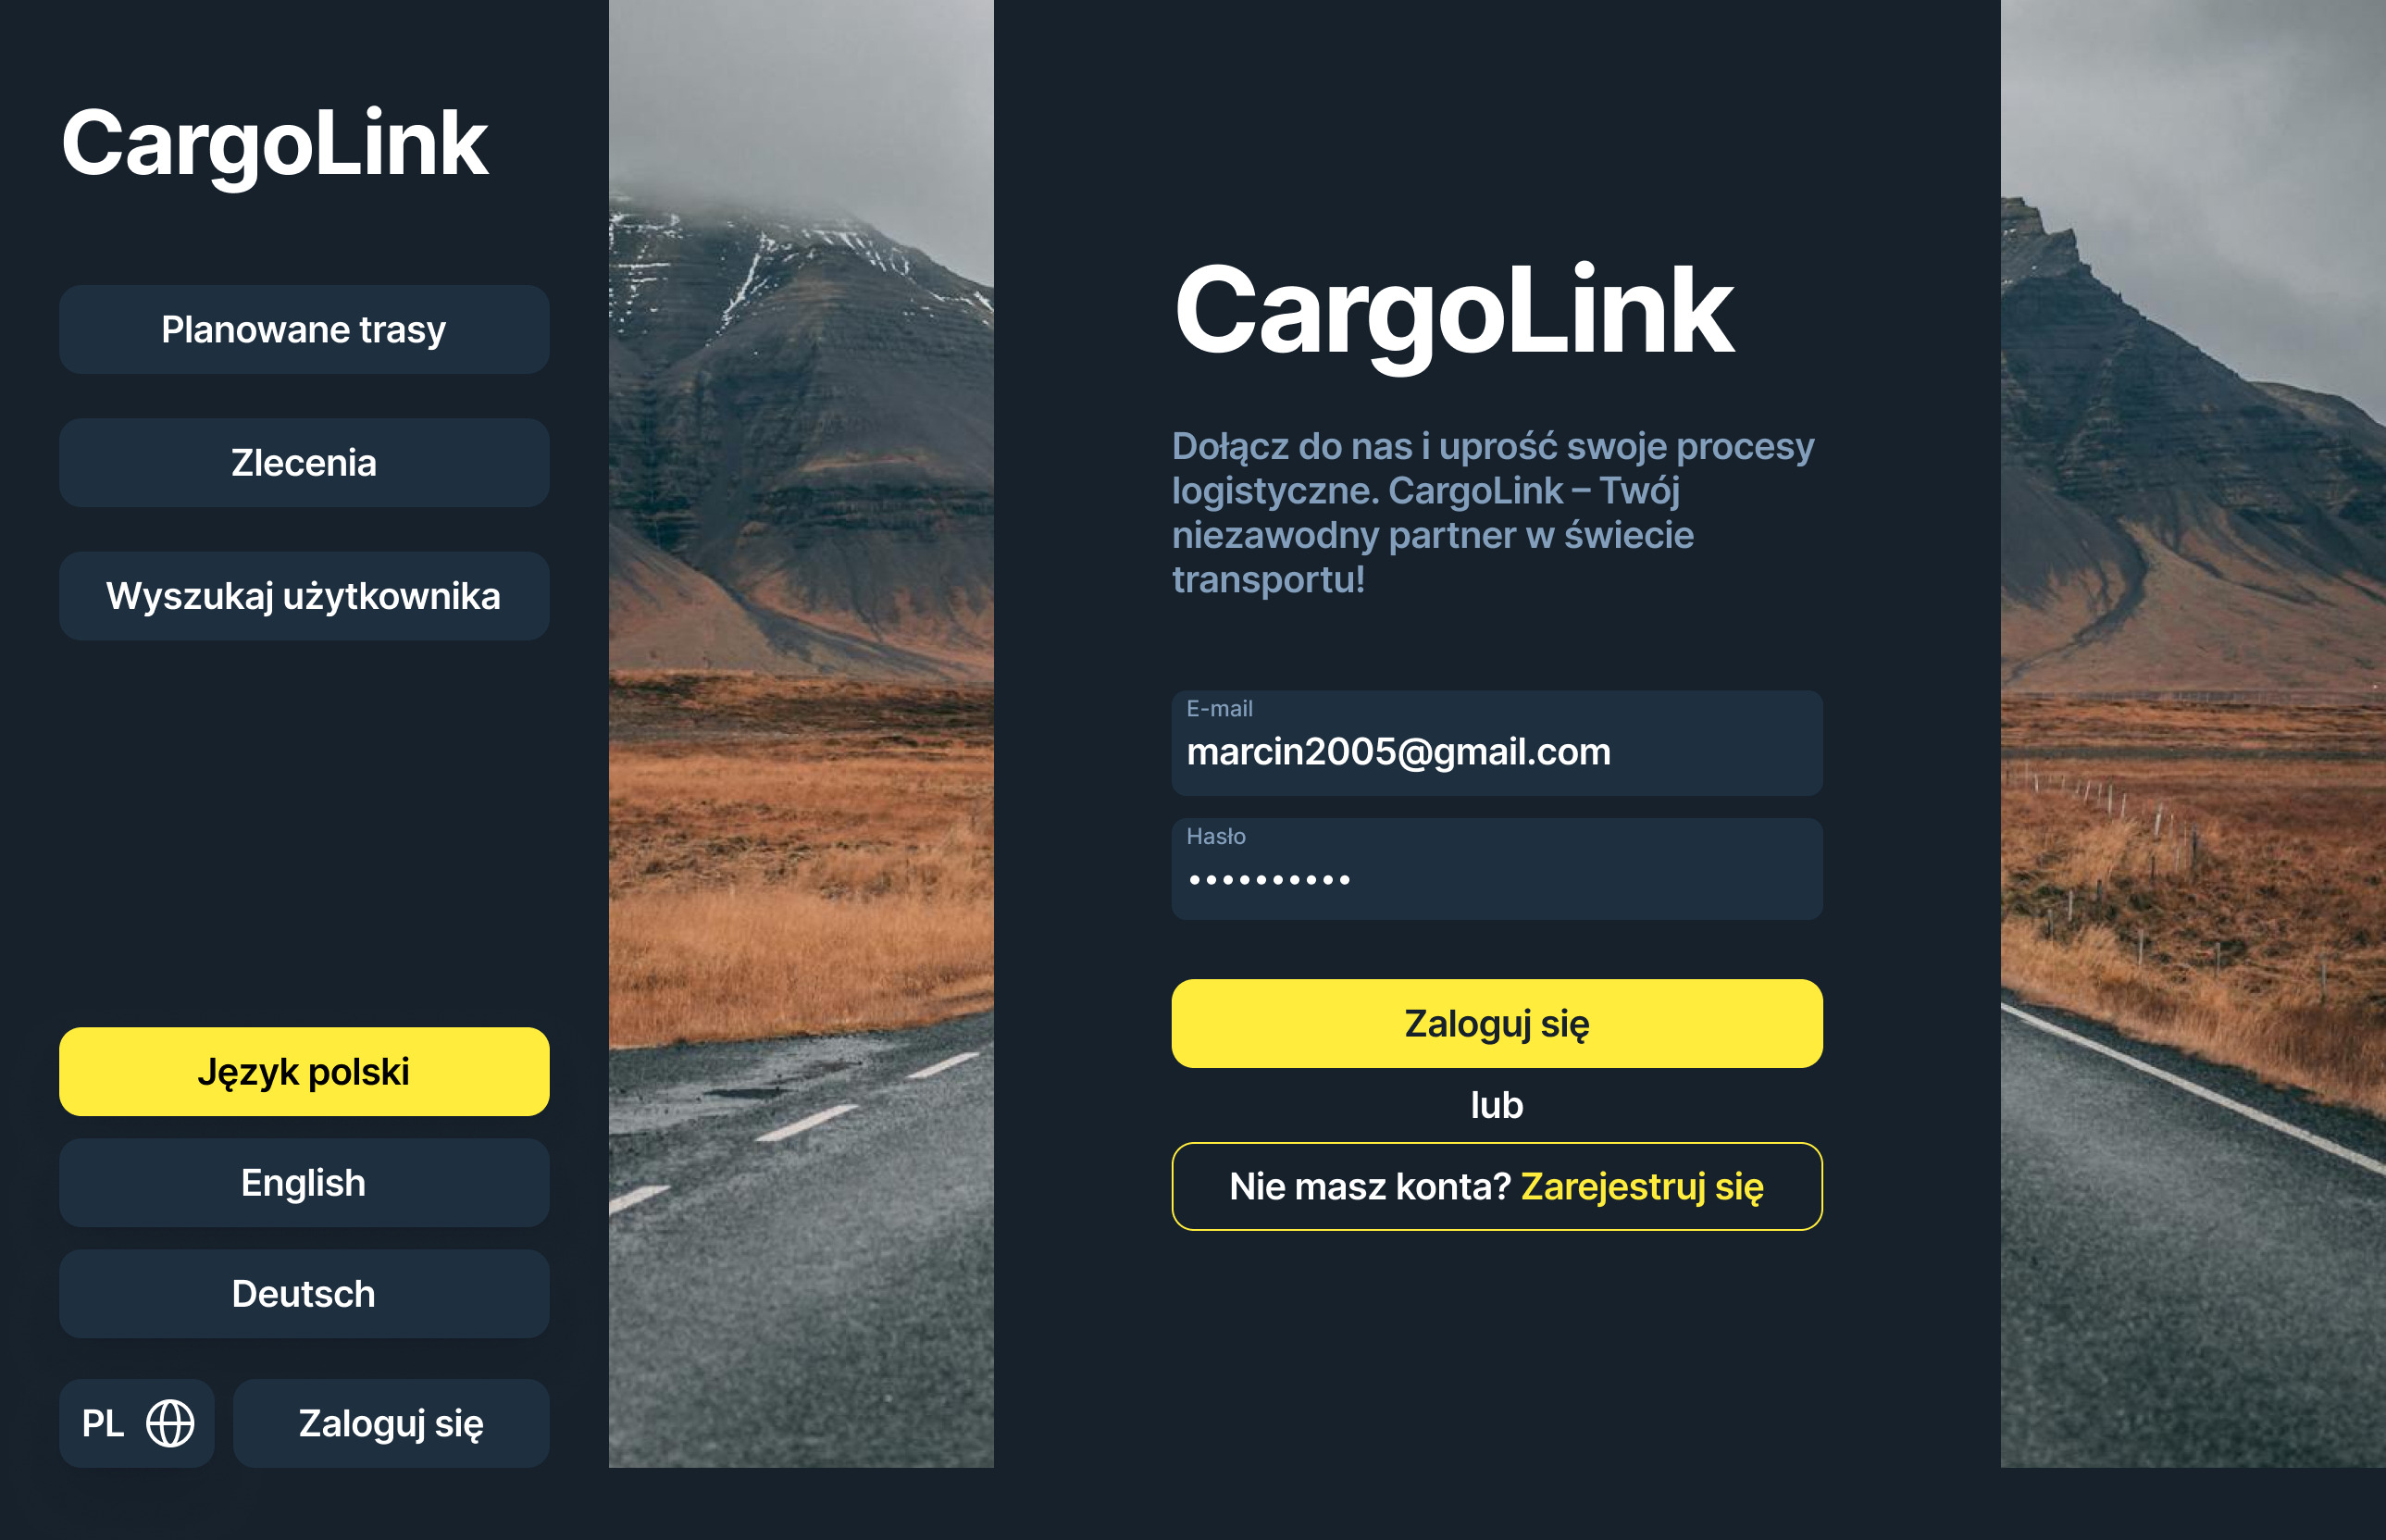
\includegraphics[width=0.7\textwidth]{rozdzial1/menu_jezyk_d.jpg}
 \caption{Menu wyboru języka aplikacji w wersji desktopowej}
 \label{Rys. fig:Wybór języka aplikacji - desktop}
\end{figure}

\texttt{Wyszukiwanie użytkowników} \\
Zdarzenie inicjujące: Wersja mobilna aplikacji - kliknięcie w trzy poziome kreski w nagłówku, aby otworzyć menu (np. Rys. \ref{fig:Formularz rejestracji - abc - mobile}.a). Wersja desktopowa aplikacji - kliknięcie przycisku \texttt{Wyszukaj użytkownika} (np. Rys. \ref{fig:Formularz rejestracji - ab - desktop}.a). \\
Warunki początkowe: Brak. \\
Przebieg podstawowy realizacji przypadku użycia:
\begin{enumerate}
    \item Jeżeli w wersji mobilnej - kliknięcie w trzy poziome kreski w nagłówku, aby otworzyć menu (np. Rys. \ref{fig:Formularz rejestracji - abc - mobile}.a);
    \item Kliknięcie przycisku \texttt{Wyszukaj użytkownika} (Rys. \ref{Rys. fig:Menu nawigacji po aplikacji - ab}.a lub \ref{fig:Formularz rejestracji - ab - desktop}.a);
    \item Wpisanie danych szukanego użytkownika, takich jak imię, nazwisko, e-mail lub typ konta (Rys. \ref{Rys. fig:Wyszukiwanie użytkownika - mobile} lub \ref{Rys. fig:Wyszukiwanie użytkownika - destkop});
    \item Kliknięcie przycisku \texttt{Szukaj} (Rys. \ref{Rys. fig:Wyszukiwanie użytkownika - mobile} lub \ref{Rys. fig:Wyszukiwanie użytkownika - destkop});
    \item Wyświetlenie wszystkich użytkowników spełniających podane kryteria.
\end{enumerate}
Warunki końcowe: Serwis zwraca wszystkie profile spełniające wpisane wymagania.\\
\begin{figure}[H]
	\centering
		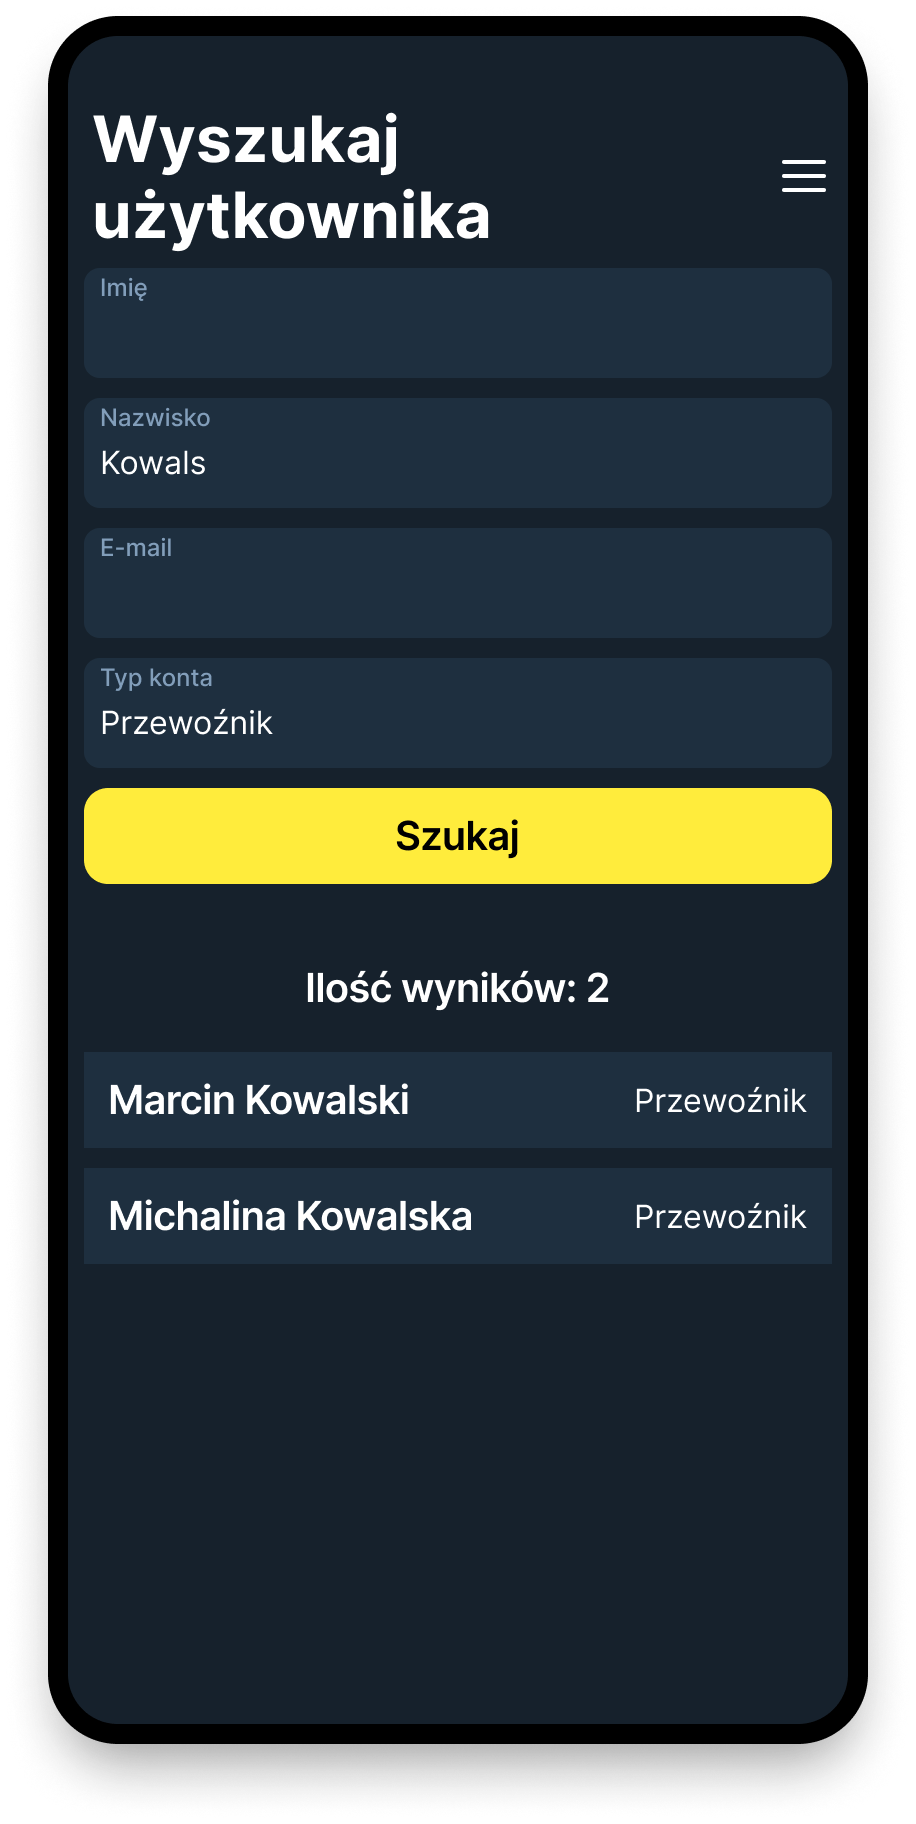
\includegraphics[width=0.3\linewidth]{rozdzial1/szukaj_uzytkownika_m.png}
	\caption{Wyszukiwanie użytkownika w wersji mobilnej}
	\label{Rys. fig:Wyszukiwanie użytkownika - mobile}
\end{figure}
\begin{figure}[H]
	\centering
		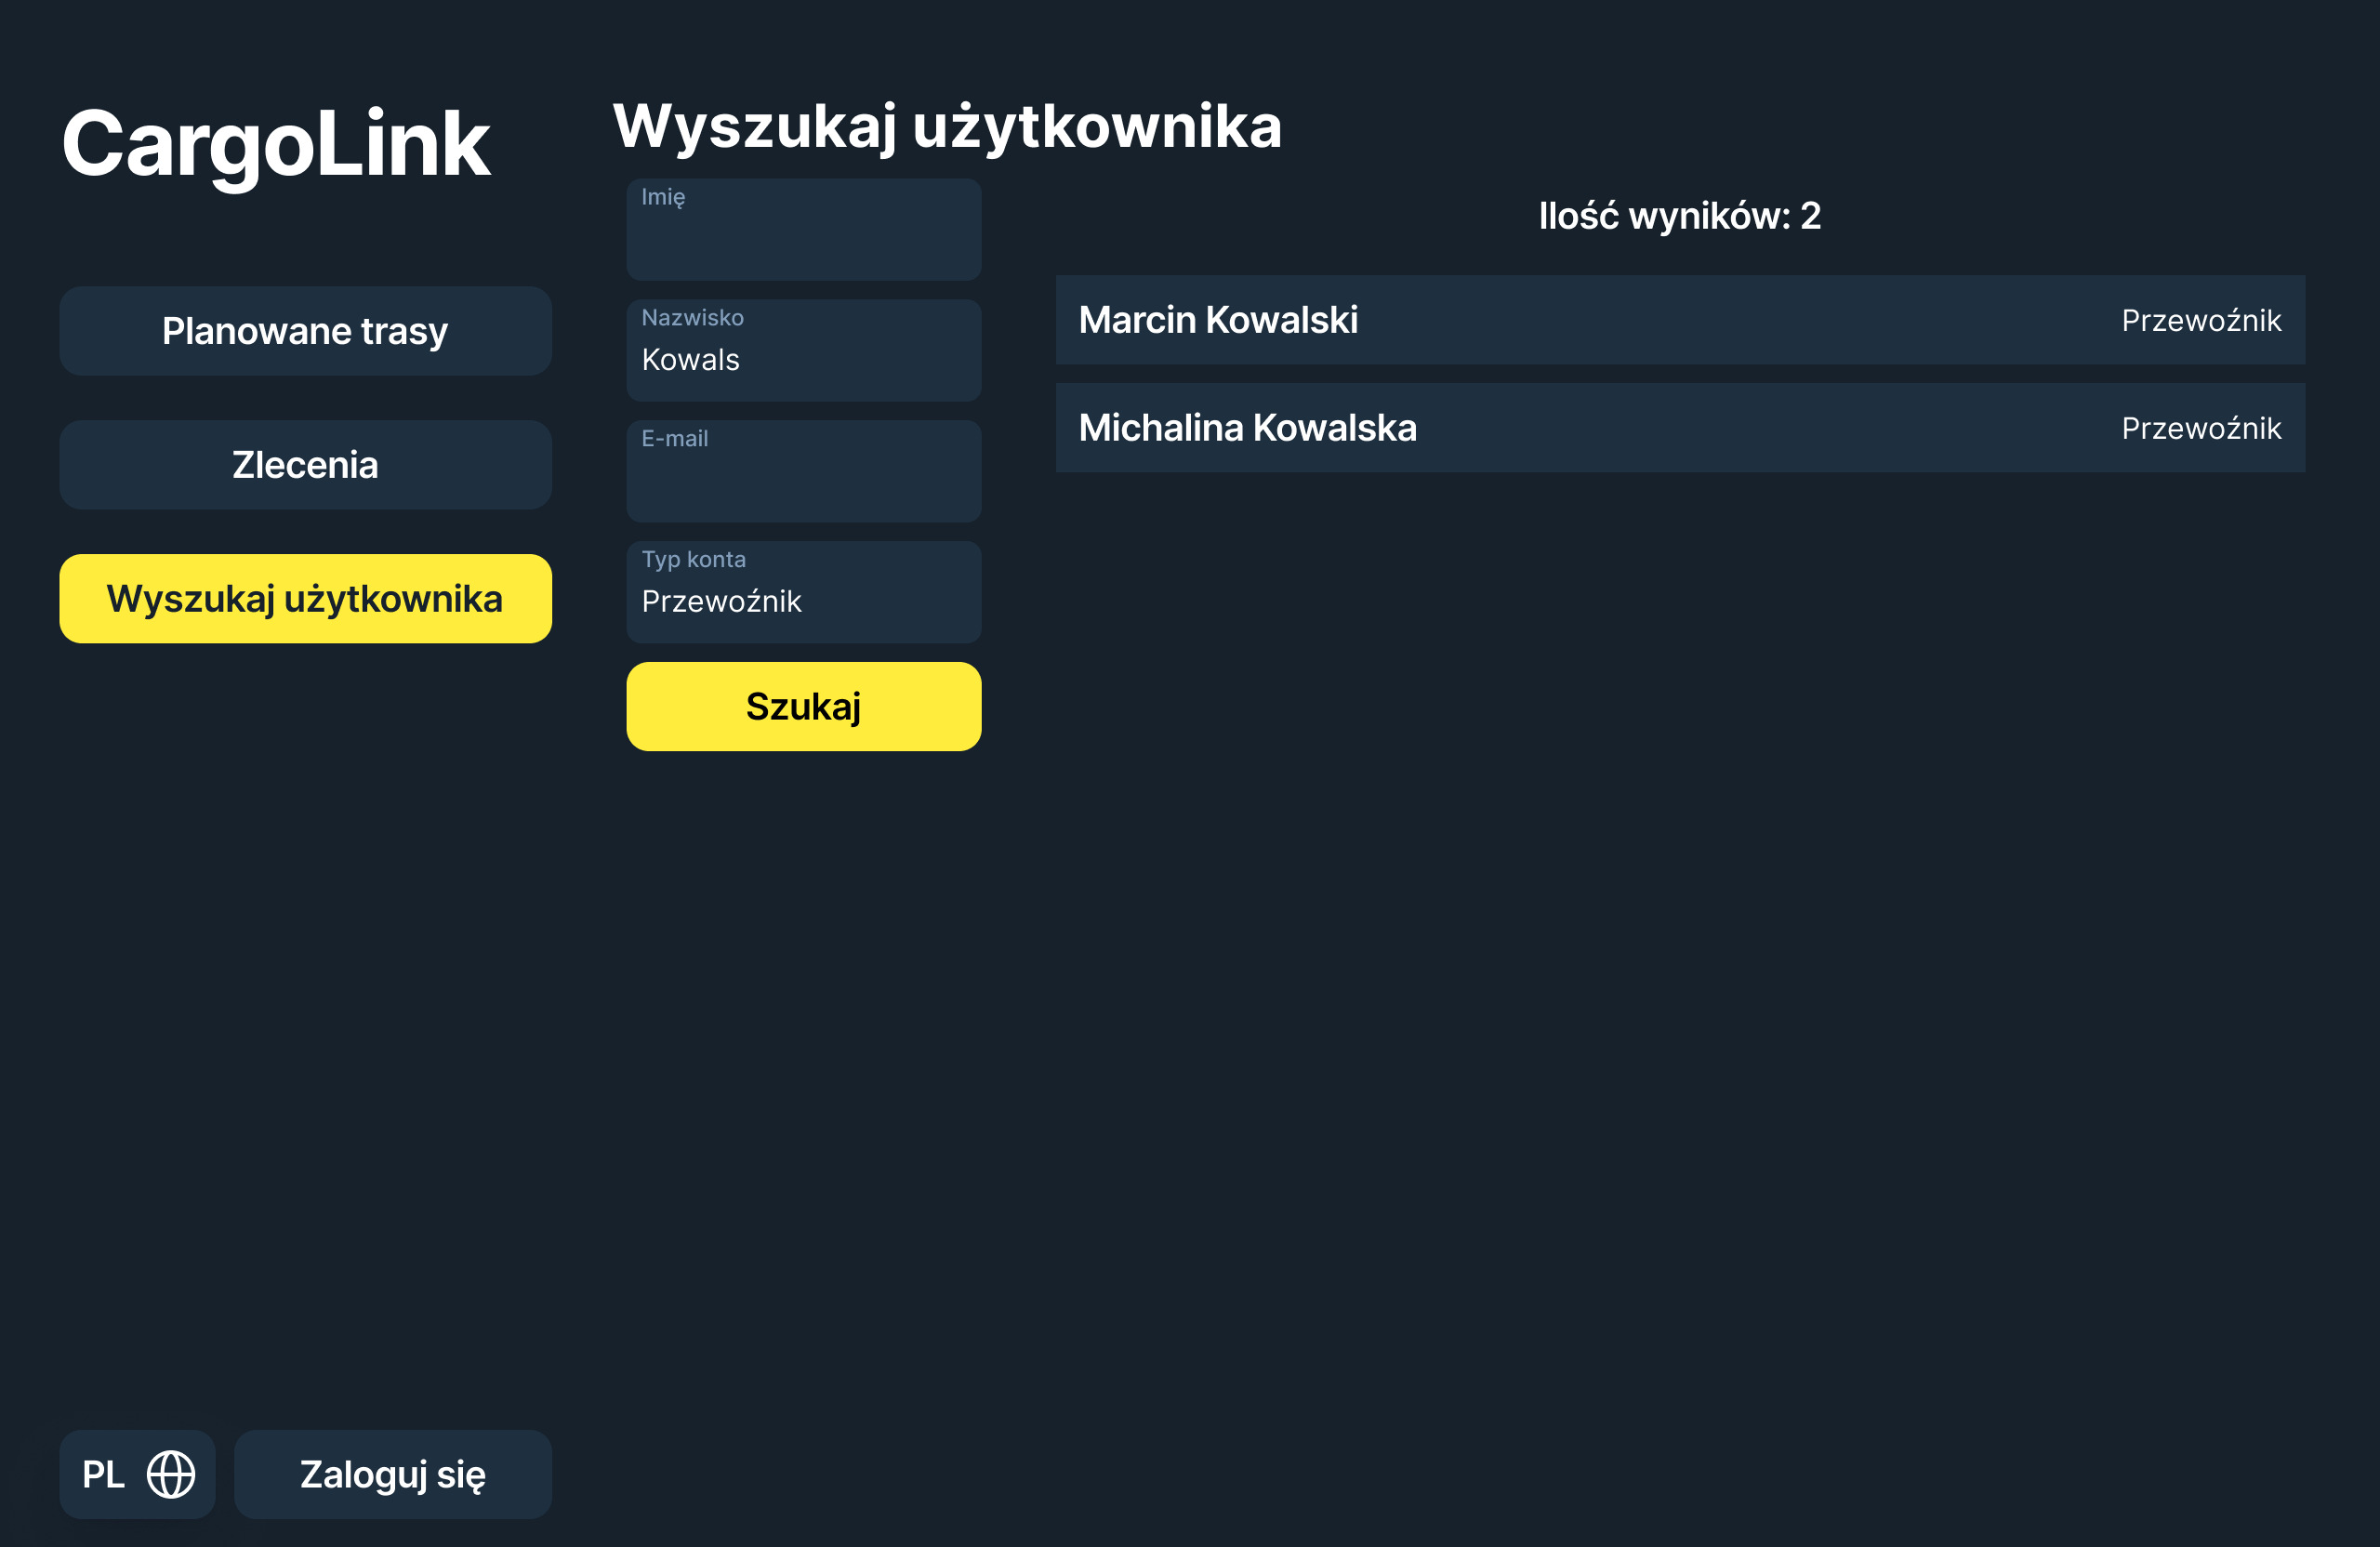
\includegraphics[width=0.7\linewidth]{rozdzial1/szukaj_uzytkownika_d.jpg}
	\caption{Wyszukiwanie użytkownika w wersji desktopowej}
	\label{Rys. fig:Wyszukiwanie użytkownika - destkop}
\end{figure}

\label{Przeglądanie zleceń}
\texttt{Przeglądanie zleceń} \\
Zdarzenie inicjujące: Wersja mobilna aplikacji - kliknięcie w trzy poziome kreski w nagłówku, aby otworzyć menu (np. Rys. \ref{fig:Formularz rejestracji - abc - mobile}.a). Wersja desktopowa aplikacji - kliknięcie przycisku \texttt{Zlecenia} (np. Rys. \ref{fig:Formularz rejestracji - ab - desktop}.a). \\
Warunki początkowe: Brak. \\
Przebieg podstawowy realizacji przypadku użycia:
\begin{enumerate}
    \item Jeżeli w wersji mobilnej - kliknięcie w trzy poziome kreski w nagłówku, aby otworzyć menu (np. Rys. \ref{fig:Formularz rejestracji - abc - mobile}.a);
    \item Kliknięcie przycisku \texttt{Zlecenia} (Rys. \ref{Rys. fig:Menu nawigacji po aplikacji - ab}.a lub \ref{fig:Formularz rejestracji - ab - desktop}.a);
    \item Wyświetlenie listy ogłoszeń dodanych przez zleceniodawców.
\end{enumerate}
Warunki końcowe: Wyświetlenie przeglądarki zleceń. (Rys. \ref{Rys. fig:Przeglądarka zleceń i planowanych tras - ab - mobile}.a lub \ref{Rys. fig:Przeglądarka zleceń i planowanych tras - ab - desktop}.a)
\begin{figure}[H]
	\centering
	\begin{tabular}{@{}ccc@{}}
            a) & b)\\
    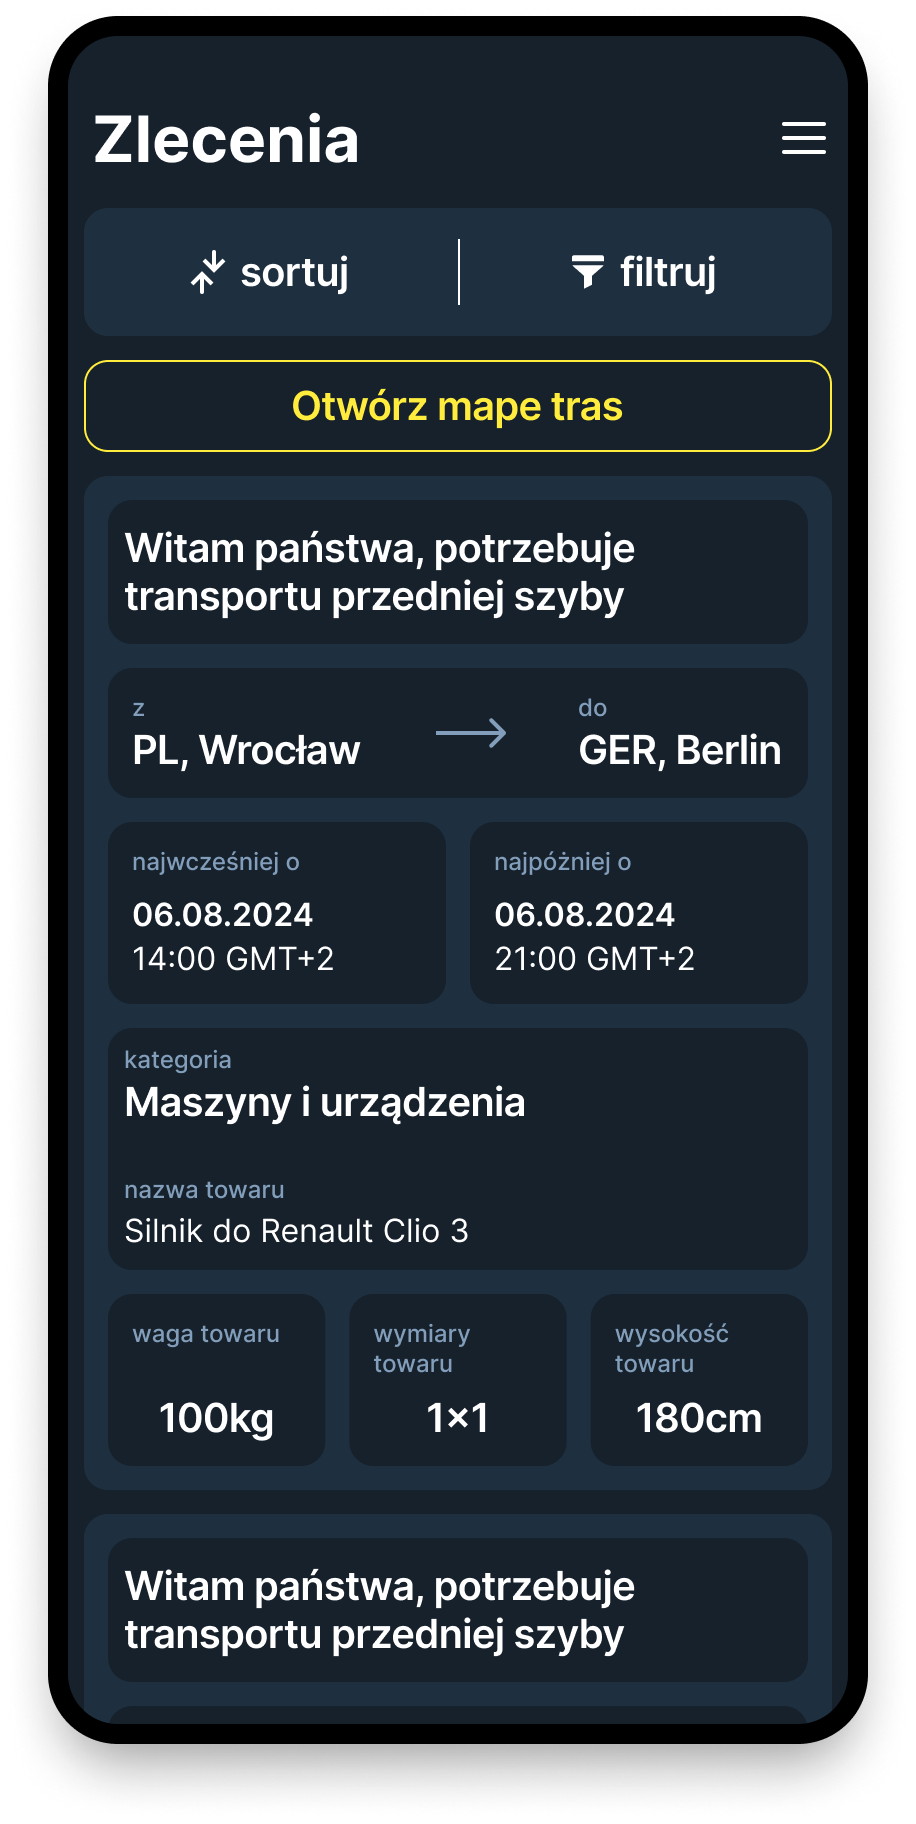
\includegraphics[width=0.3\linewidth]{rozdzial1/zlecenia_m.png} &
    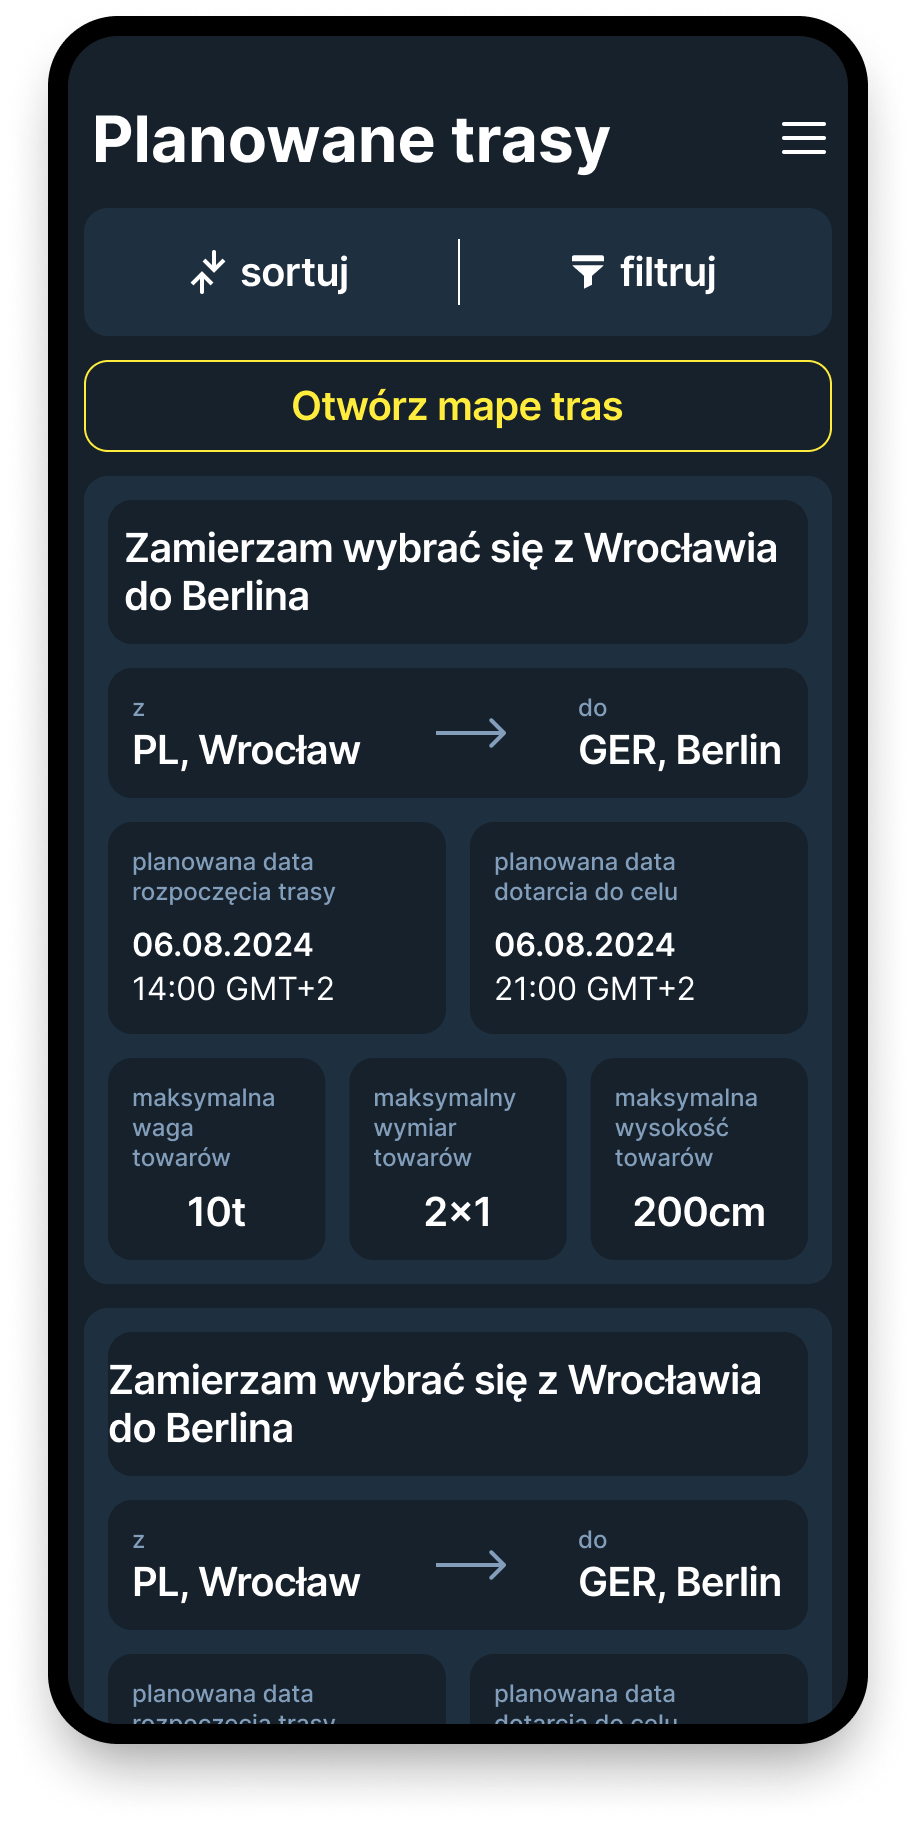
\includegraphics[width=0.3\linewidth]{rozdzial1/planowane_trasy_m.png}
    \end{tabular}
    \caption{Przeglądarka zleceń i planowanych tras w wersji mobilnej: a) Przeglądarka zleceń, b) Przeglądarka ogłoszeń planowanych tras}
	\label{Rys. fig:Przeglądarka zleceń i planowanych tras - ab - mobile}
\end{figure}
\begin{figure}[H]
 \centering
  \begin{tabular}{@{}ccc@{}}
  a) & b)\\
  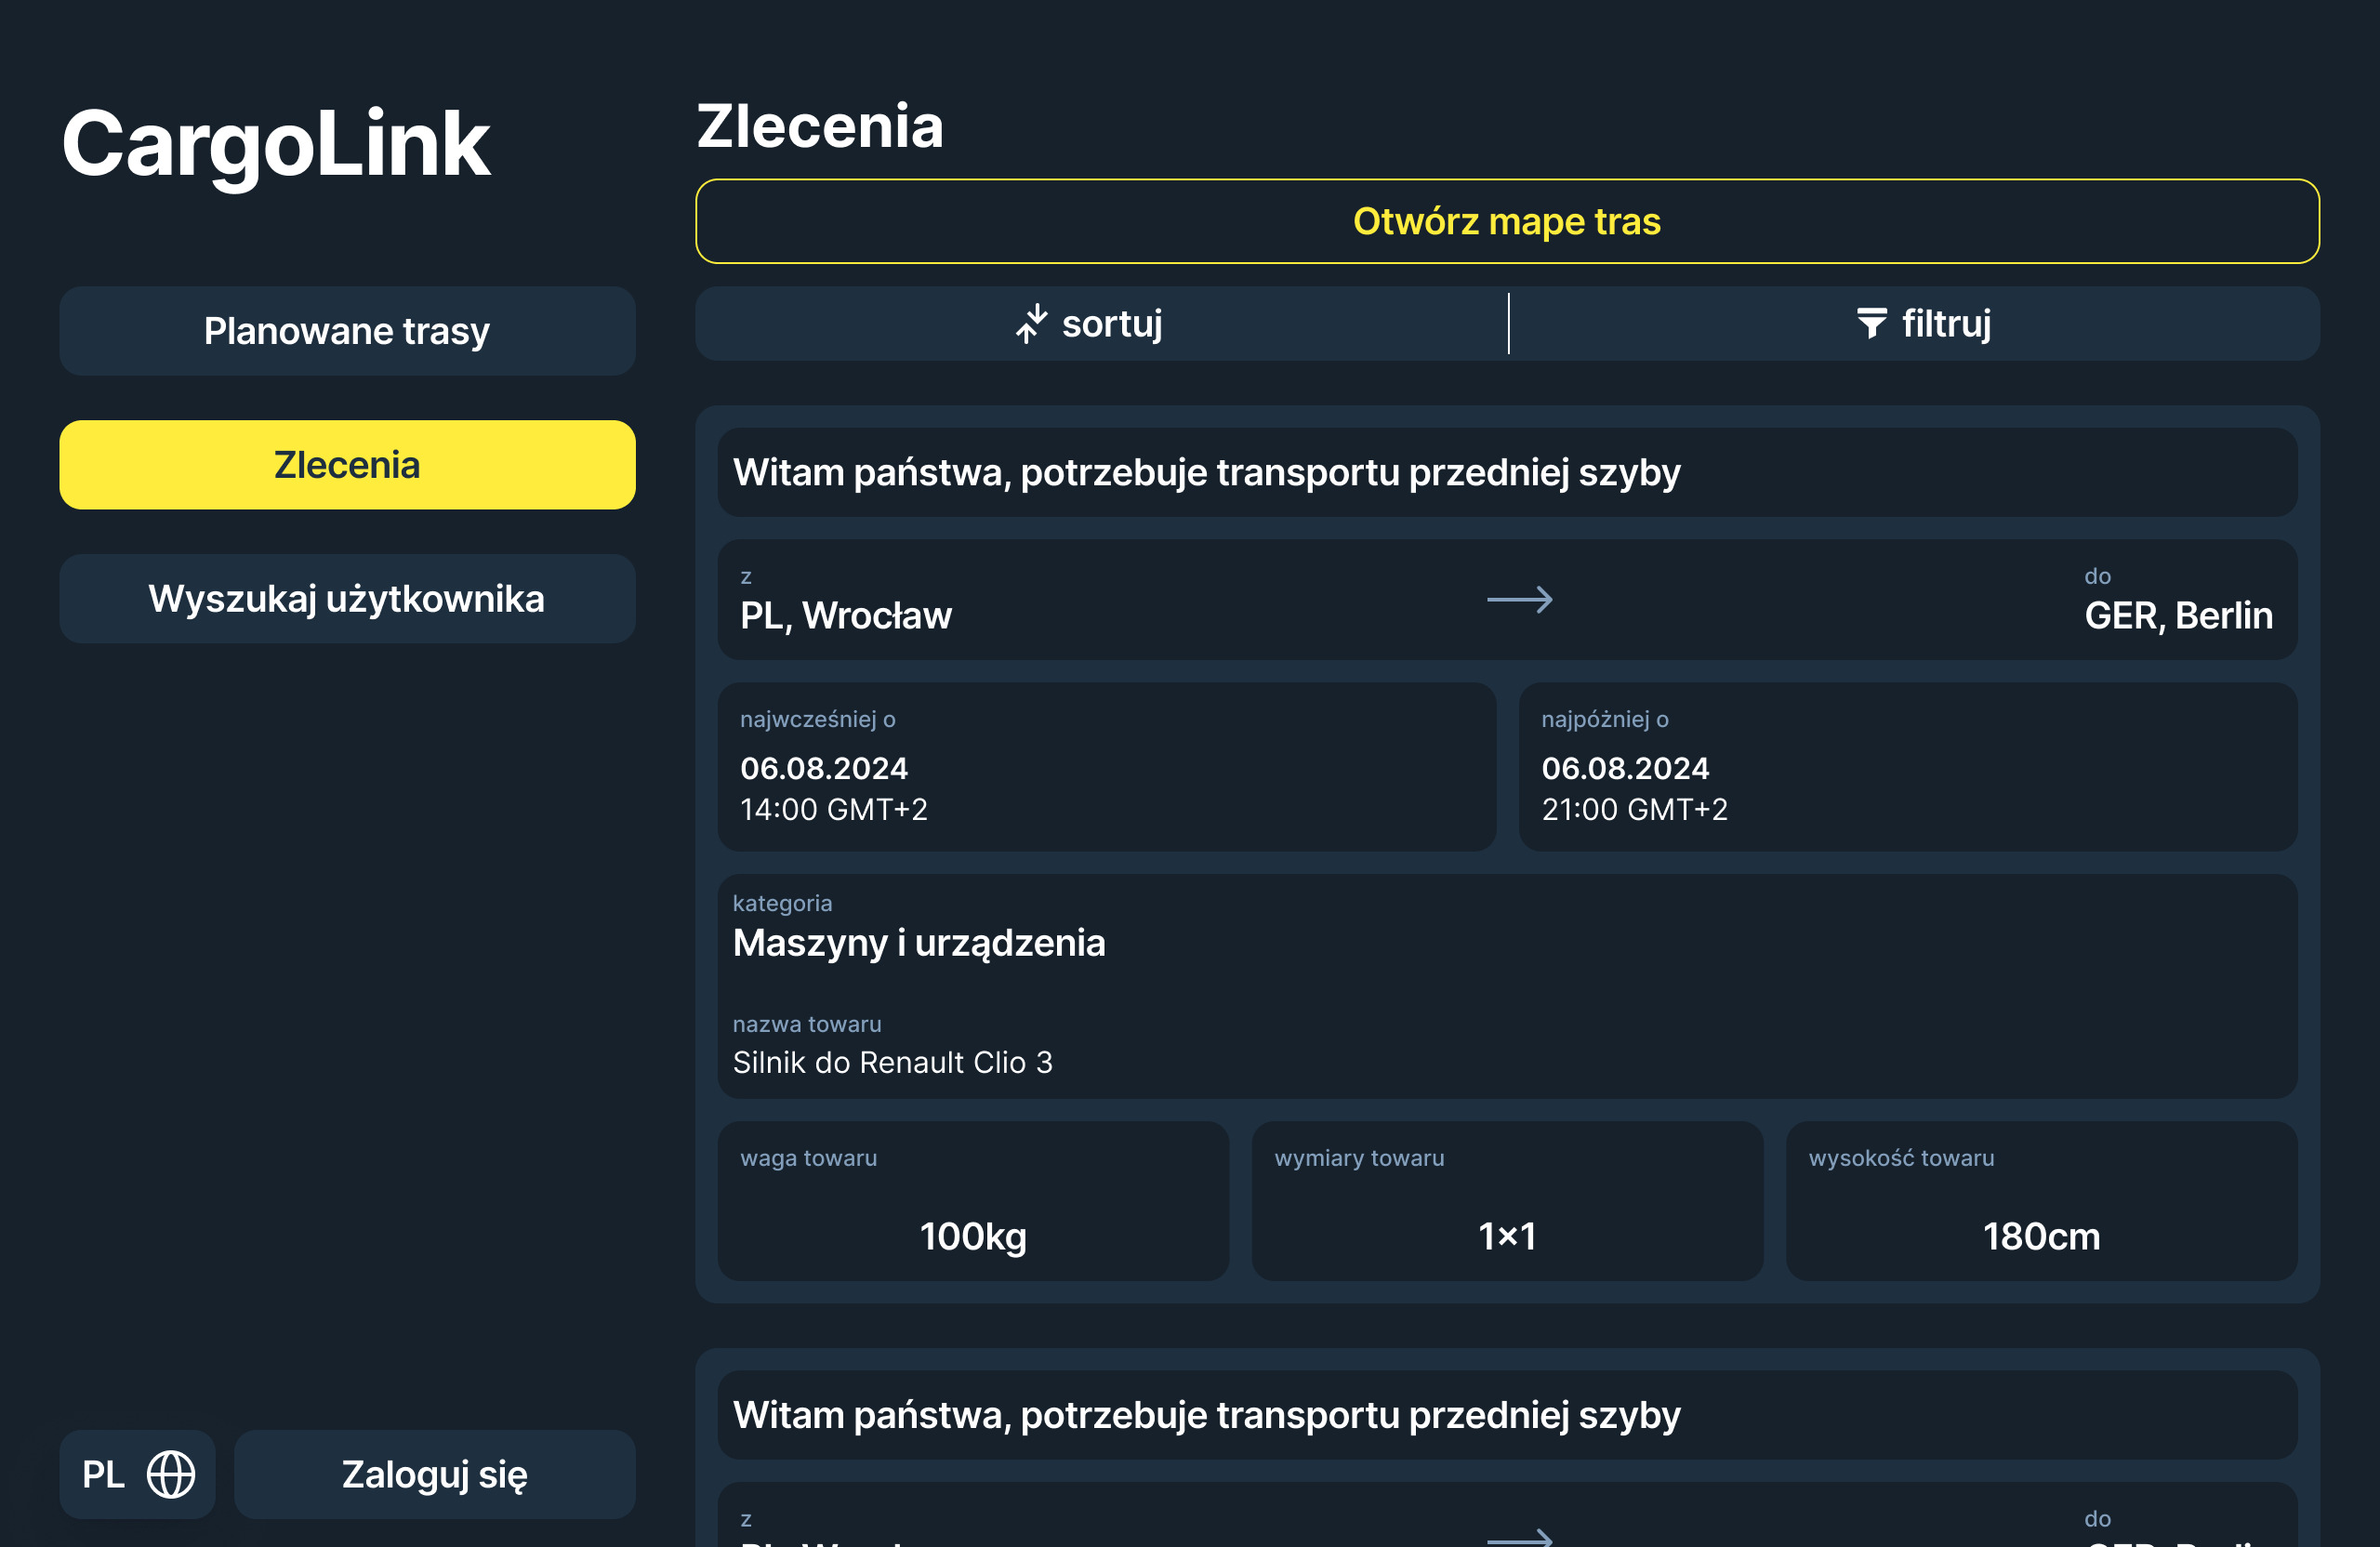
\includegraphics[width=0.45\textwidth]{rozdzial1/zlecenia_d.jpg} &
  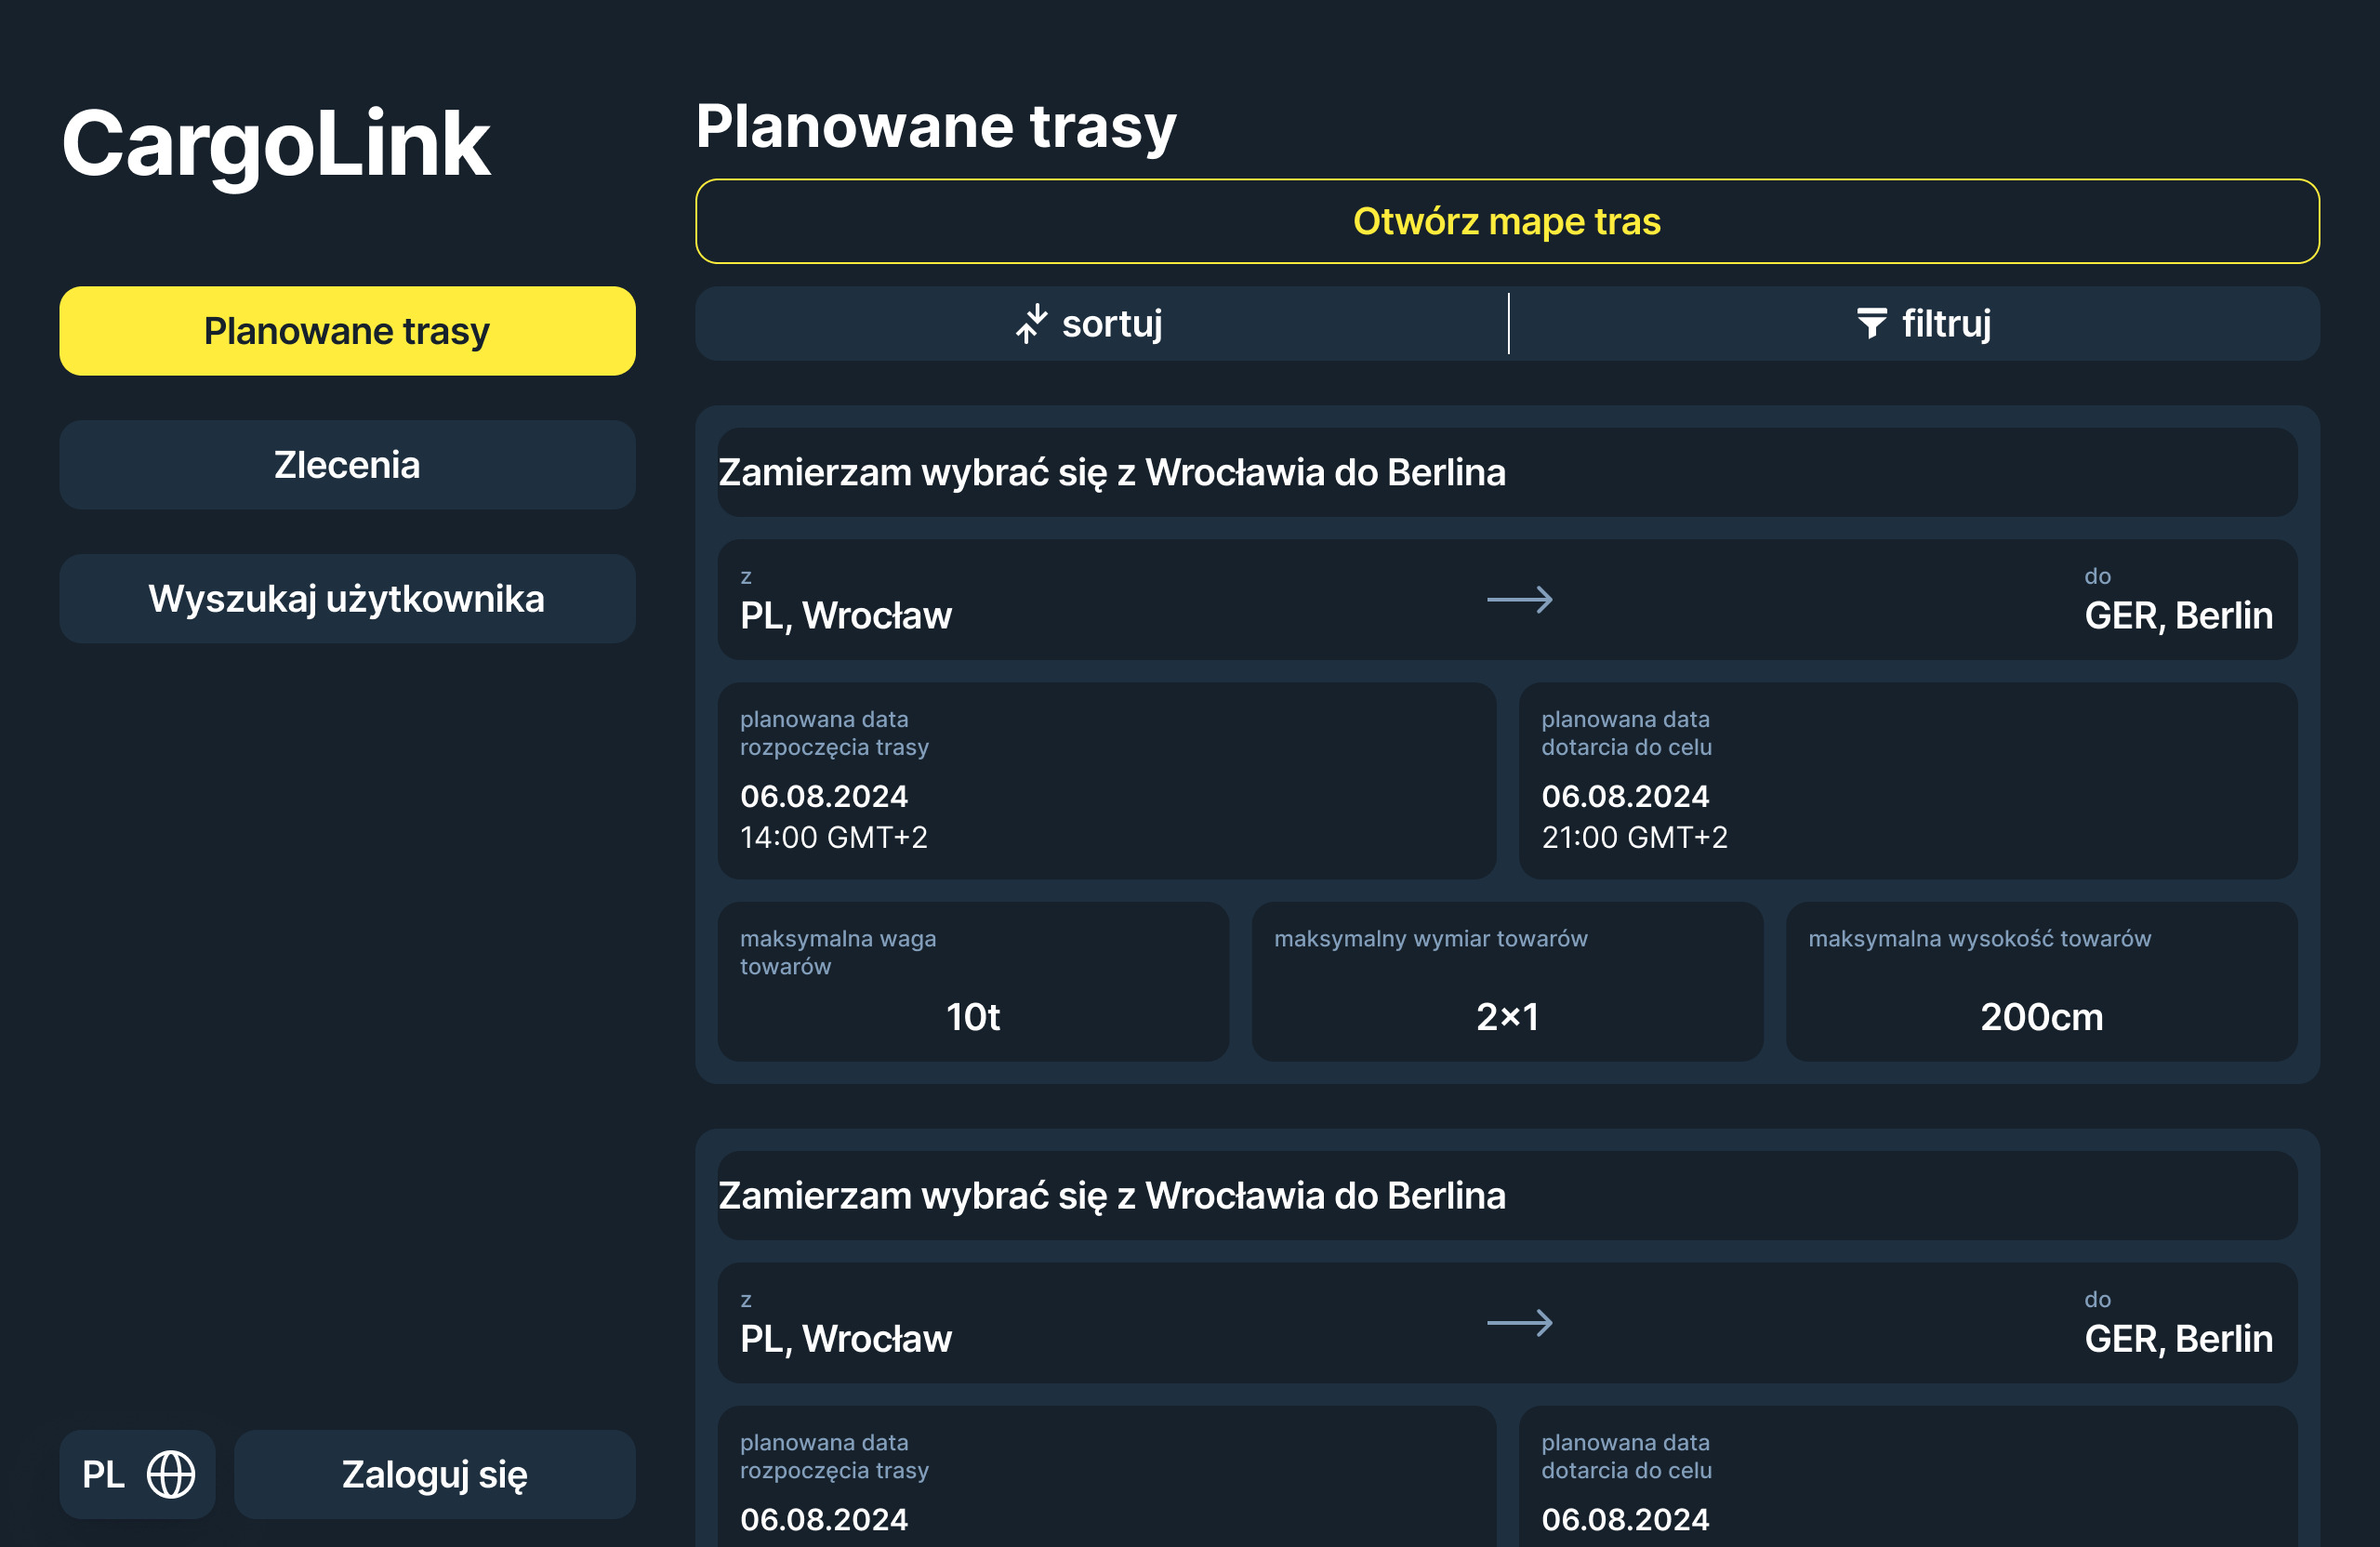
\includegraphics[width=0.45\textwidth]{rozdzial1/planowane_trasy_d.jpg}
  \end{tabular}
 \caption{Przeglądarka zleceń i planowanych tras w wersji desktopowej: a) Przeglądarka zleceń, b) Przeglądarka ogłoszeń planowanych tras}
 \label{Rys. fig:Przeglądarka zleceń i planowanych tras - ab - desktop}
\end{figure}

\label{Przeglądanie ogłoszeń planowanych tras}
\texttt{Przeglądanie ogłoszeń planowanych tras} \\
Zdarzenie inicjujące: Wersja mobilna aplikacji - kliknięcie w trzy poziome kreski w nagłówku, aby otworzyć menu (np. Rys. \ref{fig:Formularz rejestracji - abc - mobile}.a). Wersja desktopowa aplikacji - kliknięcie przycisku \texttt{Zlecenia} (np. Rys. \ref{fig:Formularz rejestracji - ab - desktop}.a). \\
Warunki początkowe: Brak. \\
Przebieg podstawowy realizacji przypadku użycia:
\begin{enumerate}
    \item Jeżeli w wersji mobilnej - kliknięcie w trzy poziome kreski w nagłówku, aby otworzyć menu (np. Rys. \ref{fig:Formularz rejestracji - abc - mobile}.a);
    \item Kliknięcie przycisku \texttt{Planowane trasy} (Rys. \ref{Rys. fig:Menu nawigacji po aplikacji - ab}.a lub \ref{fig:Formularz rejestracji - ab - desktop}.a);
    \item Wyświetlenie listy planowanych przez przewoźników tras.
\end{enumerate}
Warunki końcowe: Wyświetlenie przeglądarki ogłoszeń o planowanych trasach. (Rys. \ref{Rys. fig:Przeglądarka zleceń i planowanych tras - ab - mobile}.b lub \ref{Rys. fig:Przeglądarka zleceń i planowanych tras - ab - desktop}.b)\\

\texttt{Wyświetlenie ogłoszenia} \\
Zdarzenie inicjujące: Kliknięcie w dowolne ogłoszenie (Rys. \ref{Rys. fig:Przeglądarka zleceń i planowanych tras - ab - mobile}.a lub \ref{Rys. fig:Przeglądarka zleceń i planowanych tras - ab - mobile}.b lub \ref{Rys. fig:Przeglądarka zleceń i planowanych tras - ab - desktop}.a lub \ref{Rys. fig:Przeglądarka zleceń i planowanych tras - ab - desktop}.b). \\
Warunki początkowe: Brak. \\
Przebieg podstawowy realizacji przypadku użycia:
\begin{enumerate}
    \item Wykonanie przypadku użycia \ref{Przeglądanie zleceń} lub \ref{Przeglądanie ogłoszeń planowanych tras};
    \item Kliknięcie w dowolne ogłoszenie;
    \item Wyświetlenie klikniętego ogłoszenia.
\end{enumerate}
Warunki końcowe: Wyświetlenie klikniętego ogłoszenia. (Rys. \ref{Rys. fig:Wyświetlenie ogłoszenia - ab - mobile}.a lub \ref{Rys. fig:Wyświetlenie ogłoszenia - ab - mobile}.b lub \ref{Rys. fig:Wyświetlenie ogłoszenia - ab - desktop}.a lub \ref{Rys. fig:Wyświetlenie ogłoszenia - ab - desktop}.b)
\begin{figure}[H]
	\centering
	\begin{tabular}{@{}ccc@{}}
            a) & b)\\
    \vtop{\null\hbox{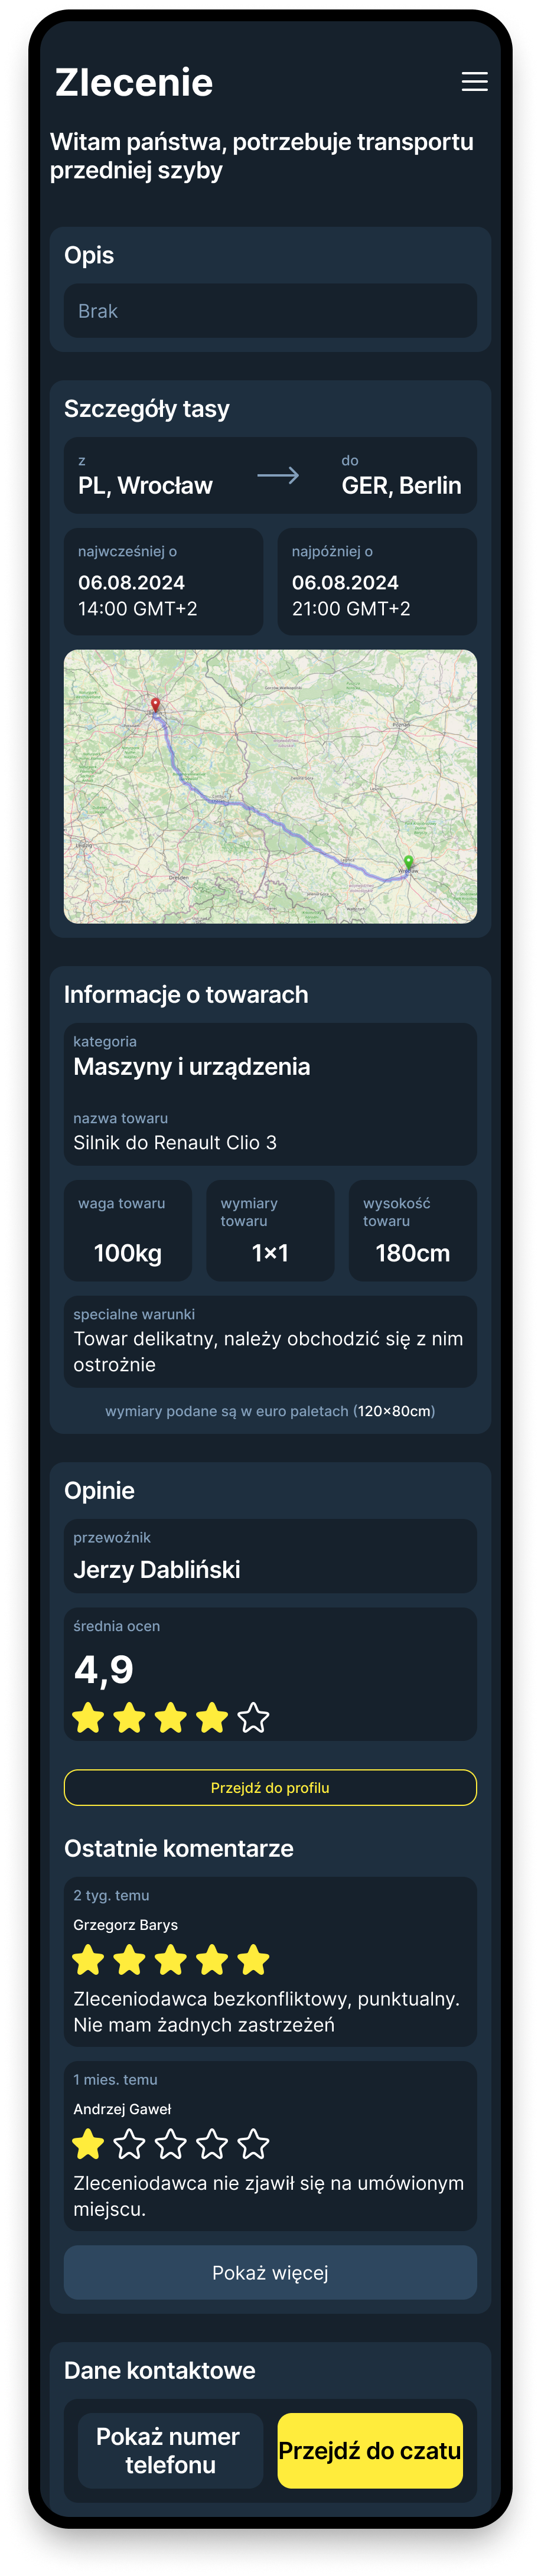
\includegraphics[width=0.25\linewidth]{rozdzial1/ogloszenie_zlecenie_m.png}}} &
    \vtop{\null\hbox{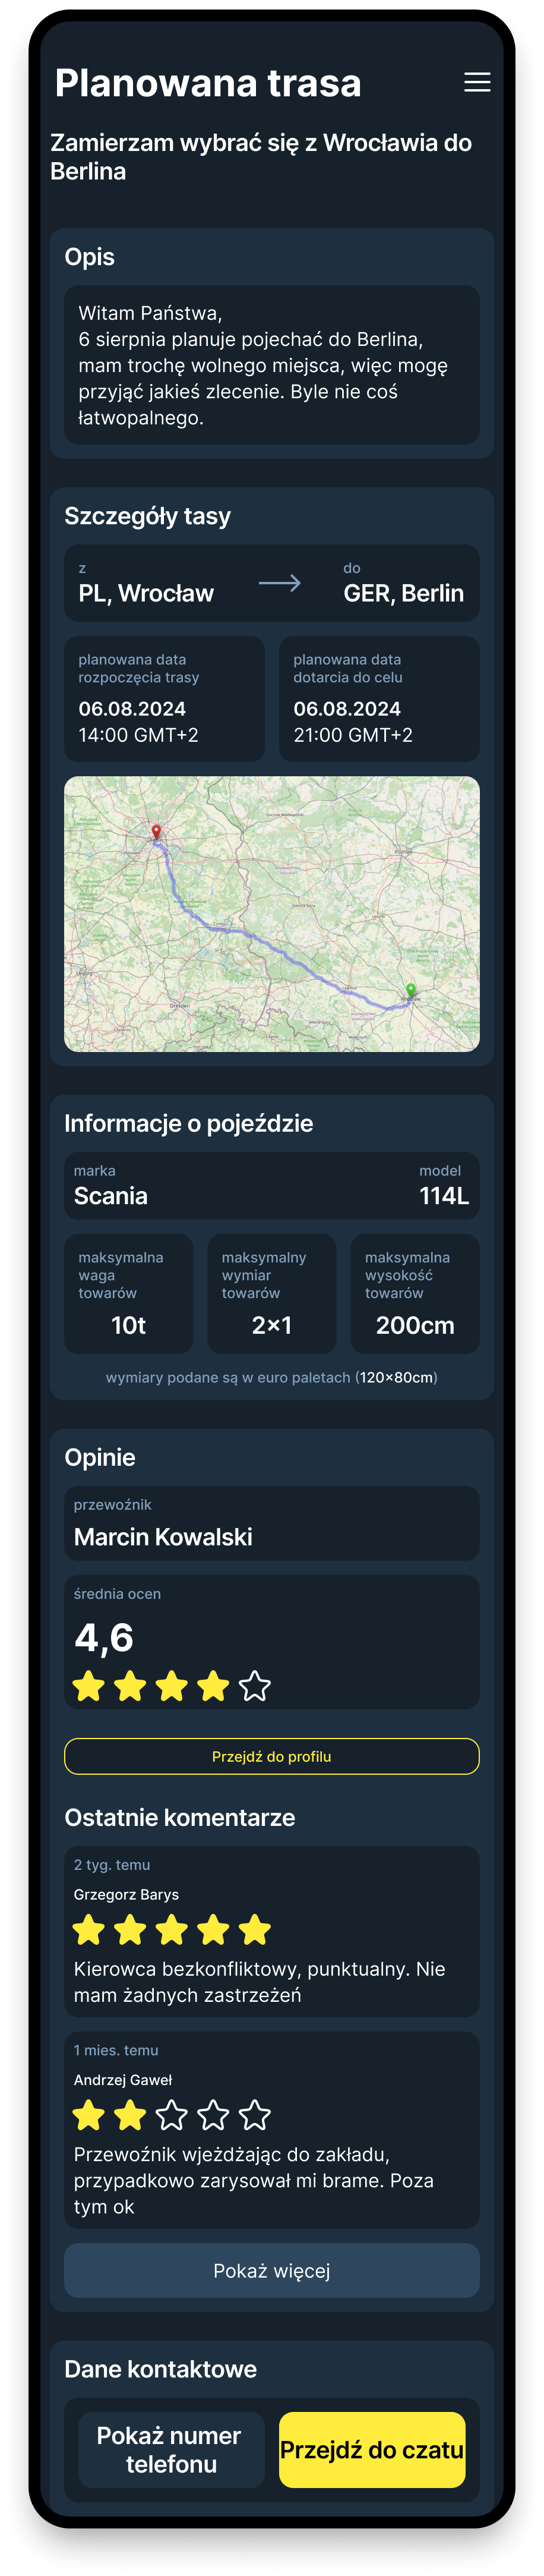
\includegraphics[width=0.25\linewidth]{rozdzial1/ogloszenie_planowana_trasa_m.png}}}
    \end{tabular}
    \caption{Wyświetlenie ogłoszenia w wersji mobilnej: a) Ogłoszenie zlecenia, b) Ogłoszenie o planowanej trasie}
	\label{Rys. fig:Wyświetlenie ogłoszenia - ab - mobile}
\end{figure}
\begin{figure}[H]
 \centering
  \begin{tabular}{@{}ccc@{}}
  a) & b)\\
  \vtop{\null\hbox{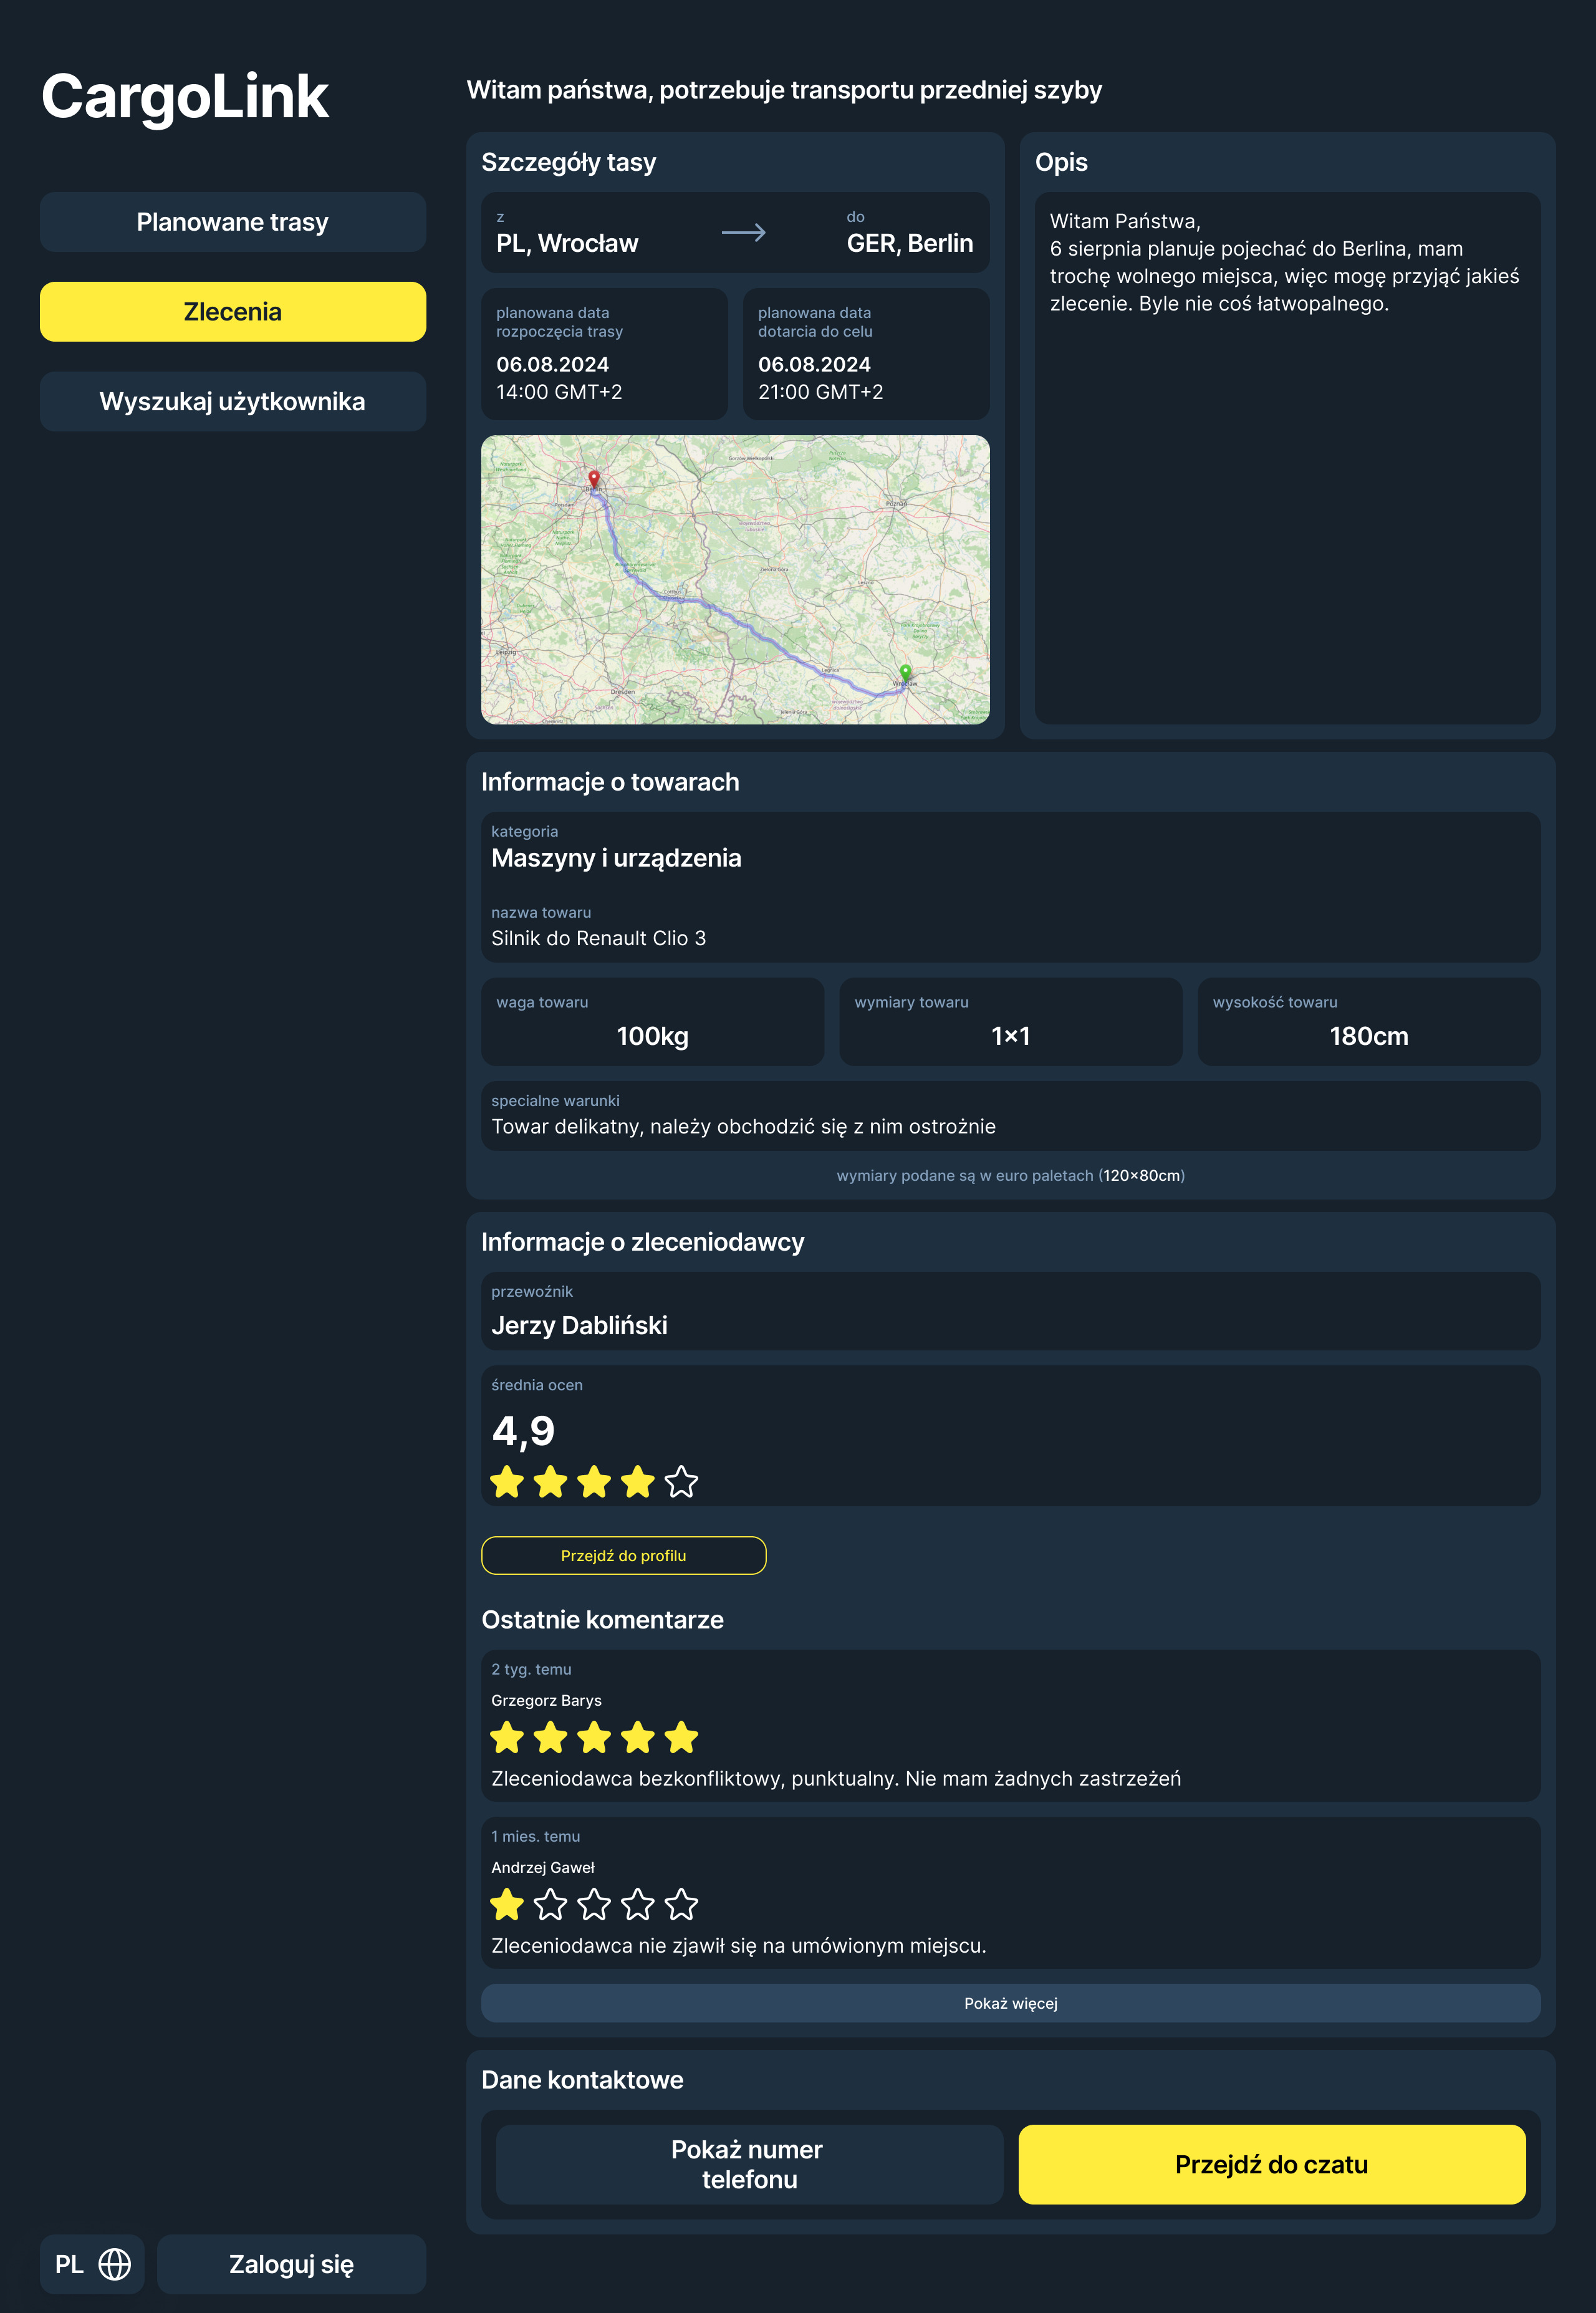
\includegraphics[width=0.45\textwidth]{rozdzial1/ogloszenie_zlecenie_d.jpg}}} &
  \vtop{\null\hbox{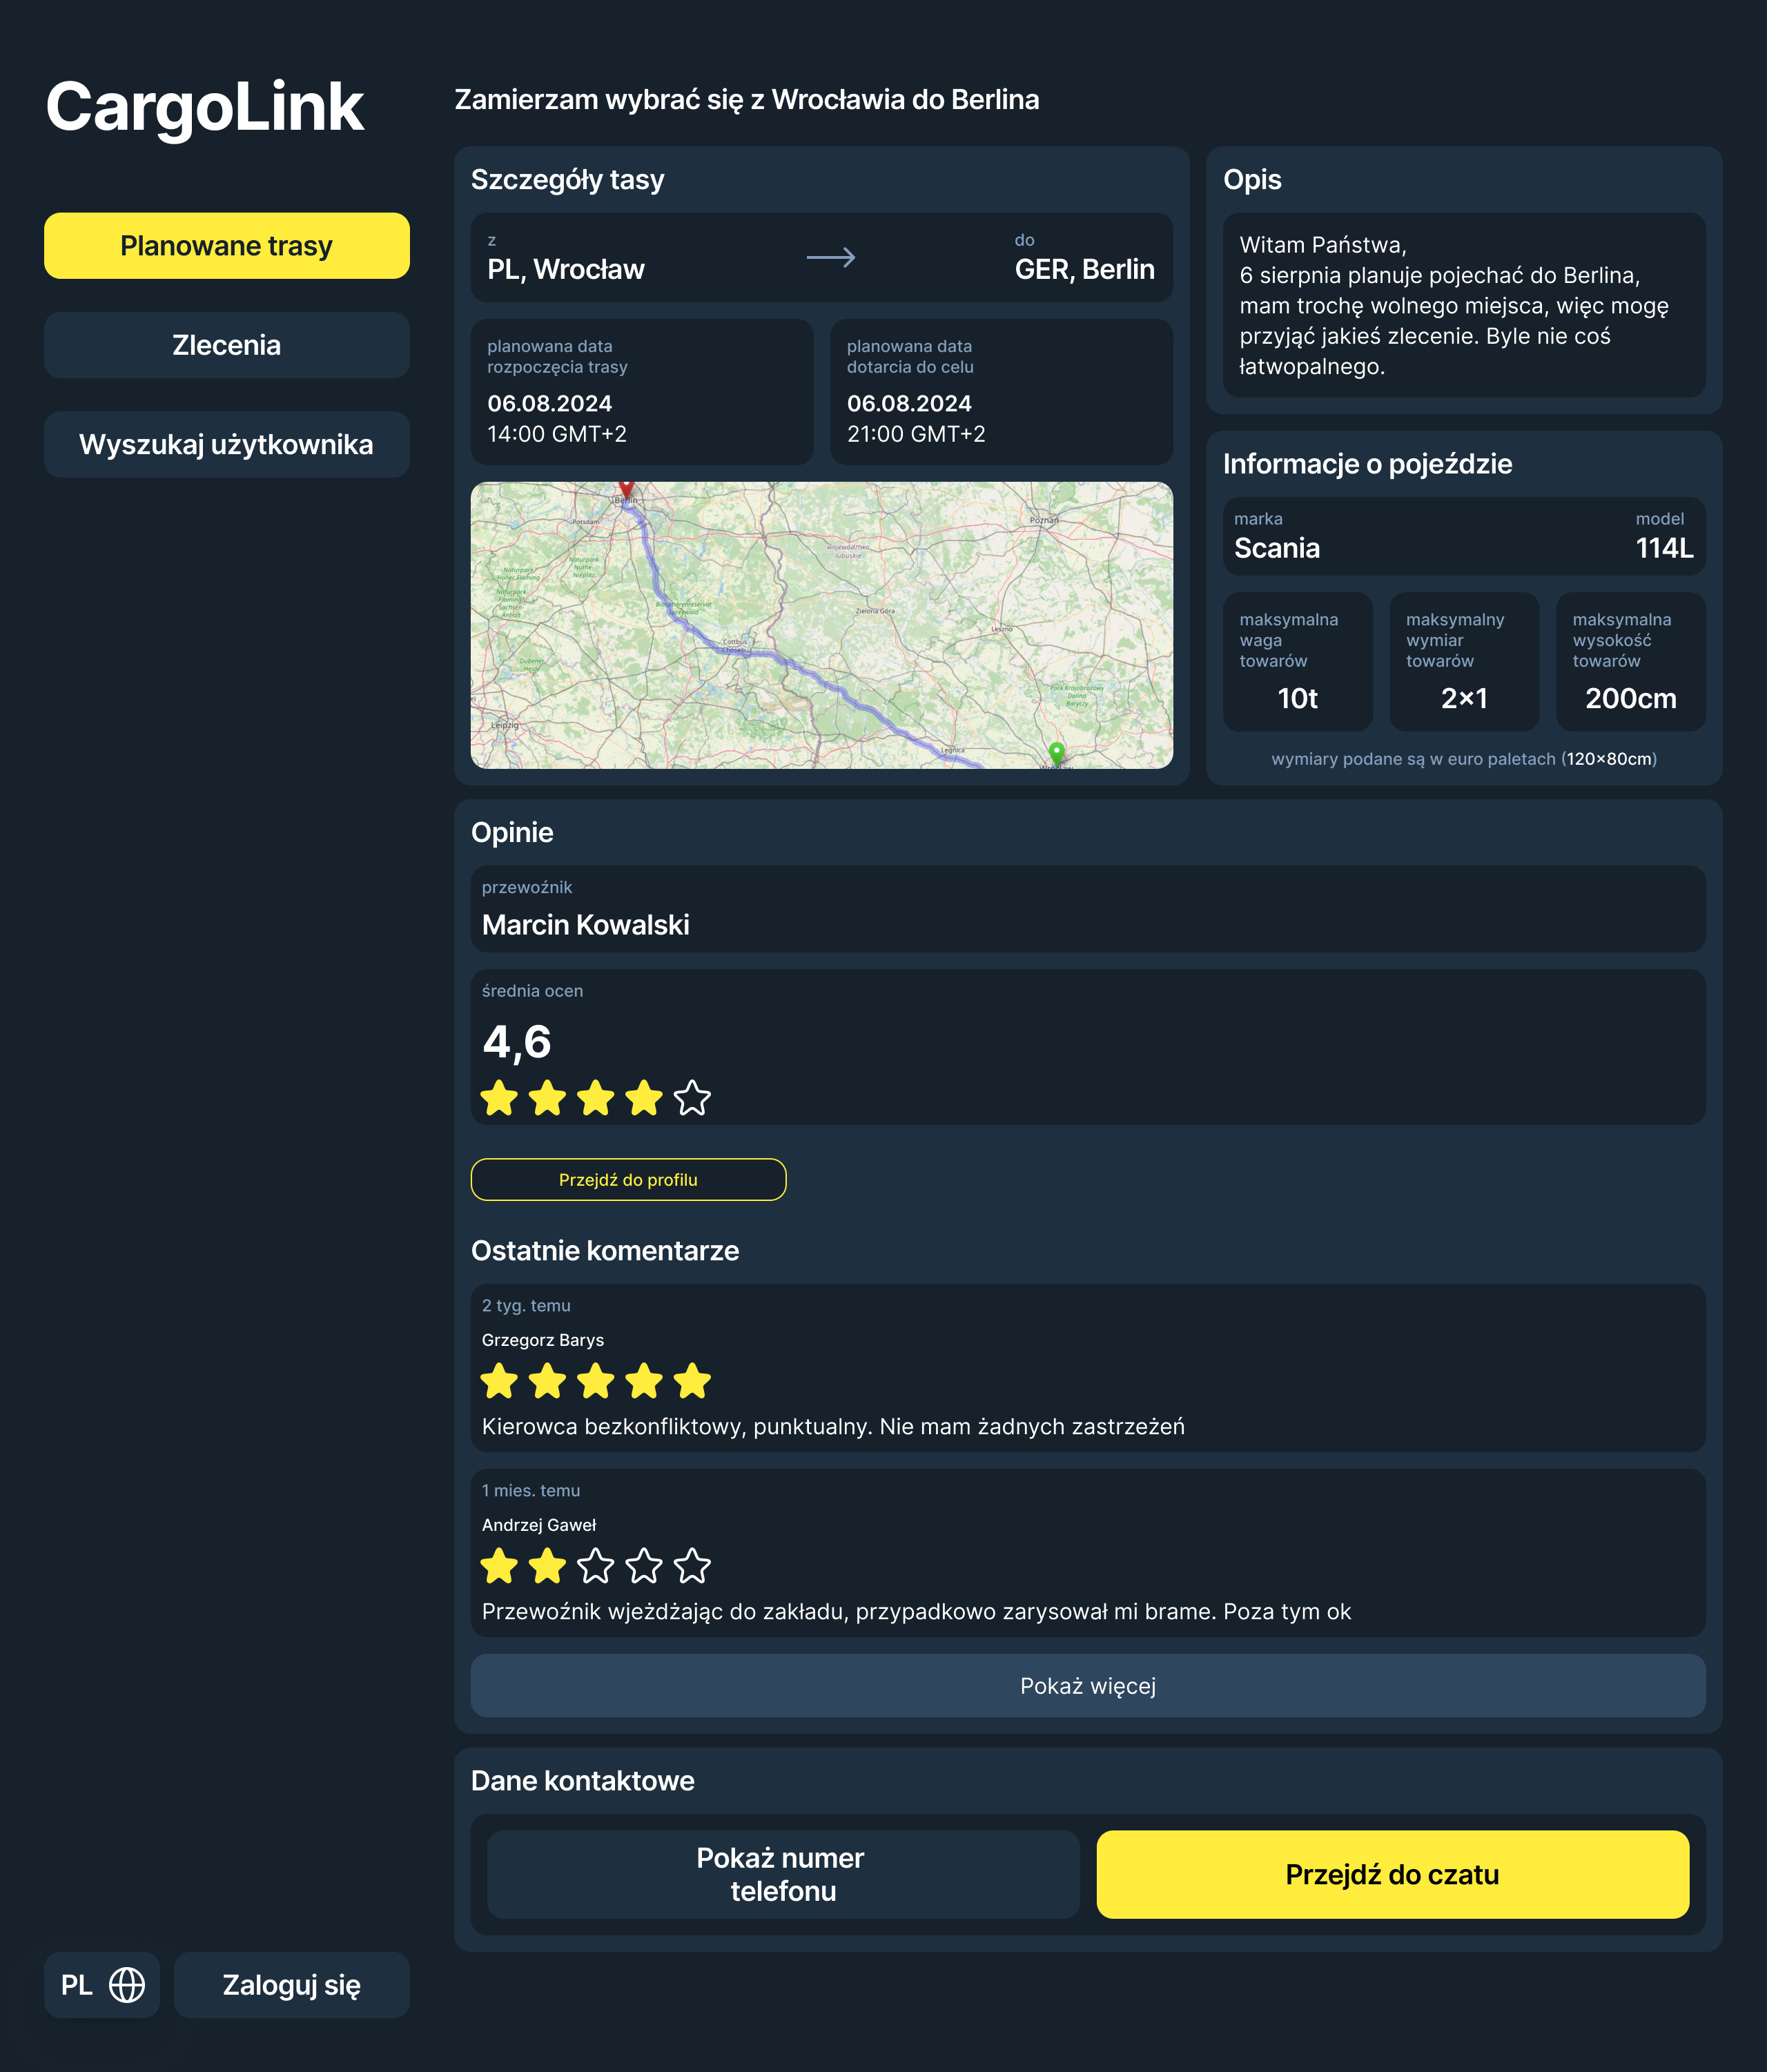
\includegraphics[width=0.45\textwidth]{rozdzial1/ogloszenie_planowana_trasa_d.jpg}}}
  \end{tabular}
 \caption{Wyświetlenie ogłoszenia w wersji desktopowej: a) Ogłoszenie zlecenia, b) Ogłoszenie o planowanej trasie}
 \label{Rys. fig:Wyświetlenie ogłoszenia - ab - desktop}
\end{figure}

\texttt{Wyświetlenie mapy ze wszystkimi trasami} \\
Zdarzenie inicjujące: Kliknięcie w przycisk \texttt{Otwórz mapę tras} (Rys. \ref{Rys. fig:Przeglądarka zleceń i planowanych tras - ab - mobile}.a lub \ref{Rys. fig:Przeglądarka zleceń i planowanych tras - ab - mobile}.b lub \ref{Rys. fig:Przeglądarka zleceń i planowanych tras - ab - desktop}.a lub \ref{Rys. fig:Przeglądarka zleceń i planowanych tras - ab - desktop}.b). \\
Warunki początkowe: Brak. \\
Przebieg podstawowy realizacji przypadku użycia:
\begin{enumerate}
    \item Wykonanie przypadku użycia \ref{Przeglądanie zleceń} lub \ref{Przeglądanie ogłoszeń planowanych tras};
    \item Kliknięcie w przycisk \texttt{Otwórz mapę tras} (Rys. \ref{Rys. fig:Przeglądarka zleceń i planowanych tras - ab - mobile}.a lub \ref{Rys. fig:Przeglądarka zleceń i planowanych tras - ab - mobile}.b lub \ref{Rys. fig:Przeglądarka zleceń i planowanych tras - ab - desktop}.a lub \ref{Rys. fig:Przeglądarka zleceń i planowanych tras - ab - desktop}.b);
    \item Wyświetlenie mapy z zaznaczonymi wszystkimi trasami w bazie danych, które są aktualne.
\end{enumerate}
Warunki końcowe: Użytkownikowi ukazuję się mapa z zaznaczonymi trasami wszystkich aktualnych ogłoszeń w bazie danych (Rys. \ref{Rys. fig:Mapa ze wszystkimi trasami - mobile} lub \ref{Rys. fig:Mapa ze wszystkimi trasami - desktop}).\\
\begin{figure}[H]
	\centering
		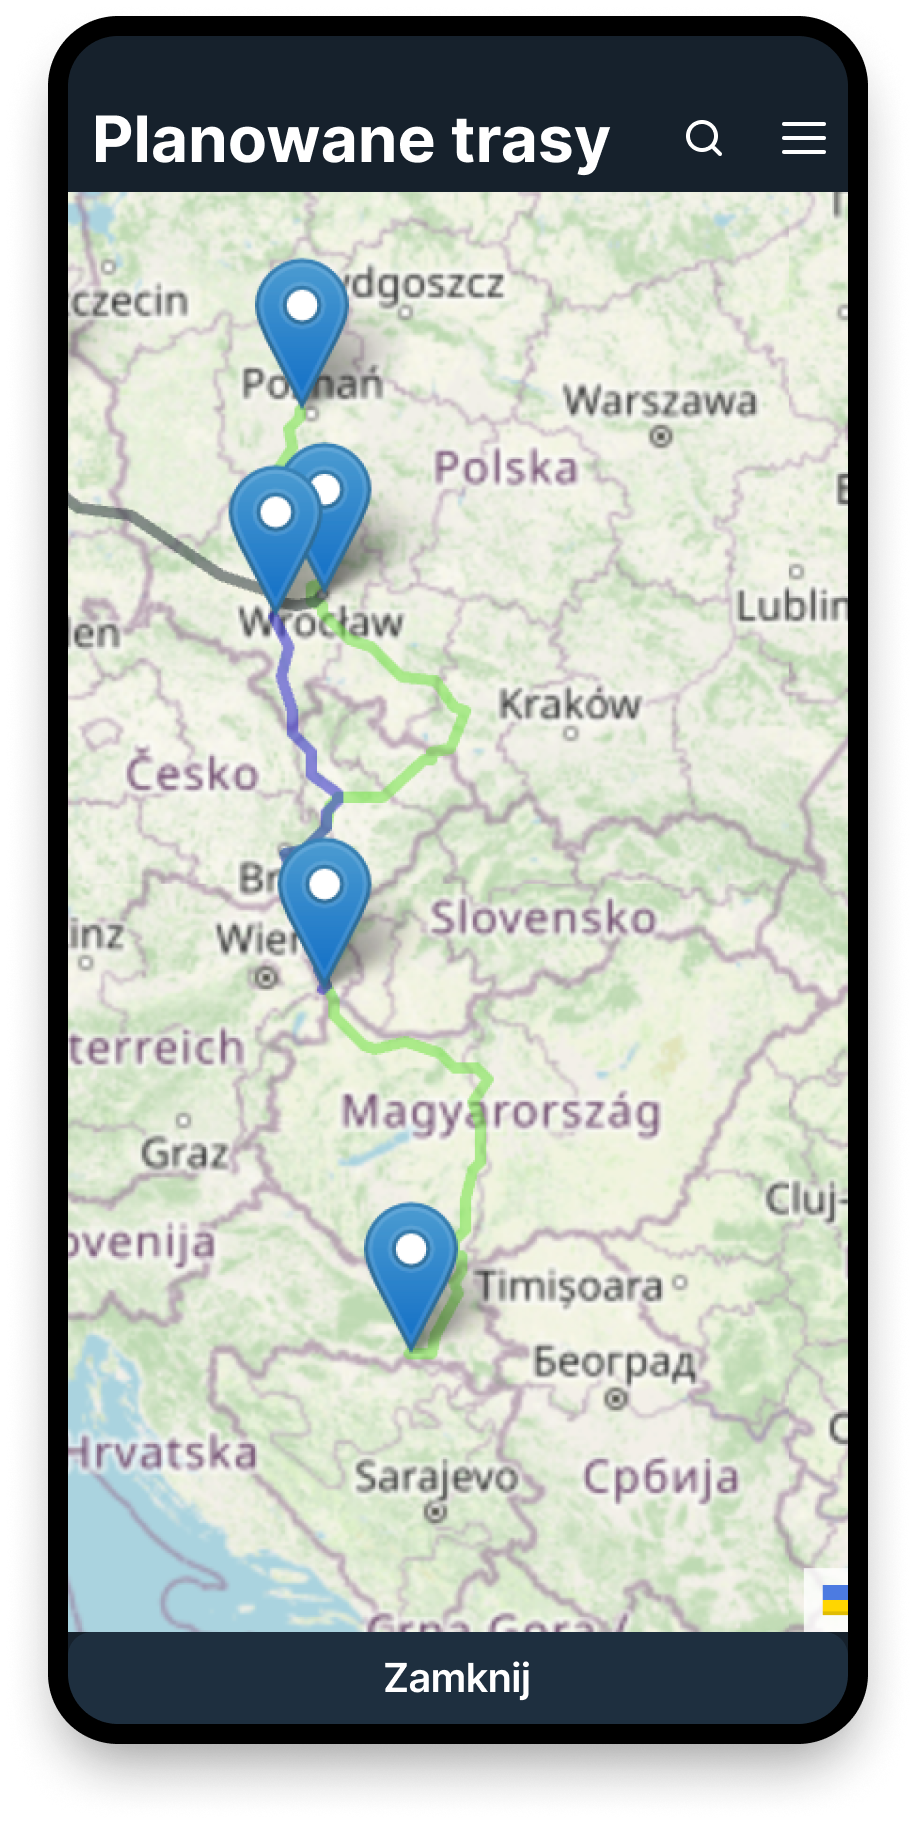
\includegraphics[width=0.3\linewidth]{rozdzial1/mapa_m.png}
	\caption{Mapa ze wszystkimi trasami w wersji mobilnej}
	\label{Rys. fig:Mapa ze wszystkimi trasami - mobile}
\end{figure}
\begin{figure}[H]
	\centering
		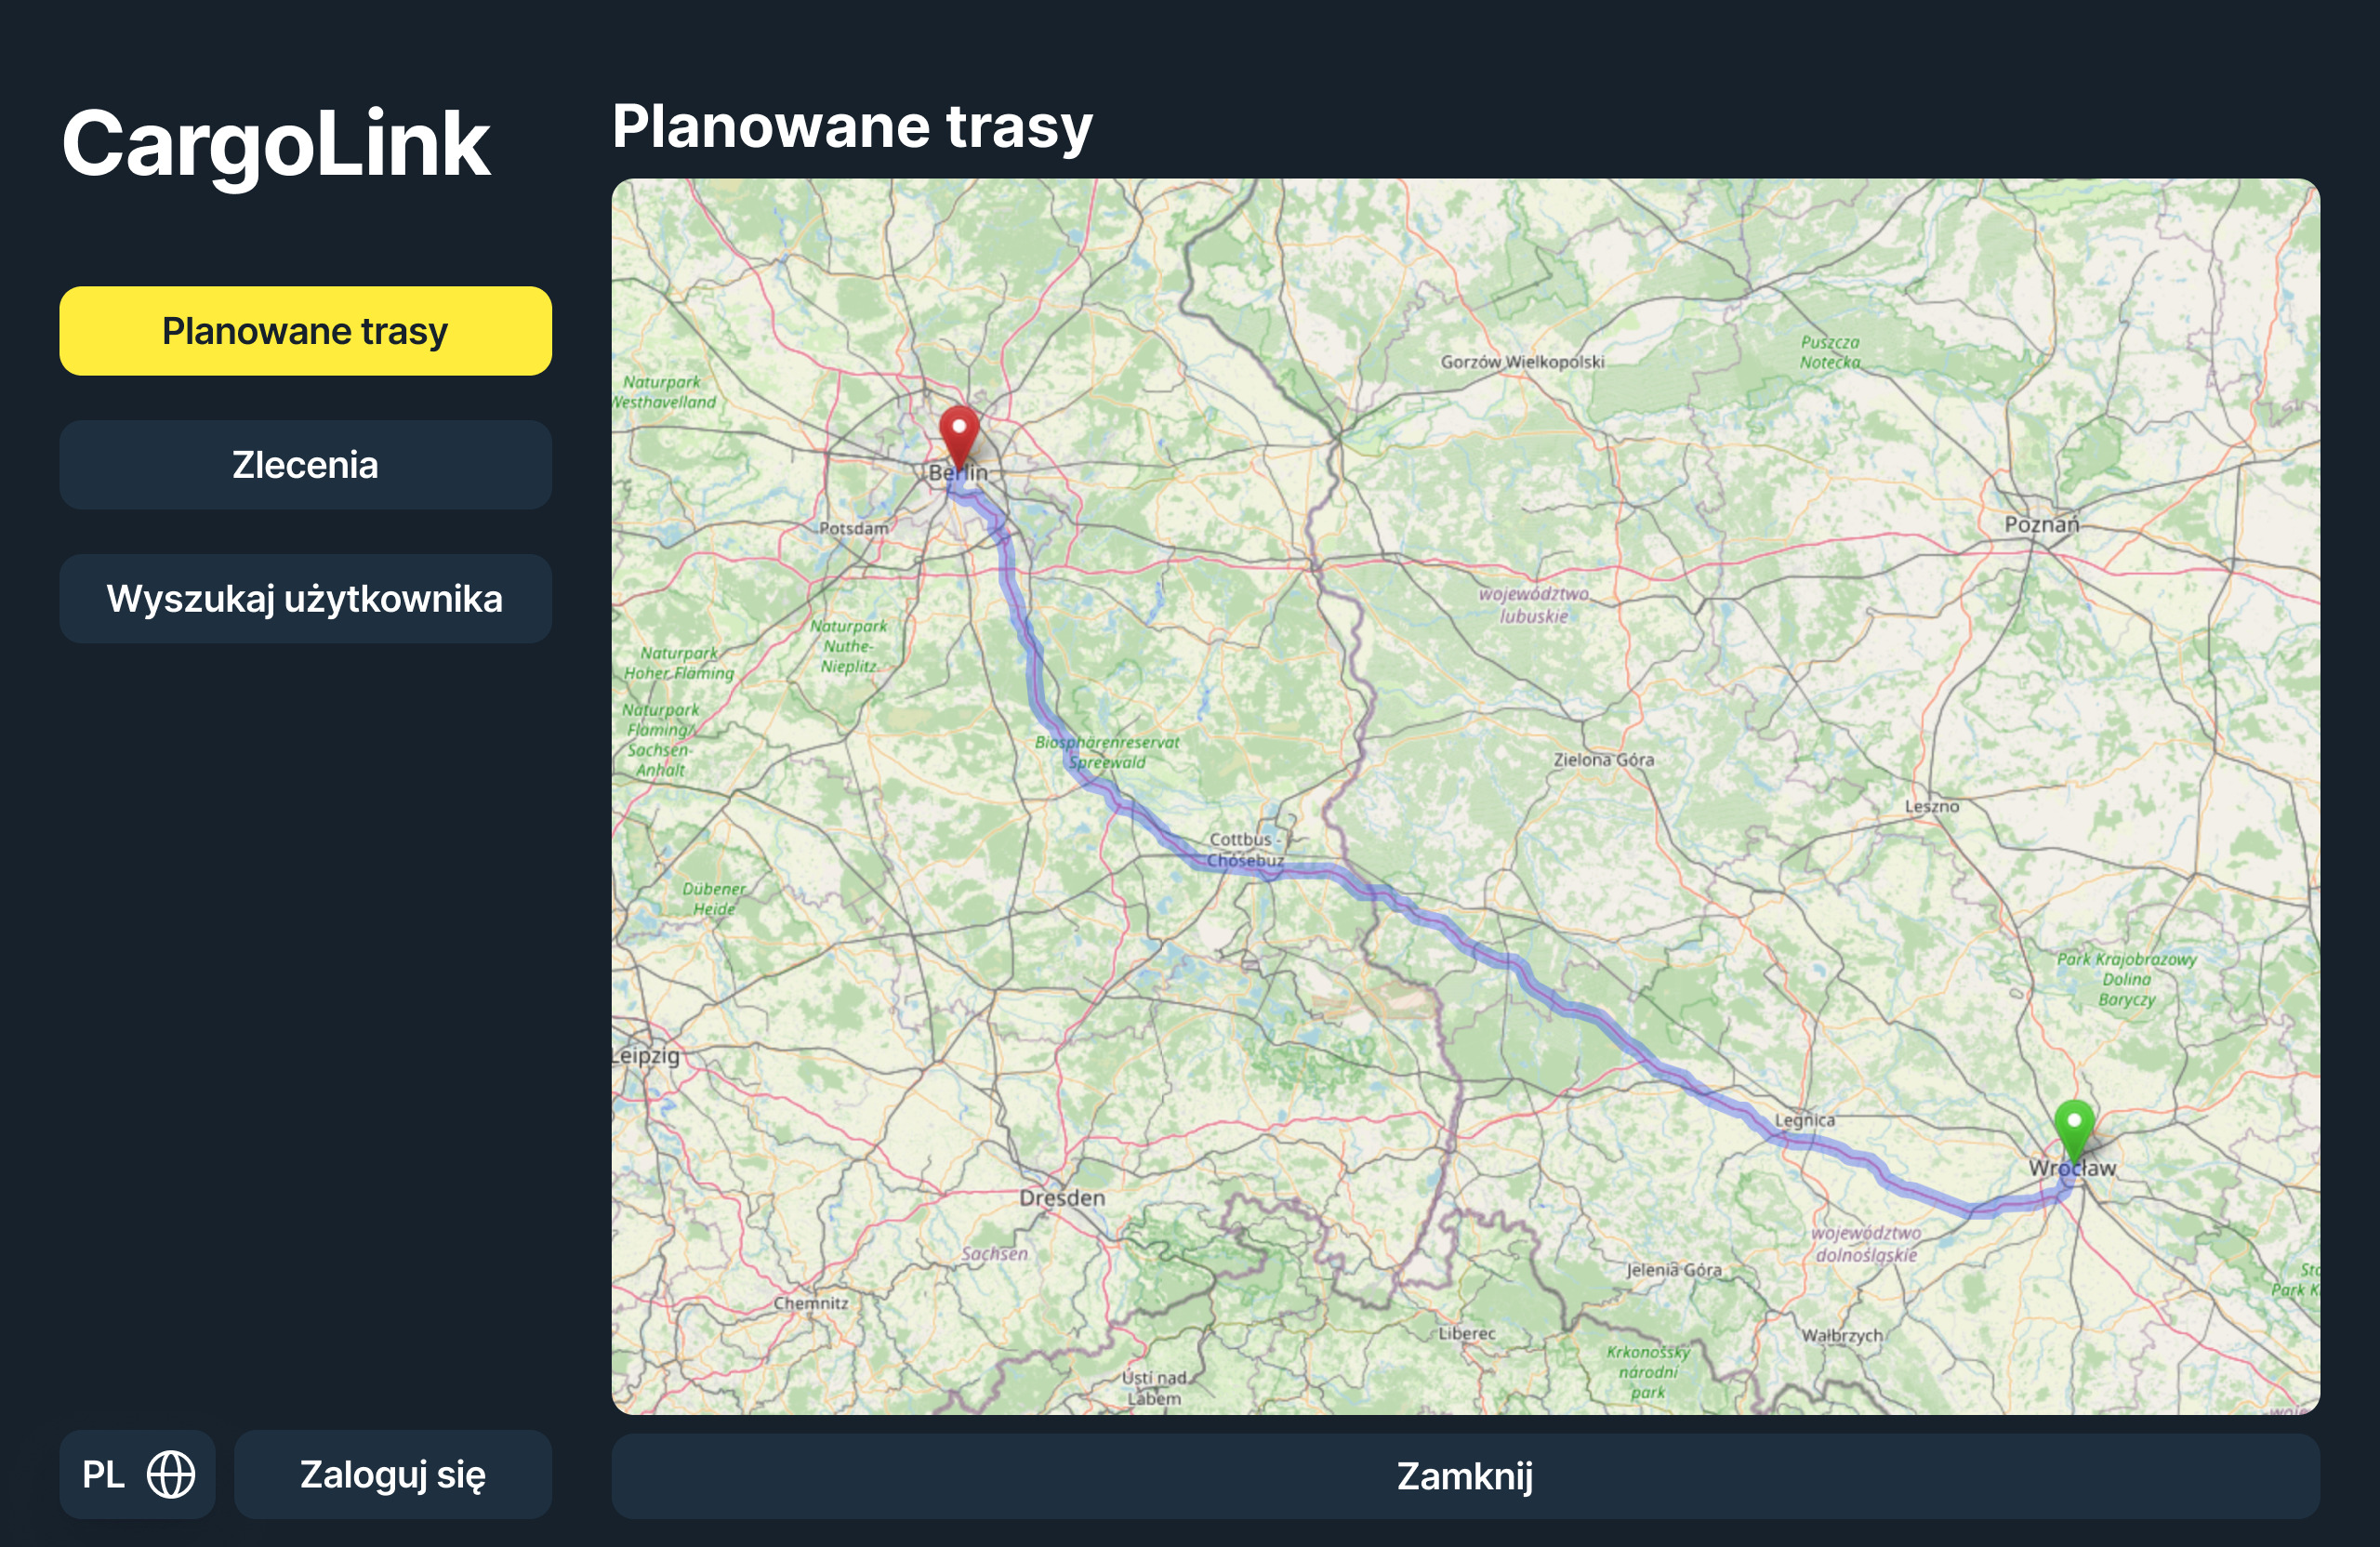
\includegraphics[width=0.7\linewidth]{rozdzial1/mapa_d.jpg}
	\caption{Mapa ze wszystkimi trasami w wersji desktopowej}
	\label{Rys. fig:Mapa ze wszystkimi trasami - desktop}
\end{figure}

\texttt{Wyświetlenie profilu użytkownika} \\
\label{Wyświetlenie profilu użytkownika}
Zdarzenie inicjujące: Kliknięcie w dowolnego użytkownika (Rys. \ref{Rys. fig:Przeglądarka zleceń i planowanych tras - ab - mobile}.a lub \ref{Rys. fig:Przeglądarka zleceń i planowanych tras - ab - mobile}.b) lub kliknięcie w imię i nazwisko autora dowolnego ogłoszenia (Rys. \ref{Rys. fig:Wyświetlenie ogłoszenia - ab - mobile}.a lub \ref{Rys. fig:Wyświetlenie ogłoszenia - ab - mobile}.b lub \ref{Rys. fig:Wyświetlenie ogłoszenia - ab - desktop}.a lub \ref{Rys. fig:Wyświetlenie ogłoszenia - ab - desktop}.b) \\
Warunki początkowe: Brak. \\
Przebieg podstawowy realizacji przypadku użycia:
\begin{enumerate}
    \item Kliknięcie w dowolnego użytkownika (Rys. \ref{Rys. fig:Przeglądarka zleceń i planowanych tras - ab - mobile}.a lub \ref{Rys. fig:Przeglądarka zleceń i planowanych tras - ab - mobile}.b) lub kliknięcie w imię i nazwisko autora dowolnego ogłoszenia (Rys. \ref{Rys. fig:Wyświetlenie ogłoszenia - ab - mobile}.a lub \ref{Rys. fig:Wyświetlenie ogłoszenia - ab - mobile}.b lub \ref{Rys. fig:Wyświetlenie ogłoszenia - ab - desktop}.a lub \ref{Rys. fig:Wyświetlenie ogłoszenia - ab - desktop}.b);
    \item Wyświetlenie profilu wybranego użytkownika (Rys. \ref{Rys. fig:Profil użytkownika - mobile} lub \ref{Rys. fig:Profil użytkownika - desktop}).
\end{enumerate}
Warunki końcowe: Użytkownik przechodzi do strony profilu wybranego użytkownika (Rys. \ref{Rys. fig:Profil użytkownika - mobile} lub \ref{Rys. fig:Profil użytkownika - desktop}).
\begin{figure}[H]
	\centering
		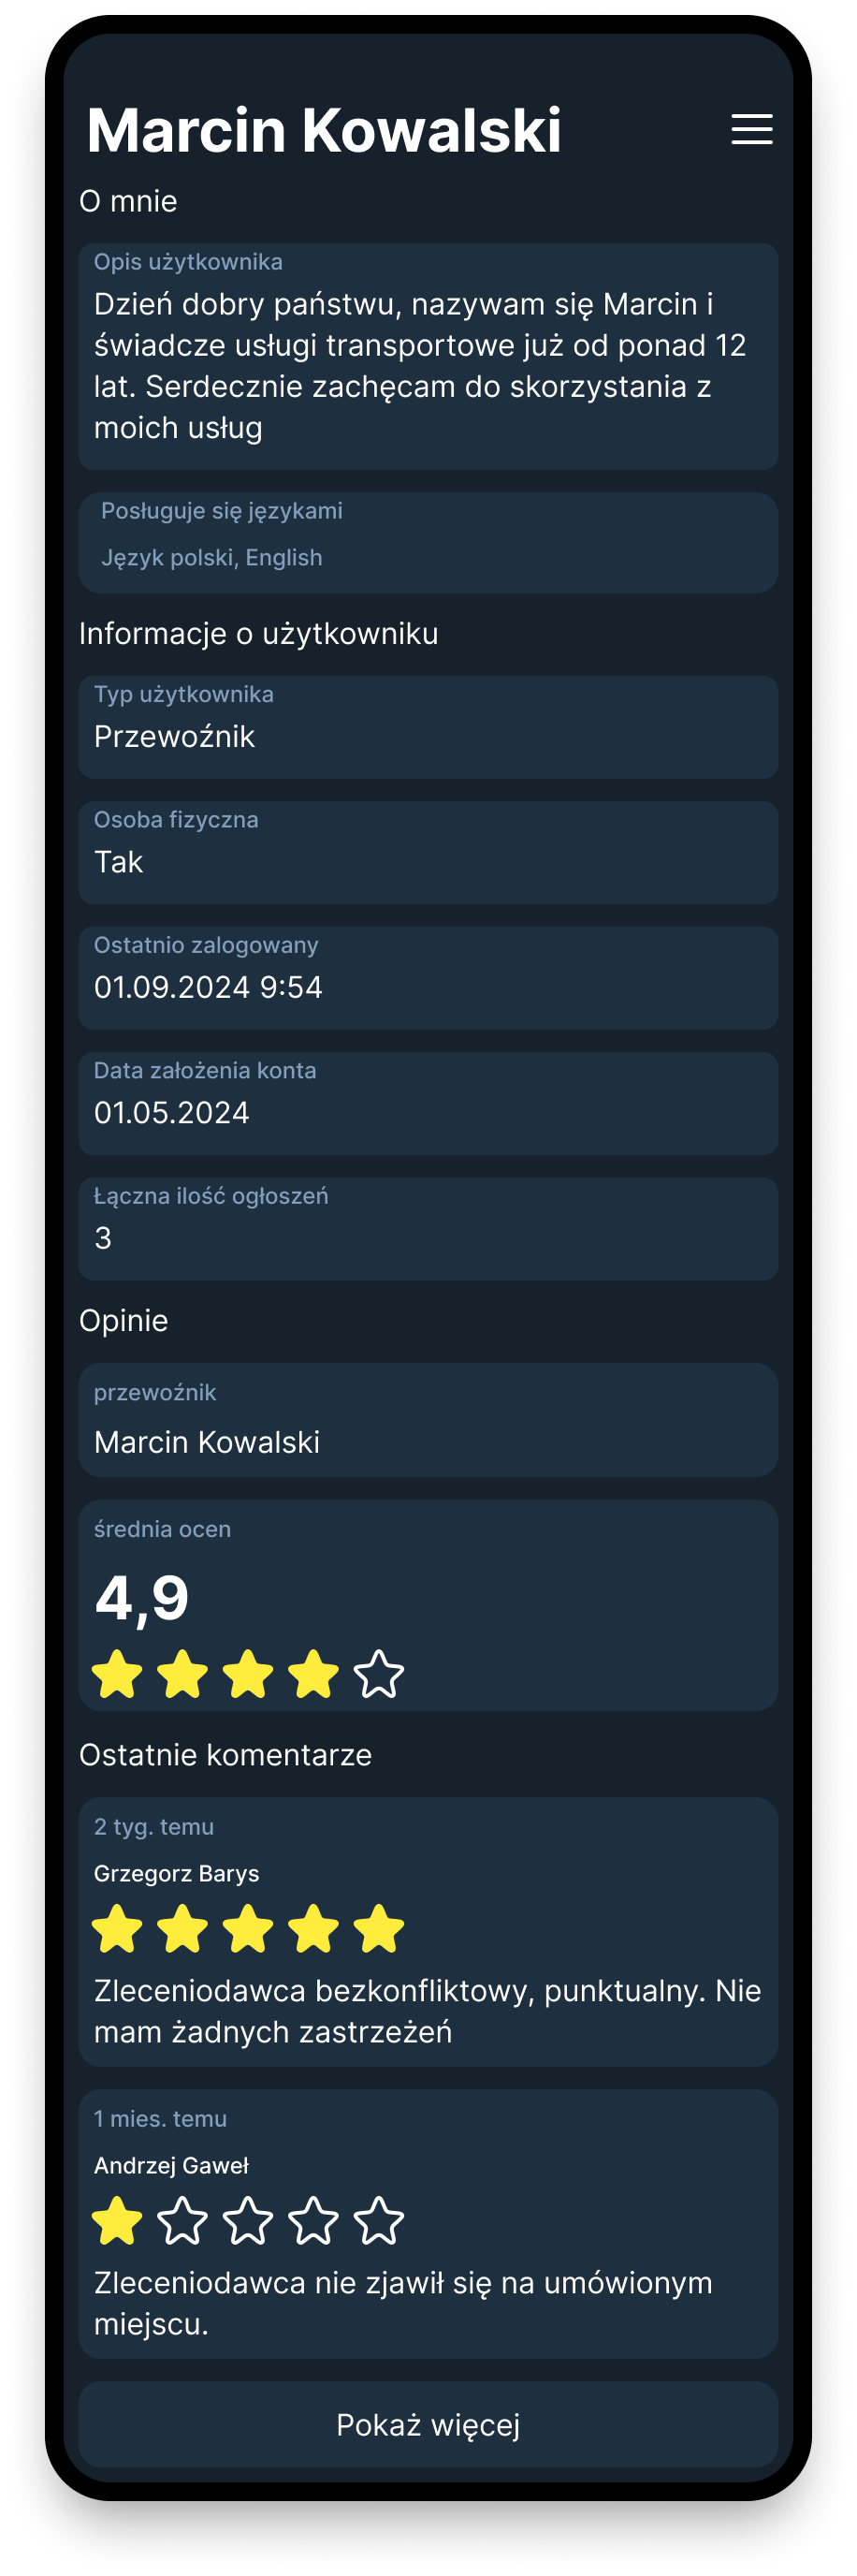
\includegraphics[width=0.3\linewidth]{rozdzial1/profil_m.png}
	\caption{Profil użytkownika w wersji mobilnej}
	\label{Rys. fig:Profil użytkownika - mobile}
\end{figure}
\begin{figure}[H]
	\centering
		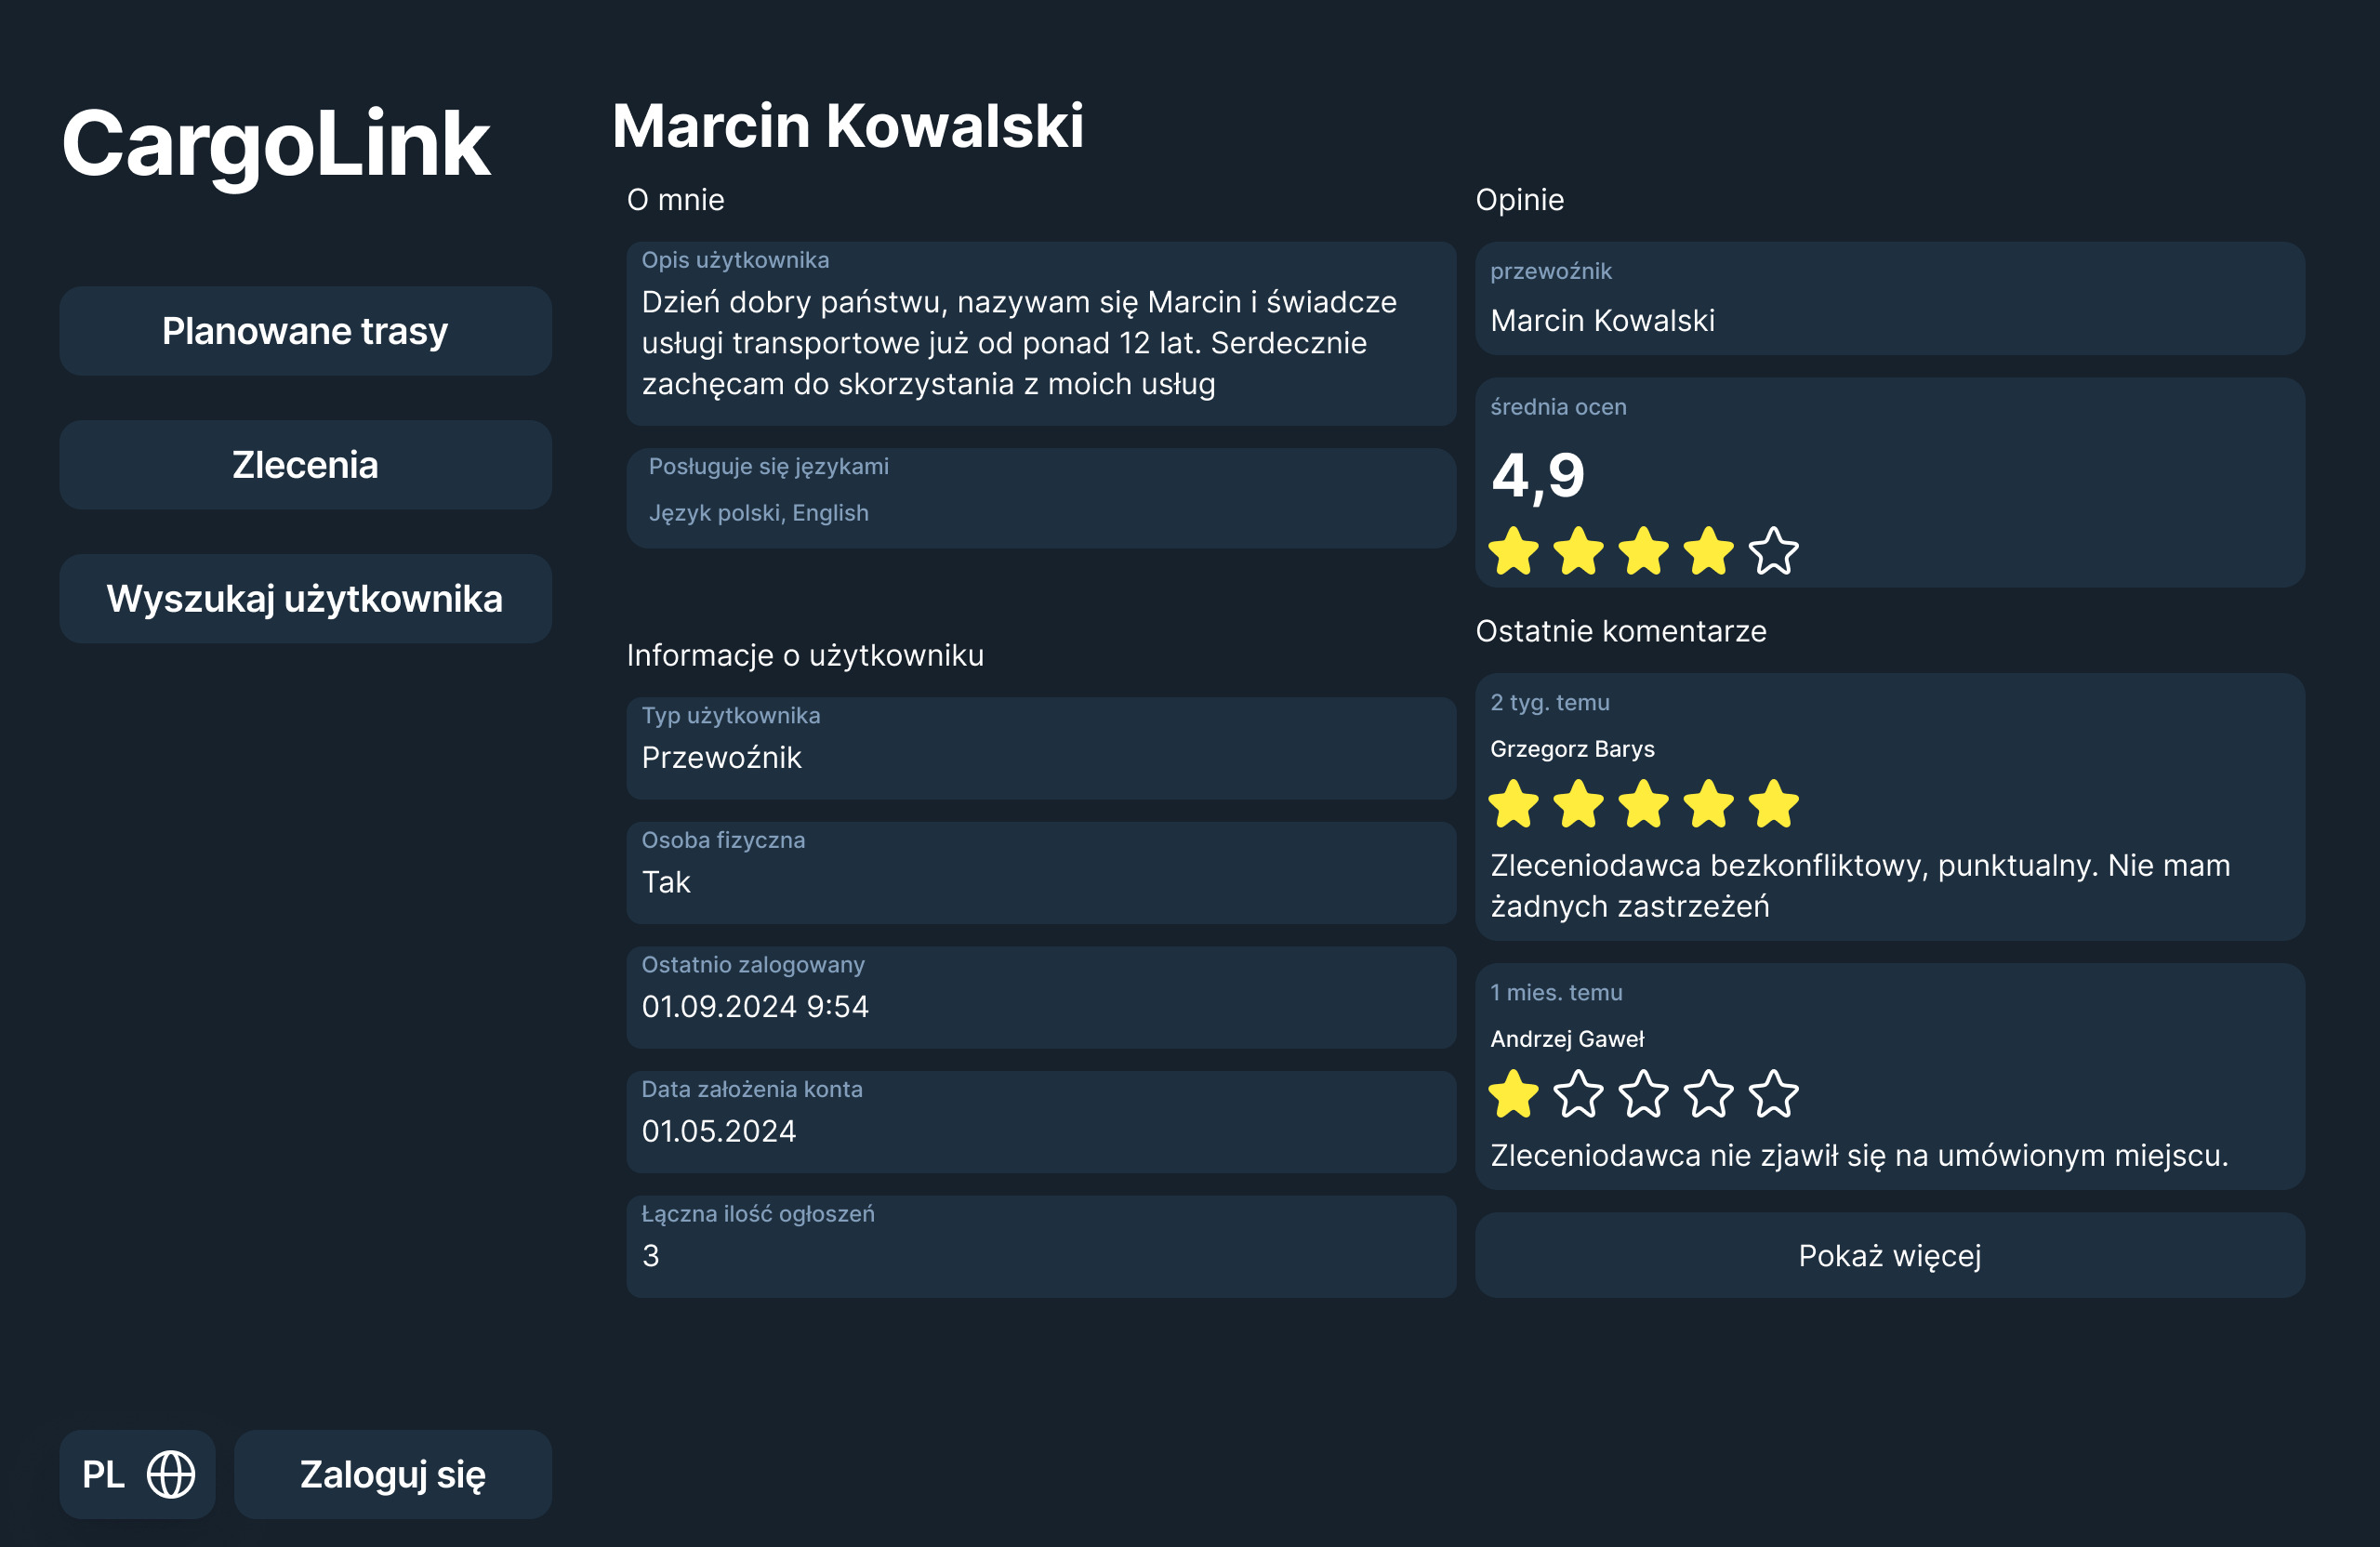
\includegraphics[width=0.7\linewidth]{rozdzial1/profil_d.jpg}
	\caption{Profil użytkownika w wersji desktopowej}
	\label{Rys. fig:Profil użytkownika - desktop}
\end{figure}

\subsection{Przewoźnik}
\begin{figure}[H]
	\centering
		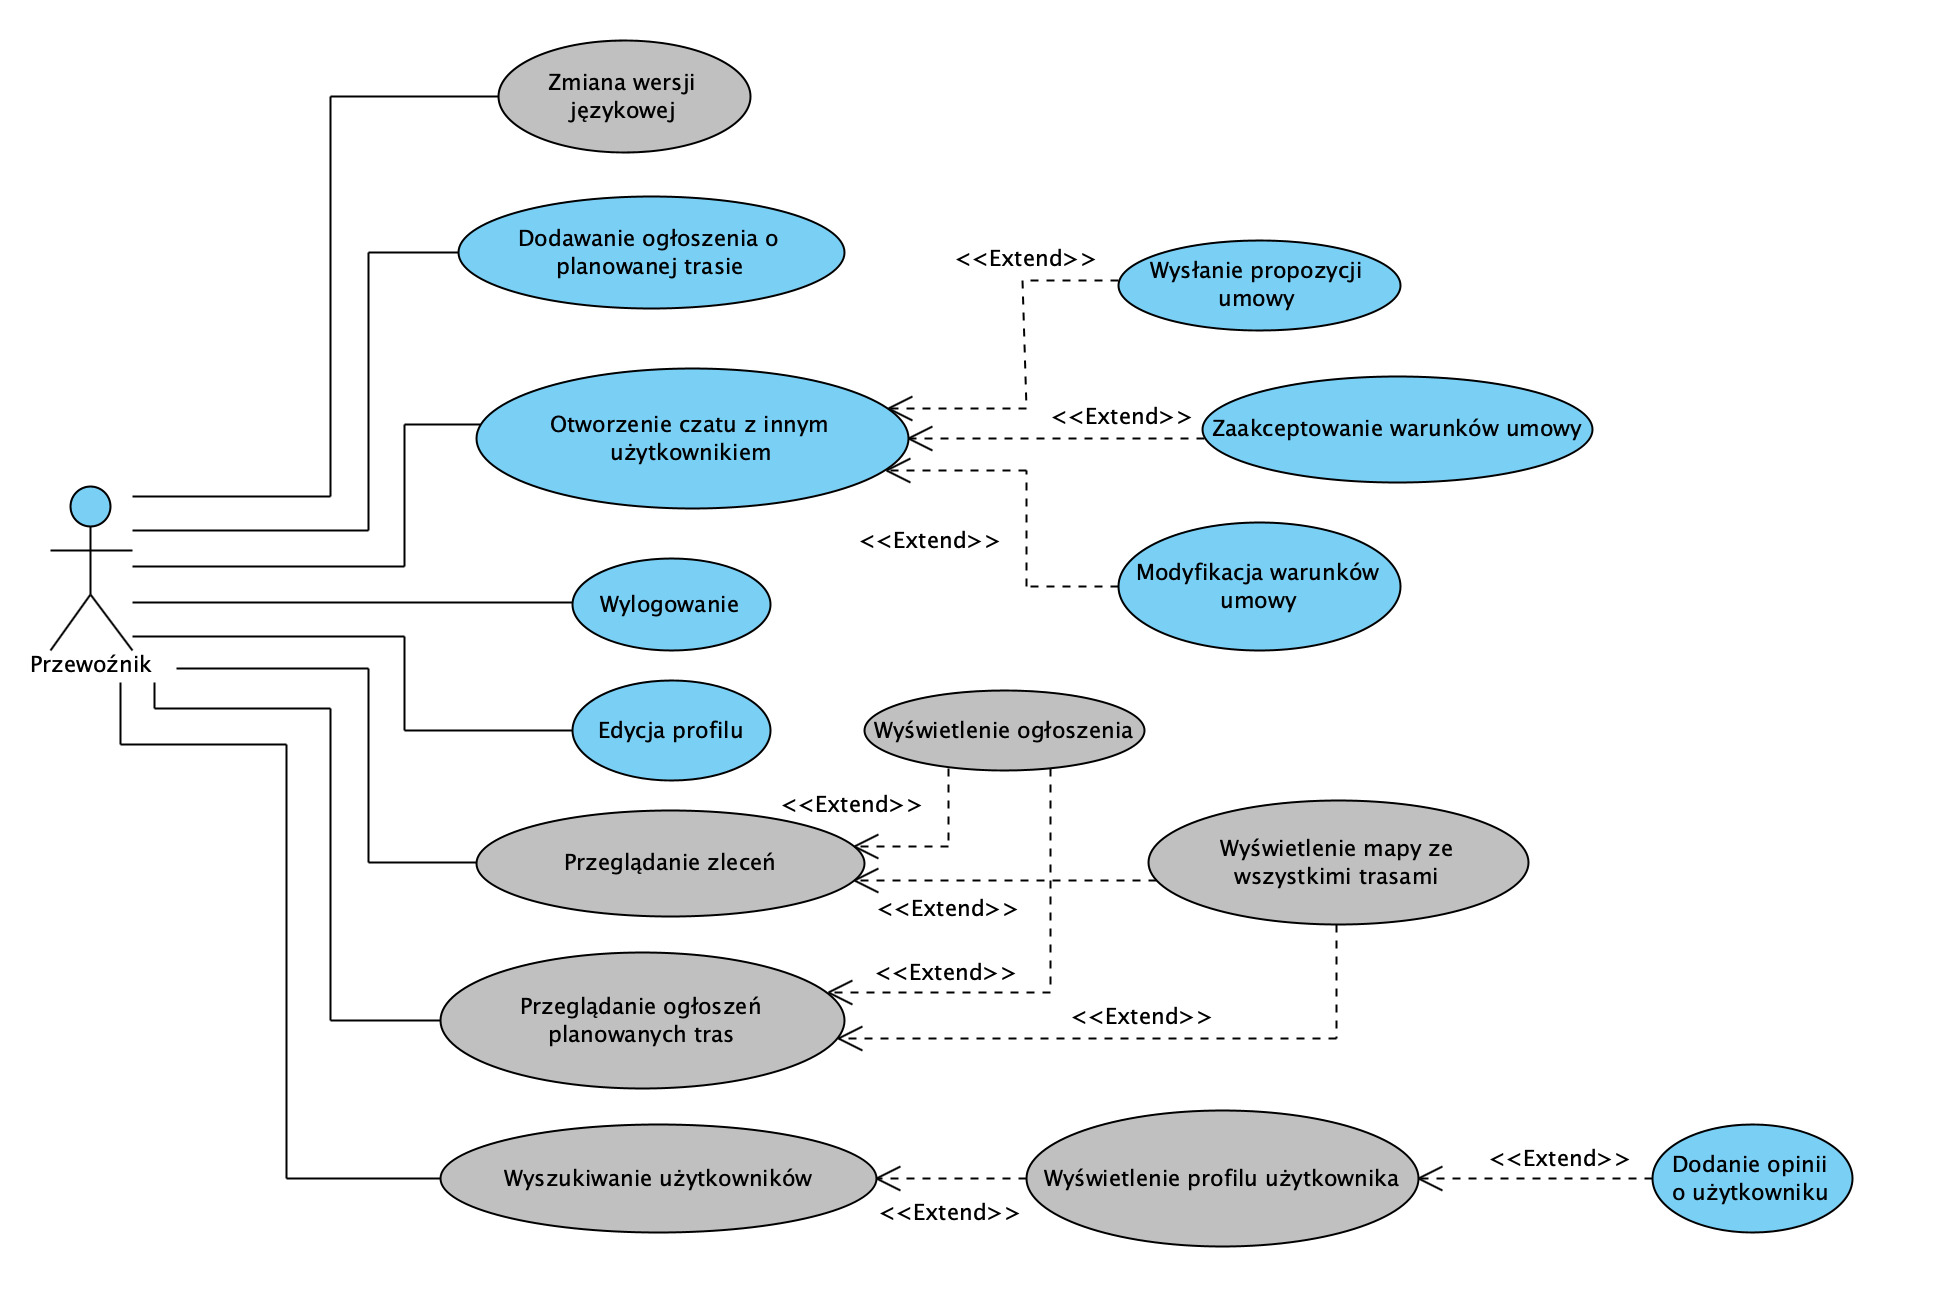
\includegraphics[width=\linewidth]{rozdzial1/PU_przewoznik.jpg}
	\caption{Diagram przedstawiający przypadki użycia aktora \texttt{Przewoźnik}}
	\label{Rys. fig:Diagram przedstawiający przypadki użycia aktora Przewoźnik}
\end{figure}
Na powyższym diagramie przedstawione zostały przypadki użycia dla \texttt{Przewoźnika}. Kolorem szarym oznaczone zostały przypadki użycia, które zostały już opisane w poprzednich podsekcjach.\\

\pagebreak
\texttt{Dodawanie nowego ogłoszenia o planowanej trasie} \\
Zdarzenie inicjujące: Po zalogowaniu na konto z typem przewoźnik, do menu nawigacji dokładane jest kilka nowych opcji. Kliknięcie w przycisk \texttt{Dodaj ogłoszenie o planowanej trasie} (Rys. \ref{Rys. fig:Dodawanie nowego ogłoszenia o planowanej trasie - ab - mobile}.a lub \ref{Rys. fig:Dodawanie nowego ogłoszenia o planowanej trasie - ab - desktop}.a). \\
Warunki początkowe: Bycie zalogowanym jako przewoźnik. \\
Przebieg podstawowy realizacji przypadku użycia:
\begin{enumerate}
    \item Kliknięcie w przycisk \texttt{Dodaj ogłoszenie o planowanej trasie} (Rys. \ref{Rys. fig:Dodawanie nowego ogłoszenia o planowanej trasie - ab - mobile}.a lub \ref{Rys. fig:Dodawanie nowego ogłoszenia o planowanej trasie - ab - desktop}.a);
    \item Wypełnienie formularza (Rys. \ref{Rys. fig:Dodawanie nowego ogłoszenia o planowanej trasie - ab - mobile}.b lub \ref{Rys. fig:Dodawanie nowego ogłoszenia o planowanej trasie - ab - desktop}.b;
    \item Kliknięcie przycisku \texttt{Dodaj ogłoszenie o planowanej trasie};
    \item System sprawdza poprawność wprowadzonych danych;
    \item Ogłoszenie wysyłane jest do akceptacji przez jednego z moderatorów.
\end{enumerate}
Warunki końcowe: Ogłoszenie o planowanej trasie wysyłane jest do moderatorów w celu akceptacji.
Przebieg alternatywny realizacji podpunktu (4a): Wprowadzone dane są niepoprawne. System informuje o niepowodzeniu. \\
\begin{figure}[H]
	\centering
	\begin{tabular}{@{}ccc@{}}
            a) & b)\\
    \vtop{\null\hbox{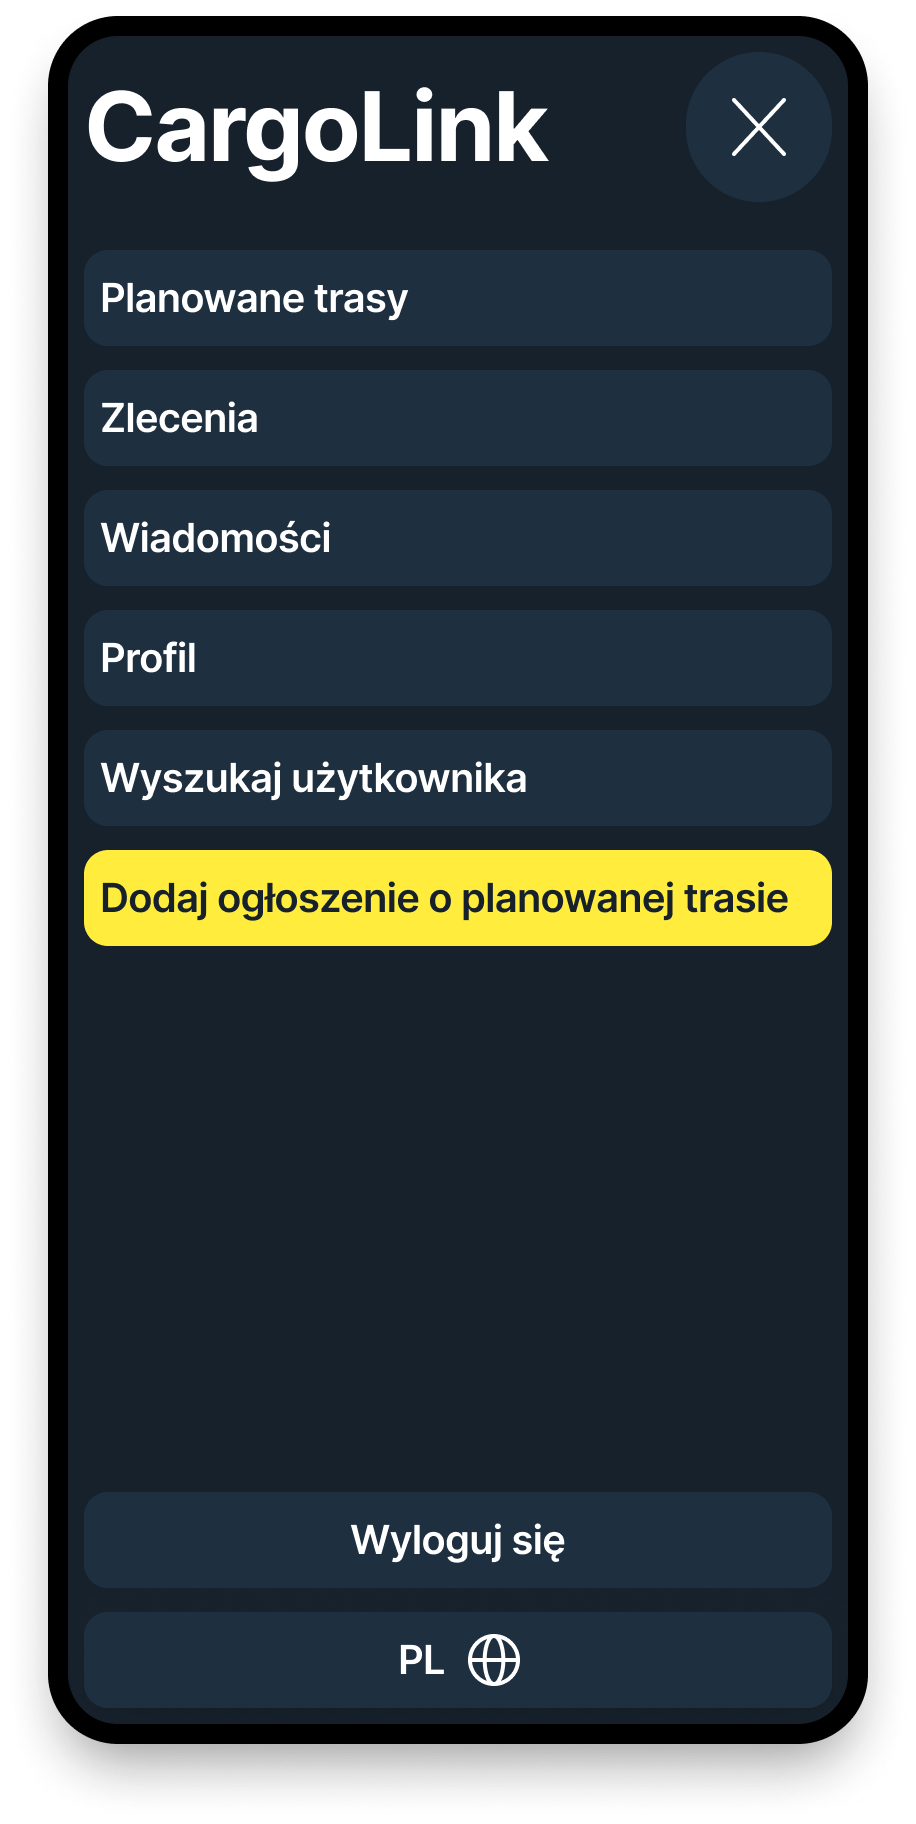
\includegraphics[width=0.3\linewidth]{rozdzial1/menu_m_przewoznik.png}}} &
    \vtop{\null\hbox{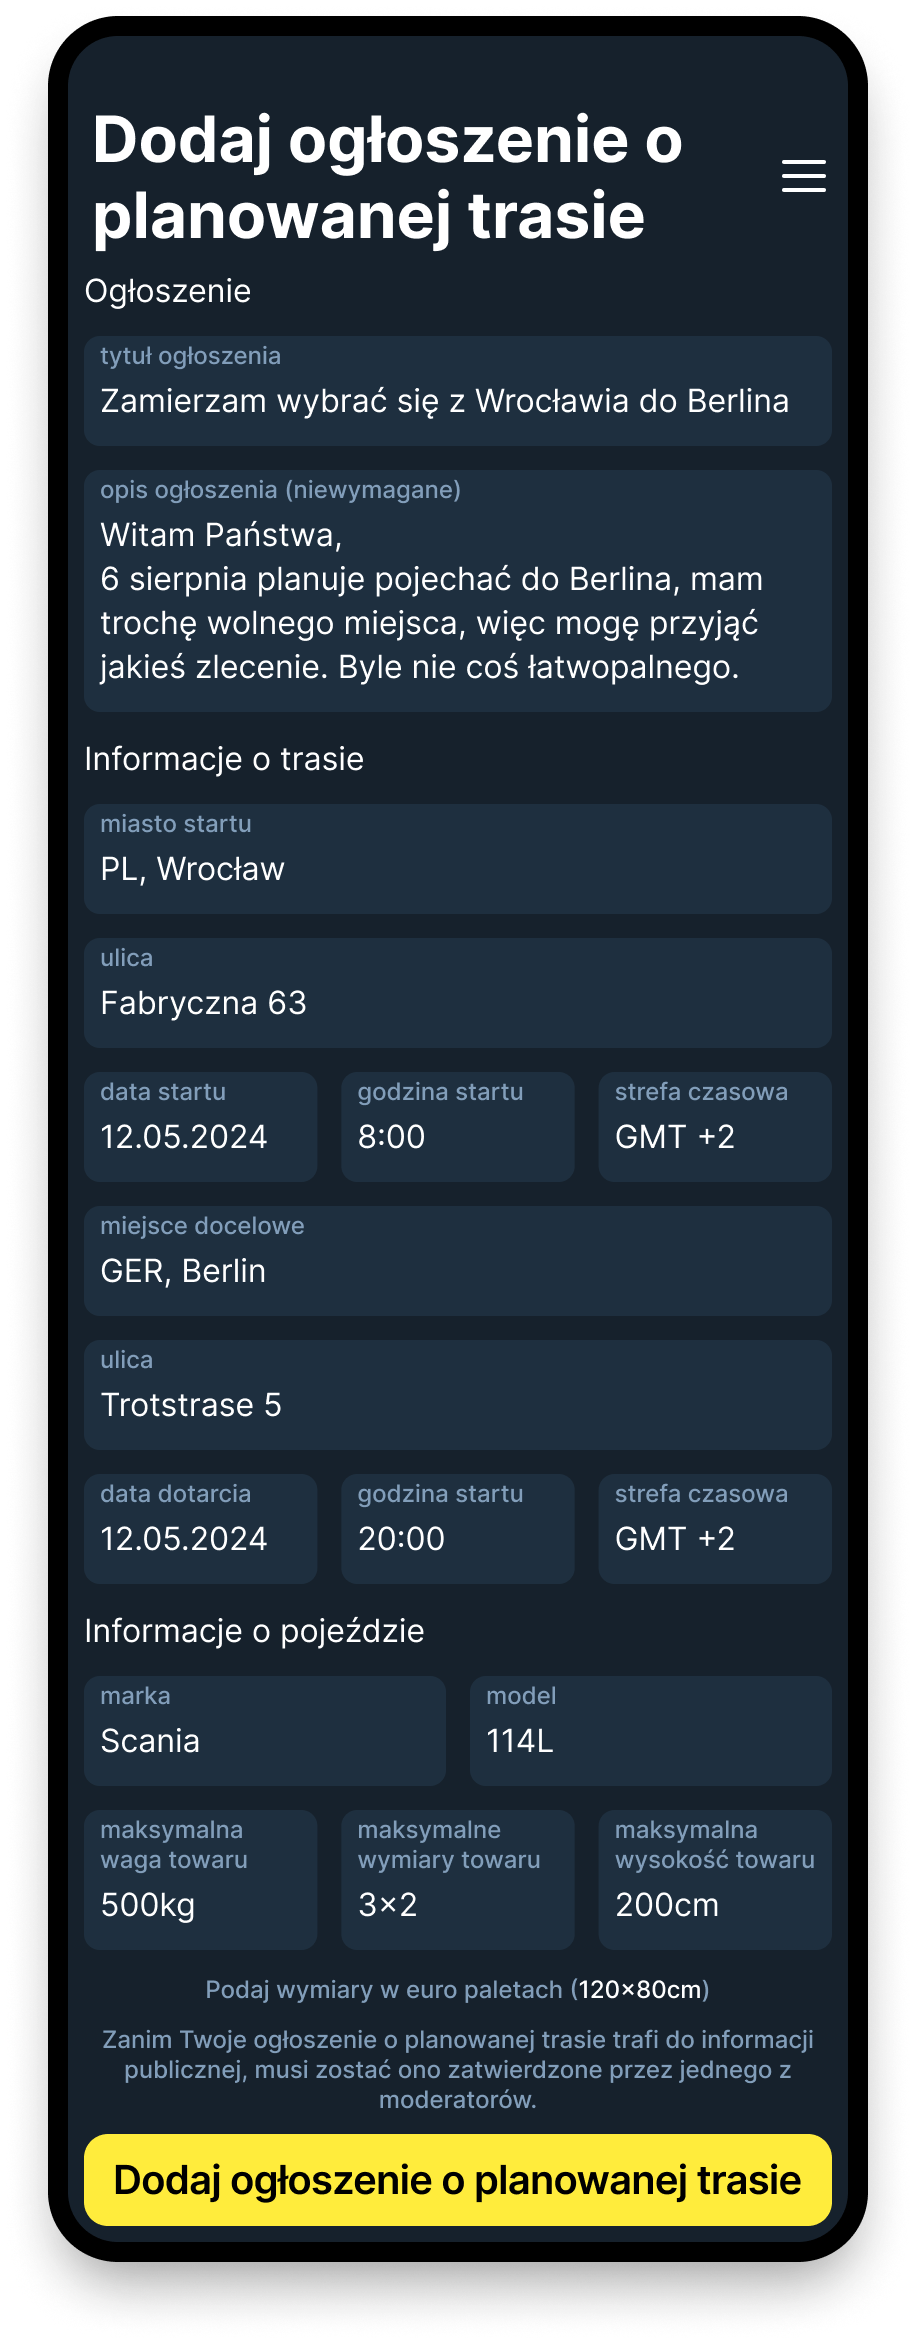
\includegraphics[width=0.3\linewidth]{rozdzial1/nowe_ogloszenie_m.png}}}
    \end{tabular}
    \caption{Dodawanie nowego ogłoszenia o planowanej trasie w wersji mobilnej: a) Menu po zalogowaniu jako przewoźnik b) Formularz dodawania ogłoszenia o planowanej trasie}
	\label{Rys. fig:Dodawanie nowego ogłoszenia o planowanej trasie - ab - mobile}
\end{figure}
\begin{figure}[H]
 \centering
  \begin{tabular}{@{}ccc@{}}
  a) & b)\\
  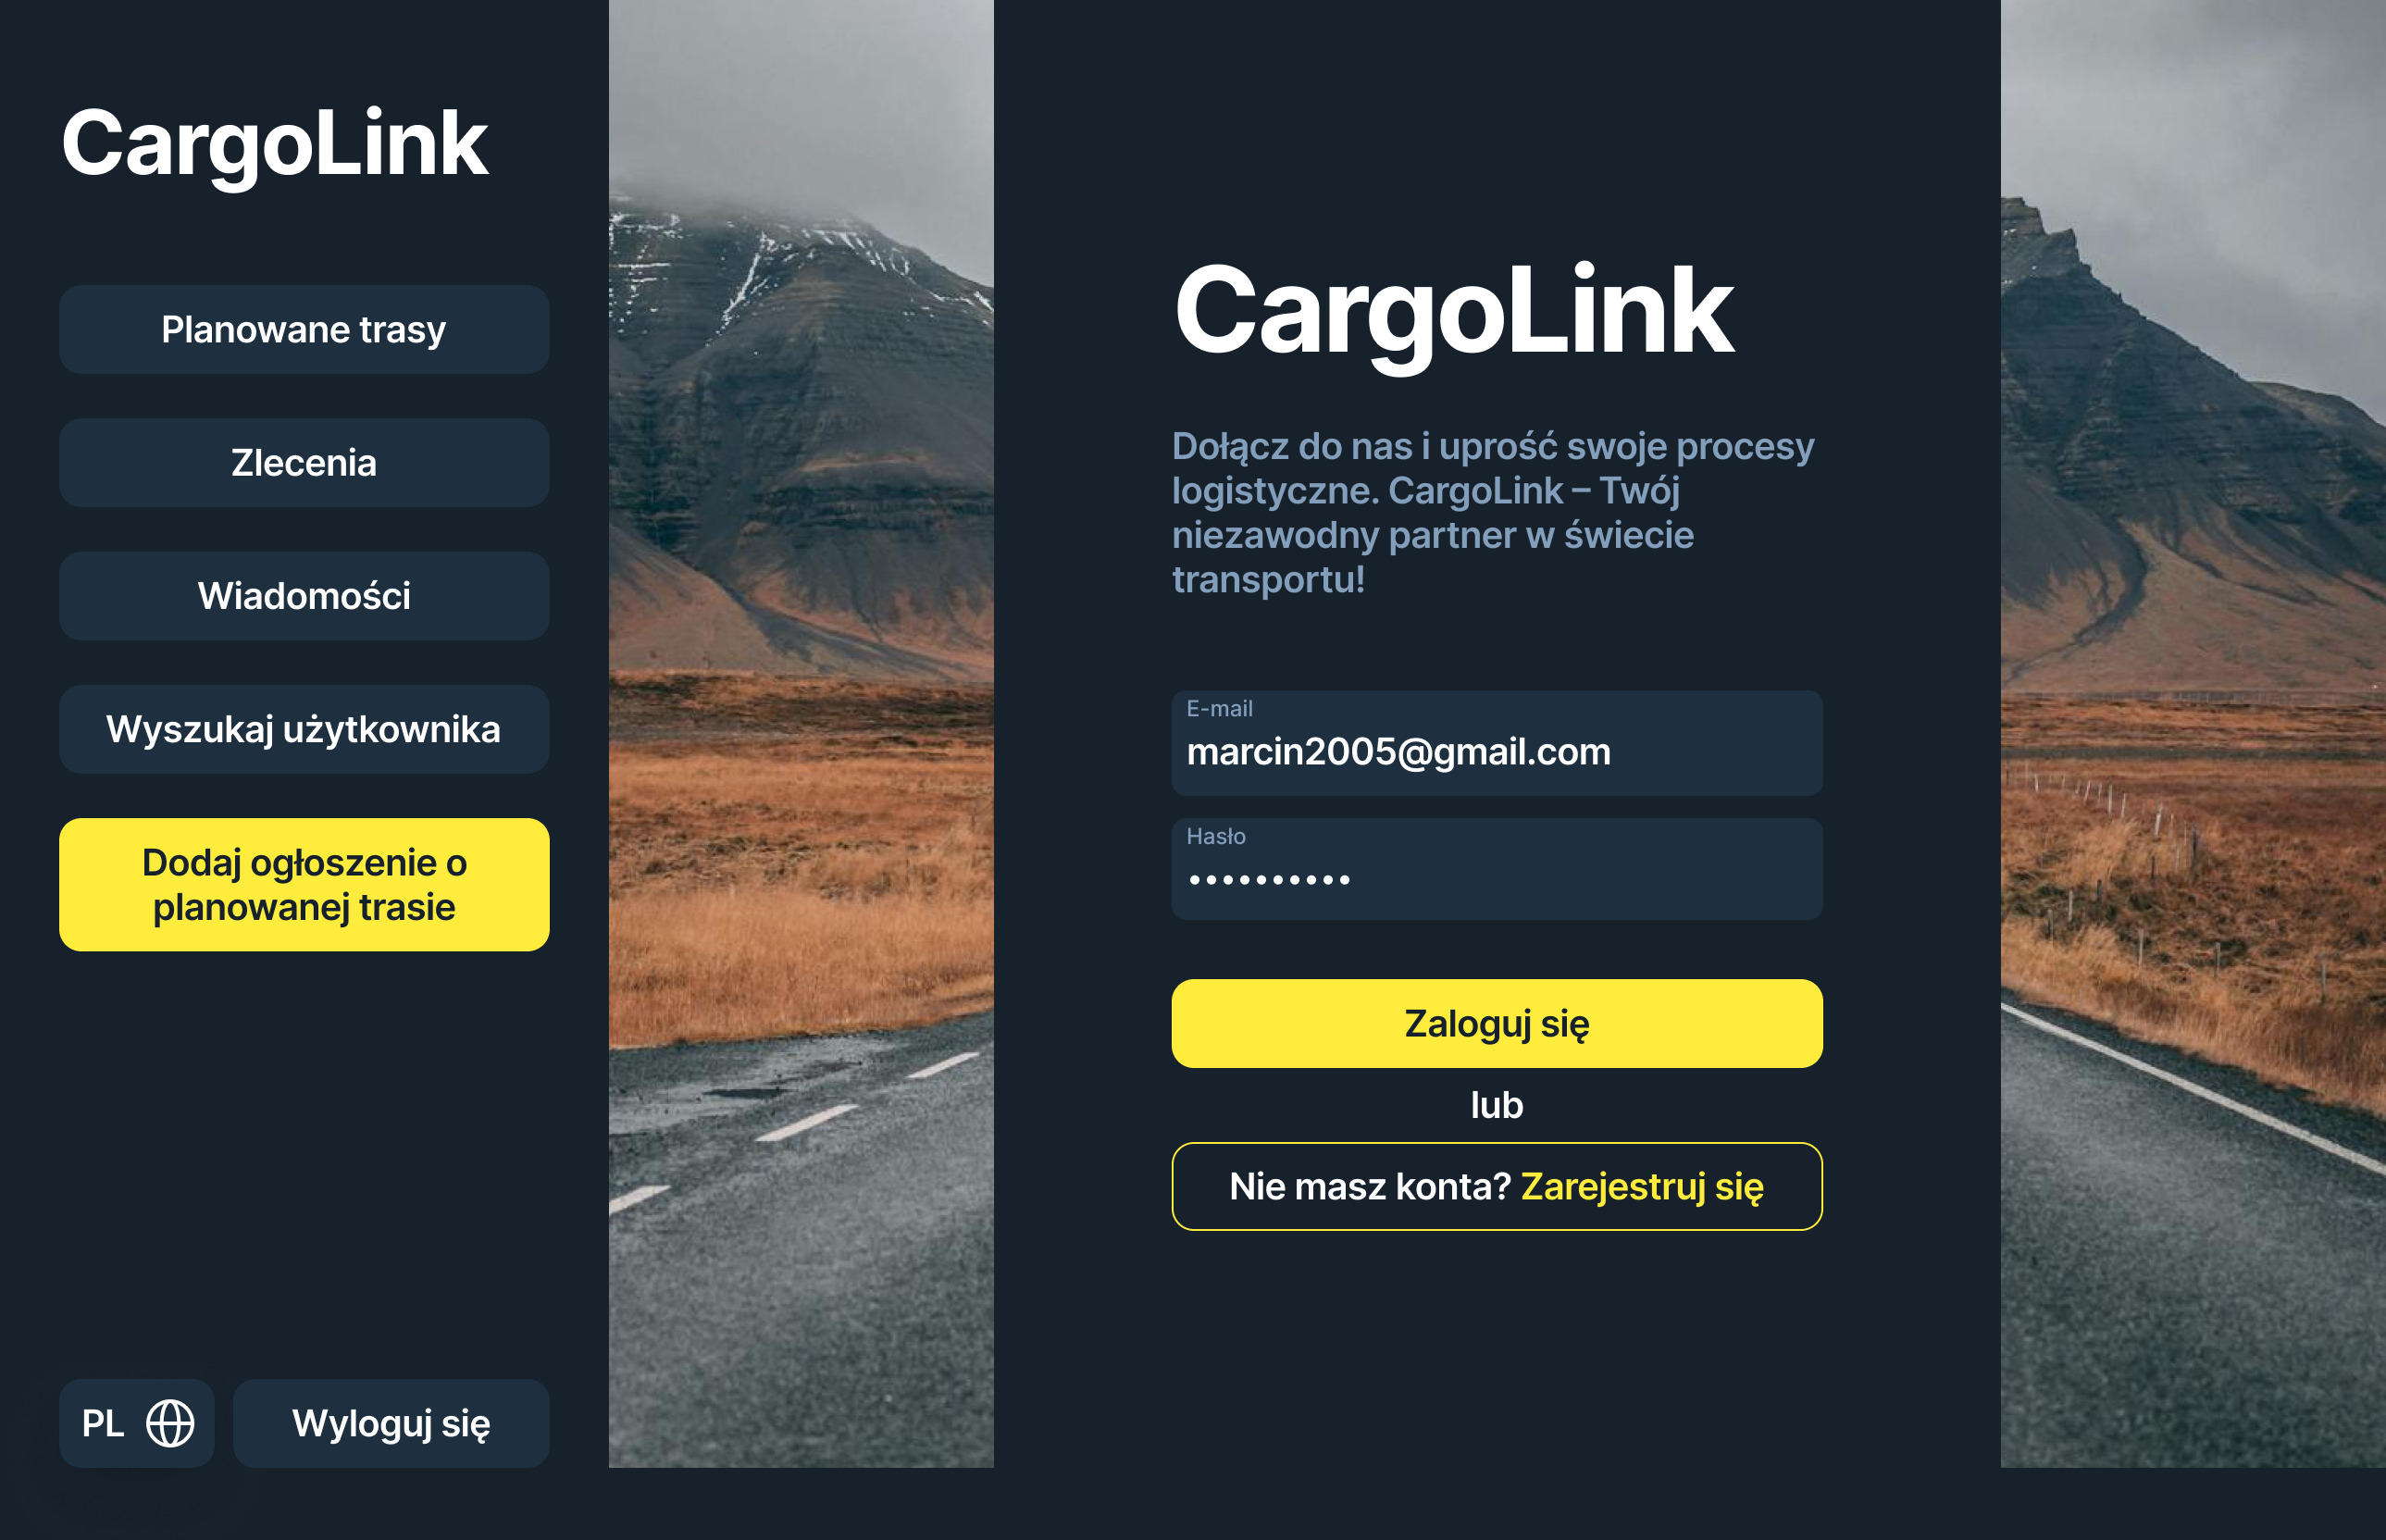
\includegraphics[width=0.45\textwidth]{rozdzial1/menu_d_przewoznik.jpg} &
  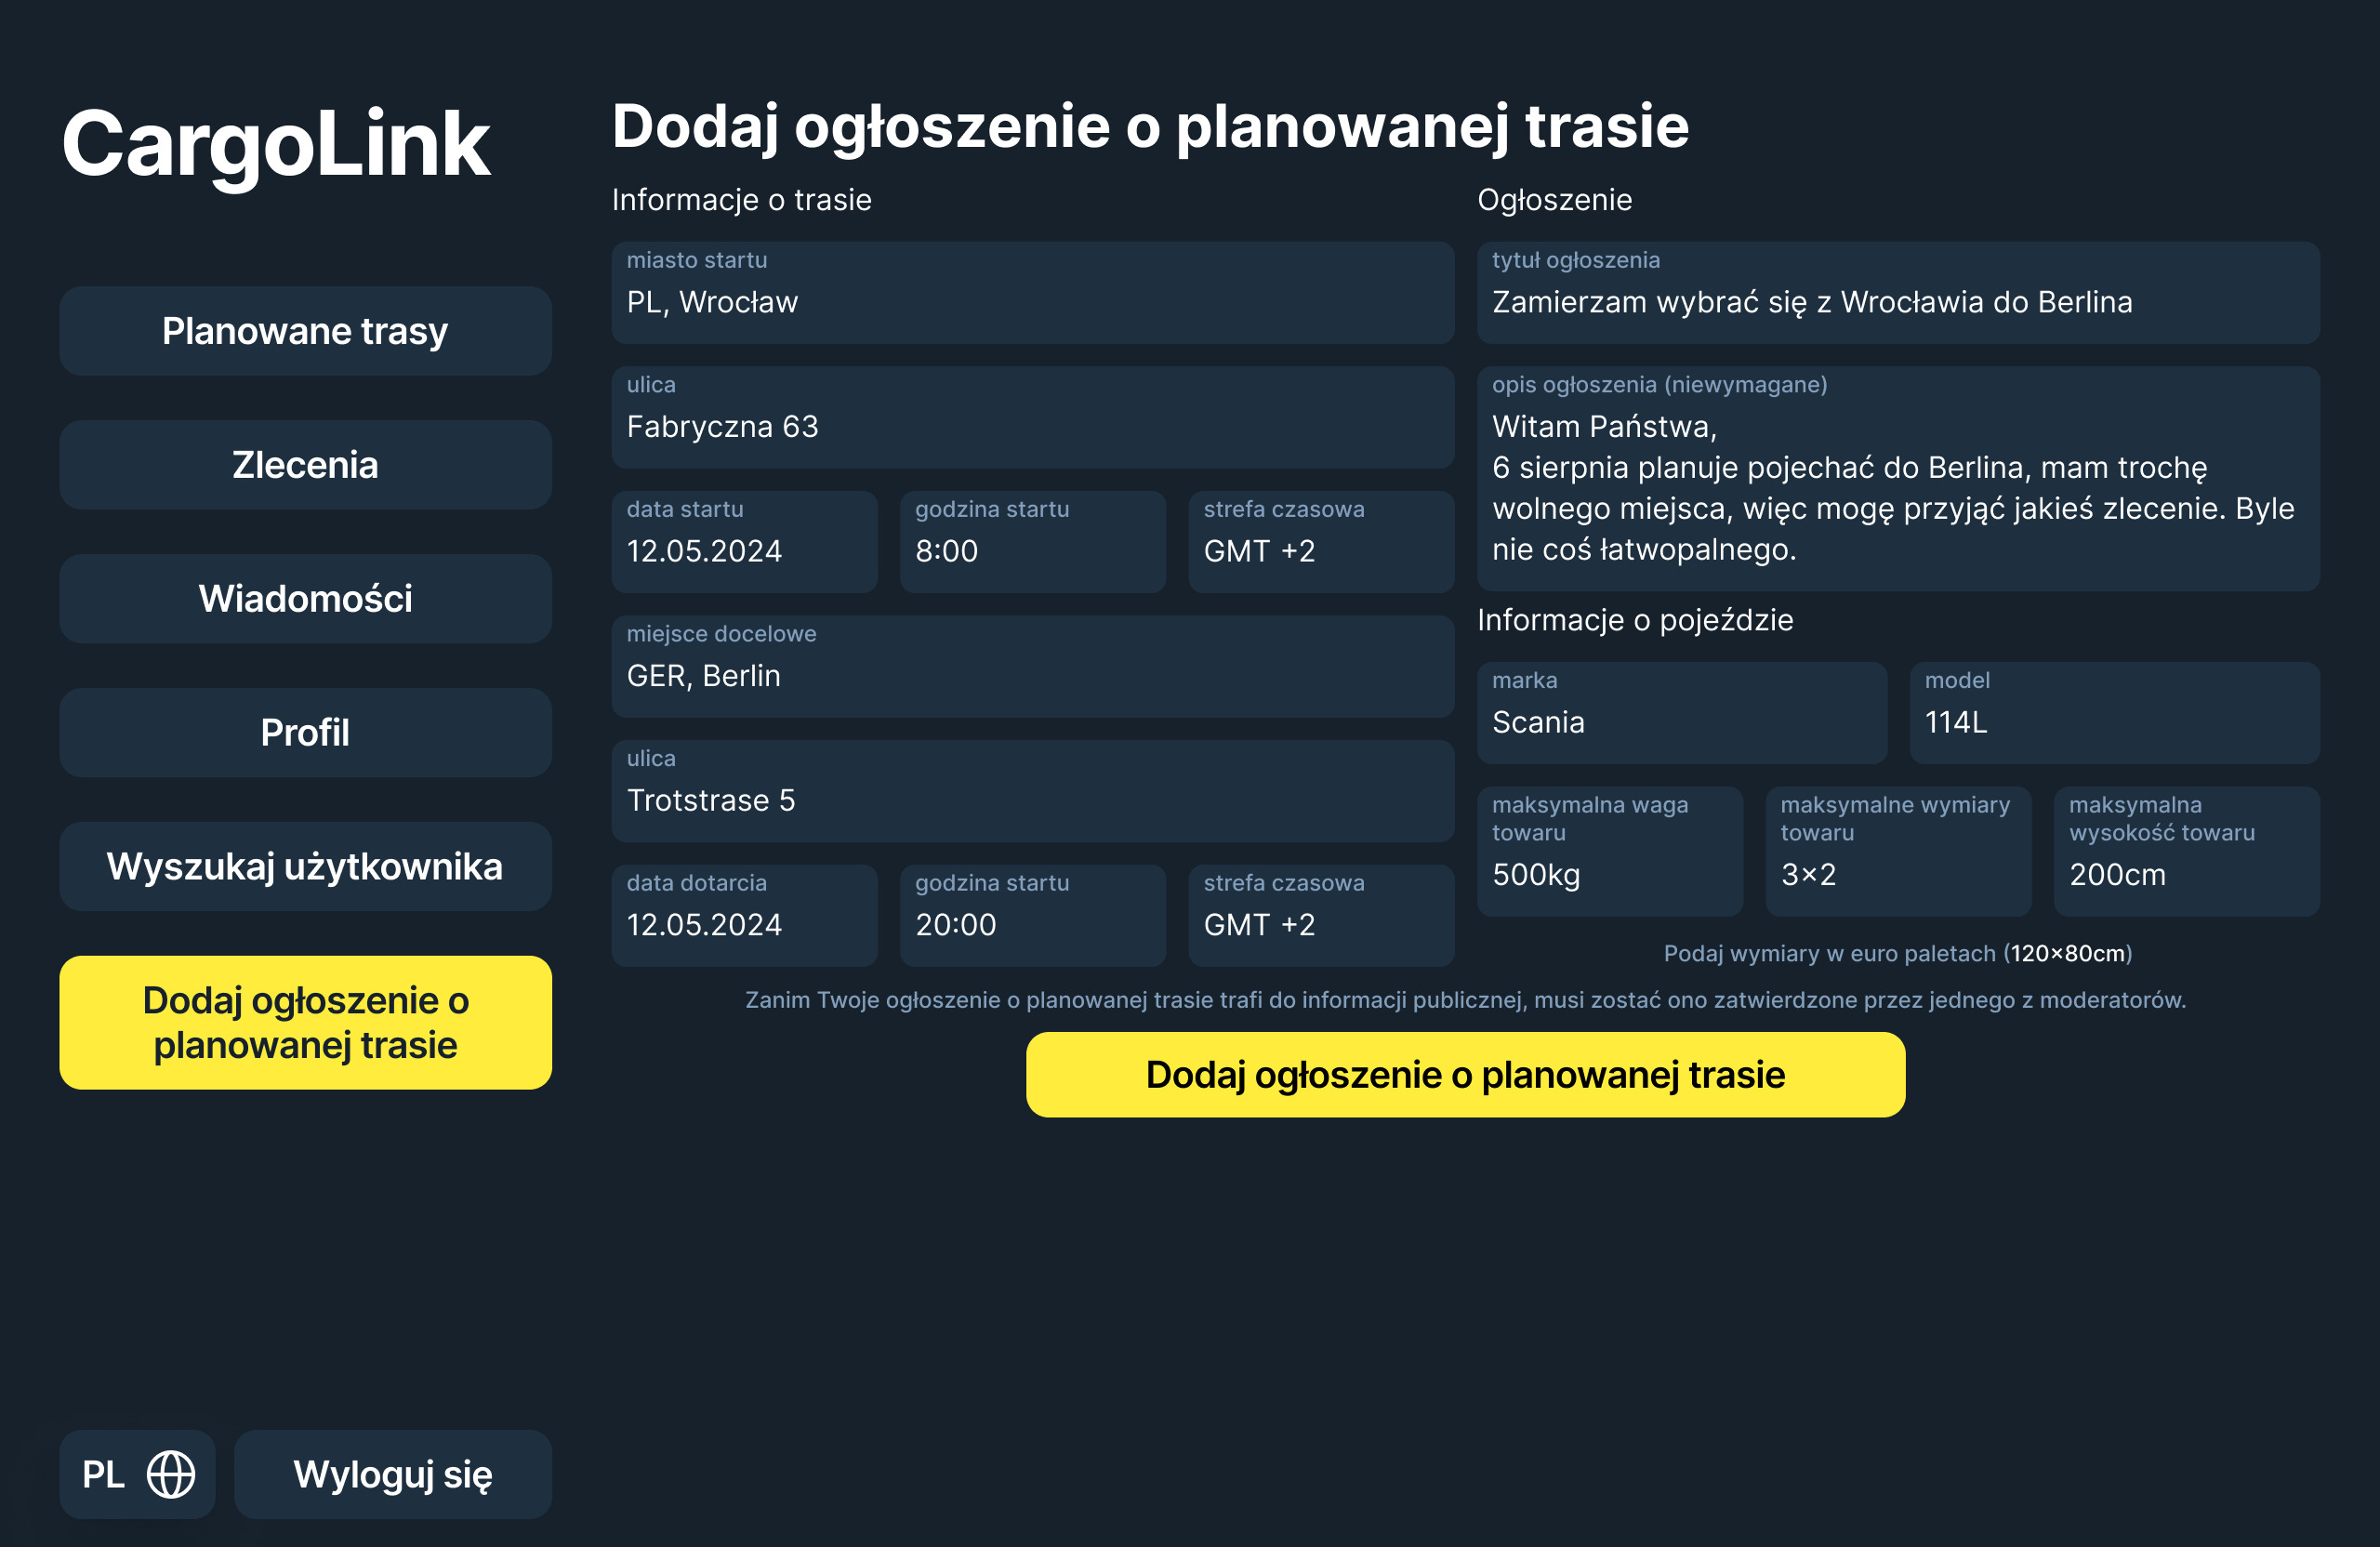
\includegraphics[width=0.45\textwidth]{rozdzial1/nowe_ogloszenie_d.jpg}
  \end{tabular}
 \caption{Dodawanie nowego ogłoszenia o planowanej trasie w wersji desktopowej: a) Menu po zalogowaniu jako przewoźnik b) Formularz dodawania ogłoszenia o planowanej trasie}
 \label{Rys. fig:Dodawanie nowego ogłoszenia o planowanej trasie - ab - desktop}
\end{figure}

\texttt{Otworzenie czatu z innym użytkownikiem} \\
\label{Otworzenie czatu z innym uzytkownikiem}
Zdarzenie inicjujące: Kliknięcie w przycisk \texttt{Przejdź do czatu} (Rys. \ref{Rys. fig:Wyświetlenie ogłoszenia - ab - mobile}.a lub \ref{Rys. fig:Wyświetlenie ogłoszenia - ab - mobile}.b lub \ref{Rys. fig:Wyświetlenie ogłoszenia - ab - desktop}.a lub \ref{Rys. fig:Wyświetlenie ogłoszenia - ab - desktop}.b) \\
Warunki początkowe: Bycie zalogowanym. \\
Przebieg podstawowy realizacji przypadku użycia:
\begin{enumerate}
    \item Kliknięcie w przycisk \texttt{Przejdź do czatu} (Rys. \ref{Rys. fig:Wyświetlenie ogłoszenia - ab - mobile}.a lub \ref{Rys. fig:Wyświetlenie ogłoszenia - ab - mobile}.b lub \ref{Rys. fig:Wyświetlenie ogłoszenia - ab - desktop}.a lub \ref{Rys. fig:Wyświetlenie ogłoszenia - ab - desktop}.b);
    \item Otworzenie czatu z autorem ogłoszenia (Rys. \ref{Rys. fig:Czat - mobile}.b lub \ref{Rys. fig:Czat - desktop}).
\end{enumerate}
Warunki końcowe: Użytkownik przechodzi do konwersacji z wybranym użytkownikiem (Rys. \ref{Rys. fig:Czat - mobile}.b lub \ref{Rys. fig:Czat - desktop})).\\
Przebieg alternatywny realizacji przypadku użycia: \begin{enumerate}
    \item Kliknięcie w przycisk \texttt{Wiadomości} (Rys. \ref{Rys. fig:Menu nawigacji po aplikacji - ab}.a lub \ref{Rys. fig:Wyświetlenie ogłoszenia - ab - mobile}.b lub \ref{Rys. fig:Wyświetlenie ogłoszenia - ab - desktop}.a lub \ref{Rys. fig:Wyświetlenie ogłoszenia - ab - desktop}.b);
    \item Otworzenie czatu z autorem ogłoszenia (Rys. \ref{Rys. fig:Czat - mobile}.b lub \ref{Rys. fig:Czat - desktop}).
\end{enumerate}
\begin{figure}[H]
	\centering
	\begin{tabular}{@{}ccc@{}}
            a) & b)\\
    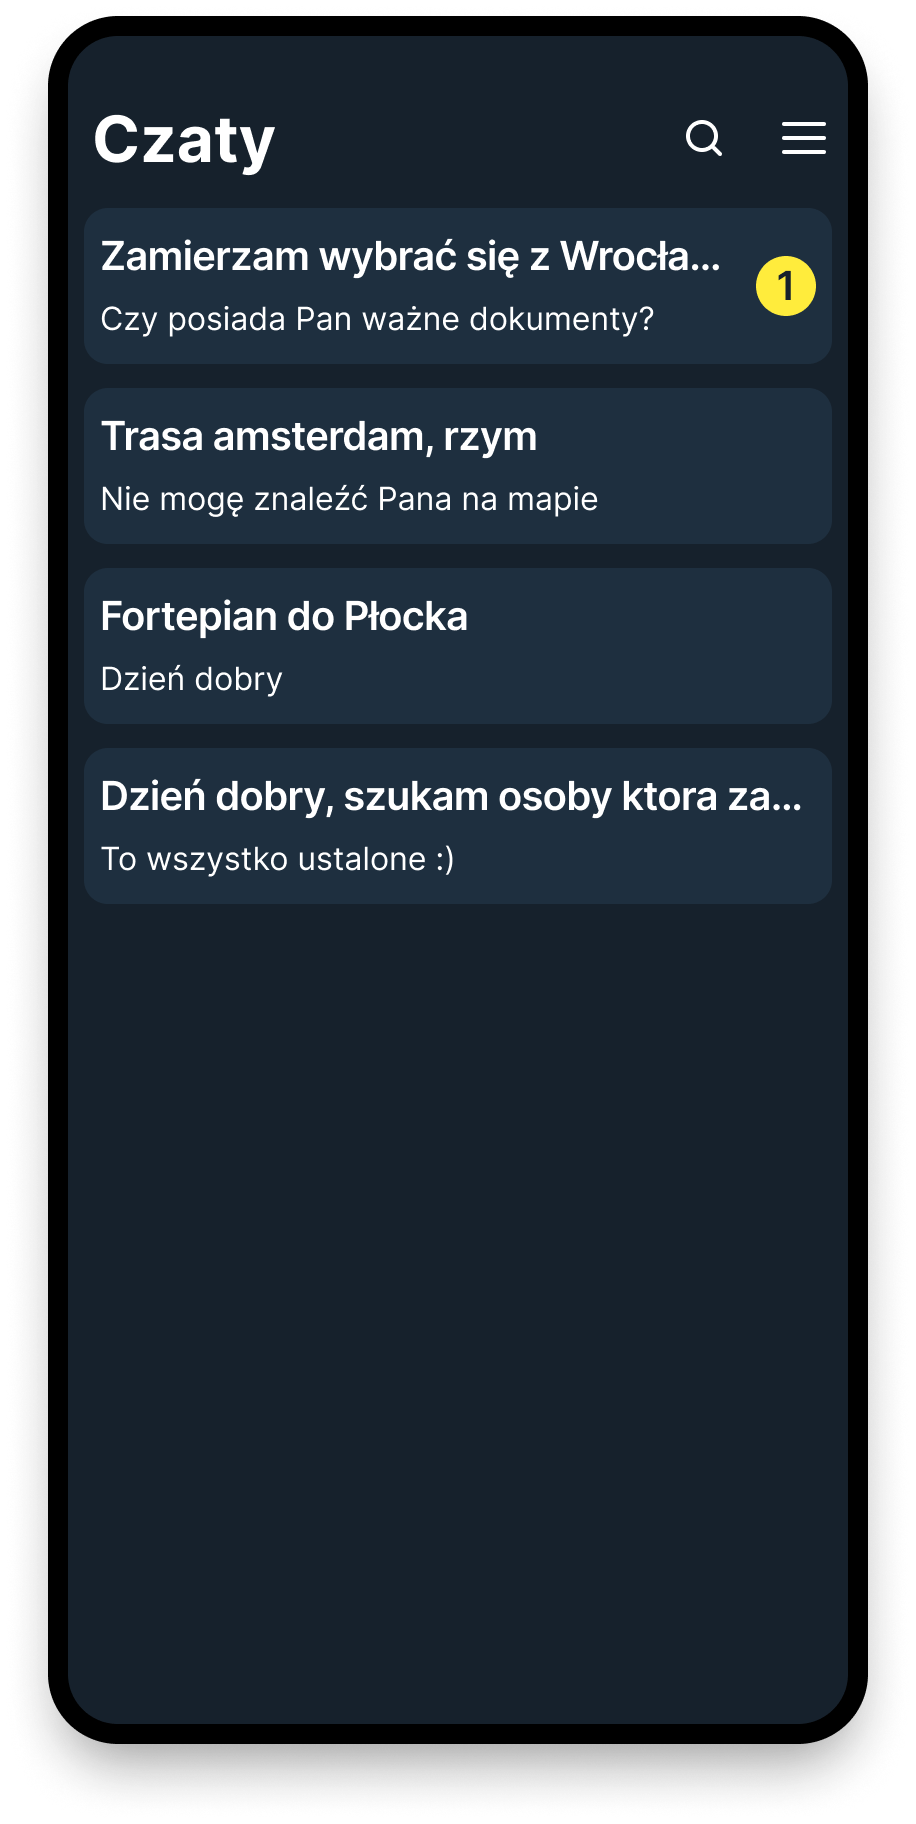
\includegraphics[width=0.3\linewidth]{rozdzial1/czat_1_m.png} &
    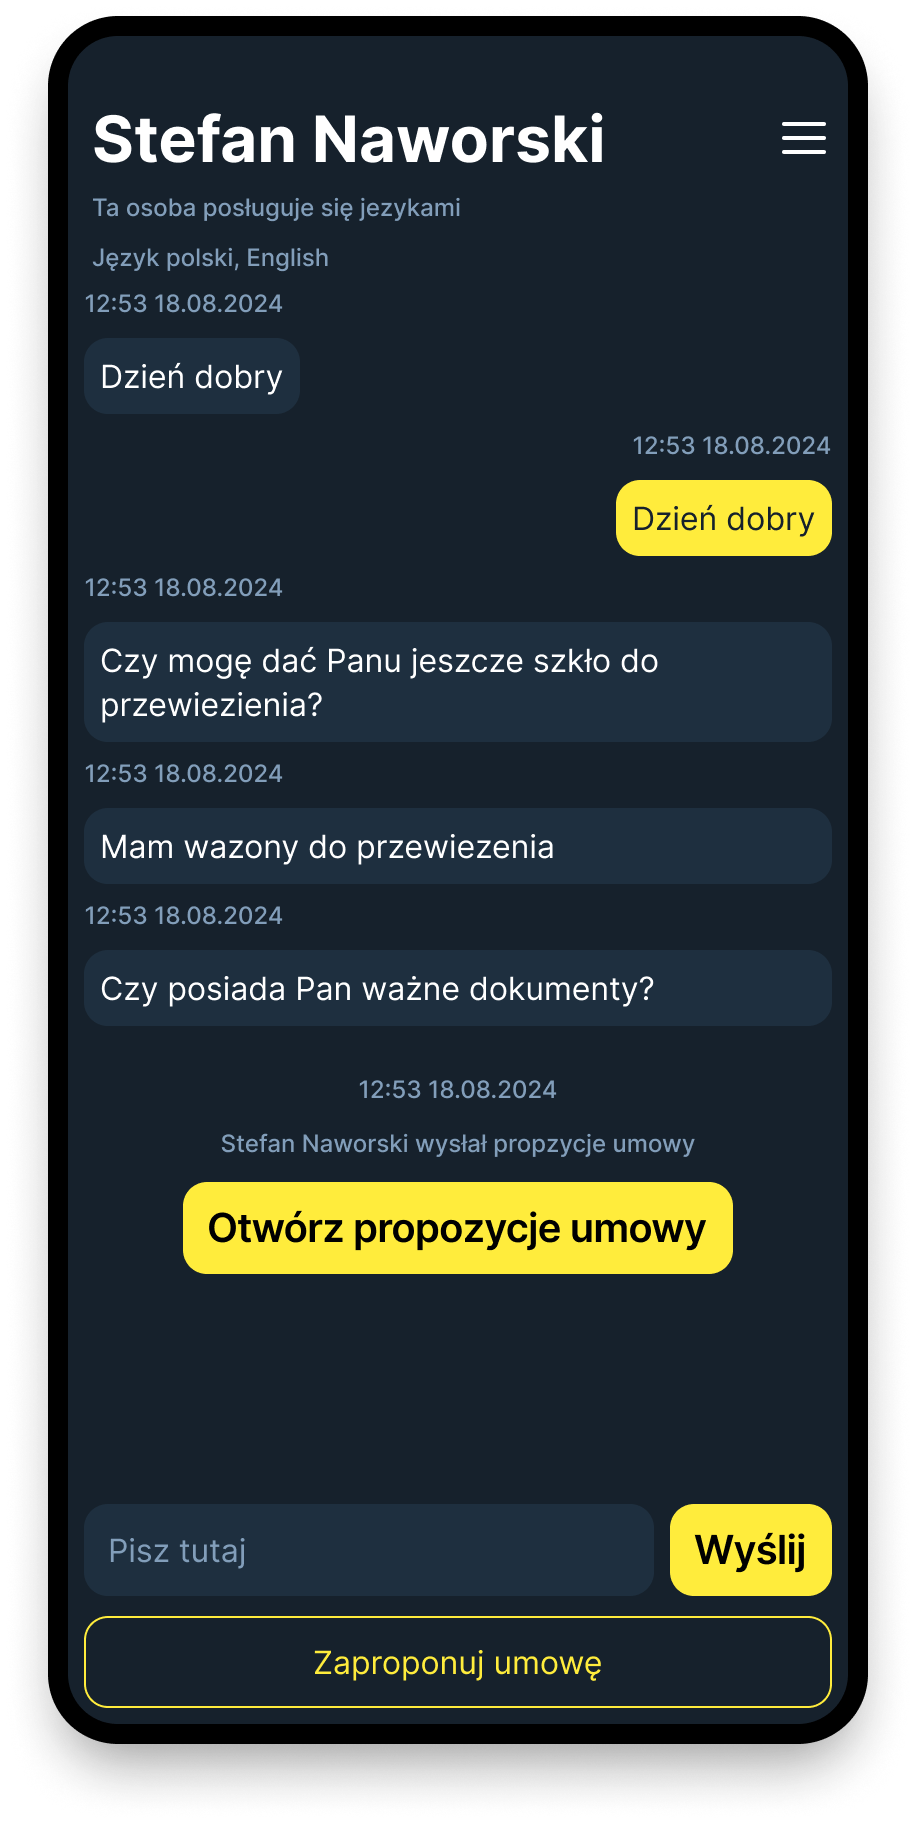
\includegraphics[width=0.3\linewidth]{rozdzial1/czat_2_m.png}
    \end{tabular}
    \caption{Czat w wersji mobilnej: a) Menu wyboru konwersacji, b) Czat}
	\label{Rys. fig:Czat - mobile}
\end{figure}
\begin{figure}[H]
	\centering
		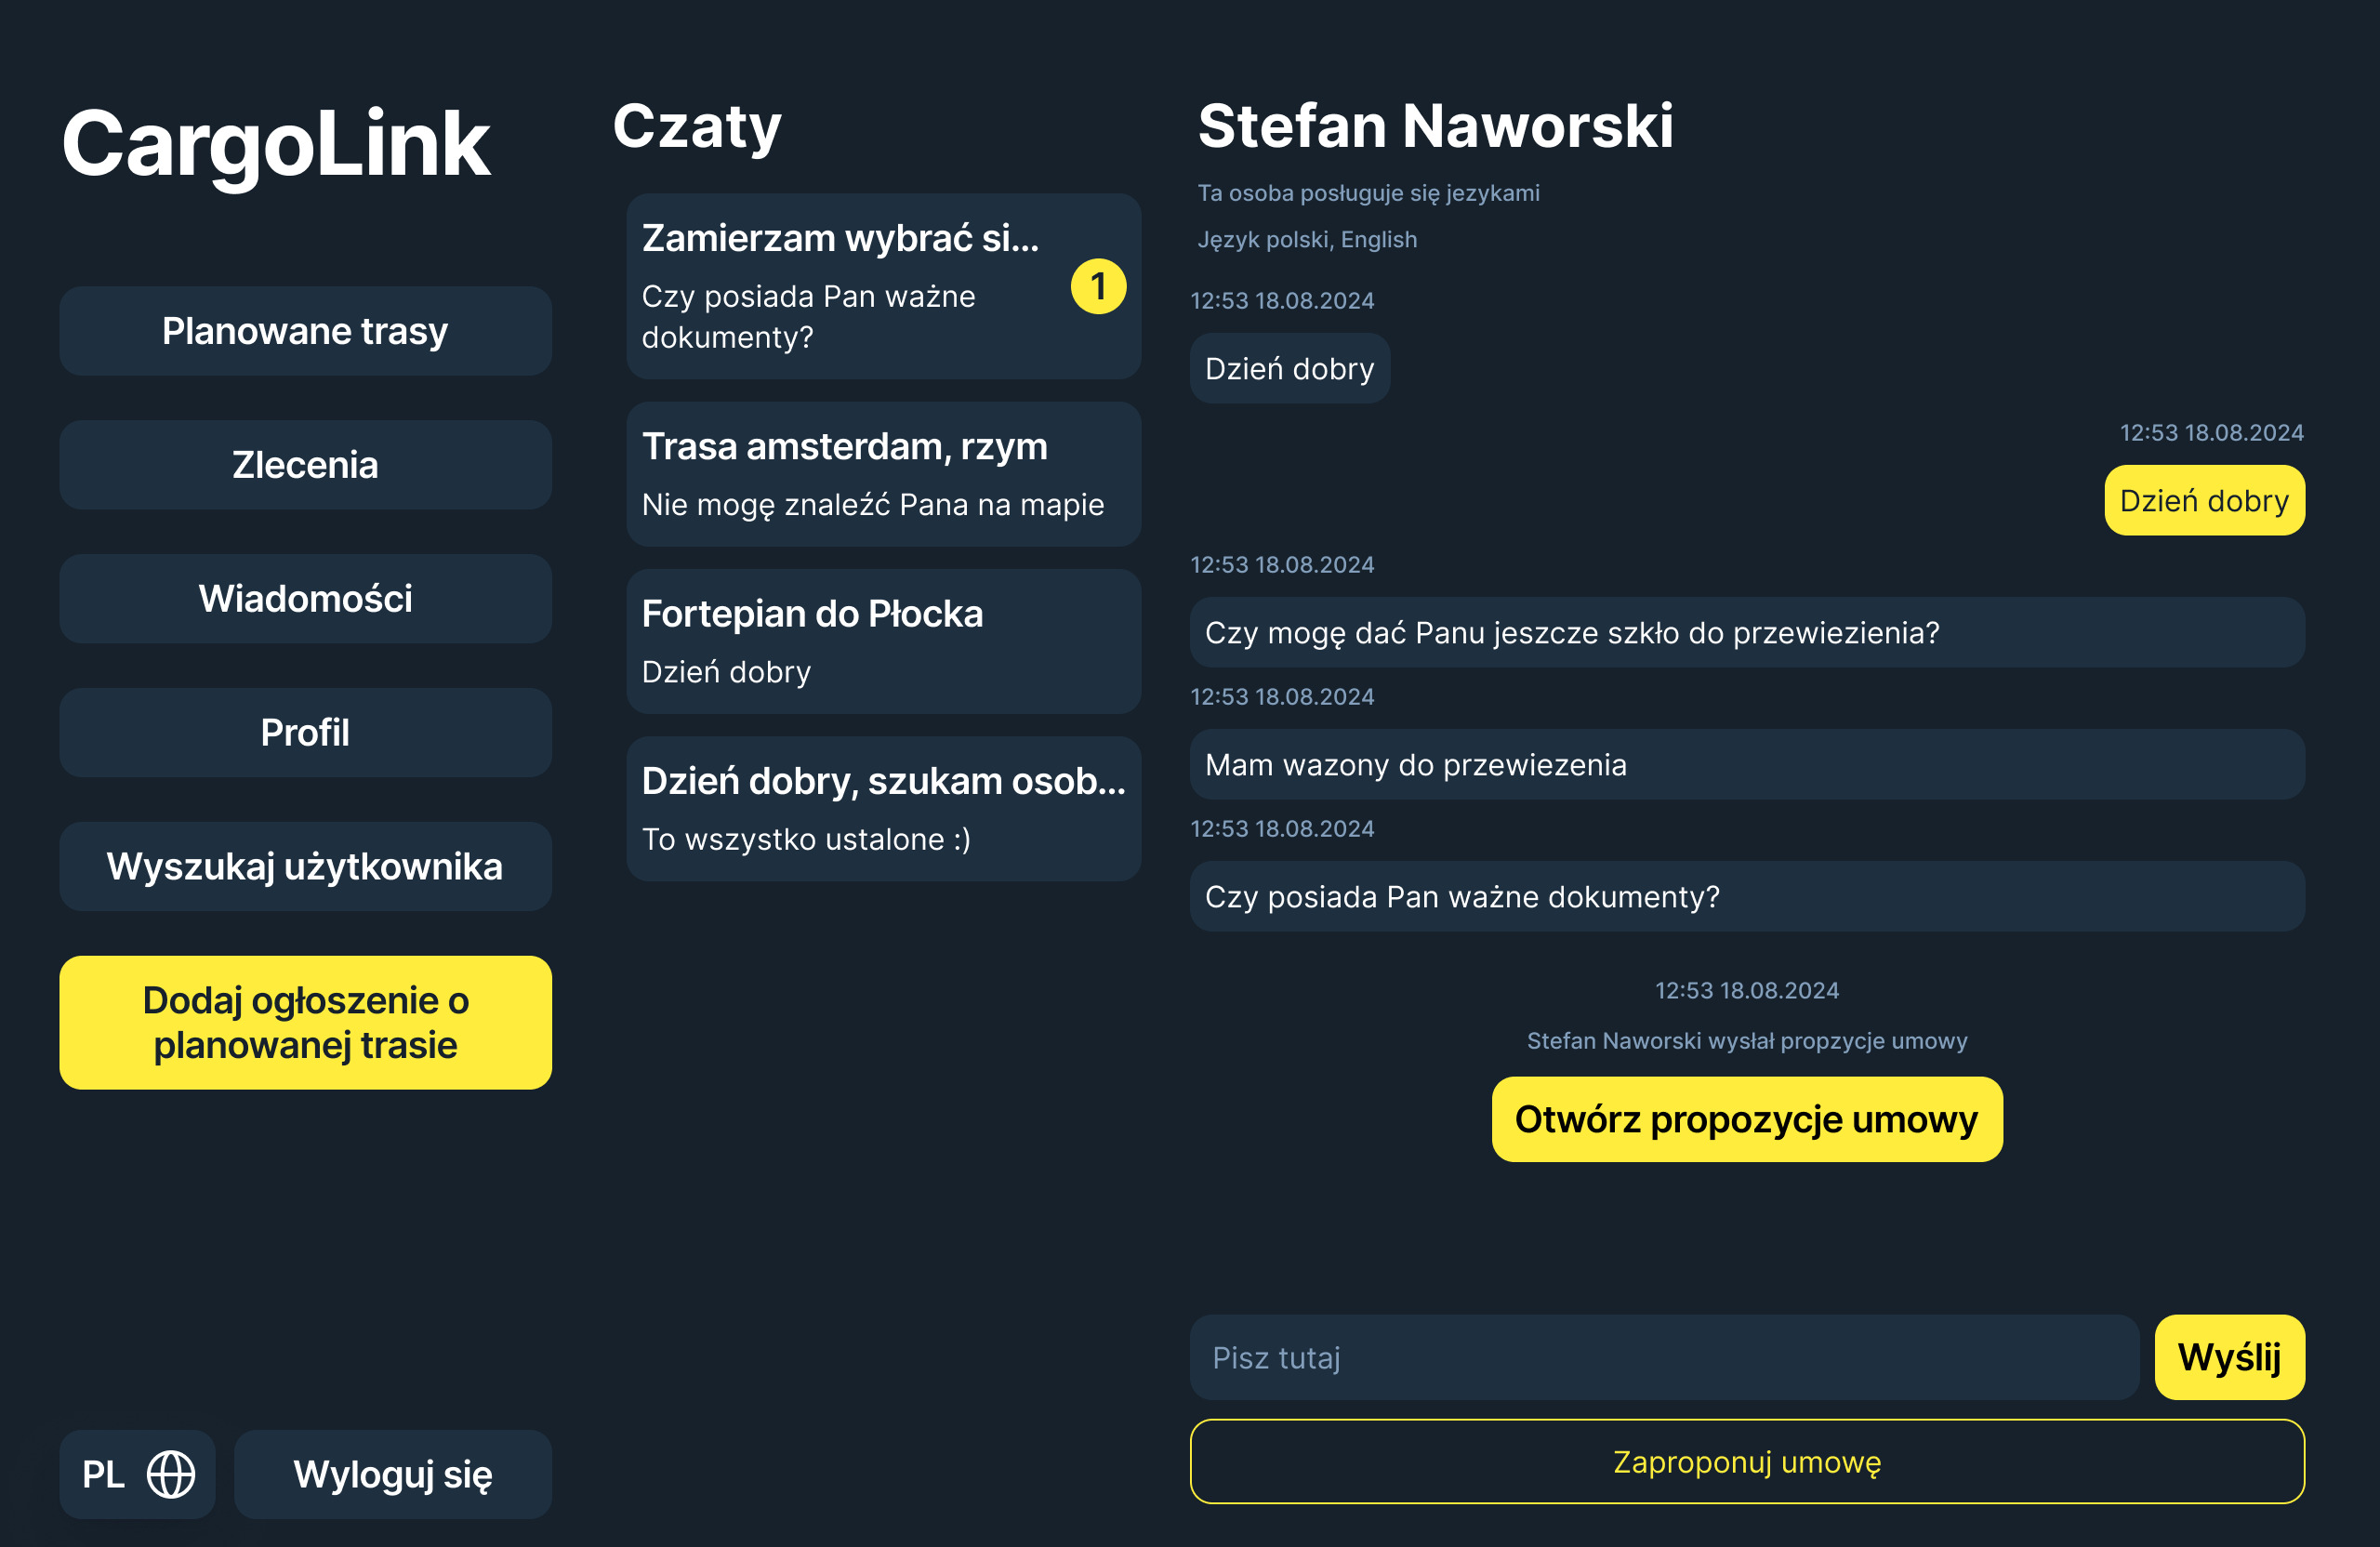
\includegraphics[width=0.7\linewidth]{rozdzial1/czat_d.jpg}
	\caption{Czat w wersji desktopowej}
	\label{Rys. fig:Czat - desktop}
\end{figure}

\texttt{Wysłanie propozycji umowy} \\
Zdarzenie inicjujące: Kliknięcie przycisku \texttt{Zaproponuj umowę}. \\
Warunki początkowe: Użytkownik jest zalogowany.\\
Przebieg podstawowy realizacji przypadku użycia:\\
\begin{enumerate}
    \item Wykonanie przypadku użycia \ref{Otworzenie czatu z innym uzytkownikiem};
    \item Kliknięcie przycisku \texttt{Zaproponuj umowę} (Rys. \ref{Rys. fig:Czat - mobile}.b lub \ref{Rys. fig:Czat - desktop});
    \item Wypełnienie formularza (Rys. \ref{Rys. fig:Wygeneruj umowe - mobile} lub \ref{Rys. fig:Wygeneruj umowe - desktop});
    \item System sprawdza poprawność wprowadzonych danych;
    \item System wysyła propozycje umowy do rozmówcy.
\end{enumerate}
Warunki końcowe: System wysyła propozycje umowy do rozmówcy.\\
Przebieg alternatywny w realizacji podpunktu (4a): Wprowadzone przez użytkownika dane są nieprawidłowe, system informuje o błędach w formularzu.\\
\begin{figure}[H]
	\centering
		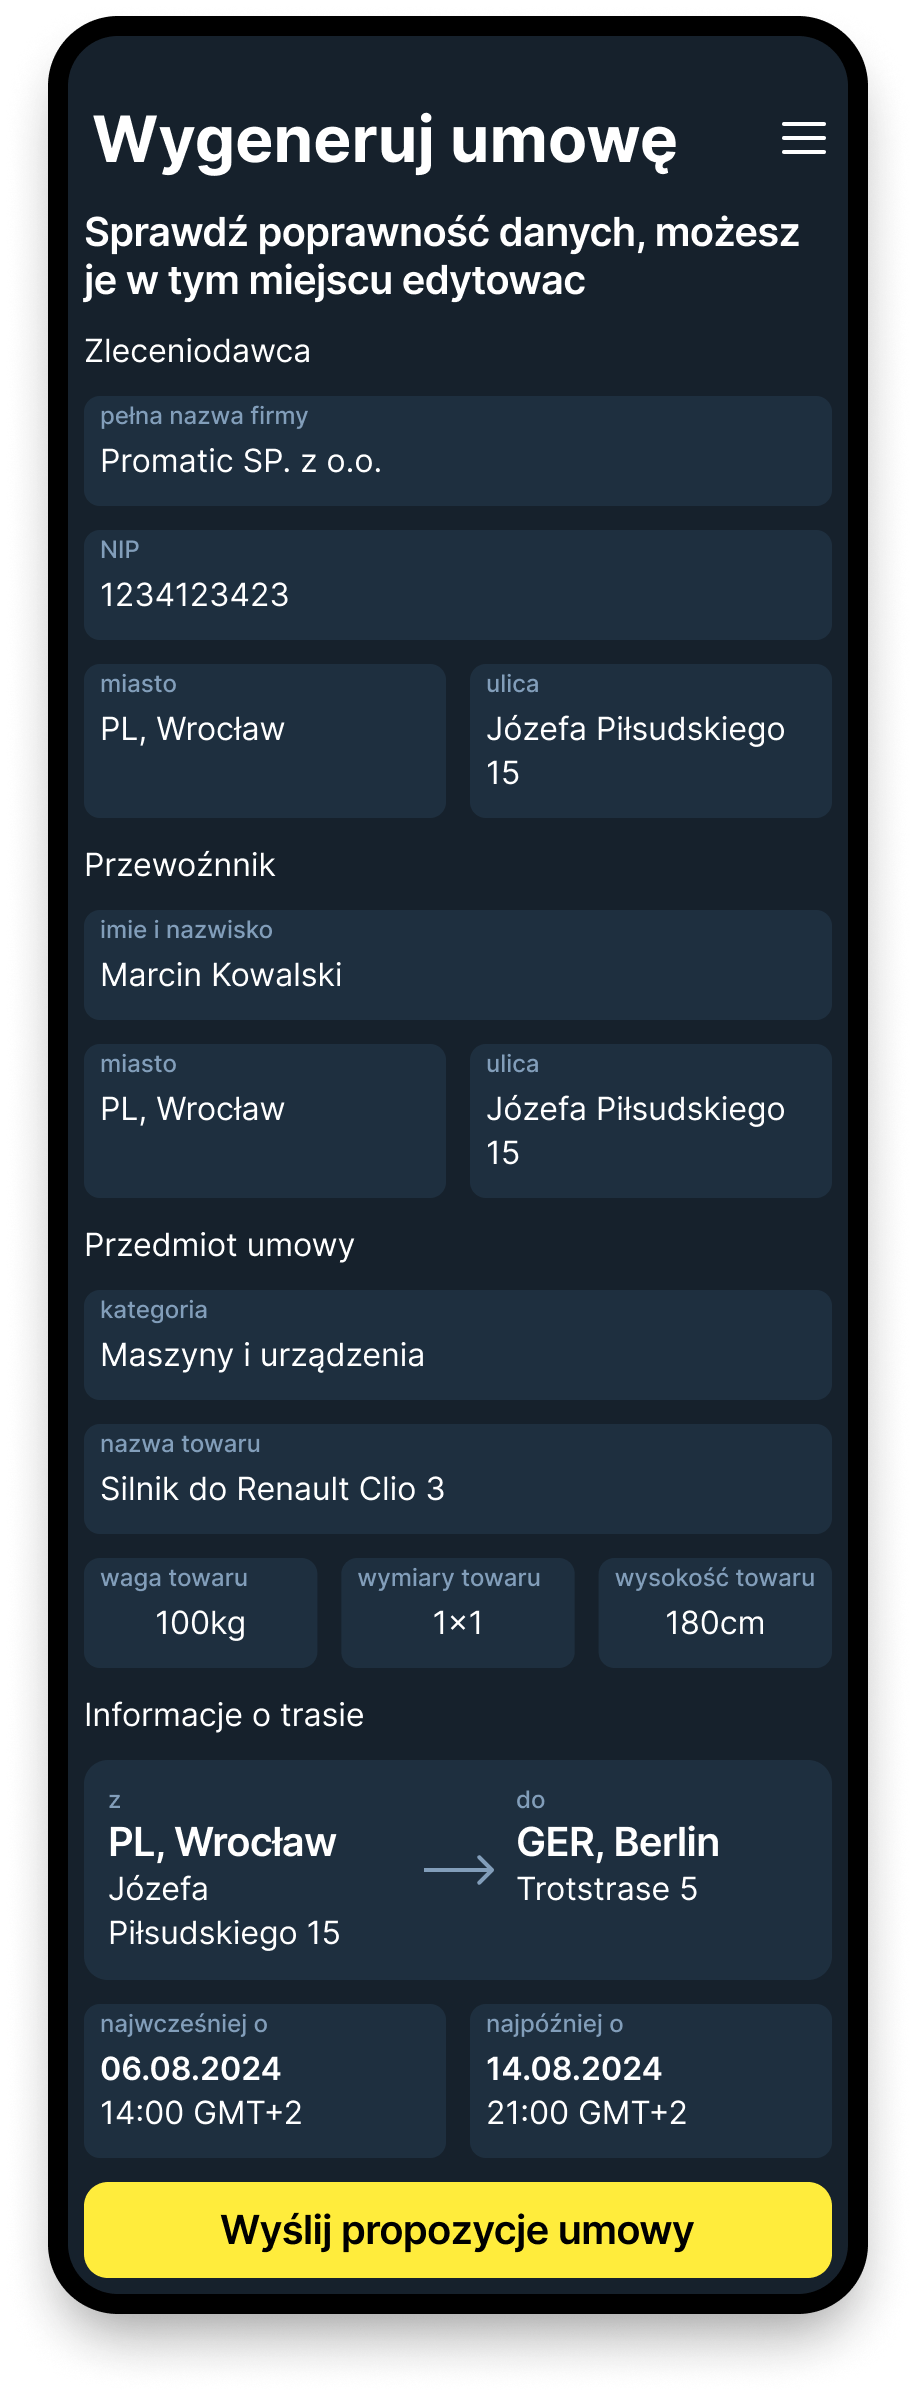
\includegraphics[width=0.3\linewidth]{rozdzial1/wygneruj_umowe_m.png}
	\caption{Formularz generujący umowę w wersji mobilnej}
	\label{Rys. fig:Wygeneruj umowe - mobile}
\end{figure}
\begin{figure}[H]
	\centering
		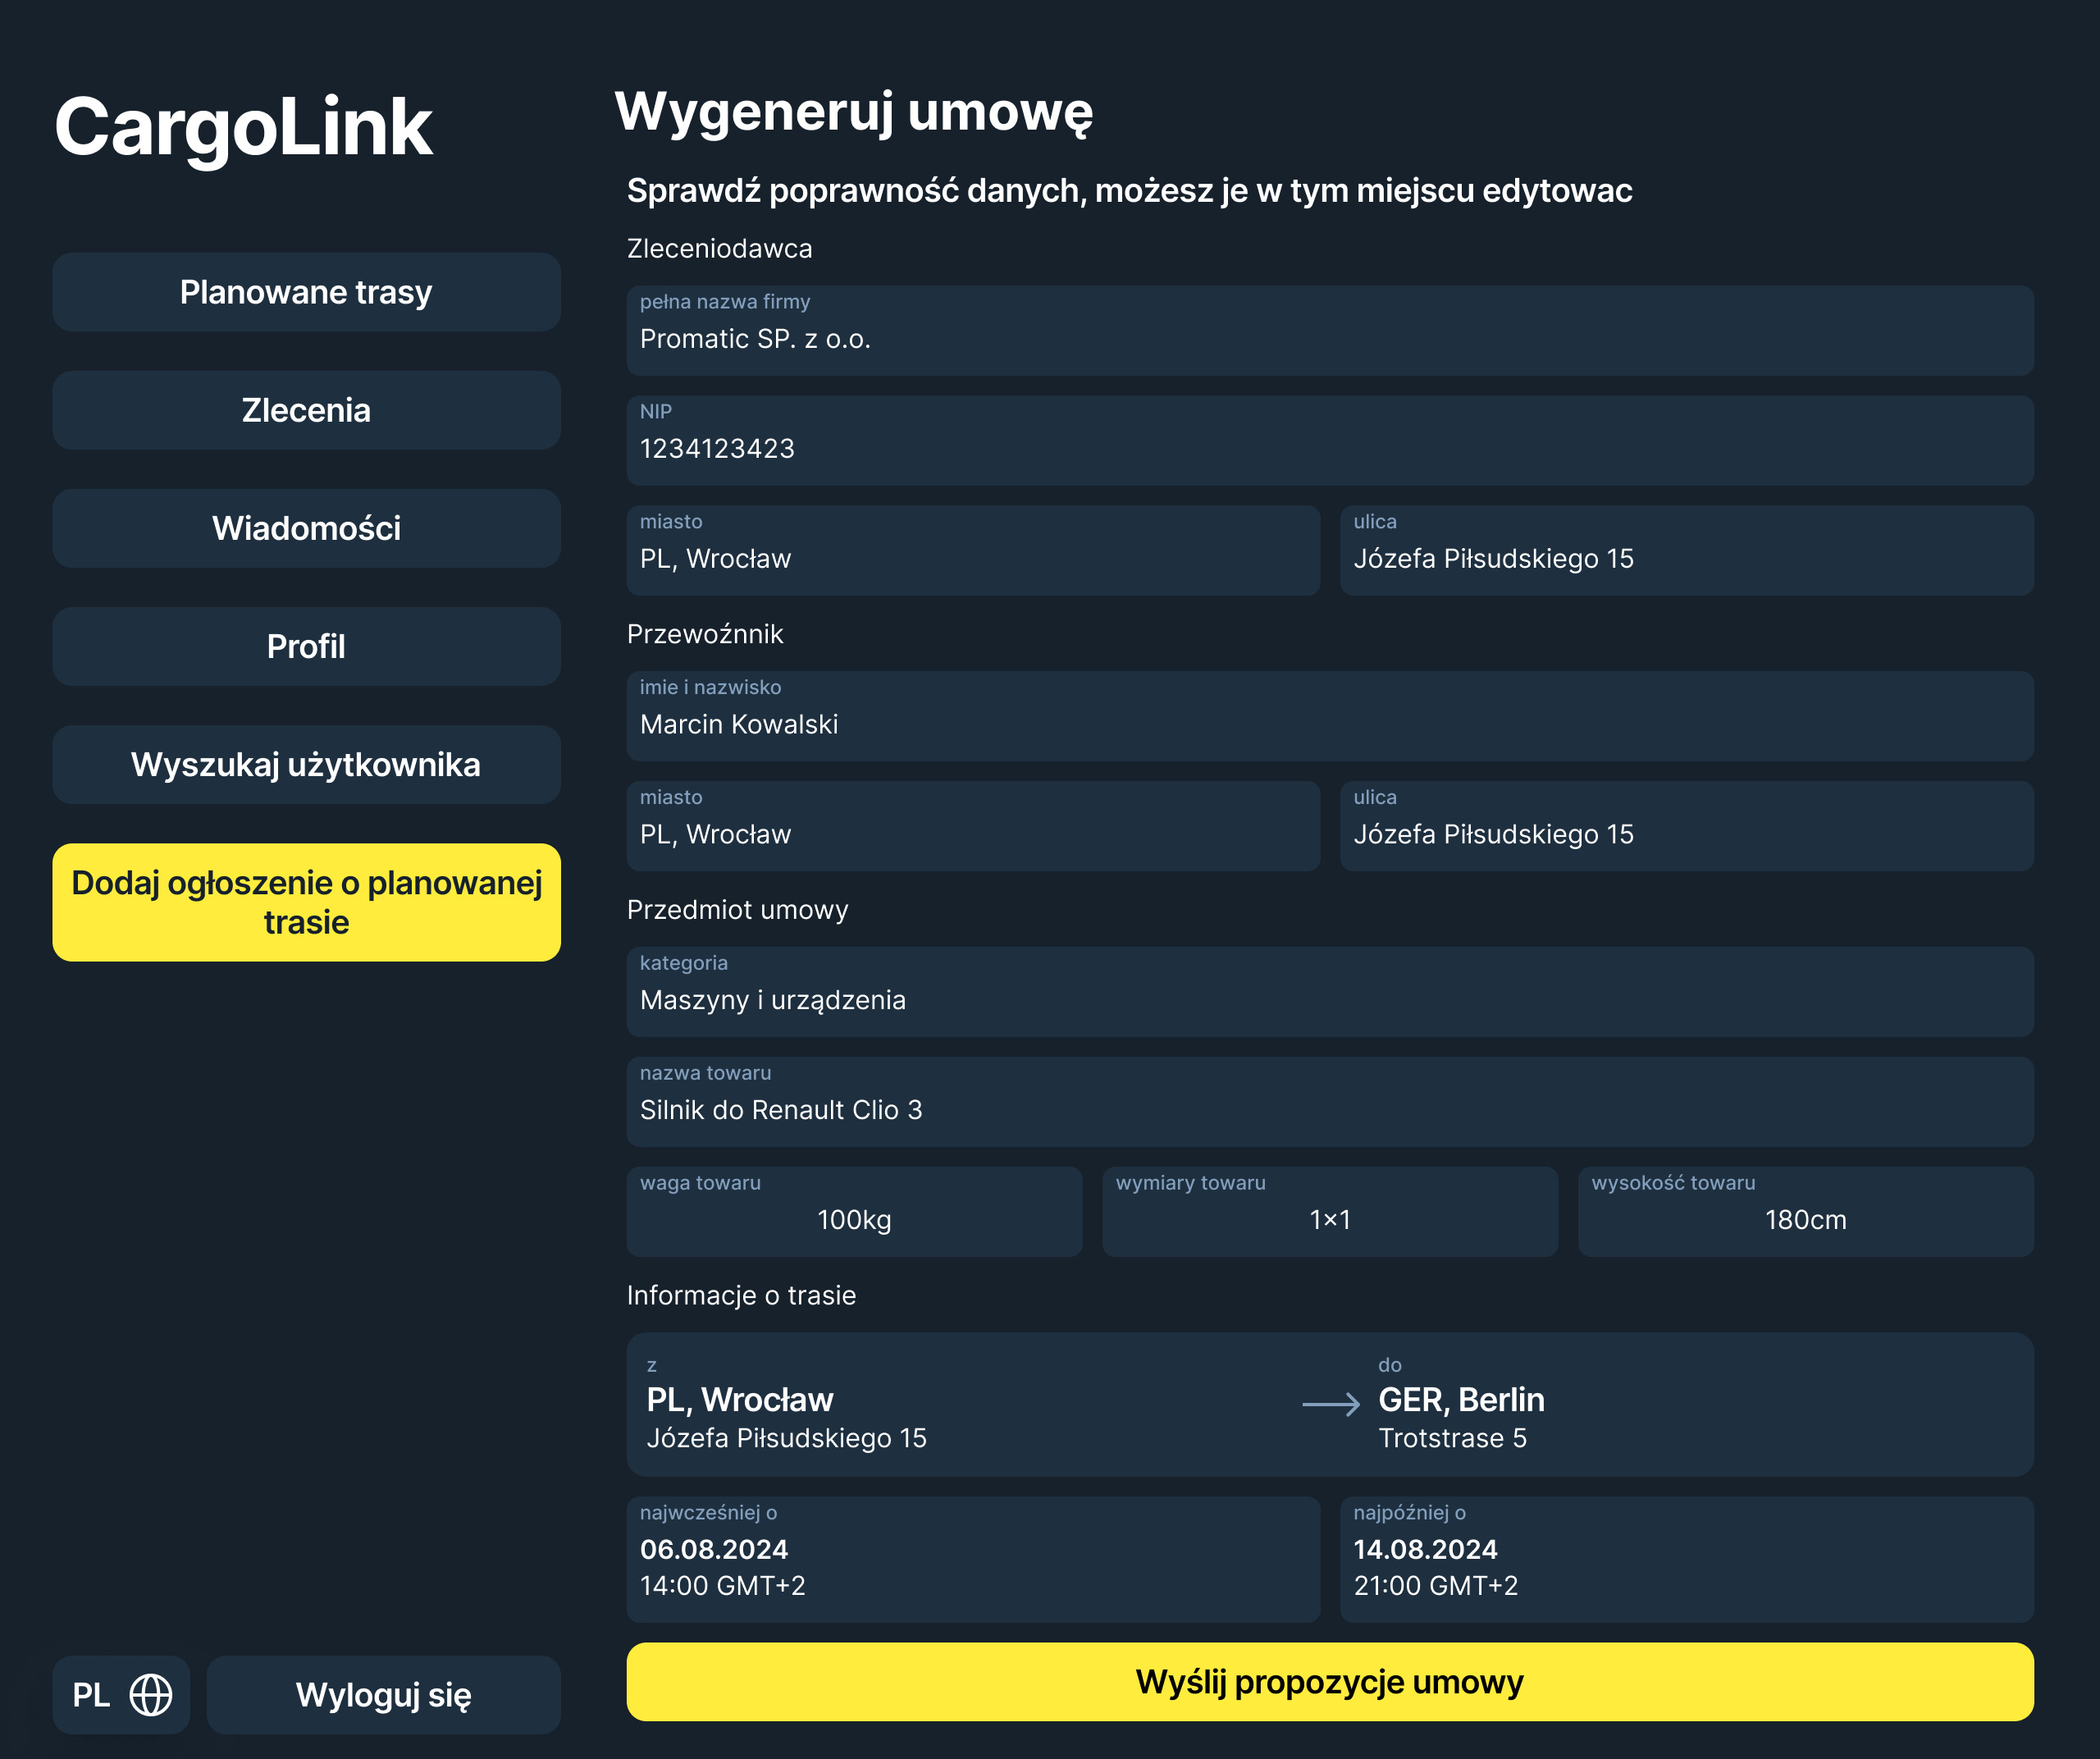
\includegraphics[width=0.7\linewidth]{rozdzial1/wygeneruj_umowe_d.jpg}
	\caption{Formularz generujący umowę w wersji desktopowej}
	\label{Rys. fig:Wygeneruj umowe - desktop}
\end{figure}

\texttt{Zaakceptowanie warunków umowy} \\
Zdarzenie inicjujące: Kliknięcie przycisku \texttt{Otwórz propozycje umowy} \\
Warunki początkowe: Bycie zalogowanym, rozmówca musi wysłać propozycje umowy \\
Przebieg podstawowy realizacji przypadku użycia: \\
\begin{enumerate}
    \item kliknięcie przycisku \texttt{Otwórz propozycje umowy} (Rys. \ref{Rys. fig:Czat - mobile}.b lub \ref{Rys. fig:Czat - desktop});
    \item kliknięcie przycisku \texttt{Akceptuje warunki} (Rys. \ref{Rys. fig:Potwierdz umowe - mobile} lub \ref{Rys. fig:Potwierdz umowe - desktop}).
\end{enumerate}
Warunki końcowe: System generuje gotowy do podpisania dokument w formacie PDF. \\
\begin{figure}[H]
	\centering
		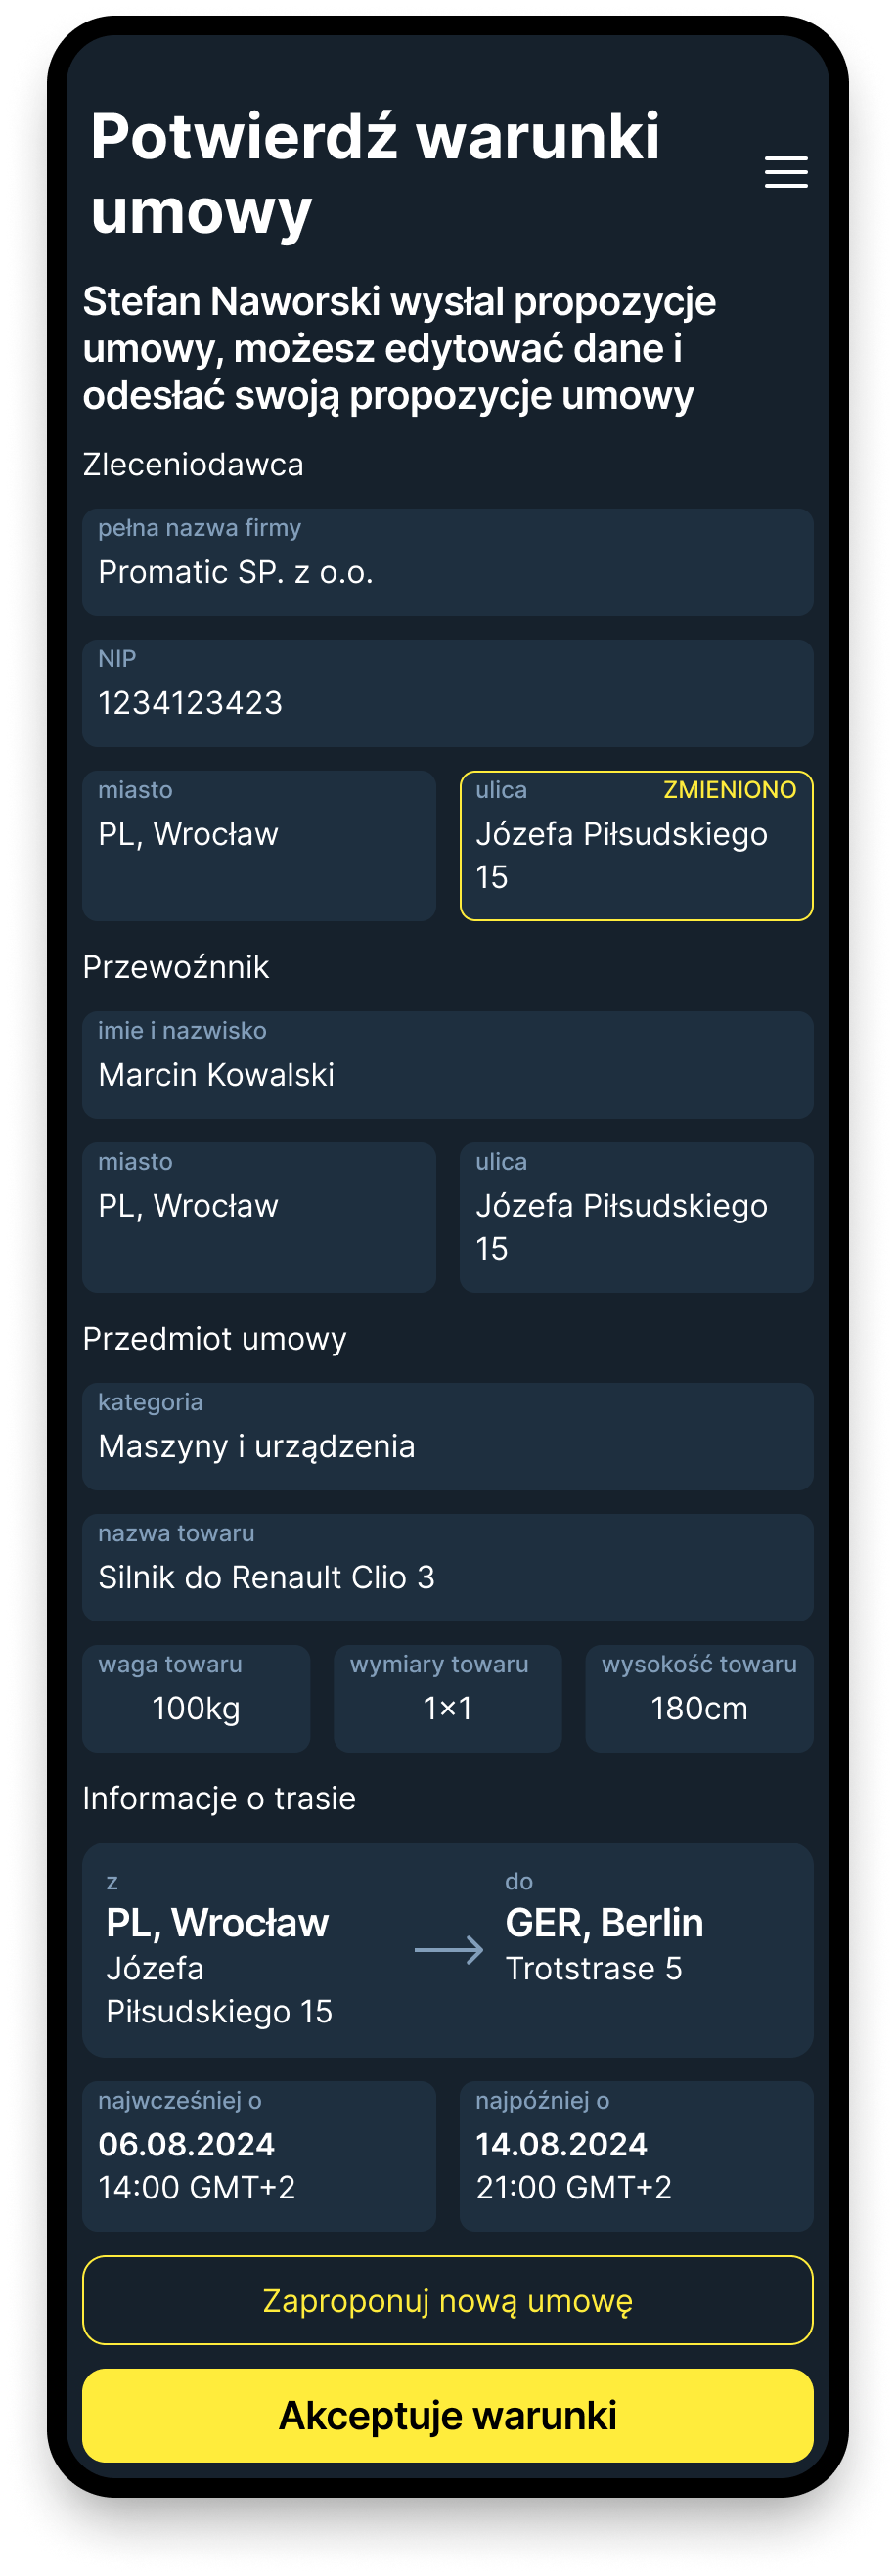
\includegraphics[width=0.3\linewidth]{rozdzial1/potwierdz_umowe_m.png}
	\caption{Zaakceptowanie warunków umowy w wersji mobilnej}
	\label{Rys. fig:Potwierdz umowe - mobile}
\end{figure}
\begin{figure}[H]
	\centering
		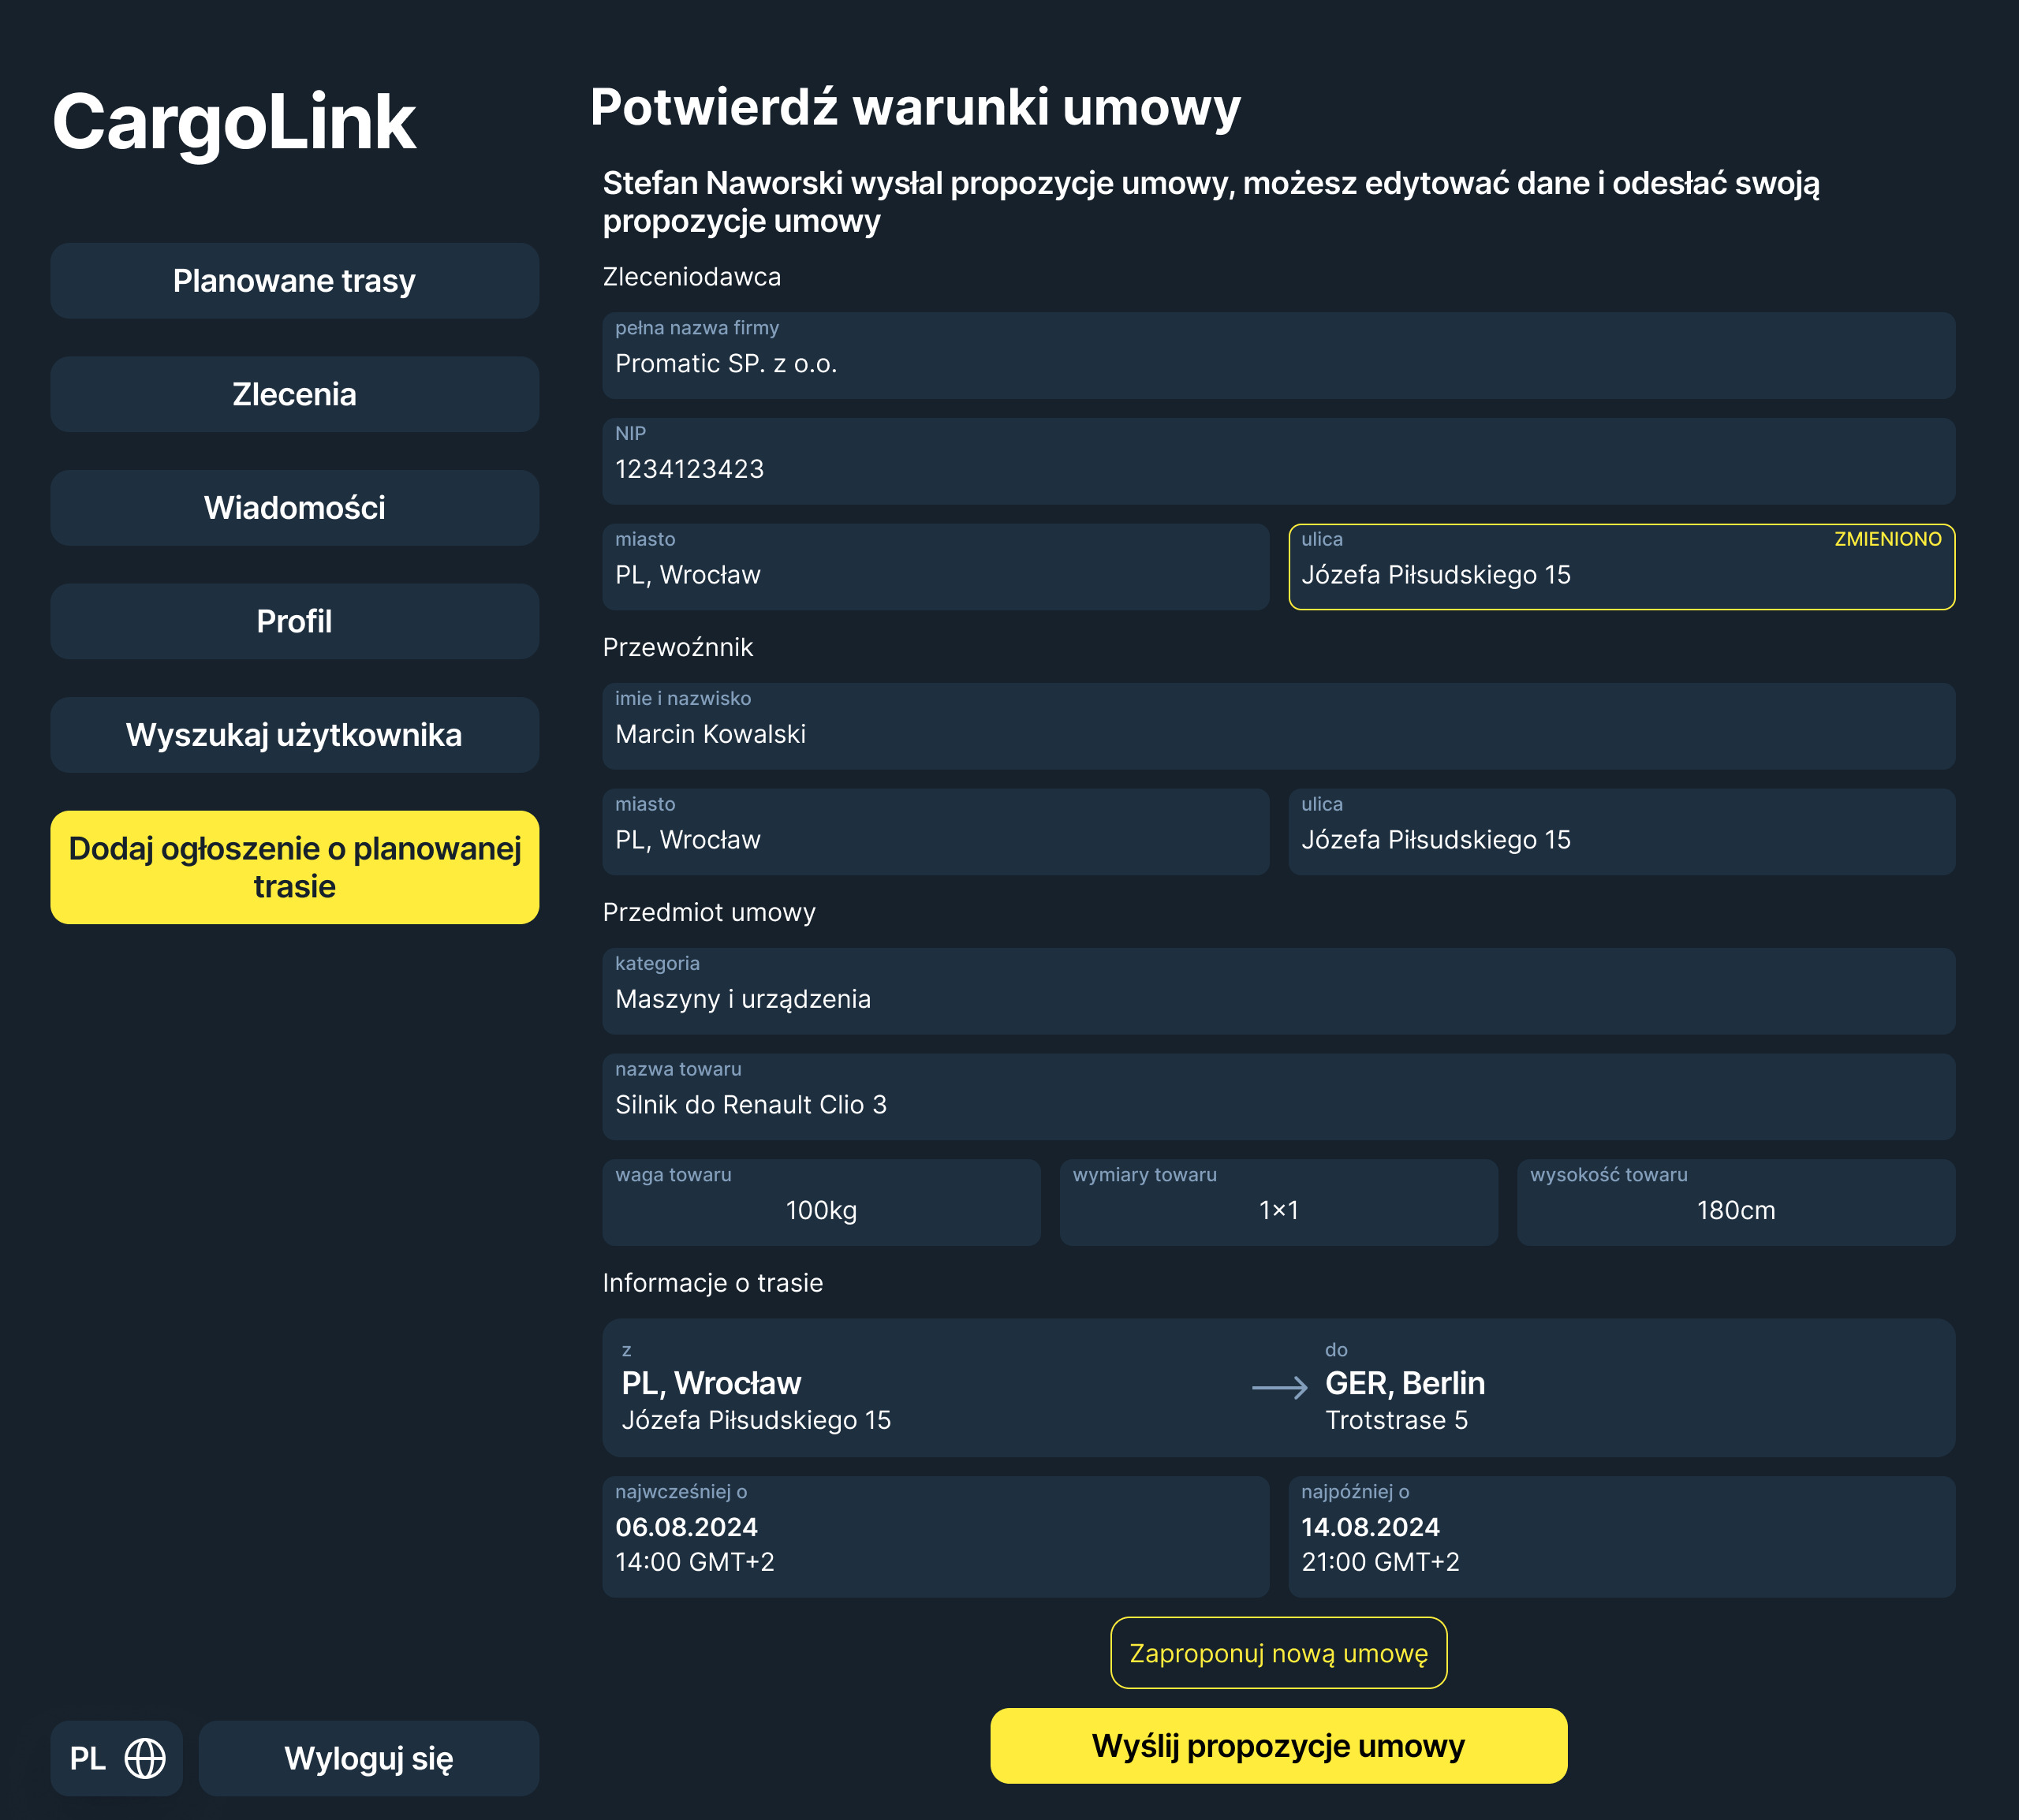
\includegraphics[width=0.7\linewidth]{rozdzial1/potwierdz_umowe_d.jpg}
	\caption{Zaakceptowanie warunków umowy w wersji mobilnej}
	\label{Rys. fig:Potwierdz umowe - desktop}
\end{figure}

\texttt{Modyfikacja warunków umowy} \\
Zdarzenie inicjujące: Kliknięcie przycisku \texttt{Otwórz propozycje umowy} \\
Warunki początkowe: Bycie zalogowanym, rozmówca musi wysłać propozycje umowy \\
Przebieg podstawowy realizacji przypadku użycia: \\
\begin{enumerate}
    \item kliknięcie przycisku \texttt{Otwórz propozycje umowy} (Rys. \ref{Rys. fig:Czat - mobile}.b lub \ref{Rys. fig:Czat - desktop});
    \item użytkownik zmienia wartości w formularzu;
    \item kliknięcie przycisku \texttt{Zaproponuj nową umowe} (Rys. \ref{Rys. fig:Potwierdz umowe - mobile} lub \ref{Rys. fig:Potwierdz umowe - desktop}).
\end{enumerate}
Warunki końcowe: Do rozmówcy wysyłana jest nowa wersja umowy wraz z zaznaczonymi wartościami, które uległy zmianie.\\
Przebieg alternatywny w realizacji podpunktu (3a): Wprowadzone dane są niepoprawne, system informuje o niepowodzeniu. \\

\texttt{Wylogowanie} \\
Zdarzenie inicjujące: kliknięcie przycisku \texttt{Wyloguj się} (Rys. \ref{Rys. fig:Dodawanie nowego ogłoszenia o planowanej trasie - ab - mobile}.a lub np. \ref{Rys. fig:Dodawanie nowego ogłoszenia o planowanej trasie - ab - desktop}.a). \\
Warunki początkowe: Użytkownik jest zalogowany. \\
Przebieg podstawowy realizacji przypadku użycia:
\begin{enumerate}
    \item kliknięcie przycisku \texttt{Wyloguj się} (Rys. \ref{Rys. fig:Dodawanie nowego ogłoszenia o planowanej trasie - ab - mobile}.a lub np. \ref{Rys. fig:Dodawanie nowego ogłoszenia o planowanej trasie - ab - desktop}.a).
\end{enumerate}
Warunki końcowe: Wylogowanie użytkownika.\\

\pagebreak
\texttt{Edycja profilu} \\
Zdarzenie inicjujące: Kliknięcie przycisku \texttt{Profil} \\
Warunki początkowe: Bycie zalogowanym \\
Przebieg podstawowy realizacji przypadku użycia: \\
\begin{enumerate}
    \item Zdarzenie inicjujące: Kliknięcie przycisku \texttt{Profil} (Rys. \ref{Rys. fig:Dodawanie nowego ogłoszenia o planowanej trasie - ab - mobile}.a lub np. \ref{Rys. fig:Dodawanie nowego ogłoszenia o planowanej trasie - ab - desktop}.b);
    \item Zmiana danych na profilu (Rys. \ref{Edytuj profil - mobile} lub \ref{Edytuj profil - mobile});
    \item Kliknięcie przycisku \texttt{Zapisz}.
\end{enumerate}
Warunki końcowe: zapisanie w bazie danych zmienionych danych. \\
\begin{figure}[H]
	\centering
		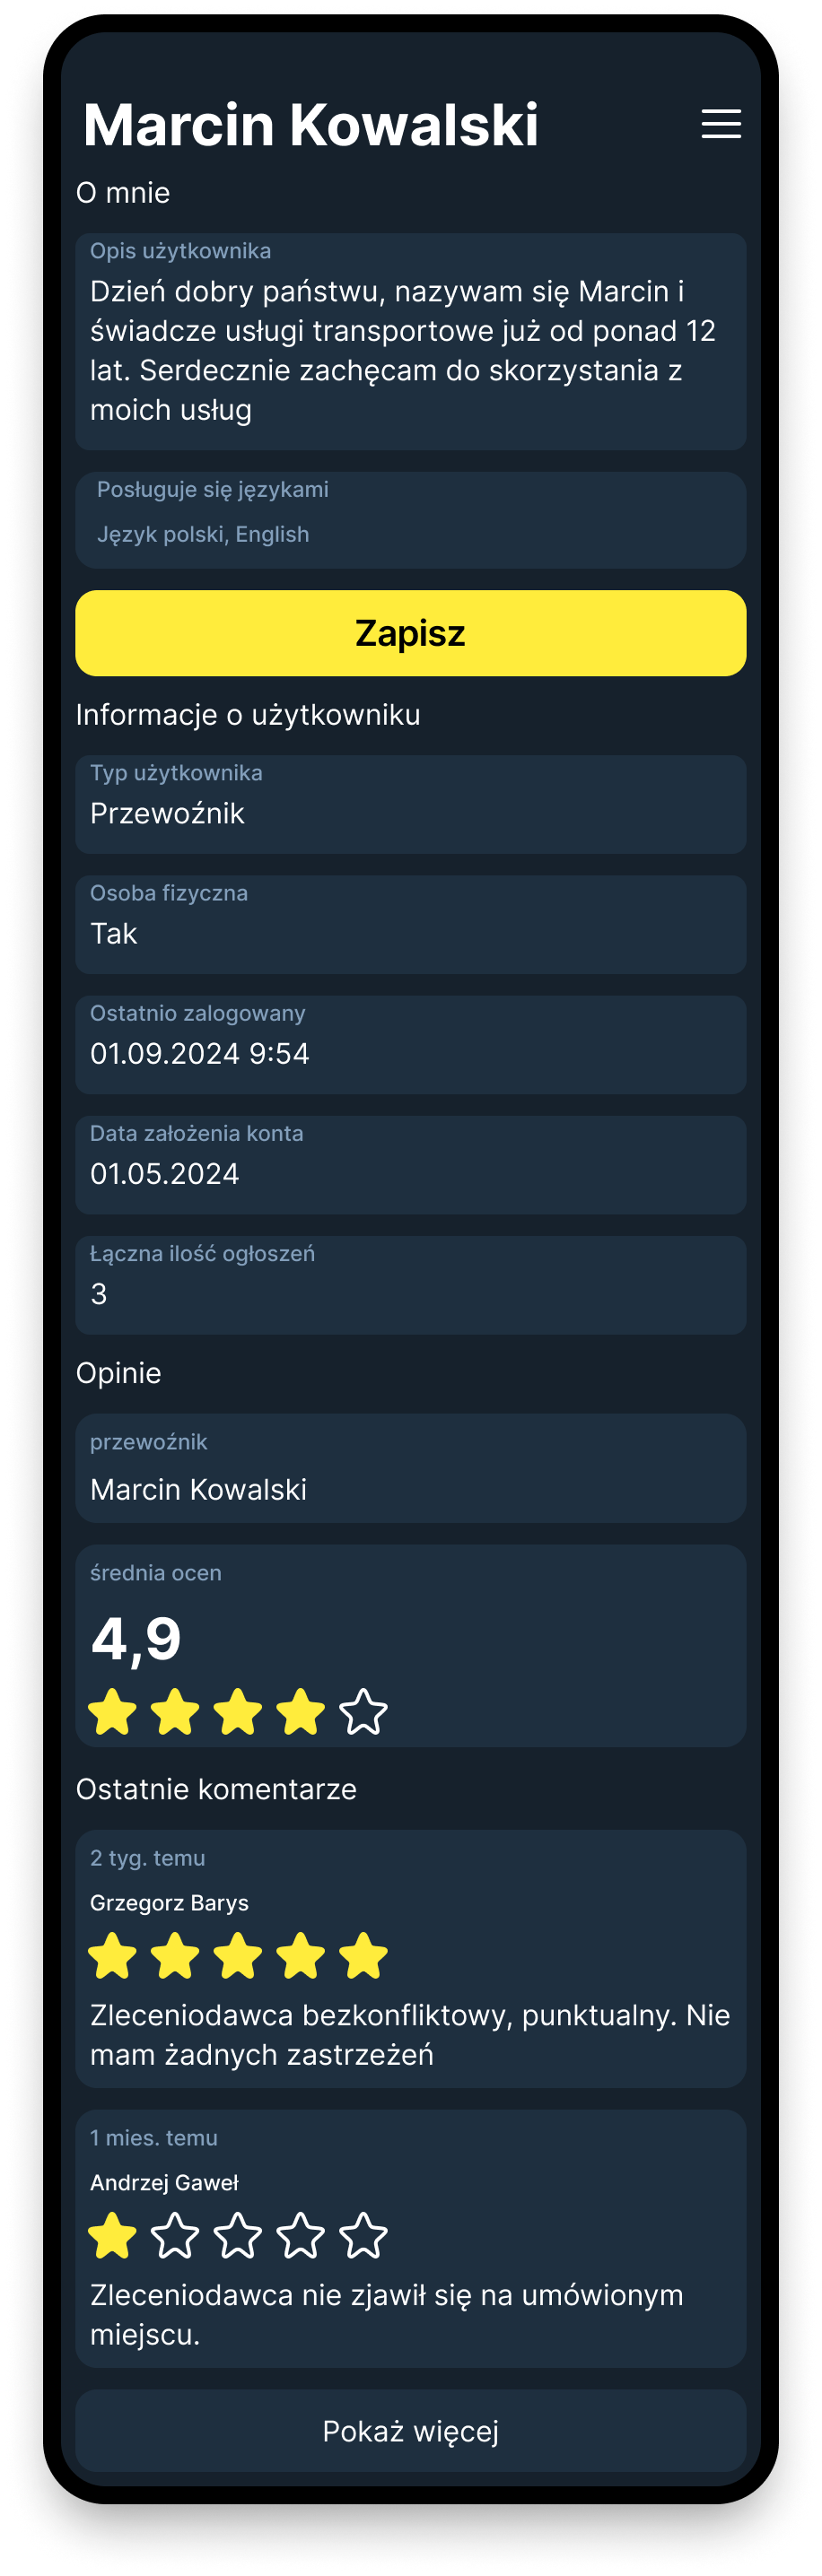
\includegraphics[width=0.3\linewidth]{rozdzial1/edytuj_profil_m.png}
	\caption{Edycja profilu w wersji mobilnej}
	\label{Edytuj profil - mobile}
\end{figure}
\begin{figure}[H]
	\centering
		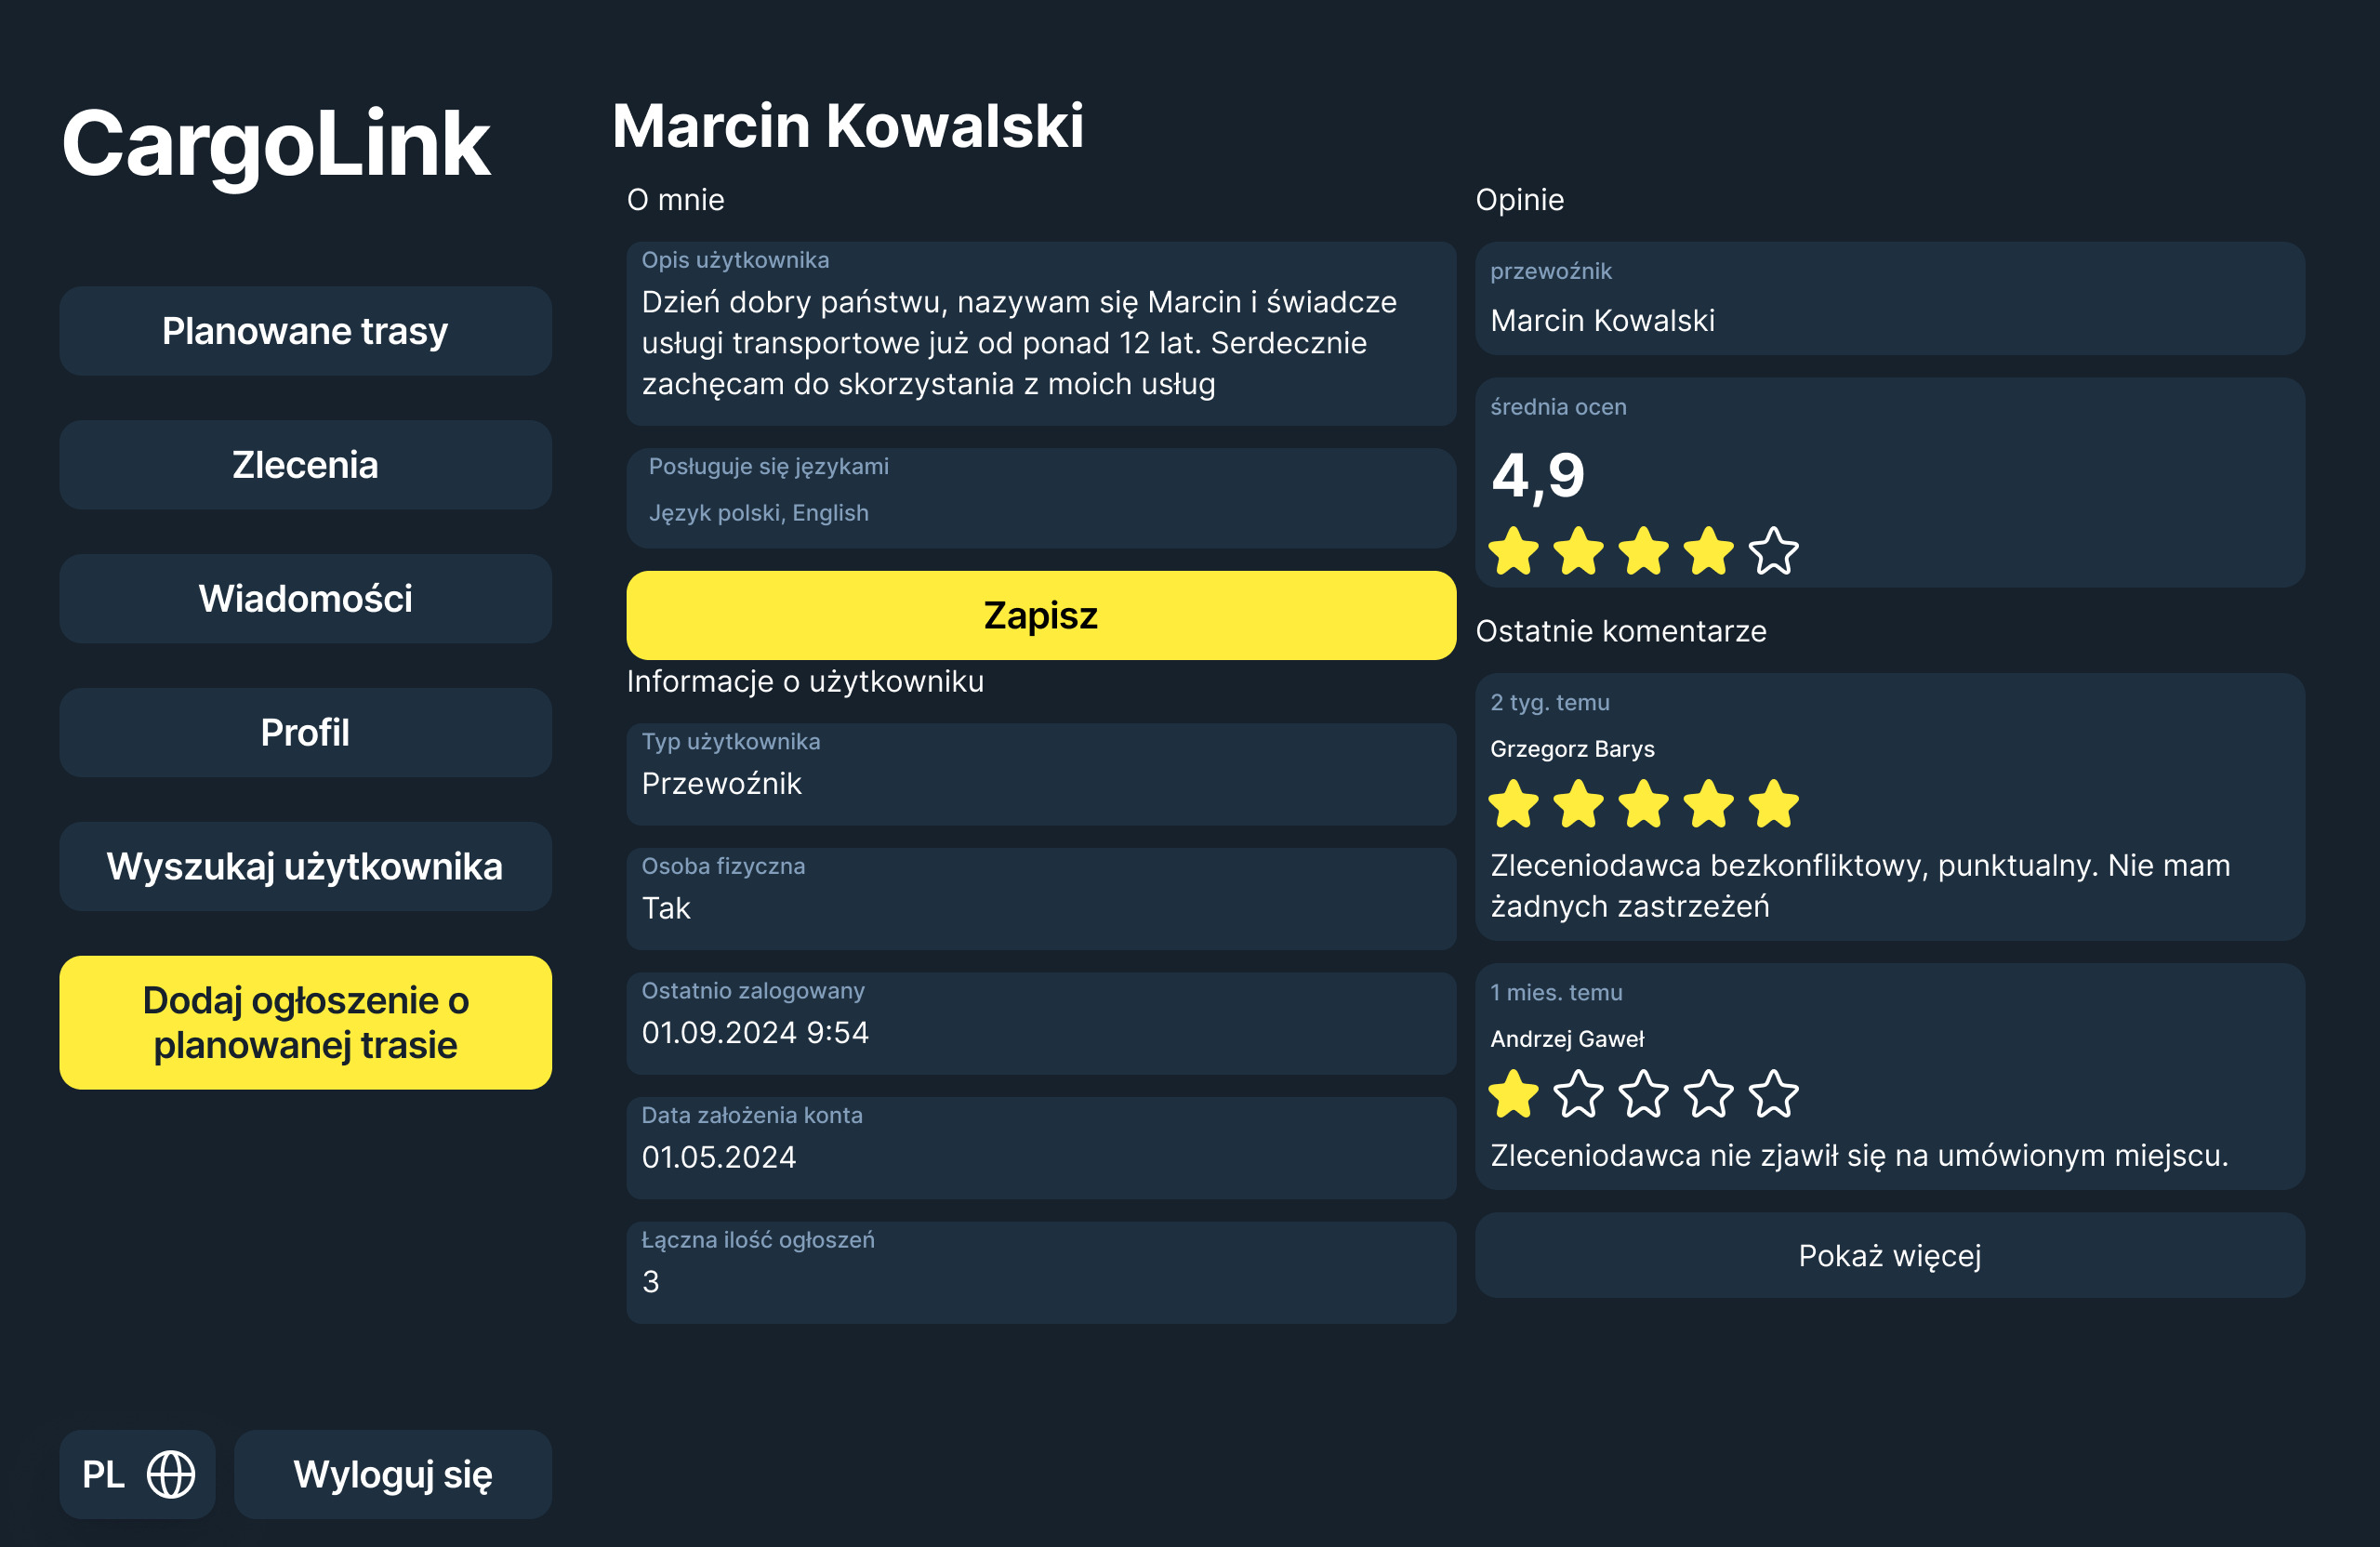
\includegraphics[width=0.7\linewidth]{rozdzial1/edytuj_profil_d.jpg}
	\caption{Edycja profilu w wersji mobilnej}
	\label{Edytuj profil - desktop}
\end{figure}

\texttt{Dodanie opinii o użytkowniku} \\
Zdarzenie inicjujące: Wykonanie przypadku użycia \ref{Wyświetlenie profilu użytkownika} \\
Warunki początkowe: Od wygenerowania umowy między użytkownikami musi minąć 7 dni. \\
Przebieg podstawowy realizacji przypadku użycia: \\
\begin{enumerate}
   \item Wykonanie przypadku użycia \ref{Wyświetlenie profilu użytkownika};
   \item Gdy dodanie opinii będzie możliwe, pojawi się nowy przycisk \texttt{Dodaj opinie} (Rys. \ref{Dodawanie opini - mobile - ab}.a lub \ref{Dodawanie opini - destkop - ab}.a);
   \item Wypełnienie formularza dodawania opinii (Rys. \ref{Dodawanie opini - mobile - ab}.b lub \ref{Dodawanie opini - destkop - ab}.b);
   \item Dodanie opinii o użytkowniku.
\end{enumerate}
Warunki końcowe: Dodanie opinii o użytkowniku \\
\begin{figure}[H]
	\centering
	\begin{tabular}{@{}ccc@{}}
            a) & b)\\
    \vtop{\null\hbox{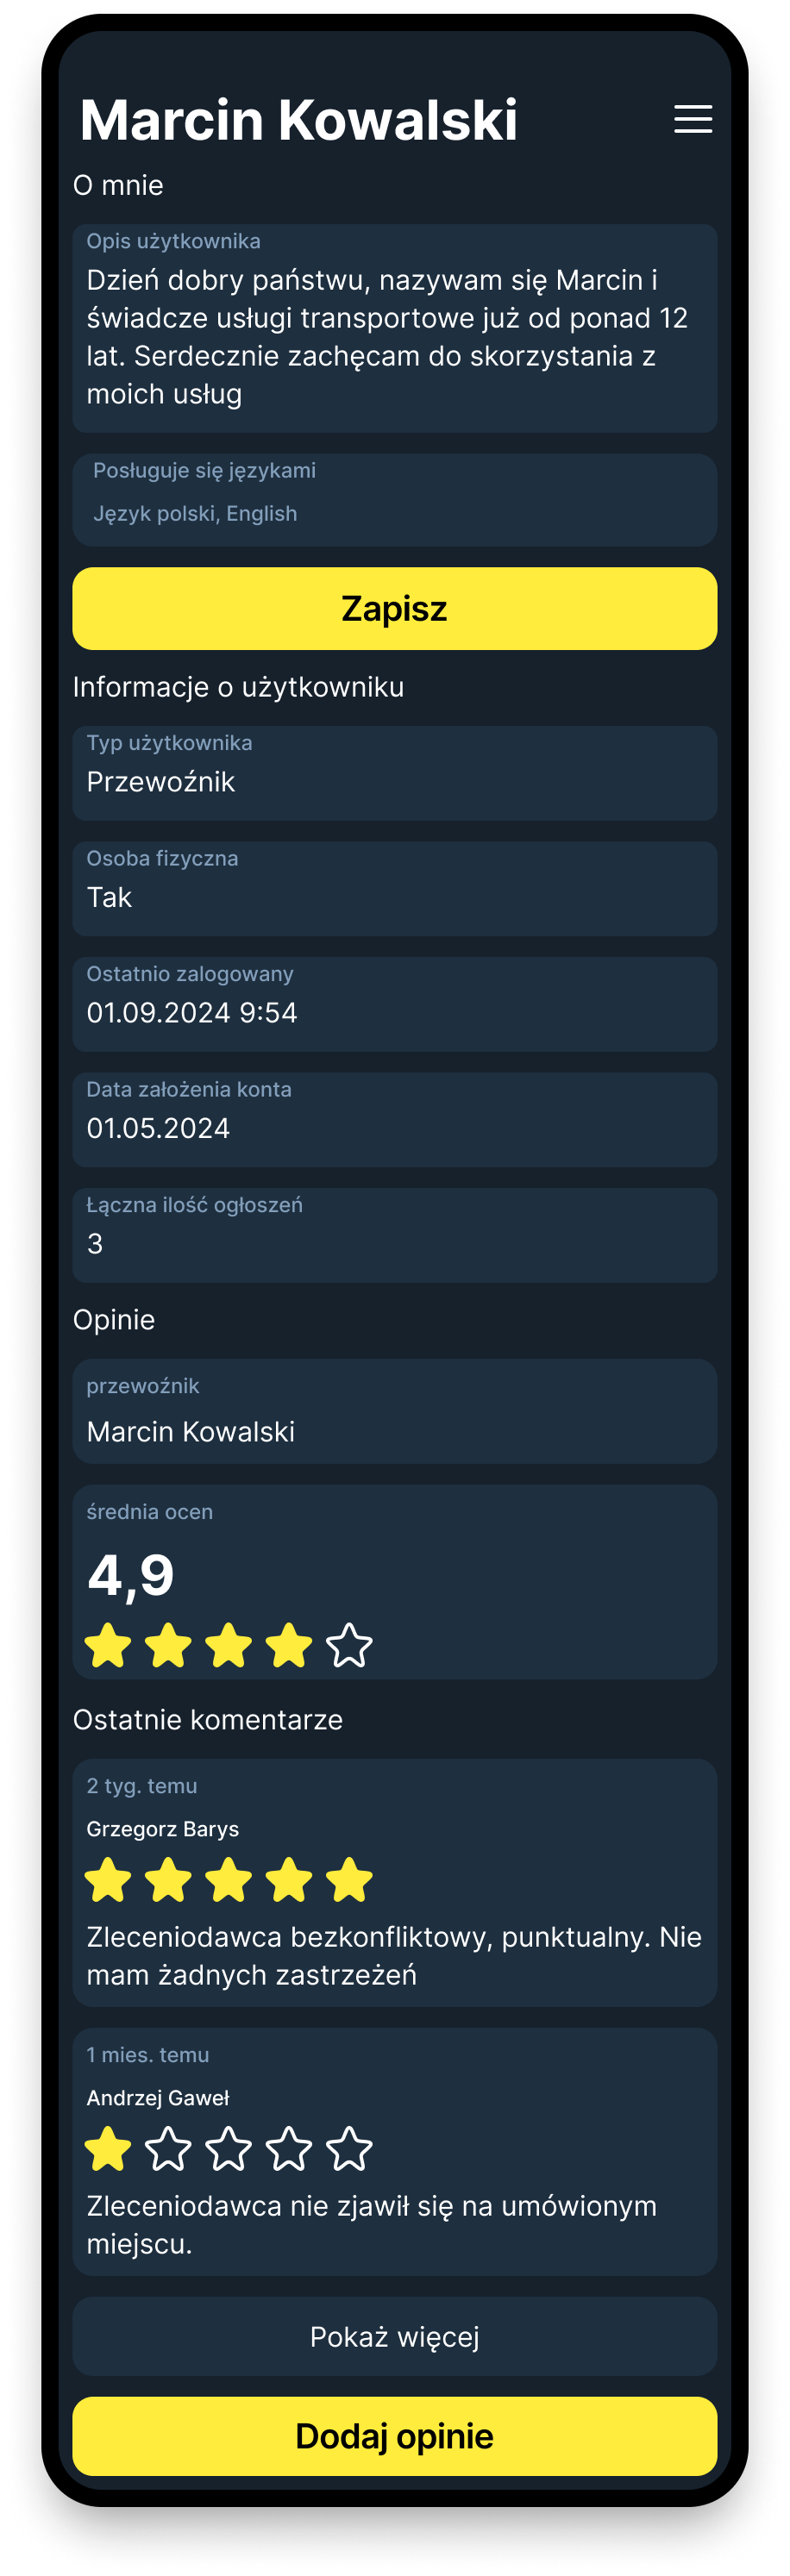
\includegraphics[width=0.3\linewidth]{rozdzial1/profil_opinia_m.png}}} &
    \vtop{\null\hbox{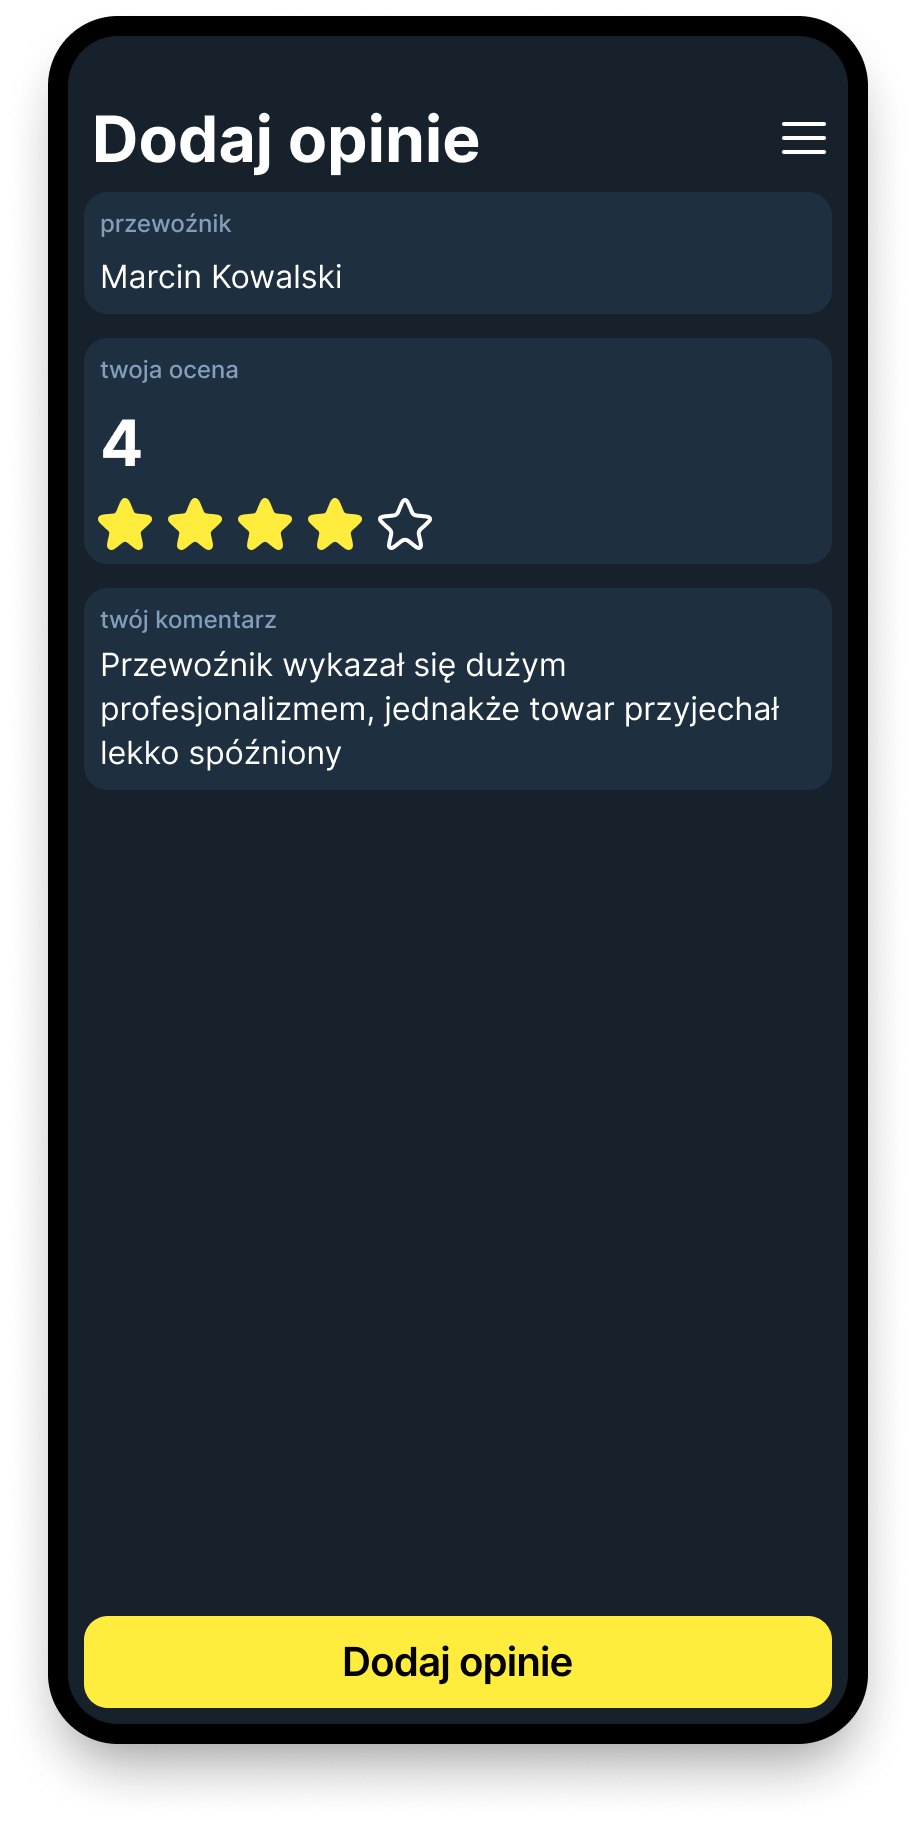
\includegraphics[width=0.3\linewidth]{rozdzial1/dodaj_opinie_m.png}}}
    \end{tabular}
    \caption{Dodawanie opinii o użytkowniku w wersji mobilnej: a) Profil użytkownika gdy dostępne jest dodanie opinii b) Formularz dodawania opinii}
	\label{Dodawanie opini - mobile - ab}
\end{figure}
\begin{figure}[H]
 \centering
  \begin{tabular}{@{}ccc@{}}
  a) & b)\\
  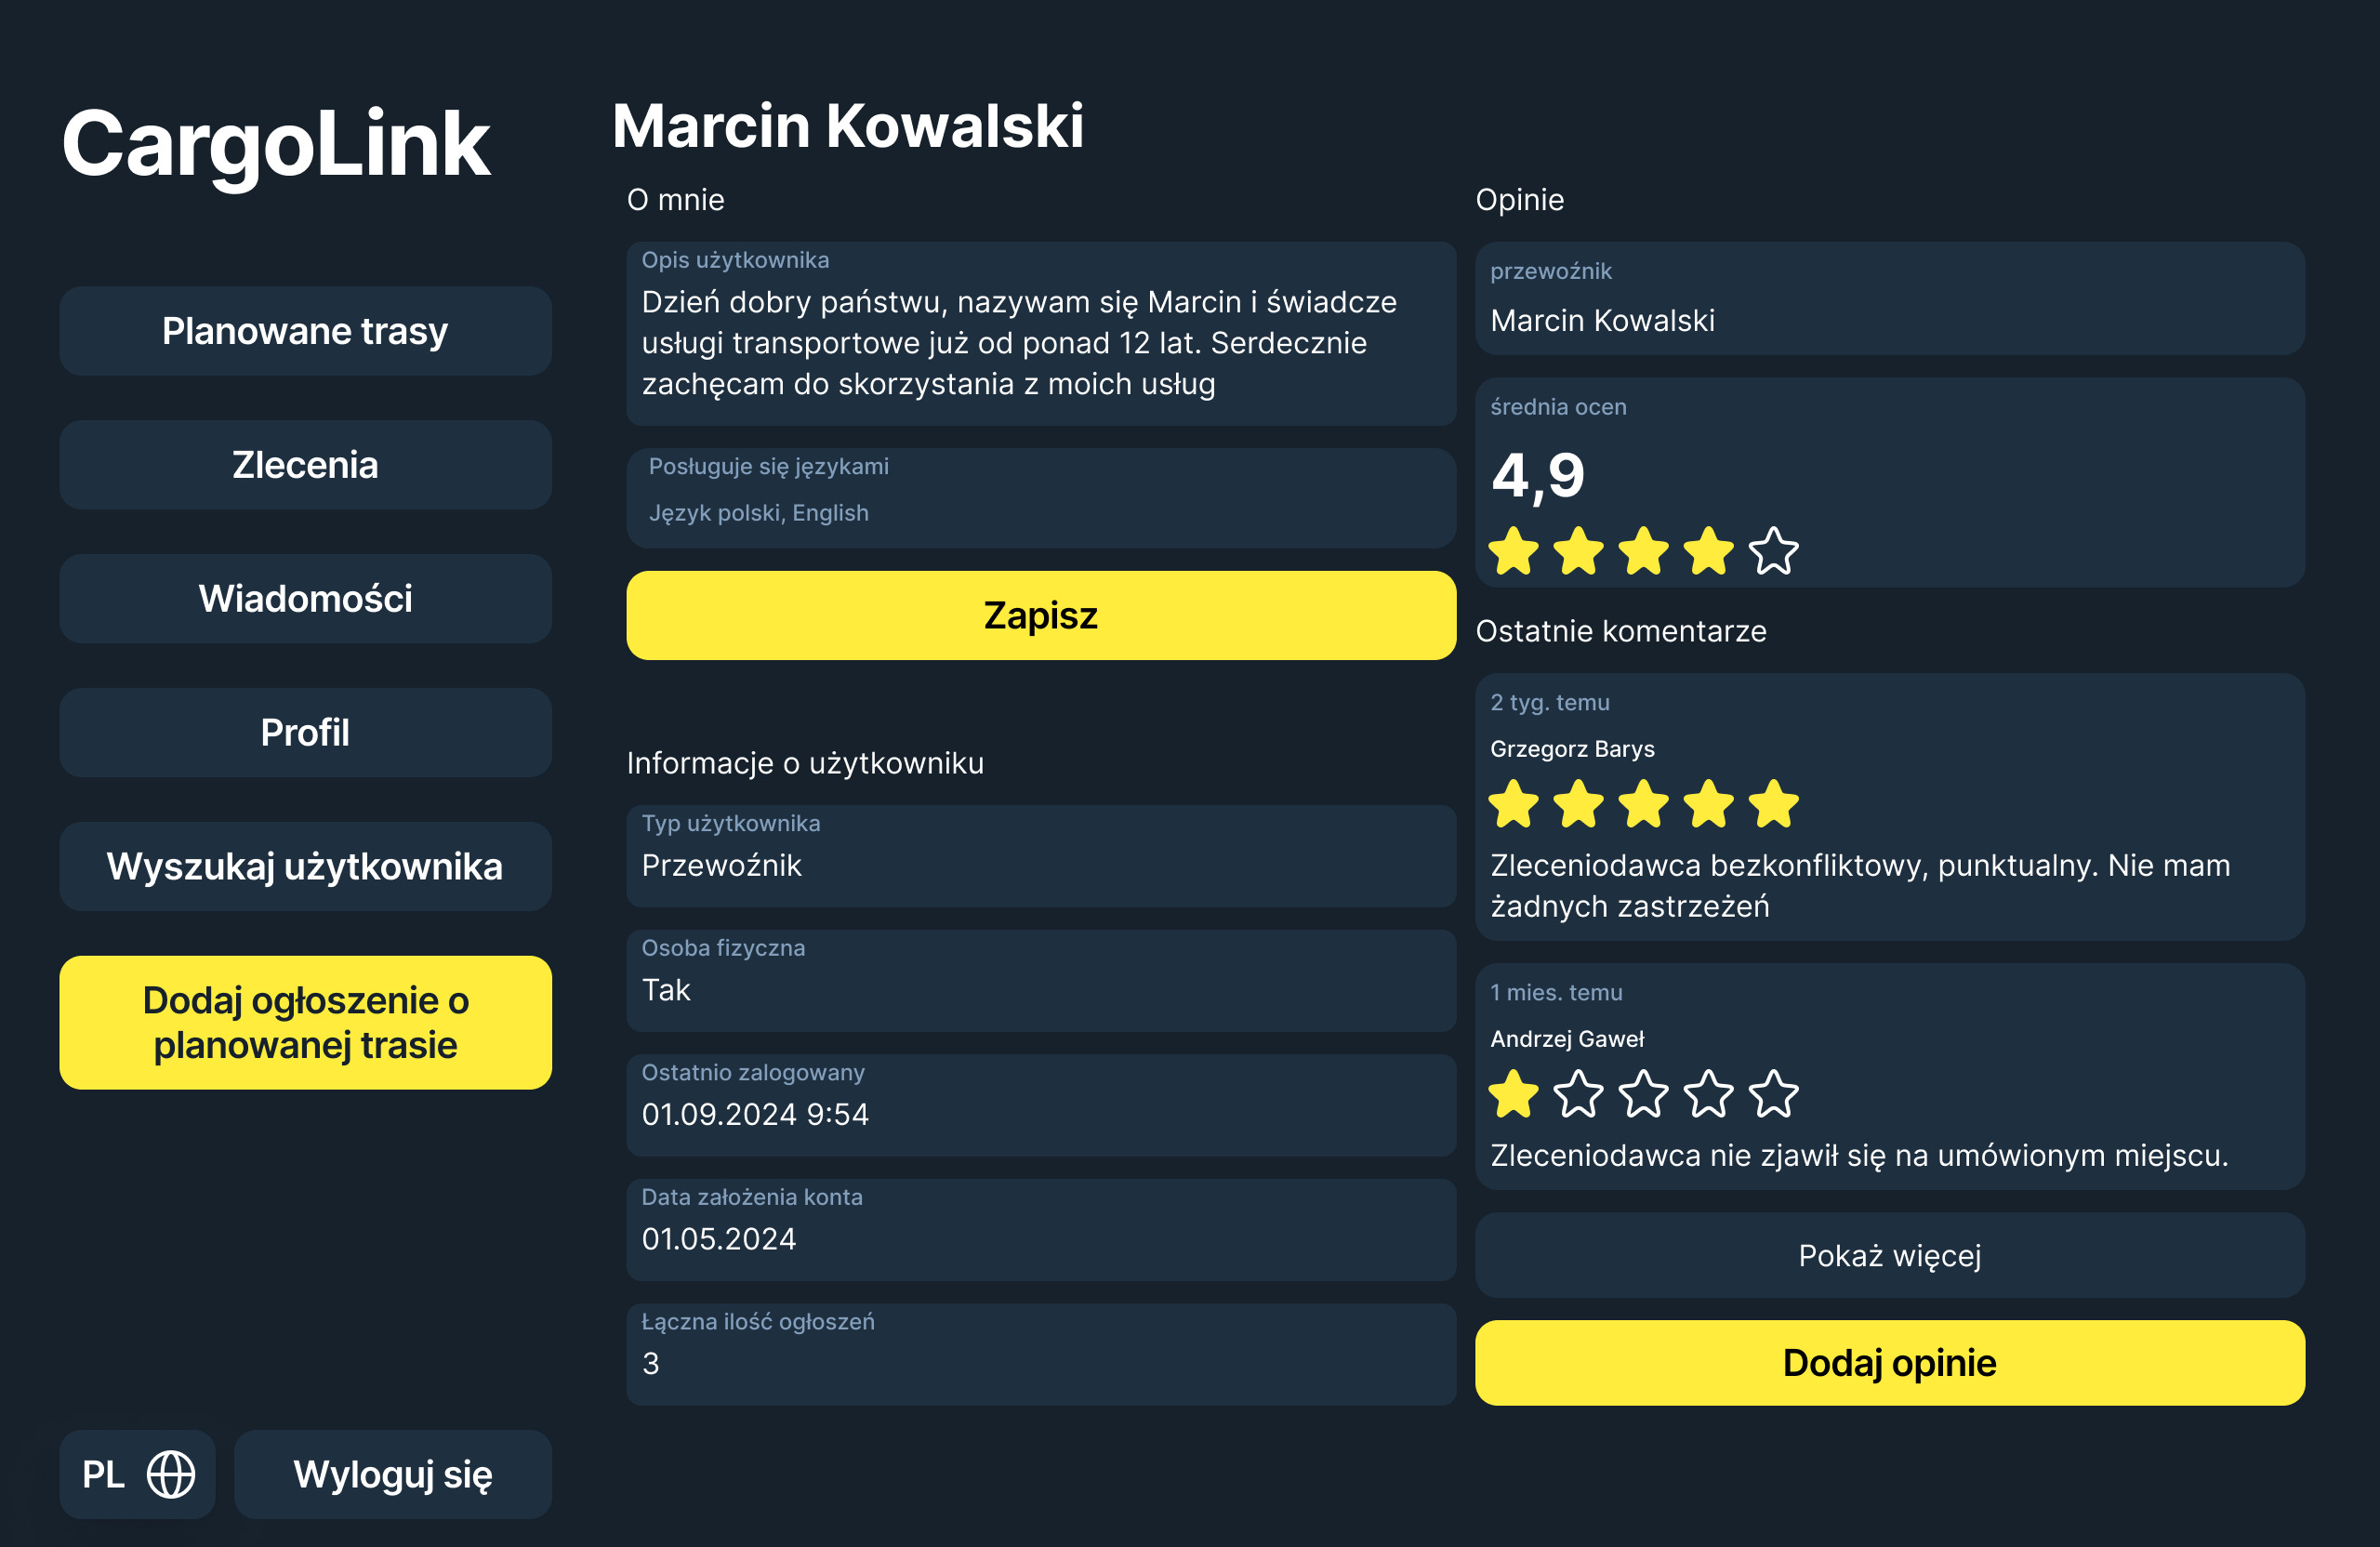
\includegraphics[width=0.45\textwidth]{rozdzial1/profil_opinia_d.jpg} &
  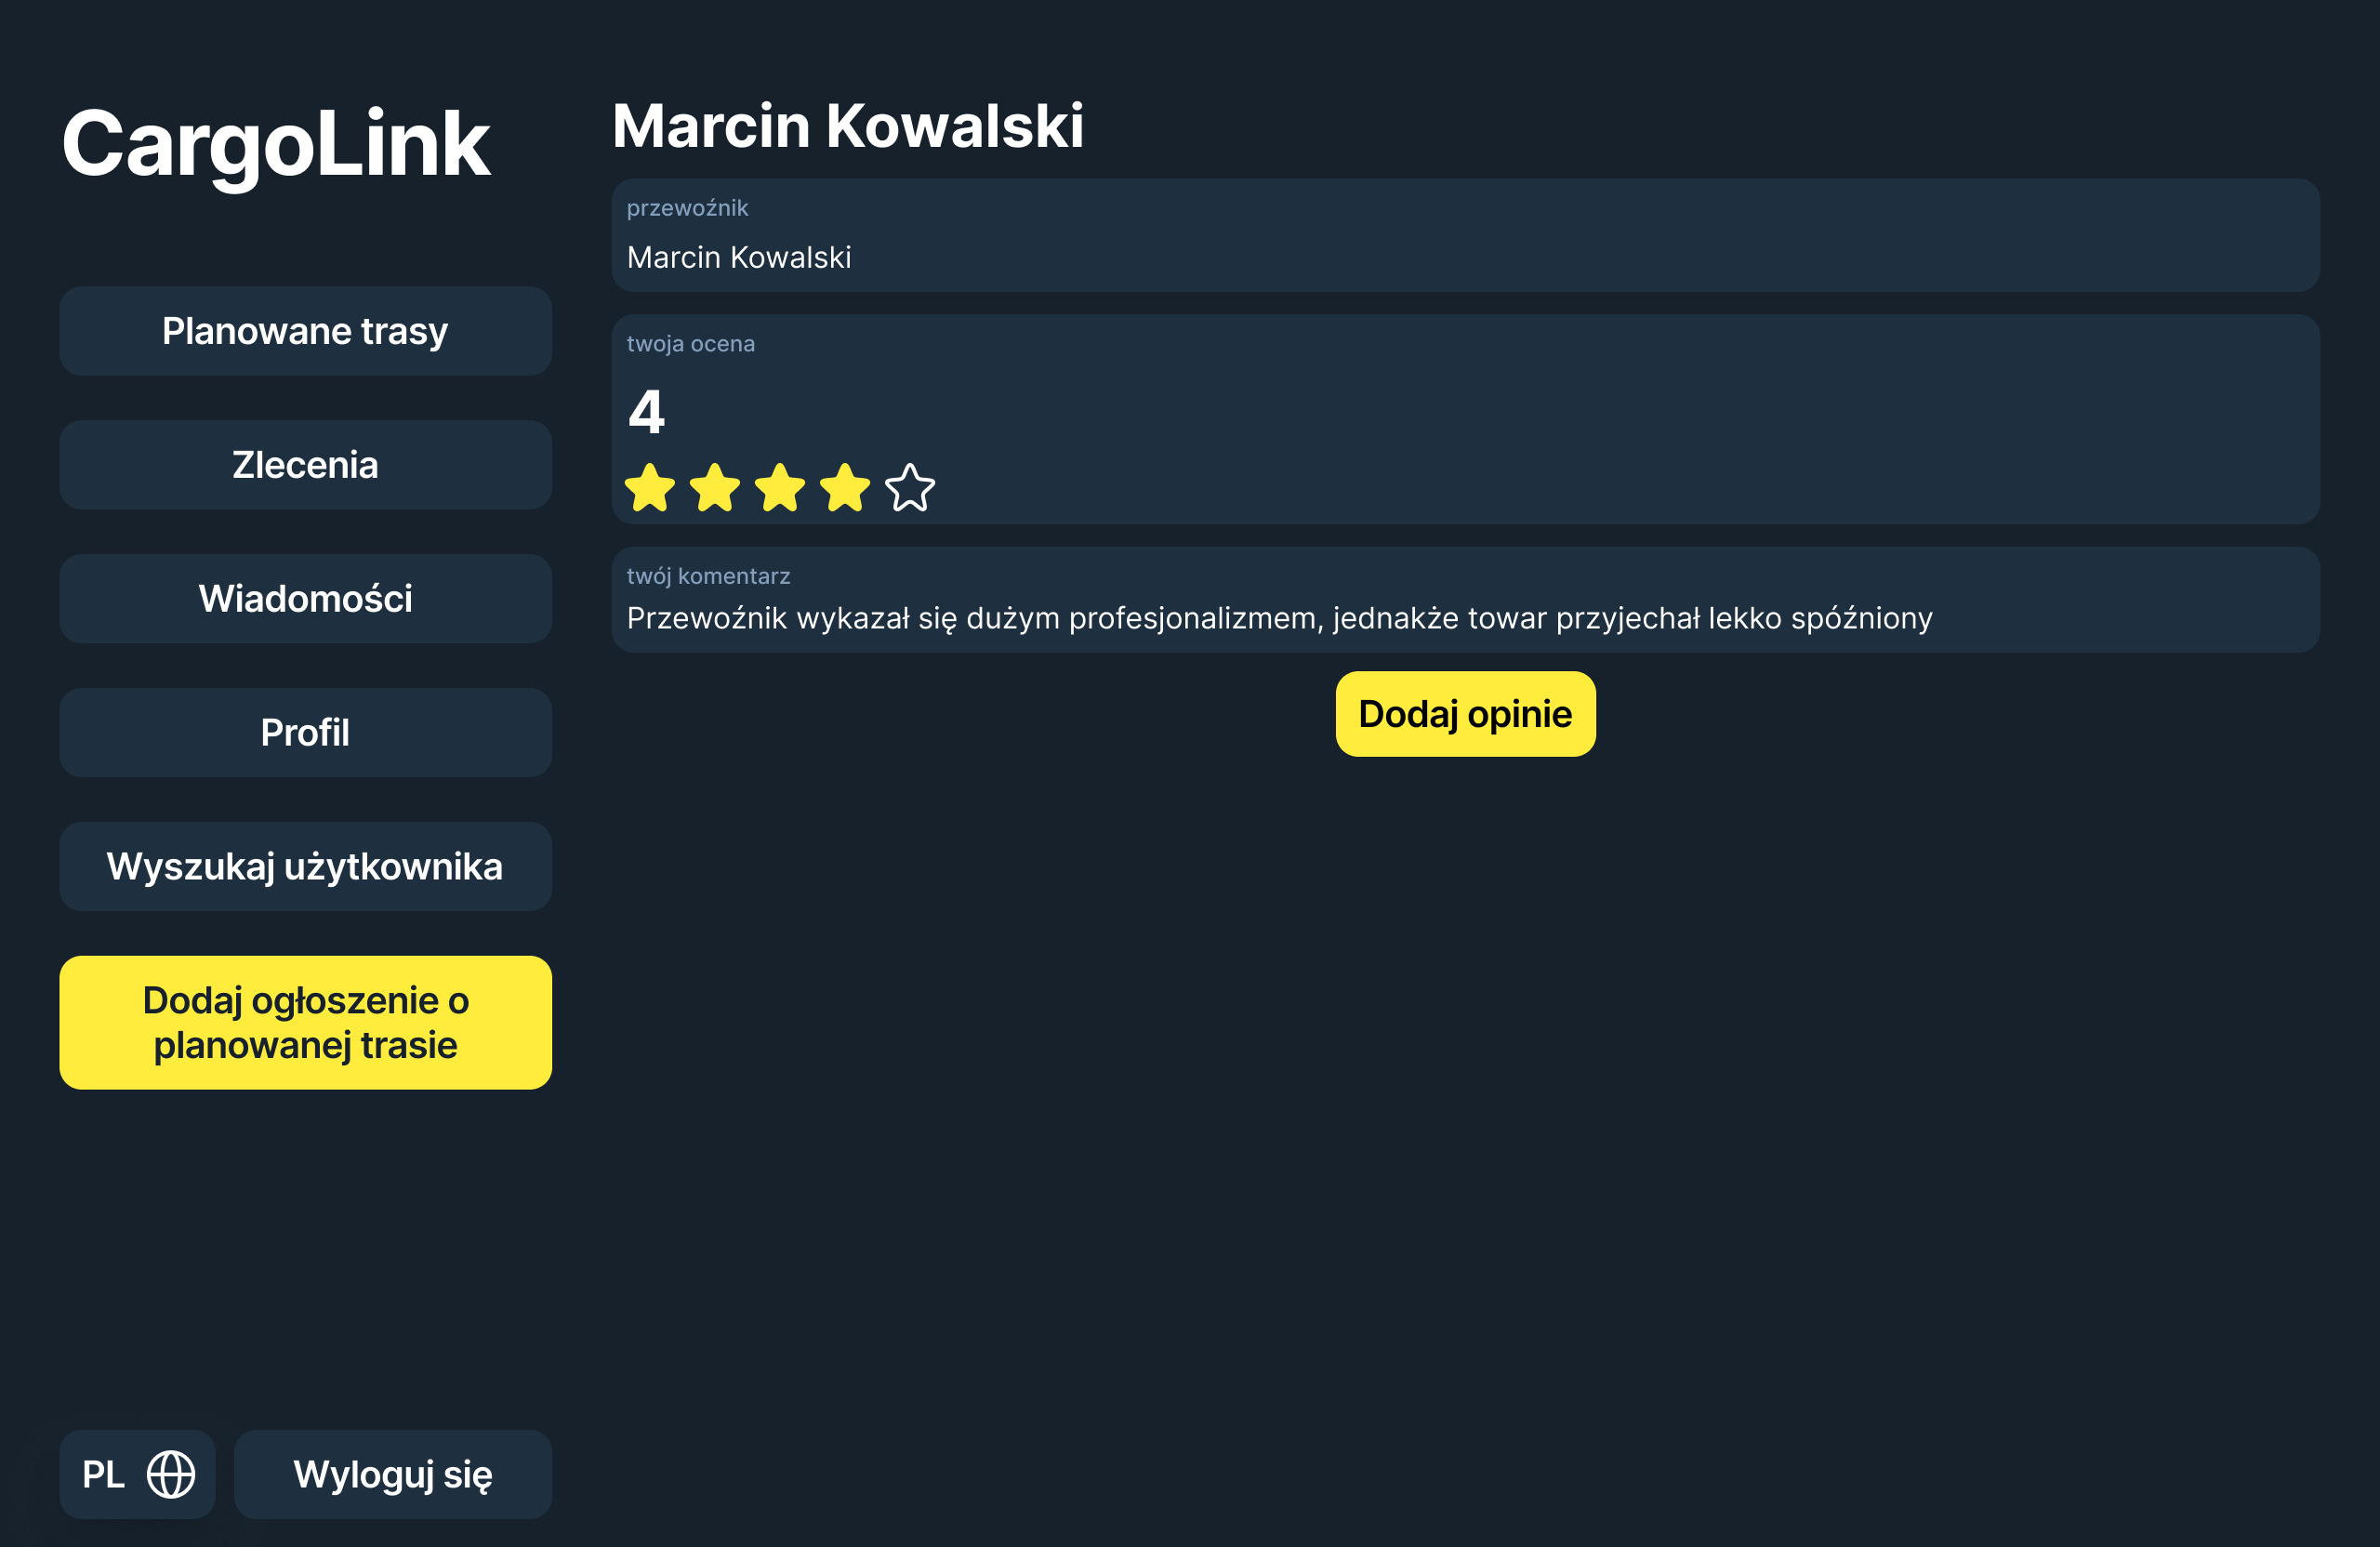
\includegraphics[width=0.45\textwidth]{rozdzial1/dodaj_opinie_d.jpg}
  \end{tabular}
 \caption{Dodawanie opinii o użytkowniku w wersji desktopowej: a) Profil użytkownika gdy dostępne jest dodanie opinii b) Formularz dodawania opinii}
 \label{Dodawanie opini - destkop - ab}
\end{figure}

\subsection{Zleceniodawca}
\begin{figure}[H]
	\centering
		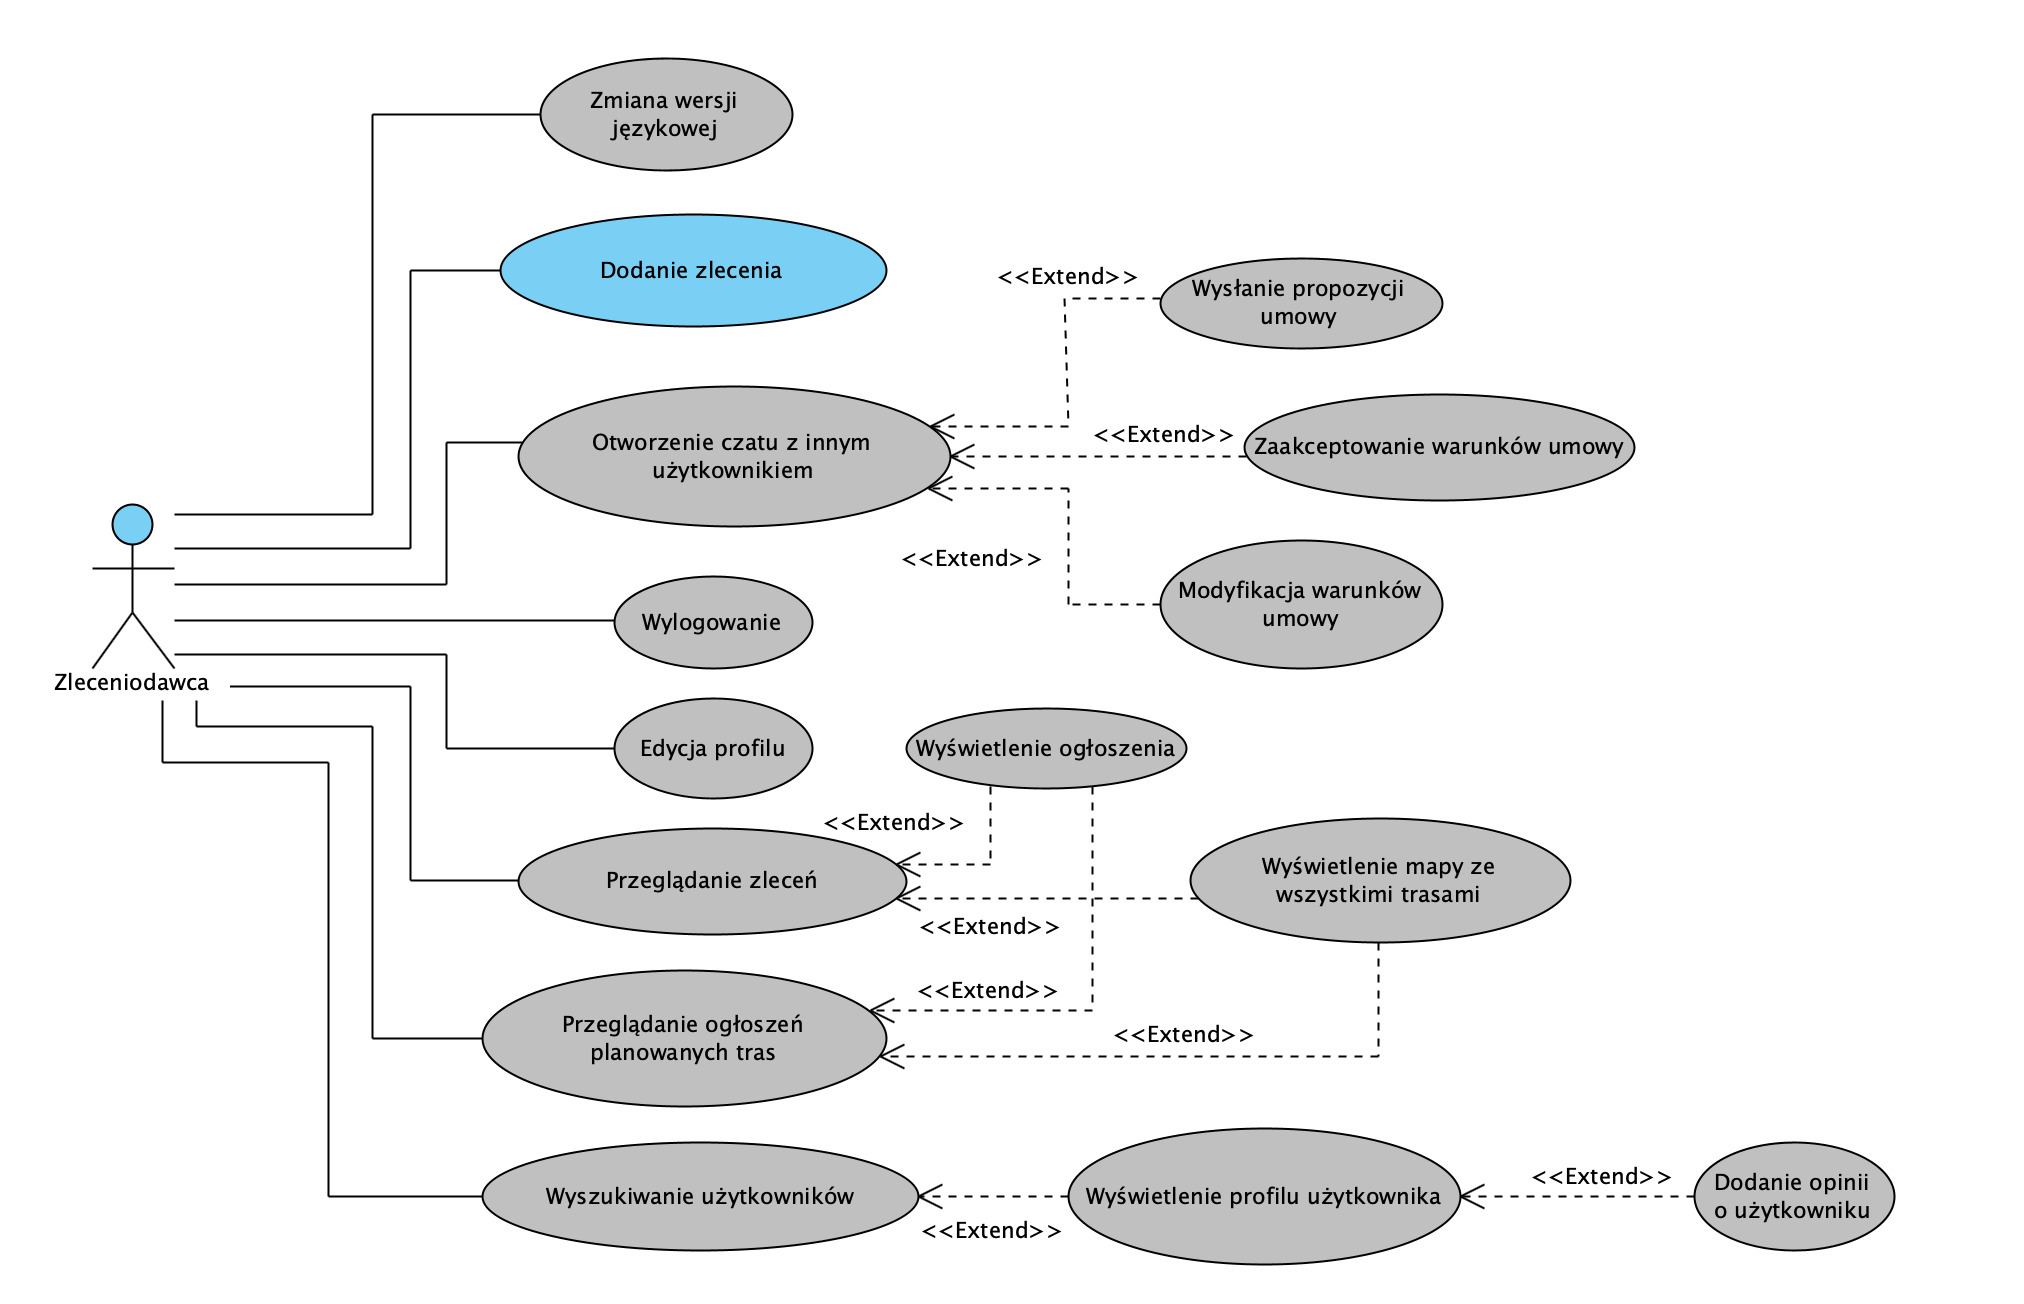
\includegraphics[width=\linewidth]{rozdzial1/PU_zleceniodawca.jpg}
	\caption{Diagram przedstawiający przypadki użycia aktora \texttt{Zleceniodawca}}
	\label{Rys. fig:Diagram przedstawiający przypadki użycia aktora Zleceniodawca}
\end{figure}
Na powyższym diagramie przedstawione zostały przypadki użycia dla \texttt{Zleceniodawcy}. Kolorem szarym oznaczone zostały przypadki użycia, które zostały już opisane w poprzednich podsekcjach.\\

\texttt{Dodawanie nowego zlecenia} \\
Zdarzenie inicjujące: Po zalogowaniu na konto z typem zleceniodawca, do menu nawigacji dokładane jest kilka nowych opcji. Kliknięcie w przycisk \texttt{Dodaj zlecenie} (Rys. \ref{Rys. fig:Dodawanie nowego zlecenia - ab - mobile}.a lub \ref{Rys. fig:Dodawanie nowego zlecenia - ab - desktop}.a). \\
Warunki początkowe: Bycie zalogowanym jako zleceniodawca. \\
Przebieg podstawowy realizacji przypadku użycia:
\begin{enumerate}
    \item Kliknięcie w przycisk \texttt{Dodaj zlecenie} (Rys. \ref{Rys. fig:Dodawanie nowego zlecenia - ab - mobile}.a lub \ref{Rys. fig:Dodawanie nowego zlecenia - ab - desktop}.a);
    \item Wypełnienie formularza (Rys. \ref{Rys. fig:Dodawanie nowego zlecenia - ab - mobile}.b lub \ref{Rys. fig:Dodawanie nowego zlecenia - ab - desktop}.b);
    \item Kliknięcie przycisku \texttt{Dodaj zlecenie};
    \item System sprawdza poprawność wprowadzonych danych;
    \item Zlecenie wysyłane jest do akceptacji przez jednego z moderatorów.
\end{enumerate}
Warunki końcowe: Zlecenie wysyłane jest do moderatorów w celu akceptacji.
Przebieg alternatywny realizacji podpunktu (4a): Wprowadzone dane są niepoprawne. System informuje o niepowodzeniu. \\
\begin{figure}[H]
	\centering
	\begin{tabular}{@{}ccc@{}}
            a) & b)\\
    \vtop{\null\hbox{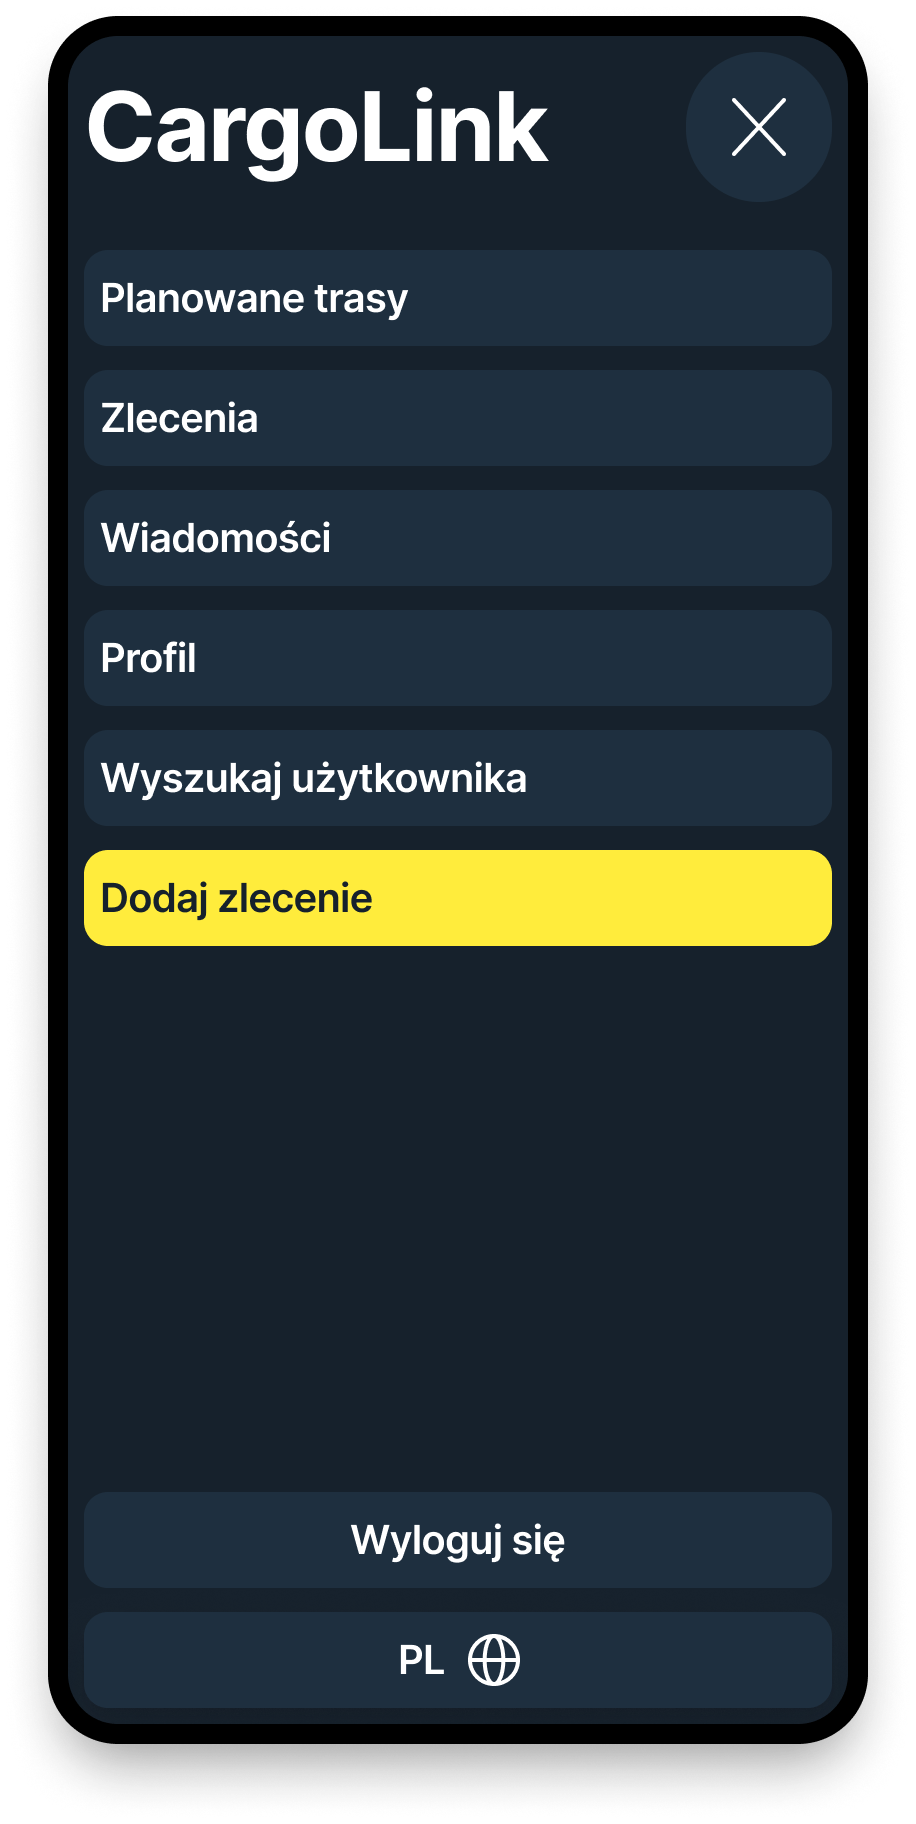
\includegraphics[width=0.3\linewidth]{rozdzial1/menu_m_zleceniodawca.png}}} &
    \vtop{\null\hbox{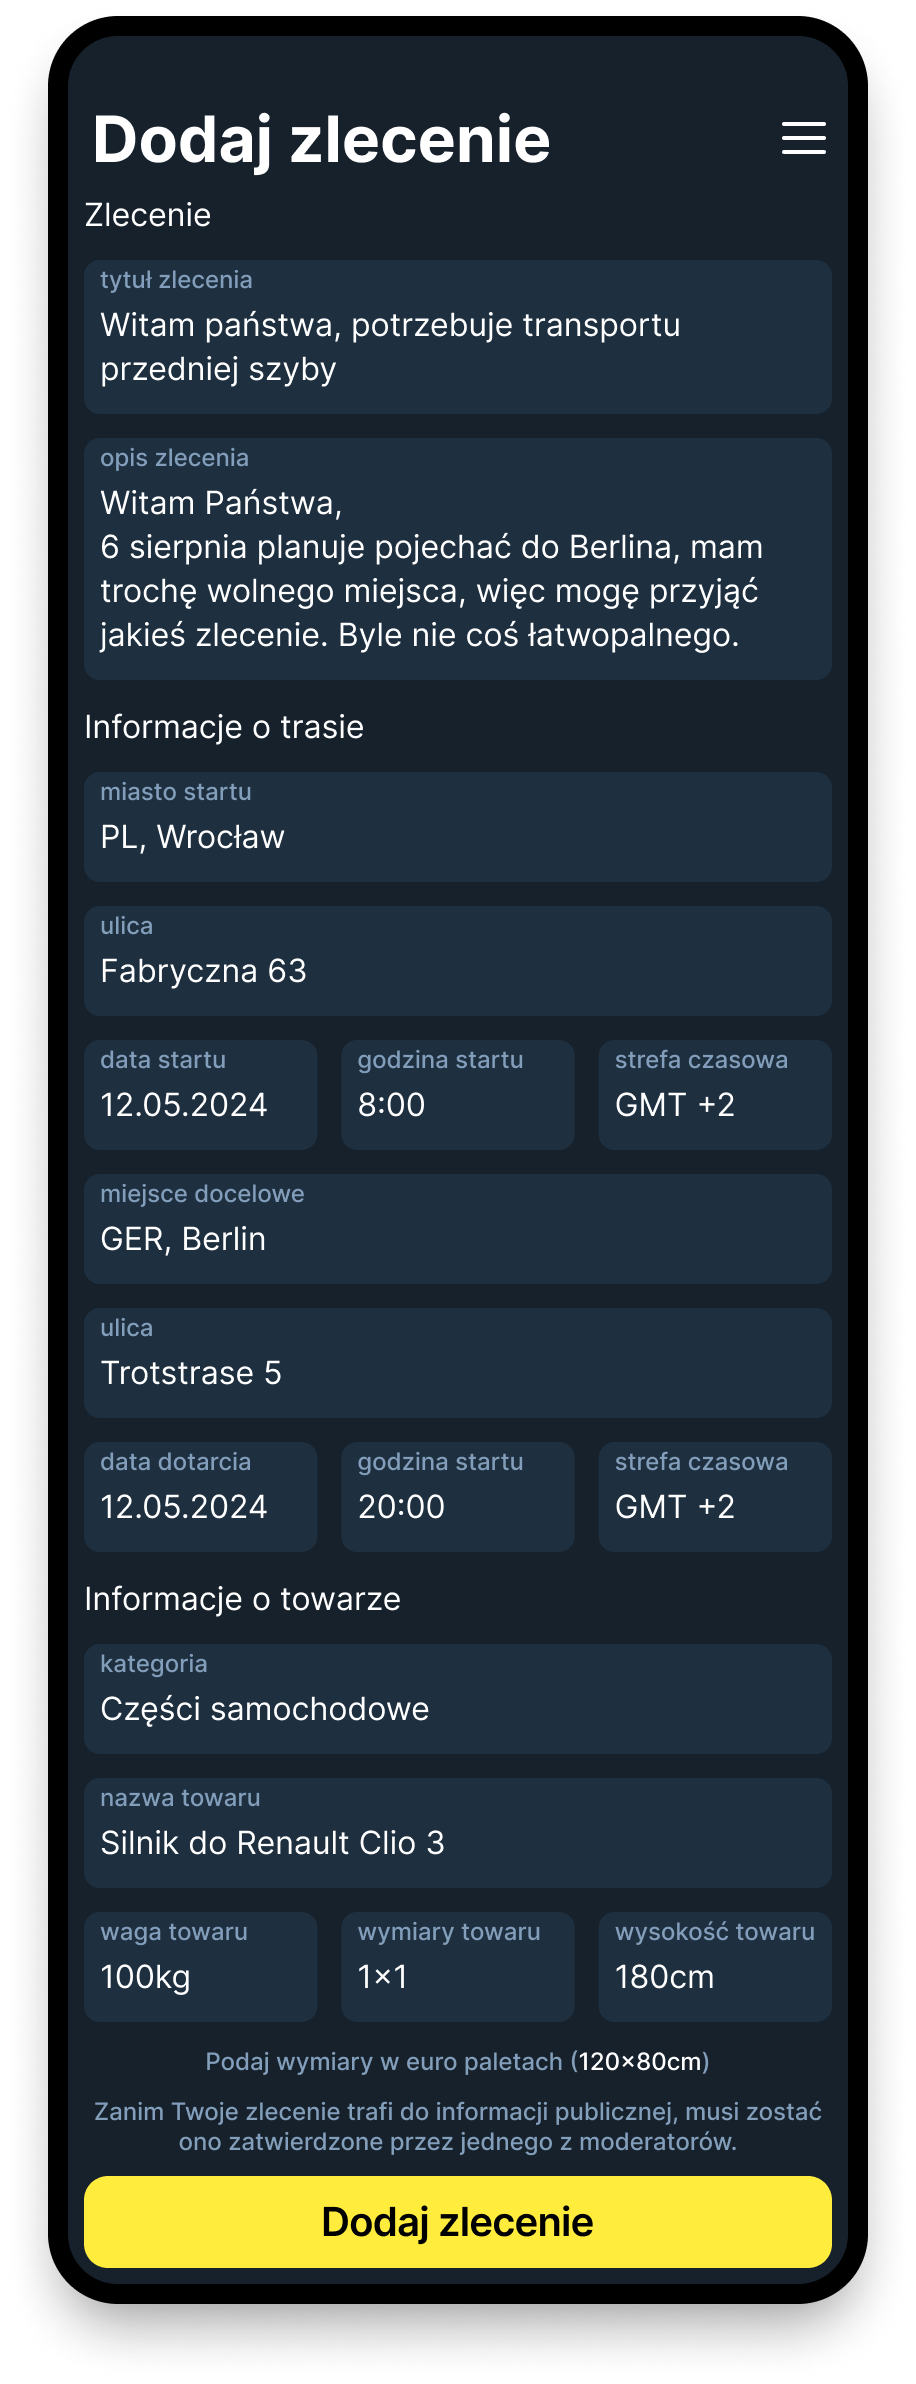
\includegraphics[width=0.3\linewidth]{rozdzial1/dodaj_zlecenie_m.png}}}
    \end{tabular}
    \caption{Dodawanie nowego zlecenia w wersji mobilnej: a) Menu po zalogowaniu jako zleceniodawca b) Formularz dodawania zlecenia}
	\label{Rys. fig:Dodawanie nowego zlecenia - ab - mobile}
\end{figure}
\begin{figure}[H]
 \centering
  \begin{tabular}{@{}ccc@{}}
  a) & b)\\
  \includegraphics[width=0.45\textwidth]{rozdzial1/menu_d_zleceniodawca.jpg} &
  \includegraphics[width=0.45\textwidth]{rozdzial1/dodaj_zlecenie_d.jpg}
  \end{tabular}
 \caption{Dodawanie nowego zlecenia w wersji desktopowej: a) Menu po zalogowaniu jako zleceniodawca b) Formularz dodawania zlecenia}
 \label{Rys. fig:Dodawanie nowego zlecenia - ab - desktop}
\end{figure}

\subsection{Moderator i Administrator}
\begin{figure}[H]
	\centering
		\includegraphics[width=\linewidth]{rozdzial1/PU_moderator_administrator.jpg}
	\caption{Diagram przedstawiający przypadki użycia aktorów \texttt{Moderator} i \texttt{Administrator}}
	\label{PU moderator administrator}
\end{figure}
Na powyższym diagramie przedstawione zostały przypadki użycia dla \texttt{Moderatora} oraz \texttt{Administratora}.  \\

 \texttt{Akceptacja nowych zleceń oraz ogłoszeń o planowanej trasie} \\
 Zdarzenie inicjujące: Kliknięcie w przycisk \texttt{Zgłoszenia do akceptacji (x)}. \\
 Warunki początkowe: Bycie zalogowanym jako moderator lub administrator. \\
 Przebieg podstawowy realizacji przypadku użycia: \\
 \begin{enumerate}
    \item Kliknięcie w przycisk \texttt{Zgłoszenia do akceptacji (x)} (Rys. \ref{Ackeptacja ogłoszenia - mobile - ab}.a lub \ref{Akceptacja ogłoszenia - destkop - ab}.a);
    \item Użytkownikowi wyświetla się lista oczekujących zgłoszeń;
    \item Osoba akceptująca zatwierdza lub odrzuca zgłoszenia klikając w odpowiednie przyciski (Rys. \ref{Ackeptacja ogłoszenia - mobile - ab}.b lub \ref{Akceptacja ogłoszenia - destkop - ab}.b).
 \end{enumerate}
 Warunki końcowe: Ogłoszenie zostaje odrzucone bądź zaakceptowane. \\
 \begin{figure}[H]
	\centering
	\begin{tabular}{@{}ccc@{}}
             a) & b)\\
     \vtop{\null\hbox{\includegraphics[width=0.3\linewidth]{rozdzial1/menu_moderator_m.png}}} &
     \vtop{\null\hbox{\includegraphics[width=0.3\linewidth]{rozdzial1/zatwierdz_m.png}}}
     \end{tabular}
     \caption{Akceptacja nowych zleceń i ogłoszeń o planowanej trasie w wersji mobilnej: a) Menu po zalogowaniu jako moderator lub administrator b) Panel akceptacji nowych ogłoszeń}
	\label{Ackeptacja ogłoszenia - mobile - ab}
 \end{figure}
 \begin{figure}[H]
  \centering
   \begin{tabular}{@{}ccc@{}}
   a) & b)\\
   \includegraphics[width=0.45\textwidth]{rozdzial1/menu_moderator_d.jpg} &
   \includegraphics[width=0.45\textwidth]{rozdzial1/zatwierdz_d.jpg}
   \end{tabular}
  \caption{Akceptacja nowych zleceń i ogłoszeń o planowanej trasie w wersji desktopowej: a) Menu po zalogowaniu jako moderator lub administrator b) Panel akceptacji nowych ogłoszeń}
  \label{Akceptacja ogłoszenia - destkop - ab}
 \end{figure}

 \texttt{Nadawanie i odbieranie użytkownikom prawa moderatora} \\
 Zdarzenie inicjujące: Wykonanie przypadku użycia \ref{Wyświetlenie profilu użytkownika}. \\
 Warunki początkowe: Bycie zalogowanym jako administrator. \\
 Przebieg podstawowy realizacji przypadku użycia: \\
 \begin{enumerate}
    \item Wykonanie przypadku użycia \ref{Wyświetlenie profilu użytkownika};
    \item Kliknięcie na pole \texttt{Typ użytkownika} rozwija listę z opcjami \texttt{Przewoźnik}, \texttt{Zleceniodawca}, \texttt{Moderator}, \texttt{Administrator} (Rys. \ref{Rys. fig:Profil użytkownika - mobile} lub \ref{Rys. fig:Profil użytkownika - desktop});
    \item Typ użytkownika zostaje zmieniony na wybraną opcje.
 \end{enumerate}
 Warunki końcowe: Typ użytkownika zostaje zmieniony na wybraną opcje. \\

\section{Projekt bazy danych}
Baza danych została wykonana w języku \texttt{PostgreSQL} \cite{PostgreSQL}. Jest to zaawansowany, open-source'owy system zarządzania bazami danych. Między innymi jest znany ze swojej elastyczności, skalowalności i zgodności ze standardami SQL.

Diagram bazy danych został wygenerowany przez program \texttt{DataGrip}. \texttt{DataGrip} to zaawansowane narzędzie do zarządzania bazami danych, stworzone przez JetBrains. Jest to wieloplatformowe środowisko IDE (zintegrowane środowisko programistyczne), które obsługuje wiele różnych systemów bazodanowych, takich jak \texttt{PostgreSQL}, \texttt{MySQL}, \texttt{Oracle}, \texttt{SQL Server}, \texttt{SQLite} i inne. Jedną z jego głównych zalet jest inteligentny edytor SQL, który oferuje funkcje automatycznego uzupełniania kodu, podpowiedzi dotyczących zapytań oraz wykrywania błędów w czasie rzeczywistym. \texttt{DataGrip} umożliwia również łatwe przeglądanie struktury baz danych, poprzez graficzny interfejs. Narzędzie jest szczególnie cenione przez deweloperów i administratorów baz danych za swoją intuicyjność.

\begin{figure}[H]
	\centering
		\includegraphics[width=1\linewidth]{rozdzial1/baza_danych.jpg}
	\caption{Projekt bazy danych}
	\label{Rys. fig:Projekt bazy danych}
\end{figure}

Dla tabel zastosowano nazewnictwo w języku angielskim, co jest dobrą praktyką podczas pracy w zespołach międzynarodowych, ułatwiając współpracę i zrozumienie struktury danych. Klucze główne we wszystkich tabelach są typu \texttt{UUID}, co jest nowoczesnym podejściem do identyfikacji wierszy w bazach danych. W odróżnieniu od tradycyjnych kluczy głównych opartych na auto inkrementujących liczbach całkowitych, \texttt{UUID} są unikalnymi identyfikatorami, które mogą być generowane niezależnie w różnych systemach bez ryzyka konfliktów. Jest to szczególnie istotne w systemach rozproszonych, gdzie wiele serwerów może dodawać dane równocześnie. Co więcej, \texttt{UUID} zwiększa bezpieczeństwo, ponieważ trudno jest przewidzieć kolejny identyfikator, co może mieć znaczenie w aplikacjach wymagających większej prywatności i bezpieczeństwa danych. \\
Przykładowy klucz główny UUID: \texttt{2d8e72dc-aa4e-4c4c-b02b-b08655d891aa} \\

Dodatkowo, zamiast przechowywać hasła w postaci zwykłego tekstu, hasła użytkowników są szyfrowane przy użyciu algorytmu \texttt{bcrypt}. Dzięki któremu nawet w przypadku nieautoryzowanego dostępu do bazy danych, hasła pozostają bezpieczne, ponieważ odzyskanie oryginalnej wartości z hasha jest praktycznie niemożliwe. Dodatkowo technika solenia (and. \texttt{salt}) stosowana w \texttt{pgcrypto} (rozszerzenie do \texttt{PostgreSQL}) dodaje losowy ciąg znaków do każdego hasła przed jego zahashowaniem, co zapobiega atakom typu "rainbow table" i sprawia, że dwa identyczne hasła będą miały różne zaszyfrowane wartości. \\
Przykładowe zaszyfrowane hasło: \\
\texttt{\$2a\$06\$M/okyRSZvHY80DUo6rlTi.SNaZCZF5/NisSB5PMZCPeaPwnFZplAy}. \\
Po odszyfrowaniu okazuje się, że ukryty ciąg znaków to: \texttt{twojehaslo} \\

Do przechowywania informacji o współrzędnych geograficznych w tabeli \texttt{Addresses}, użyto typu danych \texttt{geography(point,4326)}. Ten typ danych pozwala na precyzyjne przechowywanie współrzędnych geograficznych zgodnych z globalnym systemem odniesienia WGS 84. Umożliwia to wykonywanie zaawansowanych operacji geograficznych, takich jak obliczanie odległości czy znajdowanie punktów w określonym promieniu. \\
Przykładowa wartość tego typu danych może wyglądać w następujący sposób: \\
\texttt{0101000020E61000004B598638D68D4940E0F3C308E1093140} \\
Odpowiednią kwerendą, uzyskać możemy szerokość i wysokość geograficzną \\
{\belowcaptionskip=-9pt
\begin{lstlisting}[language=SQL,caption=Przykład kwerendy SQL, label=lst:sql_query]
SELECT ST_X(addresses.geography::geometry) AS longitude, 
       ST_Y(addresses.geography::geometry) AS latitude 
FROM addresses;
\end{lstlisting}
}
W tym przypadku jest to szerokość: 51.1081 oraz wysokość 17.03859, czyli współrzędne geograficzne Wrocławia.